\documentclass{report}

\usepackage[utf8]{inputenc} 
\DeclareUnicodeCharacter{F076}{-} % this bullet point is in some documents...
\usepackage[T1]{fontenc}
\usepackage[french]{babel}
\usepackage{xspace} % For space after \fg...

\usepackage{lmodern} % Fonts

\usepackage{setspace} % for line spacing
\spacing{1.5}
\usepackage[top=2.5cm, bottom=2.5cm, left=2.5cm, right=2.5cm]{geometry} % for margins

\usepackage{calc} % cannot remember... ? Maths ?
\usepackage{amsmath} % for math
\usepackage{amssymb} % for math
\usepackage{mathrsfs} % for math

\usepackage{graphicx} % to include images

\usepackage{array,multirow,makecell,tabularx, longtable} % to manage table outputs
\renewcommand\tabularxcolumn[1]{>{\centering\arraybackslash}m{#1}} % center by default tabularx
\newcolumntype{P}[1]{>{\centering\arraybackslash}p{#1}} % new centered p-type column
\usepackage{booktabs} % cant remember...
\usepackage{floatrow} % to have floats side by side (ex : figure with associated table)
% Table float box with bottom caption, box width adjusted to content
\newfloatcommand{capbtabbox}{table}[][\FBwidth] % cant remember, got it of the web
\usepackage{caption} % enables to caption non floating table or figures

\usepackage{rotating}
\usepackage{lscape}
\usepackage{multicol}
\setlength{\columnsep}{0.5cm}

\usepackage{pdfpages}

\usepackage{listings}
\lstset{
breaklines=true,
extendedchars=true,
literate={é}{{\'e}}1,
}
\usepackage{minted}

\usepackage{url}
\usepackage{hyperref}

\usepackage{titlesec} 
\titleclass{\part}{top} % changing part so that it does not take a full page.
\titleformat{\part}
    [display] % shape
    {\centering\normalfont\Huge\bfseries} % format
    {\MakeUppercase{\partname}\vspace{1pc}} % label
    {0pt} % set between label and title body
    {\titlerule[2pt]\vspace{1pc}\Huge\MakeUppercase} % before body
\titlespacing*{\part}
    {0pt} % left 
    {0pt} % before sep
    {10pt} % after sep

\titleclass{\chapter}{straight} % make chapter like a section (no newpage)
\titleformat{\chapter}
    [display] % shape
    {\centering\normalfont\huge\bfseries} % format
    {\chaptertitlename ~\thechapter} % label 
    {0pt} % sep between label and title body
    {\huge\MakeUppercase} % before body
\titlespacing*{\chapter}
    {0pt} % left
    {20pt} % before sep
    {20pt} % after sep

\usepackage{chngcntr}
\counterwithout{figure}{chapter}
\counterwithout{table}{chapter}
    

\newcommand{\emphbox}[1]{
    \vspace{5mm}
    \noindent\fbox{ 
        \begin{minipage}[c]{\linewidth}
            {\em #1}
        \end{minipage}
    }
}

\newcommand{\reffig}[1]{F\textsc{igure}~\ref{#1} page~\pageref{#1}}

\newcommand{\reftable}[1]{T\textsc{able}~\ref{#1} page~\pageref{#1}}

\newcommand{\mref}[1]{\ref{#1} page~\pageref{#1}}

\title{Extraction des ingrédients depuis les fiches techniques de produits alimentaires}
\author{Pierre \textsc{massé}}
\date{Juin 2020}

\begin{document}

\maketitle

\large
\begin{abstract}   
    
    La gestion de l'information produit est devenu un enjeu de société majeur ces dernières années.
    Les scandales sanitaires récents ont déclenché une prise de conscience collective des consommateurs, en parallèle de la mise en place de réglementations de plus en plus contraignantes pour l'ensemble des acteurs de la filière~\cite{incotext}\cite{incoexpl}.
%    \`{A} ce titre, le Groupe Pomona a lancé ces dernières années un projet majeur de refonte des processus et des outils de gestion de l'information produit.

%    La première filiale du groupe a fait l'objet d'un déploiement réussi, mais cela a toutefois mis en évidence le fait que des gains à la fois en qualité et en productivité restent accessibles.

    La mise en place d'outils mettant en oeuvre les principes du Machine Learning appliqués au traitement du langage permettrait d'aider les opérationnels de la gestion de l'information à interpréter plus vite et mieux les documents mis à disposition par les fournisseurs du groupe.
    Le présent rapport détaille la mise en place d'un outil permettant d'extraire les listes d'ingrédients des fiches techniques transmises par les fabricants des produits.

    Dans une première partie, on détaillera le contexte métier autour de la gestion de l'information produit. 
    Nous nous analyserons ensuite les données disponibles, et les possibilités de les exploiter.
    Nous expliciterons alors les raisons qui ont poussé à choisir le cas d'usage, et la manière dont il pourrait être mis en oeuvre au sein du Groupe Pomona.
    La quatrième partie sera consacrée à la construction du modèle à proprement parler, et la dernière partie ouvrira la réflexion sur les travaux à venir.


\end{abstract}
\normalsize

\tableofcontents

\part{Contexte métier}

    \chapter{Description du Groupe}

    \large
    L'objet de l'ensemble de cette première partie est de donner sur le Groupe Pomona des éclairages nécessaires à la compréhension du cas d'usage développé.
    Bien d'autres aspects sur la société, pourraient être mentionnés (ex : des indicateurs sur l'activité, l'histoire du Groupe\dots) mais ils seront omis car non indispensables à la compréhension du sujet.
    Plus de détails sur le Groupe sont accessibles sur le site web de la société\cite{site_pomona}.
    \normalsize    

        \section{Le métier du Groupe Pomona}
        \label{business}

        Le Groupe Pomona est une société de distribution livrée de produits alimentaires à destination des professionnels des métiers de bouche.
        L'activité du Groupe consiste uniquement à acheter et revendre de la marchandise, à l'exclusion de toute activité de fabrication ou de transformation\footnote{de très rares cas de transformation existent (ex : mûrissage de fruits, filetage de poisson) mais sont extrêmement exceptionnels}. Le Groupe Pomona est une société de \emph{distribution}. Elle ne possède d'ailleurs pas d'actif industriels (autre que des entrepôts logistiques) ni d'agréement pour transformer les marchandises.        
        
        Cette activité d'achat/vente se fait dans la majorité des cas sous le régime du \emph{négoce}, à savoir que le Groupe acquiert la propriété des marchandises qu'il commercialise avant de la céder à ses clients.
        L'autre régime est celui dit de la \emph{prestation (logistique)}.
        Dans ce cas, par le jeux d'écritures comptables, la valorisation du stock disparaît des comptes du Groupe.
        Néanmoins, indépendamment de cet aspect purement comptable, l'ensemble :
        \begin{description}
            \item[des flux de documents :] commandes d'achat, factures fournisseur, commandes de vente, factures clients
            \item[des flux financiers :] paiements fournisseur, paiements client
            \item[des flux physiques :] réception et stockage, préparation et expédition
        \end{description}
        restent largement inchangés.
        
        Pour résumer, l'activité de l'ensemble des entités du Groupe pourraient se résumer via le schéma présenté à la \reffig{fig:flux metier}

        \begin{figure}[htbp]
            \begin{center}
            \includegraphics[width=\linewidth]{img/Les flux métier de Pomona.png}
            \end{center}
            \caption{Les flux métier avec les partenaires commerciaux}
            \label{fig:flux metier}
        \end{figure}

        \emphbox{Le métier du Groupe est d'être un \emph{grossiste}, qui achète et revend des produits alimentaires\footnotemark \ \emph{sans produire ou transformer quoi que ce soit}.}
        \footnotetext{dans la grande majorité des cas, cf. \emph{Les produits non-alimentaires} \mref{produits_nonal}}

        \section{La décentralisation}
        
        Le Groupe Pomona est un Groupe fortement décentralisé, avec des organisations largement indépendantes les unes des autres. 

            \subsection{Les Directions fonctionnelles}

            Pour des raisons évidentes de recherche de synergies ou de conformité réglementaires, certaines activités restent toutefois mutualisées à la maille du Groupe.
            Il s'agit des organisations suivantes :
            \begin{description}
                \item[La Direction Administrative et Financière (DAF) :] regroupe les équipes comptables Groupe, l'audit interne et la consolidation financière
                \item[La Direction Qualité :] est en charge de définir et contrôler l'application des standard de qualité
                \item[La Direction des Systèmes d'Information (DSI) :] développe et maintient en condition opérationnelles les systèmes d'information du Groupe
                \item[La Direction Technique et Logistique (DTL) :] est en charge des projets immobiliers (entrepôts), des négociations avec les transporteurs et joue un rôle de conseil interne sur les sujets logistiques
                \item[La Direction des Ressources Humaines :] se charge de l'ensemble des aspects en lien avec le recrutement, la paye et les sujets sociaux
                \item[La Direction Commerciale Groupe (DCG) :] définit une stratégie et des bonnes pratiques commerciales et marketing
            \end{description}

            \subsection{Les clients du Groupe}
            \label{clients}

            Afin de comprendre l'organisation du Groupe, il est nécessaire de connaître la typologie de ses clients.
            Comme mentionné précédemment, le Groupe s'adresse exclusivement aux professionnels des métiers de bouche.
            Aucune marchandise n'est vendue à des particuliers.
            Les principales typologies de clients sont les suivantes : 
            \begin{description}
                \item[Les Sociétés de Restauration :] elles exploitent les restaurants d'entreprise et certaines cantines d'établissement d'enseignement supérieur
                \item[Les Marchés Publics :] regroupent les clients qui dépendent des collectivités (écoles, hôpitaux, prisons, \dots)
                \item[La restauration commerciale :] est l'ensemble des restaurants à vocation commerciale, qu'ils soient chaînés (hippopotamus, O'Tacos, \dots) ou indépendants (\og le restaurant du coin \fg)
                \item[Les spécialistes :] il s'agit des détaillants spécialisés qui s'adressent aux particuliers. Boulangers, pâtissiers, bouchers, traiteurs, vente à emporter, \dots
                \item[Les Grandes et Moyennes surfaces (la GMS) :] sont les enseignes de la grande distribution. En général, l'accès à ces clients est compliqué par les règles mises en place par leurs centrales d'achat. Il représentent en général qu'un canal de vente d'opportunité.
            \end{description}

            Les trois premières de ces catégories représentent ce que l'on appelle la \emph{Restauration Hors Domicile (RHD)} (ou parfois également la Restauration Hors Foyer, RHF).

            \subsection{Premier niveau de décentralisation : les branches}
            \label{les_branches}
            Le Groupe Pomona est divisé en branches, qui sont des organisations indépendantes et qui ont toute latitude pour gérer leurs stratégie et politique commerciales, la gestion de leurs achats, leur stratégie marketing, \dots
            En particulier, les systèmes d'information ne sont pas identiques entre les différentes branches.
            Afin d'éviter de se concurrencer entre elles, leurs domaines d'activité respectifs ont été partitionnés par familles de produit commercialisés, segments client cibles et géographie. 

                \subsubsection{Les branches RHD}
                
                Les branches RHD s'adressent comme leur nom l'indique aux client de la Restauration Hors Domicile (cf. section \mref{clients}) en France.
                Elles se répartissent ce marché en travaillant des gammes de produits distinctes.
                Il s'agit des branches historiques du Groupe, qui représentent l'essentiel de son chiffre d'affaire.
                La répartition par produit est la suivante :
                \begin{description}
                    \item[PassionFroid :] spécialiste des \emph{produits surgelés, de la viande fraîche et des produits laitiers}
                    \item[\'{E}piSaveurs :] spécialiste des produits qui se conservent à température ambiante : \emph{produits d'épicerie, conserves, boissons et consommables de cuisine non-alimentaires}
                    \item[TerreAzur :] spécialites des \emph{Fruits et Légumes frais, et Produits De la Mer frais} 
                \end{description}
                La non-concurrence entre les branches est assurée par le fait qu'elles ne commercialisent pas les mêmes produits.
                Bien que nommées RHD, elles peuvent également vendre leurs produits à la grande distribution, mais généralement ces marchés sont verrouillés par les centrales d'achat des grandes enseignes.
                De plus, les branches RHD utilisent le progiciel SAP comme système de gestion.
                La branche TerreAzur est en cours de déploiement, en 2020 environ les 2 tiers des succursales travaillent avec ce progiciel.

                \subsubsection{Les branches spécialistes}

                Les branches spécialistes s'adressent aux clients dits spécialistes (cf. section \mref{clients}) en France.
                Elles sont en mesure de commercialiser tout type de produit pour répondre aux besoins de leurs clients.
                En particulier, elles peuvent tout à fait commercialiser certains produits qui sont également vendus par les branches RHD.
                Elles se répartissent la clientèle spécialiste de la manière suivante :
                \begin{description}
                    \item[Délice et Création :] s'addresse aux \emph{Boulangers et Pâtissiers}
                    \item[Saveurs d'Antoine :] s'adresse aux \emph{Bouchers, Charcutiers et Traiteurs}
                    \item[Relais d'Or :] s'addresse à la \emph{restauration indépendante nomade}
                \end{description}
                Comme pour les branches RHD, ces branches peuvent lorsqu'elles en ont l'opportunité vendre leurs produits à la GMS.

                \subsubsection{L'étranger}

                Bien que le Groupe Pomona soit une société dont l'essentiel de l'activité est faite sur le marché français, deux réseaux sont en cours de constitution sur des pays limitrophe.
                Ces branches sont susceptibles de travailler tout type de produit, à destination de tout type de client.
                Elles sont positionnées sur les marchés suivants : 
                \begin{description}
                    \item[Pomona Suisse :] présente sur le marché Suisse
                    \item[Pomona Iberia :] présente sur le marché Espagnol 
                \end{description}

                On peut synthétiser la répartition de l'activité par branche de la manière présentée à la \reffig{fig:repartition_activite}.

                \subsubsection{Les produits non-alimentaires}
                \label{produits_nonal}
                Si l'essentiel des produits commercialisés par les branches du Groupe sont des produits alimentaires, comme évoqué précédemment une partie de l'activité commerciale se fait tout de même autour de produits non-alimentaires.
                Ces produits restent malgré tout destinés exclusivement aux professionnels des métier de bouche, et il s'agit de consommables (par opposition à des articles d'électroménager, de la vaisselle non-jetable, \dots).

                On distingue en général deux catégories de produits non-alimentaires : 
                \begin{itemize}
                    \item les produits dits \og d'hygiène \fg
                    \item les produits dits \og de chimie \fg
                \end{itemize}

                Les produits de chimie regroupent les produits qui doivent faire l'objet d'une fiche de données de sécurté au sens du réglement Européen No 1907/2006 dit \og REACH \fg (Registration, Evaluation, Authorisation and Restriction of Chemicals) \cite{reach_text}.

                Les produits d'hygiène regroupent tous les autres produits non-alimentaires.
                L'appelation \og d'hygiène \fg est donc réductricte, dans la mesure où cette large famille regroupe les consommables de nettoyage (éponges, papiers absorbants, \dots) mais également tout type d'autres consommables (serviettes de tables, gobelets en plastiques, pics à brochettes, boîtes de produits à emporter, \dots).

                \emphbox{La commercialisation de produits non-alimentaires existe au sein du Groupe, mais on se focalisera pour la suite sur les produits alimentaires qui reste le coeur de métier.}

                \begin{figure}[htpb]
                    \begin{center}
                    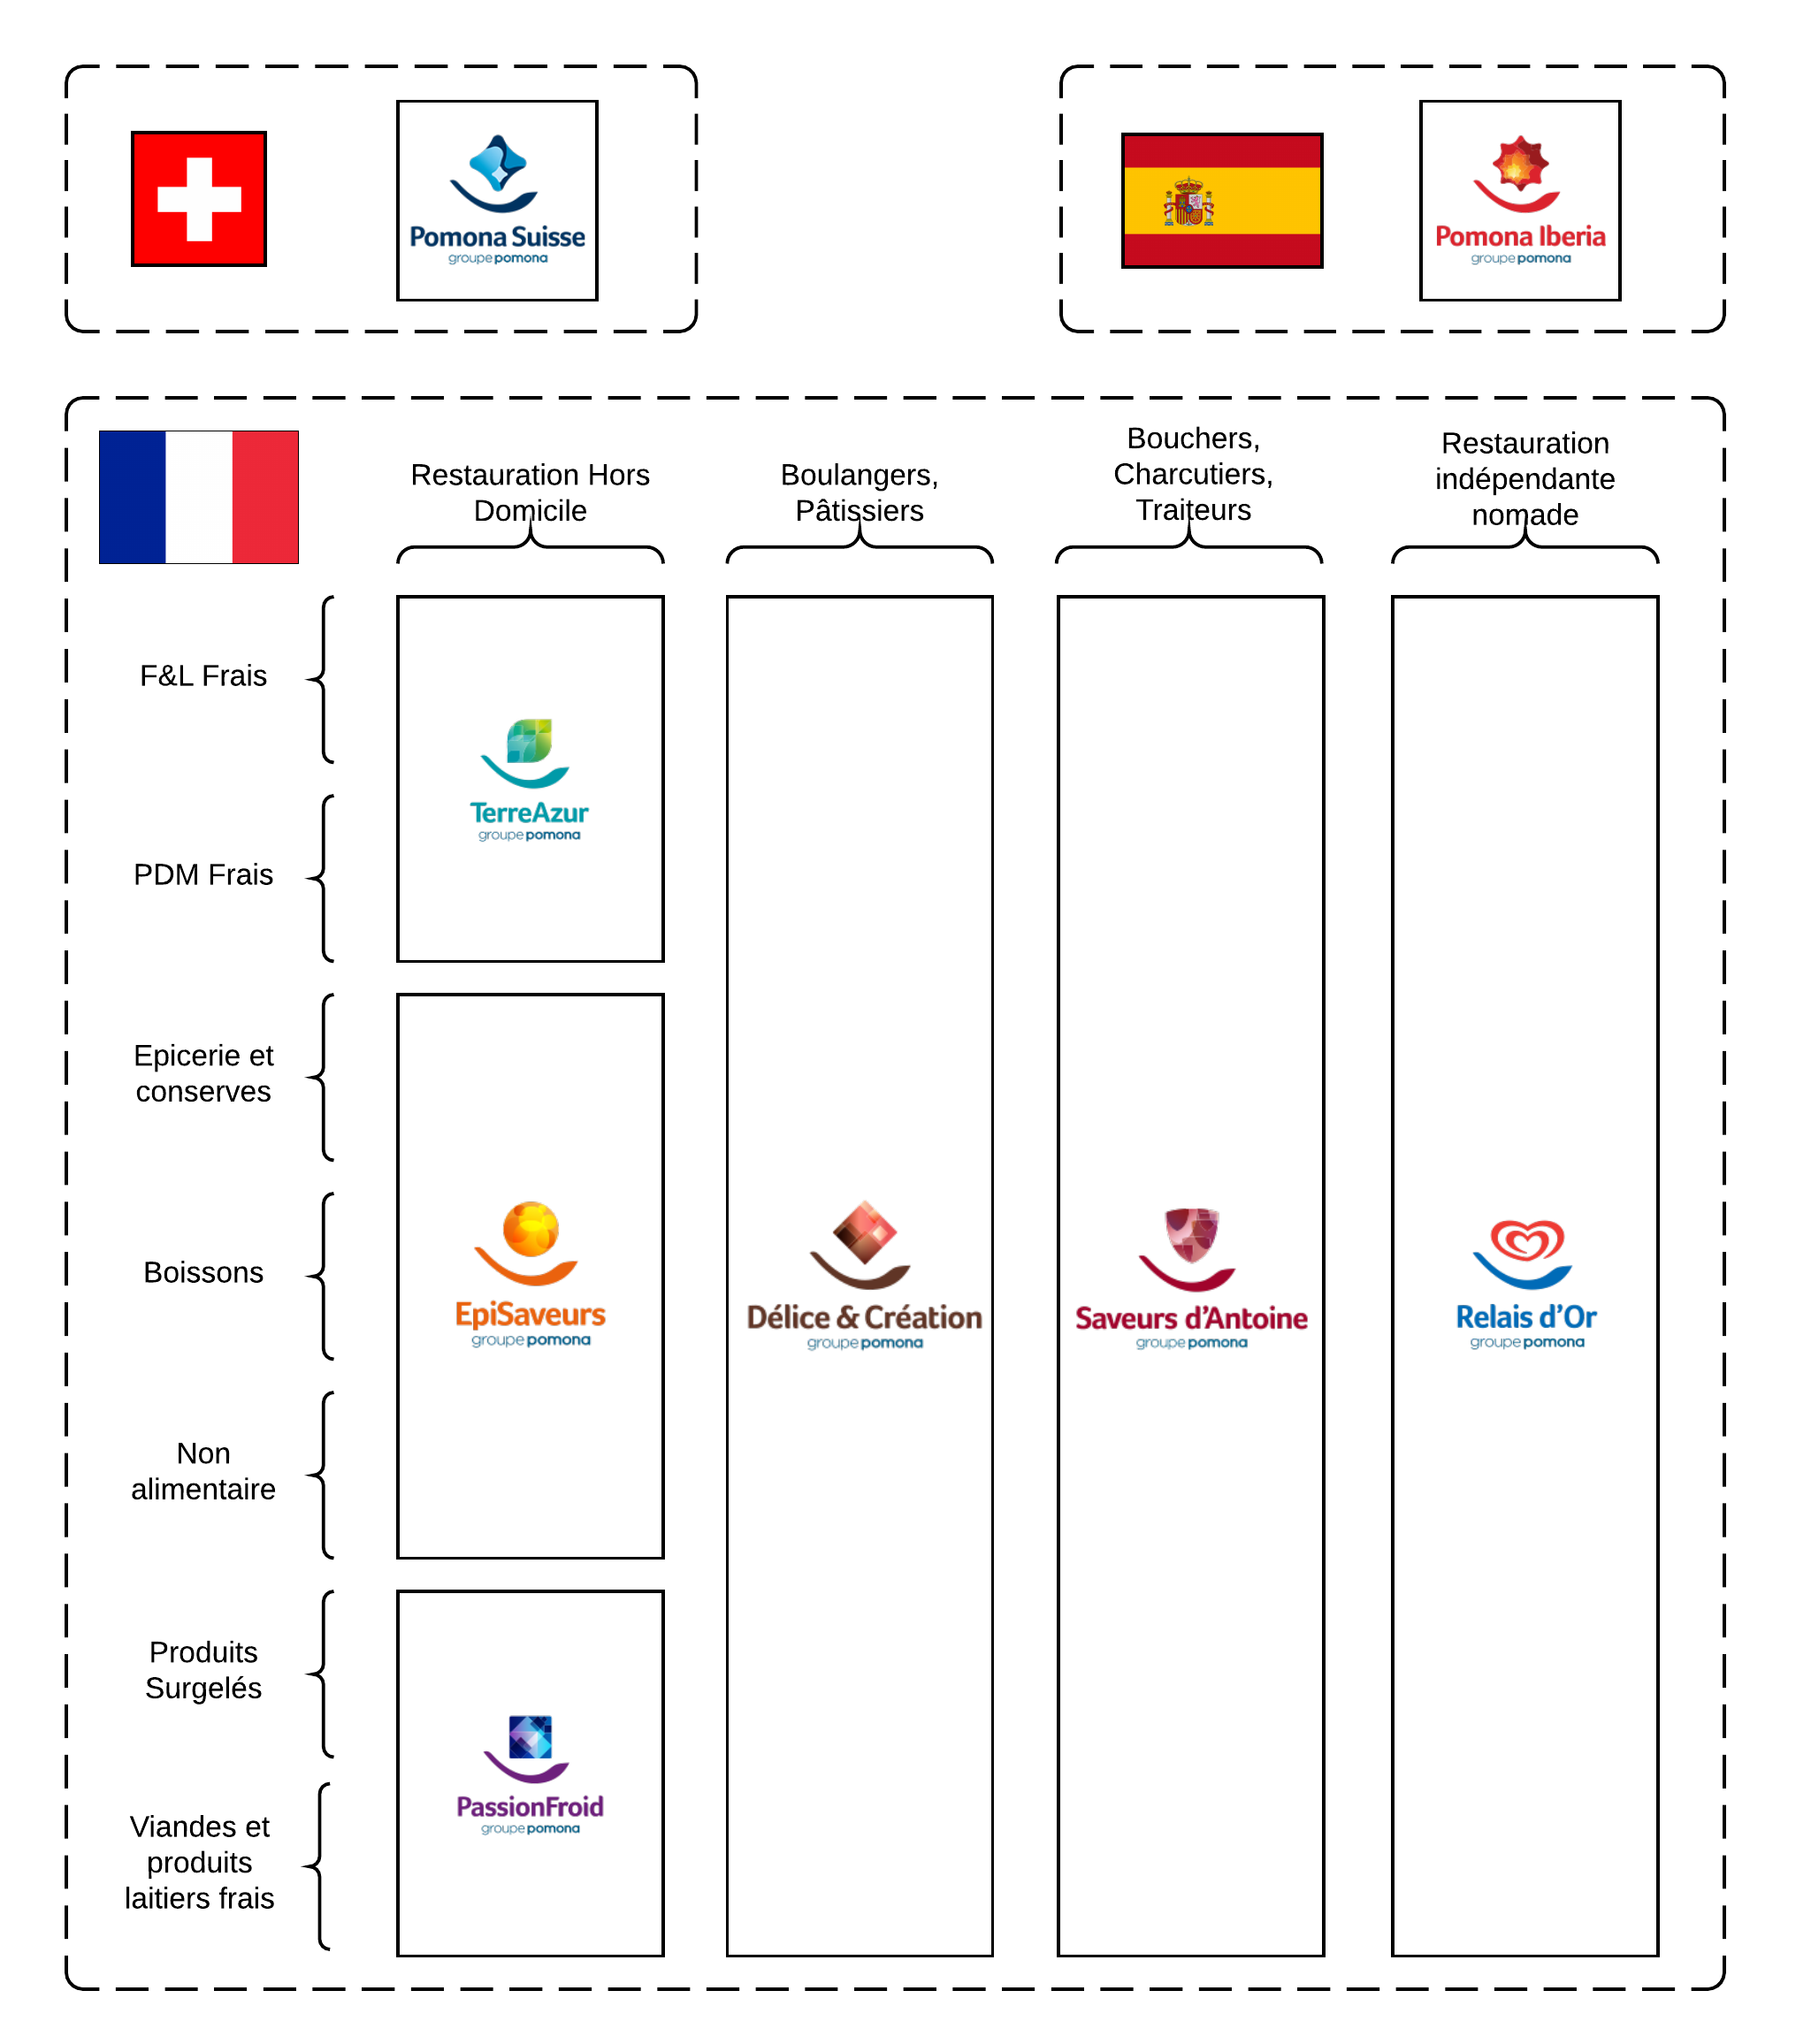
\includegraphics[width=\linewidth]{img/La répartition de l'activité des branches.png}
                    \end{center}
                    \caption{La répartition de l'activité des branches}
                    \label{fig:repartition_activite}
                \end{figure}

            \subsection{Le second niveau de décentralisation : les succursales}

            Chacune des branches est elle-même à son tour décentralisée en un réseau d'entrepôts régionaux : les succursales (parfois également appelées simplement \og régions\fg).
            Ces succursales sont gérées comme des PME indépendantes, avec un directeur et un compte de résultat qui leur est propre.
            Si certaines négociation avec des fournisseurs ou des clients nationaux sont parfois menée par les branches, les succursales sont autonomes dans :
            \begin{itemize}
                \item{la définition de leur assortiment, même si des contraintes s'appliquent}
                \item{la stratégie de développement commercial}
                \item{la négociation des prix d'achat}
                \item{la négociation des prix de vente}
                \item{la politique de rémunération de leurs employés}
            \end{itemize}
            
            \`{A} ce titre, elles ont leurs propres équipes d'achat, leurs équipes commerciales (télévente et vente route), leurs équipes administratives et évidemment leurs équipes logistiques (essentiellement en entrepôt et les chauffeurs livreurs en charge des livraisons client).

            Certaines activités restent de la responsabilité des équipes centrales des branches, comme : la négociation avec les clients ou les fournisseurs nationaux, la constitution de l'assortiment commun (les produits que toutes les succursales doivent détenir), la gestion des référentiels de données de base métier, \dots
            
            Un exemple de maillage régional est présenté en \reffig{fig:reseau_es}, sachant que ce maillage régional est différent pour chacune des branches.
            \begin{figure}[htpb]
                \begin{center}
                \includegraphics[width=\linewidth]{img/réseau es.png}
                \end{center}
                \caption{Le maillage régional de la branche \'{E}piSaveurs}
                \label{fig:reseau_es}
            \end{figure}


    \chapter{La gestion de l'information produit}
    
    \large
    Ce chapitre a pour vocation à éclairer les aspects métier en lien avec la gestion de l'information produit. 
    C'est le seul processus métier qui sera détaillé dans la mesure où c'est uniquement celui qu'il est nécessaire de connaître pour comprendre les cas d'usage développés ultérieurement.
    \normalsize

        \section{L'information produit}
        
            \subsection{Utilisations de l'information produit}
            \label{utilisation_info_produit}

                \subsubsection{Conformité réglementaire}
                La gestion de l'information produit est essentiellement une contrainte réglementaire à statisfaire.
                Comme mentionné au préambule, la réglementation autour de l'information des consommateur s'est sans cesse complétée au cours des dernières années.
                Un des textes centraux est le règlement n°1169/2011 dit INCO (INformation COnsommateur)\cite{incotext}\cite{incoexpl}.
                C'est ce règlement qui définit l'ensemble des informations qui doivent être étiquetées sur le produit (liste d'ingrédients, tableau de données nutritionnelles, \dots), mais également affichée au client lors de commande en ligne sur les sites de e-commerce.
                Il s'agit principalement d'informations relatives à la sécurité alimentaire (ex : les allergènes) ou la santé (ex : informations nutritionnelles).

                \subsubsection{Attentes client}

                Les consommateurs finaux (les \og convives \fg) étant de plus en plus sensibles au contenu de leur assiète, les clients du Groupe sont de plus en plus demandeurs d'information relatives aux produits qu'ils commandent.
                Ils demandent donc régulièrement des informations qui vont au-delà de ce qui est normalement prévu par la réglementaition.

                De plus, sur certains marchés pour lesquels des contrats courant sur de longues périodes - jusqu'à un an - sont établis (les marchés publics sont très concernés), il n'y a pas d'échantillonnage des produits.
                La seule manière pour ces clients d'évaluer la qualité des produits est de se référer aux documents contenant les informations produit, fournis par les distributeurs.

                \subsubsection{Gestion}

                Certaines informations relatives au produits sont nécessaires pour des raison de gestion adminsitrative.
                Par exemple, la gestion des taxes sur les produits alimentaires est complexe : 
                \begin{itemize}
                    \item les taux de TVA sont variables en fonction du type de produit
                    \item des taxes spécifiques s'appliquaient aux produits contenant de l'huile ou de la farine
                    \item des règlements particuliers s'appliquent aux alcools
                    \item \dots
                \end{itemize}
                D'autres informations, comme la nomenclature douanière, sont nécessaires pour effectuer les déclarations auprès des douanes européennes.

                Un autre type d'information capital pour la gestion des flux d'achat et de vente sont les informations logistiques, qui définissent par exemple le nombre d'unités consommateur dans le colis, le nombre de colis sur une palette, \dots
                Une gestion rigoureuse de ces information est indispensable pour que les flux d'achat ou de vente soient correctement exécutés (que les quantités commandées soient les bonnes, que les montants facturés soient corrects, \dots).

            \subsection{Des produits bruts aux produits transformés}

            Le niveau d'exigence en termes d'information produit est variable en fonction du niveau de transformation de ce produit.
            Par exemple, sur des fruits et légumes frais, à peu de choses près seul le pays d'origine doit être affiché au client.
            Sur une barre chocolatée, ou un plat cuisiné, il sera nécessaire d'afficher :
            \begin{itemize}
                 \item une liste d'ingrédients (mettant en évidence les allergènes)
                 \item un tableau de données nutritionnelles (protéines, gludcides, \dots)
                 \item une dénomination réglementaire
            \end{itemize}

            \subsection{Les grands types d'information}
            \label{info_produit}

            On se focalisera dans ce paragraphe sur les informations relatives aux \emph{produits alimentaires}.

                \subsubsection{La composition}
                \label{composition}

                La première grande famille de données réglementaires sont les données de composition.
                Elles détaillent quels sont les ingrédients qui sont mis en oeuvre dans la fabrication des produits.
                \'{E}videmment, la composition a en général plus de sens que pour les produits transformés que pour les produits bruts.
                Elle peut prendre la forme d'un texte listant la liste des ingrédients (l'étiquetage de ce texte est en général obligatoire sur les emballages des produits), ou d'un tableau.
                
                Les ingrédients incluent également les additifs.
                Il s'agit de substances ajoutées à la recette pour répondre à des fonctions particulières (colorant, exhausteur de goût, émulsifiant).
                Elles ne représentent en général un pourcentage en masse négligeable dans la composition totale du produit.

                Le pourcentage en masse est parfois inclus sur certains ingrédients. 
                La règlementation l'oblige dans certains cas, par exemple quand l'ingrédient en question est mentionné dans la dénomination du produit (pour une \emph{tarte aux framboises}, la proportion de framboise doit être mentionnée dans la composition).

                Enfin, un aspect à la fois règlementaire et particulièrement important est la présence d'allergènes dans la composition.
                Le règlement INCO\cite{incotext}\cite{incoexpl} impose de mettre en évidence les allergènes relevant d'une des 14 catégories suivantes :
                \begin{enumerate}
                    \item Céréales contenant du gluten, à savoir blé, seigle, orge, avoine, épeautre, kamut ou leurs souches hybridées, et produits à base de ces céréales
                    \item Crustacés et produits à base de crustacés
                    \item \OE ufs et produits à base d’ \oe ufs
                    \item Poissons et produits à base de poissons
                    \item Soja et produits à base de soja
                    \item Lait et produits à base de lait (y compris le lactose)
                    \item Fruits à coque, à savoir: amandes, noisettes, noix, noix de cajou, noix de pécan, noix du Brésil, pistaches, noix de Macadamia ou du Queensland, et produits à base de ces fruits
                    \item Céleri et produits à base de céleri
                    \item Moutarde et produits à base de moutarde
                    \item Graines de sésame et produits à base de graines de sésame
                    \item Anhydride sulfureux et sulfites
                    \item Lupin et produits à base de lupin
                    \item Mollusques et produits à base de mollusques
                \end{enumerate}
                Il peut y avoir deux niveaux de présence d'un allergène dans un produit (au-delà de la simple absence) :
                \begin{description}
                    \item[intentionnellement mis en oeuvre :] dans le cas où un ingrédient allergène fait volontairement partie de la recette. Ex : présence de moutarde dans un plat cuisiné.
                    \item[contamination croisée :] par exemple lorsque le produit fini est issu d'une chaîne de transformation qui traite un ingrédient allergène, mais que cet ingrédient ne fait pas partie de la recette. Ce cas de figure est en général mis en évidence par des mentions telles que \emph{"Peut contenir des traces de soja"} ou bien \emph{"Transformé dans un atelier processant également des fruits à coques et du sésame"}.
                \end{description}

                \subsubsection{Les informations nutritionnelles}

                Une autre grande famille d'information produit sont les informations nutritionnelles. 
                Elles détaillent la quantité des principaux nutriments contenus dans les produits.
                Certains d'entre eux sont rendus obligatoires par le règlement INCO~\cite{incotext}\cite{incoexpl} cf. l'exemple de tableau à la \reftable{tab:donnees_nut}, et d'autres sont optionnels, comme par exemple la quantité de fer, de calcium, \dots

                \begin{table}[htbp]
                    \begin{center}
                    \begin{tabularx}{\linewidth}{|X|X|X|X|}
                        \hline
                        \textbf{Informations nutritionnelles} & \textbf{Pour 100g} & \textbf{Pour un biscuit} & \textbf{\% des AJR pour un biscuit} \\
                        \hline
                        \'{E}nergie &1674 kJ
                        
                        398 kcal & 209 kJ
                        
                        50 kcal & 3 \% \\
                        \hline
                        Protéines & 3.0 g & 1.0 g & 3 \% \\ 
                        \hline
                        Matières grasses & 13.0 g & 1.6 g & 2 \% \\
                        \hline
                        dont acides gras saturés & 5.8 g & 0.7 g & 4 \% \\
                        \hline
                        Glucides & 66 g & 8.2 g & 3 \% \\
                        \hline
                        dont sucres & 48 g & 6.1 g & 7 \% \\
                        \hline
                        Fibres alimentaires & 2.5 g & 0.3 g &\\
                        \hline
                        Protéines & 3.3 g & 0.4 g & 1 \% \\
                        \hline
                        Sel & 0.41 g & 0.05 g & 1 \% \\
                        \hline
                    \end{tabularx}
                    \end{center}
                    \caption{Exemple de tableau de données nutritionnelles}
                    \label{tab:donnees_nut}
                \end{table}
                La réglementation rend obligatoire de mentionner les informations nutitionnelles de cette table pour 100g, ou 100mL de produit (pour les boissons).

                Les informations nutritionnelles peuvent également se présenter sous forme d'allégations, qui ont des définitions précises dans la réglementation. Ces allégations peuvent être : \emph{sans sel, faible en sucres, riche en fibres, \dots}

                \subsubsection{Les origines}

                Du fait de la complexification des opérations de transformation et de la complexification des flux d'échanges de marchandises, l'origine des produits alimentaires est une notion qui n'est pas définie avec précision dans l'absolu.
                Il n'y a donc pas non plus de réglementation précise sur le sujet, si ce n'est que l'information produit doit toujours être présentée de manière loyale au consommateur.
                On peut se donner une règle simple pour définir l'origine d'un produit alimentaire: plus il est brut, plus va compter l'origine de ses ingrédients ; plus il est transformé, plus va compter le lieu de dernière transformation.

                Par exemple, sur des morceaux piécés de viande fraîche, on aura des origines multiples en fonction du pays de naissance, d'élevage ou d'abattage de la bête.
                Et à l'inverse, sur un steak haché cette information n'aura aucun sens dans la mesure où il est produit d'un assemblage de \og minerais \fg pouvant provenir de multiples pays.
                L'industriel pourra choisir de communiquer sur le fait que la viande a été transformée en steak dans telle usine par exemple.

                \subsubsection{Les données logistiques} 

                On appelle données logistiques essentiellement le plan de palettisation et de conditionnement du produit.
                Il s'agit de la définition de la \og hiérarchie logistique \fg du produit.
                Cette hiérarchie se base d'abord sur la définition d'une \og unité de base \fg qui est la plus petite unité légalement détaillable (i.e. qui porte l'ensemble des informations réglementaire pour sa commercialisation).
                Ces notions ont été standardisées par l'organisme international de standardisation GS1\cite{GDSNimplementationGuide}.
                Deux exemples pour illustrer : 
                \begin{itemize}
                    \item pour un boîte de sachets de thé, l'unité de base est la boite car les sachets de thé ne portent pas les informations nécessaires à leur commercialisation
                    \item pour un paquet de barres chocolatées (comme celles qu'on peut trouver au détail en boulangerie), l'unité de base est la barre car elle porte l'ensemble des mentions réglementaires sur son emballage
                \end{itemize}
                La hiérarchie logistique est à la fois :
                \begin{itemize}
                    \item la définition des niveaux successifs d'emballage des produits  : combien d'unités de base dans un paquet, combien de paquets dans un carton, combien de cartons sur une palette, \dots
                    \item la définition du contenu de l'unité de base (ex : le nombre de sachets de thé, le nombre de doses dans une boîte d'aides culinaires, \dots)
                \end{itemize} 


                Les données logistiques concernent également les durées de vie du produit (type de durée de vie : Date Limite de Consommation ou Date de Durabilité Minimale ; ainsi que la durée en jours entre la fin de production du produit et son expiration).
                
                Parfois, certaines contraintes d'approvisionnement peuvent être mentionnées : 
                \begin{itemize}
                    \item unités commandables (ex : on ne peut commander que des cartons complets)
                    \item multiples de commande (ex : on ne peut commander les cartons que 10 par 10 pour des raisons de montage des palettes)
                    \item minimum de commande (ex : il faut commander au minimum 30 cartons)
                \end{itemize}
                mais elles sont dépendantes d'un accord entre l'industriel et son client distributeur et ne sont donc pas à proprement parler des informations produit.

                \subsubsection{Les données administratives et financières}

                Les données dites administratives et financières regroupent le reste des informations de gestion pour lesquelles il existe des contraintes réglementaires.
                Il s'agit :
                \begin{itemize}
                    \item du taux de TVA du produit
                    \item de sa nomenclature douanière et du pays d'origine au sens de la déclaration d'échange de biens\cite{notions_DEB}
                    \item de toute autre taxe applicable au produit
                \end{itemize}

                \subsubsection{Les labels} 
                \label{labels}

                Afin de garantir des qualités spécifiques à certains produit, des organismes de certification ont mis en place des labels pouvant s'appliquer aux produits.
                En général, ils se basent sur des cahiers des charges et peuvent être assortis d'audits de certification ou de contrôle.
                Ils peuvent garantir des méthodes de production ou transformation, des lieux de production, des caractéristiques de leurs ingrédients, des pratiques commerciales équitables, \dots
                Les types de labels les plus connus sont :
                \begin{itemize}
                    \item les produits Biologiques
                    \item les origines protégées (Appellation d'Origine Protégée, Indication Géographique Protégée, \emph{viandes} de France, Bleu Blanc Cor, Régions UltraPériphériques d'Europe\dots)
                    \item les pratiques commerciales équitables (Max Havelaar, \dots)
                    \item les modes de production respectueux de l'environnement (Aquaculture Stewardship Council, Marine Stewardship Council, Roundtable on Sustainable Palm Oil, Nordic Swan, \dots)
                    \item la qualité \og générale \fg des produits (Label Rouge, \dots)
                \end{itemize}

                \subsubsection{Les données marketing}

                Certaines données marketing font également partie de l'information produit.
                La plus évidente est la marque commerciale du produit, qui parfois définit totalement le produit.
                Par exemple, on sait ce qu'est un Snickers, de la Mousline, du Nutella, \dots
                Les produits peuvent également porter d'autres allégations marketing, non réglementaires ou labelisantes : \'{E}lu produit de l'année, Vu à la télé, Issu de notre savoir-faire centenaire, \dots                

        \section{Le processus}
        
            \subsection{Le fournisseur est propriétaire des informations produit}

            Comme présenté à la section \mref{business}, le Groupe Pomona n'a pas d'activité de fabrication ou de transformation de marchandises.
            \`{A} ce titre, l'ensemble des données produits ne peuvent être déterminées que par les fournisseurs de ces produits.
            L'ensemble des entités du Groupe s'appuient donc sur les données transmises par les industriels ou producteurs de marchandises.

            Il peut arriver que certains produits soient achetés par Pomona à d'autres négociants non-producteurs.
            Dans ce cas, de la même manière que le Groupe Pomona a la responsabilité de collecter puis transmettre les informations produit à ses clients, ces fournisseurs négociants doivent eux-même aller chercher l'information produit et la transmettre à Pomona.

            \emphbox{Dans tous les cas, c'est le \emph{fournisseur} qui est responsable de produire et de transmettre l'information produit aux entités du Groupe Pomona.}

            \subsection{La notion de produit et d'article}

            Un mot sur la modélisation des données adoptée est nécessaire pour comprendre les grandes lignes du processus.
            Comme il a été vu à la section \mref{les_branches}, certains produits sont susceptibles d'être commercialisés par plusieurs branches du Groupe.
            
            De plus, du fait que les systèmes d'information ne sont pas identiques entre les branches, certaines contraintes imposent parfois des différences de modélisation, des duplications volontaires de codes pour répondre à ces contraintes.
            Une illustration de ce point pour clarifier : la facturation client pour une canette de soda peut se faire au litre (permet de comparer les prix entre les différents conditionnement et les différentes marques) ou à la cannette (permet de se faire une idée du coût portion d'un produit).
            Or, la possibilité de pouvoir facturer un même article dans plusieurs unités différentes n'est pas une fonctionnalité offerte par tous les systèmes d'information.
            En particulier, \'{E}piSaveurs peut gérer dans ce cas un unique article et le facturer dans l'unité de son choix en fonction des demandes des clients.
            Mais Délice et Création (qui possède un système d'information différent) doit dupliquer cet article car une seule unité de facturation est possible pour un article donné.

            Enfin, au-delà des contraintes liées au SI, certaines pratiques imposent de laisser aux branche une indépendance forte dans la gestion de leurs référentiels articles.
            Il faut savoir que commercialiser sous un même code article des produits qui sont similaires permet d'obtenir des gains de productivité à plusieurs niveaux :
            \begin{itemize}
                \item on économise des emplacements en entrepôt (un emplacement ne peut contenir qu'un article)
                \item on gagne du temps administratif dans la gestion des prix : le foisonnement d'articles impose de gérer plus de prix client
                \item \dots
            \end{itemize}
            La contrepartie à adopter cette pratique est qu'il n'est alors plus possible de différencier ces produits similaires, par exemple pour leur appliquer des prix de vente distincts, ou bien offrir la possibilité à un vendeur de garantir au client la livraison d'un produit plutôt que l'autre.
            Néanmoins, en fonction de la clientèle adressée, certains produits pourront être considérés comme similaires, alors que pour d'autres ils ne seront pas interchangeables.
            Cet exemple est détaillé dans la \reffig{fig:produit_article}.

            On différencie donc les deux notions suivantes : 
            \begin{description}
                \item[les produits :] ils représentent une marchandise physique produite par un fournisseur. Ce sont les produits qui portent les \emph{informations produit} décrites à la section \mref{info_produit}. Un produit ne peut appartenir qu'à un seul fournisseur. Le référentiel produit est unique pour l'ensemble du Groupe.
                \item[les articles :] ce sont les objets qui sont gérés par les branches dans leurs systèmes de gestion respectifs. Leurs attributs sont très liés au système d'information qui les porte. Chaque branche gère de manière autonome son référentiel article, incluant les liens qui sont faits entre produits et articles.
            \end{description}
            Cette modélisation permet de répondre à l'ensemble des contraintes présentées dans ce paragraphe.

            \begin{figure}[htbp]
                \begin{center}
                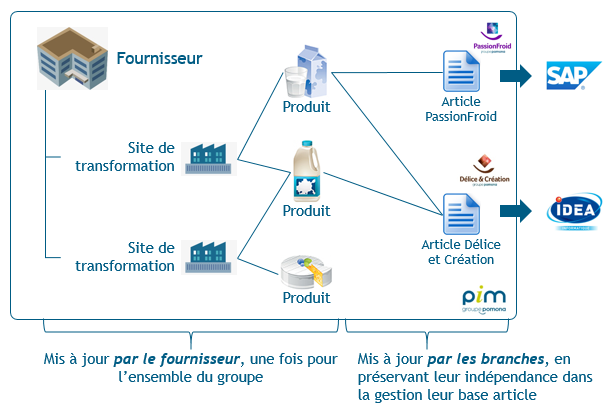
\includegraphics[width=\linewidth]{img/Produit article.png}
                \end{center}
                Dans cet exemple fictif, le type de conditionnement du lait n'a aucun impact sur les clients de la branche Délice et Création. Elle commercialise donc sous un même code article deux produits distincts.

                Pour des raisons de contrainte de conservation, la branche PassionFroid a quant à elle choisit de ne commercialiser qu'un seul produit - en brique. Elle pourrait choisir d'ouvrir un nouveau code article pour le lait en bouteille (non représenté sur le schéma ci-dessus).
                \caption{La distinction entre produit et article}
                \label{fig:produit_article}
            \end{figure}          

            \subsection{Les contrôles}

            Il a été vu que le Groupe Pomona - dans sa qualité de distributeur - n'est pas en mesure de déterminer seul les informations produit sur les marchandises qu'il commercialise.
            Néanmoins, comme cela a été vu dans la section \mref{utilisation_info_produit}, il est nécessaire que les différentes entités du Groupe soient en possession d'une information produit fiable.
            Or, avoir des données de qualité nécessite des efforts de la part des métiers, en particulier lorsque le processus n'est pas entièrement porté en interne dans la société.
            \`{A} ce titre, plusieurs étapes de contrôle ont été définies dans le processus de gestion du référentiel de données produit et article :
            \begin{description}
                \item[lorsque le fournisseur a saisi les données produit :] la personne à l'origine de la demande de référencement (en général, un acheteur) doit contrôler la cohérence des données produit
                \item[lorsque le demandeur a demandé la création d'un article :]  le gestionnaire de référentiel valide à nouveau la cohérence des informations produit
                \item[après la création article, de manière asynchrone :] le service qualité contrôle par échantillonnage les données d'une partie des produits et articles qui ont été modifiés pendant une période.
            \end{description}
            Le retour d'expérience montre que ces contrôles, loin d'être redondants, sont nécessaires pour avoir une qualité de données acceptable.
            Ces processus de contrôle sont décrits à la \reffig{fig:processus_article}.

            \begin{figure}[htpb]
                \begin{center}
                \includegraphics[width=\linewidth]{img/Processus de création article.png}
                \end{center}
                \caption{Le processus de création article}
                \label{fig:processus_article}
            \end{figure}    

            Les contrôles effectués à chacune des étapes sont les suivants : 
            \begin{description}
                \item[contrôle de la complétude des données :] vérification que les données transmises comportent l'ensemble des données attendues
                \item[contrôle de cohérence entre les données :] vérification que les informations transmises sont cohérentes entre elles (ex : un allergène présent dans la liste d'ingrédients du produit a bien été signalé comme allergène par ailleurs)
                \item[contrôle de la cohérence avec les pièces jointes :] en plus de données structurées, les fournisseurs transmettent également des fichiers portant des informations produit (ex : l'étiquette produit ou le visuel de l'emballage). Ces pièces jointes sont décrites à la section \mref{pieces_jointes}. La personne en charge du contrôle vérifie que les données transmises sont cohérentes avec ces documents.
            \end{description}

        \section{Les outils informatiques associés}
        \label{outils_infos}

        Comme vu dans la description des branches du Groupe (voir section \mref{les_branches}), les outils informatiques ne sont pas tous les mêmes sur l'ensemble des branches.
        Ainsi, les outils utilisés pour la gestion de l'information produit ne sont pas les mêmes.

            \subsection{Les branches faiblement outillées}
            
            Les branches étrangères (Pomona Suisse, Pomona Iberia), spécialistes (Délice et Création, Saveurs d'Antoine) et la branche TerreAzur sont aujourd'hui faiblement outillées.
            Cela signifie que l'information produit est en général stockée uniquement sous la forme de fichiers (essentiellement les pièces jointes, décrites à la section \mref{pieces_jointes}).
            L'ensemble des échanges avec les fournisseurs se font par mail, et les articles sont créés directement dans les systèmes de gestion par les gestionnaires de référentiel.
            Les liens entre les articles et les informations produit ne sont pas matérialisés dans les systèmes informatiques.

            \subsection{Le GIP}
            \label{GIP}

            Le GIP (Gestion de l'Information Produit) est utilisé sur la branche PassionFroid.
            C'est un système de gestion de l'information produit qui est maintenant obsolescent et en cours de remplacement.
            Il a toutefois le mérite de permettre le stockage dans une application des données et des pièces jointes relatives aux produits, avec la possibilité d'accéder aux informations produit à partir des identifiants des articles.
            C'est ce système qui a permis de pouvoir alimenter les sites de e-commerce PassionFroid et \'{E}piSaveurs avec les informations produit.
            Il est toutefois ancien, et ne propose pas de fonctionnalité d'export en masse fiable.
            Il s'agit d'une application qui n'est pas ouverte aux utilisateurs externes au Groupe, et les échanges avec les fournisseurs passent donc par des échanges de mails.

            \subsection{Le PIM}
            \label{PIM}

            Le PIM (Product Information Management) est un système de gestion de l'information produit qui a été mis en production en mai 2019, pour la branche \'{E}piSaveurs.

                \subsubsection{Description générale de l'outil}

                C'est un système qui porte l'ensemble du processus de gestion de l'information produit, tel que décrit à la \reffig{fig:processus_article}.
                Il est accessible aux fournisseurs du Groupe, qui viennent directement mettre à disposition les données et les pièces jointes.
                Cet outil porte entre autres les fonctionnalités de contrôle des informations, comme illustré à la \reffig{fig:ecran_PIM}.

                \begin{figure}[htpb]
                    \begin{center}
                    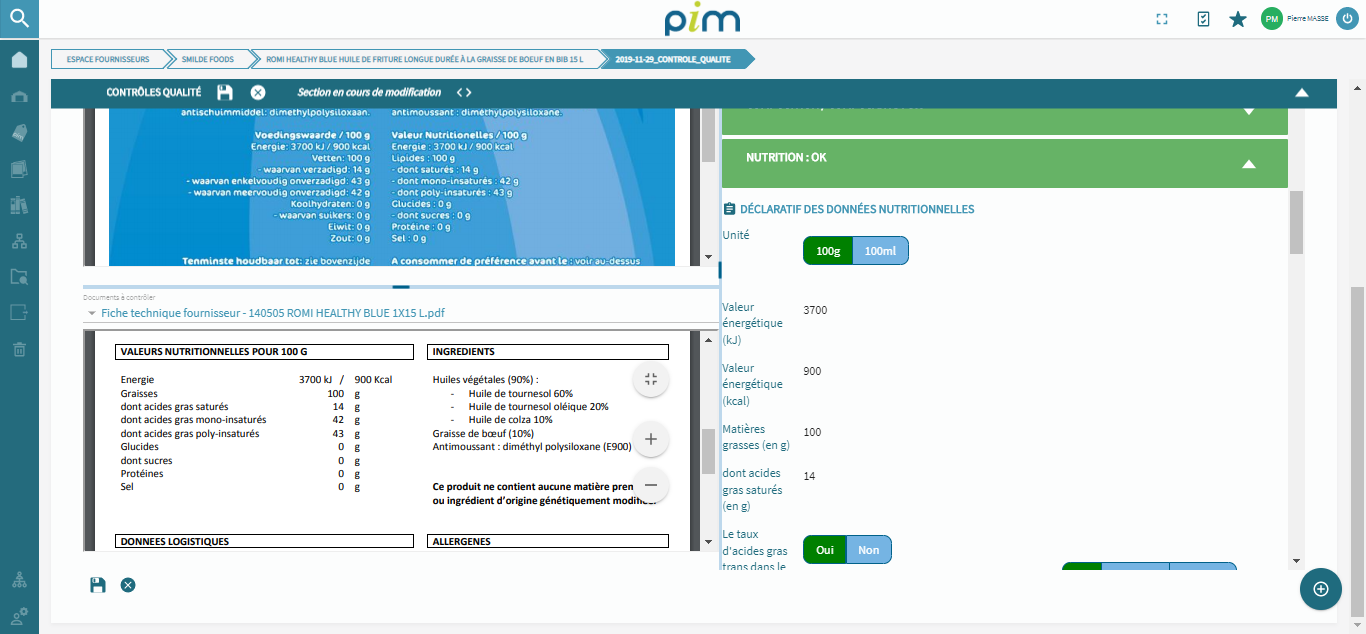
\includegraphics[width=\linewidth]{img/Ecran PIM.png}
                    \end{center}
                    Cette capture d'écran montre l'outil de contrôle des données produit. Sur la partie gauche, le contenu des pièces jointes est affiché (visuel de l'emballage en haut, fiche technique en bas), sur la droite les données qui ont été transmises par le fournisseur.
                    \caption{Une capture d'écran du PIM}
                    \label{fig:ecran_PIM}
                \end{figure} 

                \subsubsection{La GDSN}

                La GDSN (Global Data Synchronization Network) est un réseau d'échange de données produit entre industriels, distributeurs, restaurateurs, \dots
                Ce réseau est exploité par des opérateurs privés, mais le format et la chorégraphie des échanges a été standardisé par l'organisme de standardisation GS1.
                Son schéma de principe est décrit à la \reffig{fig:GDSN}.
                Sans rentrer dans le détail, au sein du Groupe Pomona l'utilisation qui en est faite est de récupérer les informations depuis ce réseau d'échange, afin de préalimenter les données produit pour les fournisseurs.
                Cette foncitonnalité permet de faire gagner du temps aux fournisseurs pour leur éviter une partie de ressaisie, mais également de limiter les erreurs.
                Toutefois, cette fonctionnalité ne permet pas à elle seule de garantir une parfaite qualité de données.
                Il s'agit uniquement d'un \og tuyau \fg, si les données en entrée ne sont pas correctes, elles ne seront pas correctes en sortie.
                Pour aller plus loin dans la compréhension de ce réseau, il est possible de consulter les ressources mises en ligne par GS1~\cite{GDSN_GS1_FR}\cite{GDSN_GS1_GLOBAL}.

                \begin{figure}[htpb]
                    \begin{center}
                    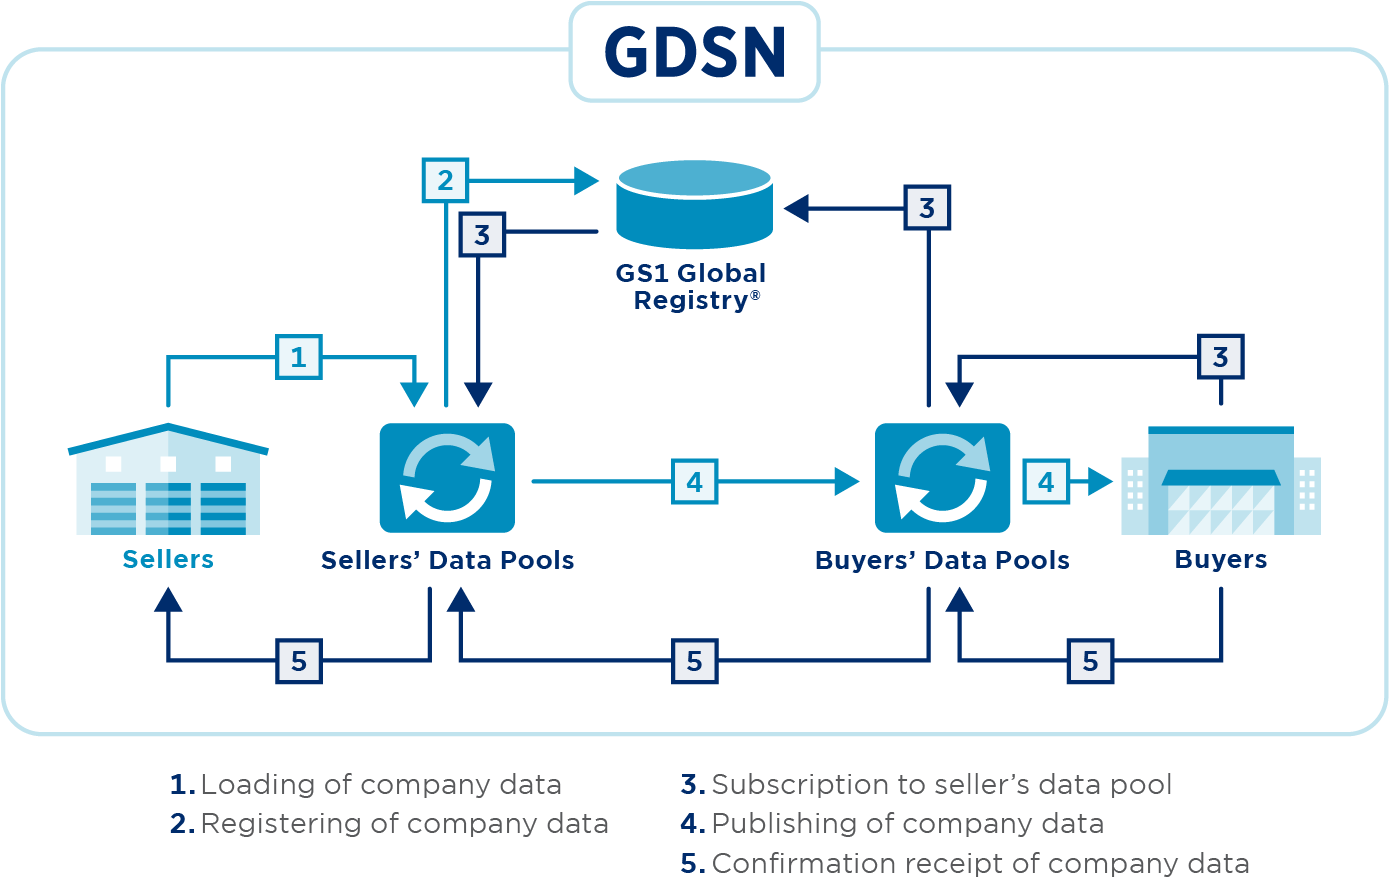
\includegraphics[width=\linewidth]{img/gdsn-schema.png}
                    \end{center}
                    \caption{Schéma de principe de la GDSN}
                    \label{fig:GDSN}
                \end{figure}                 
                
                \subsubsection{L'identification des objets dans le PIM}

                Un dernier point à connaître à propos du PIM, est la manière d'identifier l'ensemble des objets en son sein.
                Chaque objet géré (ainsi que toute version archivée) porte un identifiant unique, nommé \emph{uid} qui est totalement univoque.
                Pour la suite, on se basera sur ces uid pour faire référence à des produits stockés dans le PIM.
                Une illustration est présentée à la \reffig{fig:uid}.

                \begin{figure}[htpb]
                    \begin{center}
                    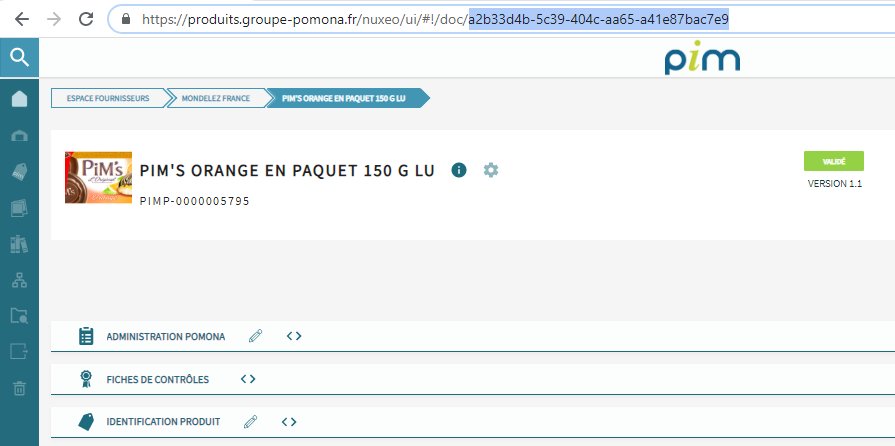
\includegraphics[width=\linewidth]{img/uid.png}
                    \end{center}
                    L'uid du produit affiché est mis en évidence dans l'url
                    \caption{L'uid d'un produit}
                    \label{fig:uid}
                \end{figure}                 

                \subsubsection{Les API}

                Un des aspects intéressants du PIM pour l'exploitation en masse des données produit, est qu'il expose des API permettant d'aller requéter l'ensemble de son contenu.
                Cela concerne à la fois les données dites structurées, mais également les pièces jointes.
                Cela rend les données produit de la branche \'{E}piSaveurs bien plus simplement accessibles que celles des autres branches.

\part{Les données}
    \chapter{Le périmètre produit}
    \label{perimetre_produit}
        \section{Accessibilité de la donnée en fonction des branches}

        Comme vu à la section \mref{outils_infos}, les systèmes d'information associés à la gestion de l'information produit offrent des niveaux d'accès hétérogènes à la donnée produit.
        Le récapitulatif par branche est le suivant : 
        \begin{description}
            \item[\'{E}piSaveurs :] on peut simplement accéder à l'ensemble des données produit, structurées, non structurées (i.e. textes longs) et pièces jointes
            \item[PassionFroid :] on a uniquement la possibilité d'exporter manuellement les données structurées articles depuis le système de gestion SAP.
            Elles permettent de produire quelques analyses quantitatives.
            Il est difficile de faire des exports en masse de l'outil de gestion de l'information produit GIP (cf. section \mref{GIP}).
            \item[TerreAzur :] idem PassionFroid, si ce n'est qu'en plus le système GIP n'est pas utilisé au sein de cette branche.
            \item[Délice et Création :] le système d'information ne permet pas d'exporter les données et donc de produire des indicateurs détaillés. On peut toutefois avoir des informations quantitatives de la part des opérationnels.
            \item[Saveurs d'Antoine :] idem Délice et Création
            \item[Pomona Suisse :] la branche est en cours de structuration, et les référentiels articles ne sont pas partagés entre les succursales. Il n'est pas possible d'obtenir d'information quantitative sur ces données.
            \item[Pomona Iberia :] idem Pomona Suisse
        \end{description}

        Pour les analyses quantitatives, on pourra se baser sur des extractions uniquement pour les branches RHD (\'{E}piSaveurs, PassionFroid, TerreAzur).
        L'ensemble des analyses portant sur les branches RHD sont produites sur la base d'extractions de leur système de gestion SAP.

        \section{Analyses quantitatives}
            \subsection{Comparatifs entre les branches}

                Les graphes de cette section ont été produits via le code présenté en annexe, au chapitre \mref{code:analyse_quantitative}.
                Les données pour les branches spécialistes (Délice et Création et Saveurs d'Antoine) sont issues d'informations fournies par le métier, hors système.


                En termes de volumétrie article (cf. \reffig{fig:volumetrie_article}, c'est TerreAzur qui possède le référentiel le plus étendu (environ 62 000 articles de marchandises actifs).
                Cela s'explique par le fait que cette branche commercialise essentiellement des produits bruts, non-préemballés (ex : des cagettes de fruits ou de légumes).
                Or, ces produits ne sont pas clairement identifiés, par exemple par un GTIN.
                Au démarrage de cette branche, afin de limiter la charge sur les gestionnaires de référentiels, le parti a été pris de créer en avance de phase l'ensemble des articles susceptibles d'être commercialisés.
                Cela s'est traduit par la création d'un grand nombre d'articles, du fait de l'application \og brutale \fg de la combinatoire des différents critères pouvant définir un produit.
                Un exemple (fictif) serait, sur les pommes : 
                \begin{itemize}
                    \item 8 variétés possibles (Gala, Golden, \dots)
                    \item 4 calibres possibles
                    \item 6 conditionnements possibles (plateau 6kg, plateau 4,5kg, \dots)
                    \item 2 catégories (I, II)
                    \item 8 origines (France, Espagne, \dots)
                \end{itemize}
                ce qui donne un total de 3072 articles uniquement sur cette gamme de produits.

                Viennent ensuite PassionFroid, et \'{E}piSaveurs, qui sont les autres \og grosses \fg branches historiques du Groupe.


                \begin{figure}[htbp]\CenterFloatBoxes
                    \begin{floatrow}
                    \ffigbox{%
                        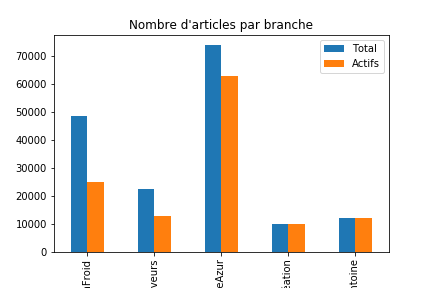
\includegraphics[width=200pt]{img/Articles par branche.png}%
                    }{%
                      \caption{Volumétrie article par branche}%
                      \label{fig:volumetrie_article}%
                    }
                    \capbtabbox[][][c]{%
                        \begin{tabular}{lccc}
\toprule
{} &  Total &  Actifs &  Marchandises \\
\textbf{Branche           } &        &         &               \\
\midrule
\textbf{PassionFroid      } &  48478 &   24898 &         24554 \\
\textbf{EpiSaveurs        } &  22498 &   12798 &         12241 \\
\textbf{TerreAzur         } &  73804 &   62789 &         62710 \\
\textbf{Délice et Création} &  10000 &       - &             - \\
\textbf{Saveurs d'Antoine } &  12000 &       - &             - \\
\bottomrule
\end{tabular}
%
                    }{%
                      \caption{Volumétrie article par branche}%
                    }
                    \end{floatrow}
                \end{figure}
                    
                Une analyse du recouvrement des référentiels montre que dans l'esemble, les branches ne travaillent pas les mêmes articles (cf. \reffig{fig:venn_article}).
                PassionFroid commercialise certains produits des branches \'{E}piSaveurs et TerreAzur, mais cela s'explique par une petite entité luxembourgeoise qui travaille des produits de tout type de stockage.
                Une réserve toutefois par rapport à cette analyse de recouvrement produit : elle sous-estime vraisemblablement lesdits recouvrements, dans la mesure où la présence de doublons n'est pas prise en compte.

                \begin{figure}[htbp]
                    \begin{center}
                    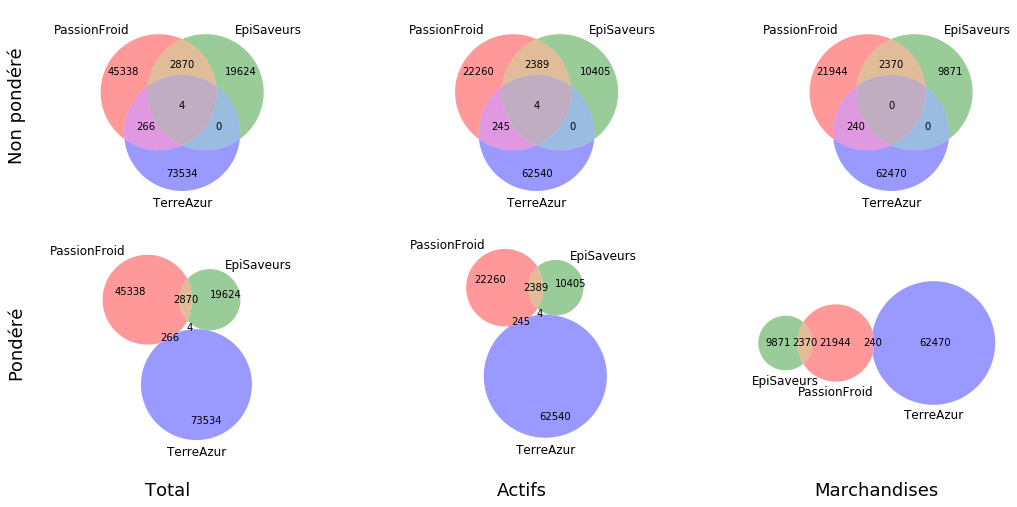
\includegraphics[width=\linewidth]{img/Diagrammes de Venn articles.png}
                    \end{center}
                    \caption{Recouvrements entre branches RHD}
                    \label{fig:venn_article}
                \end{figure}       

            \subsection{Les grands types de produits}

            Comme montré à la \reffig{fig:repart_art_categ}, on voit bien que les données ta race.

            \begin{figure}[htbp]
                \begin{center}
                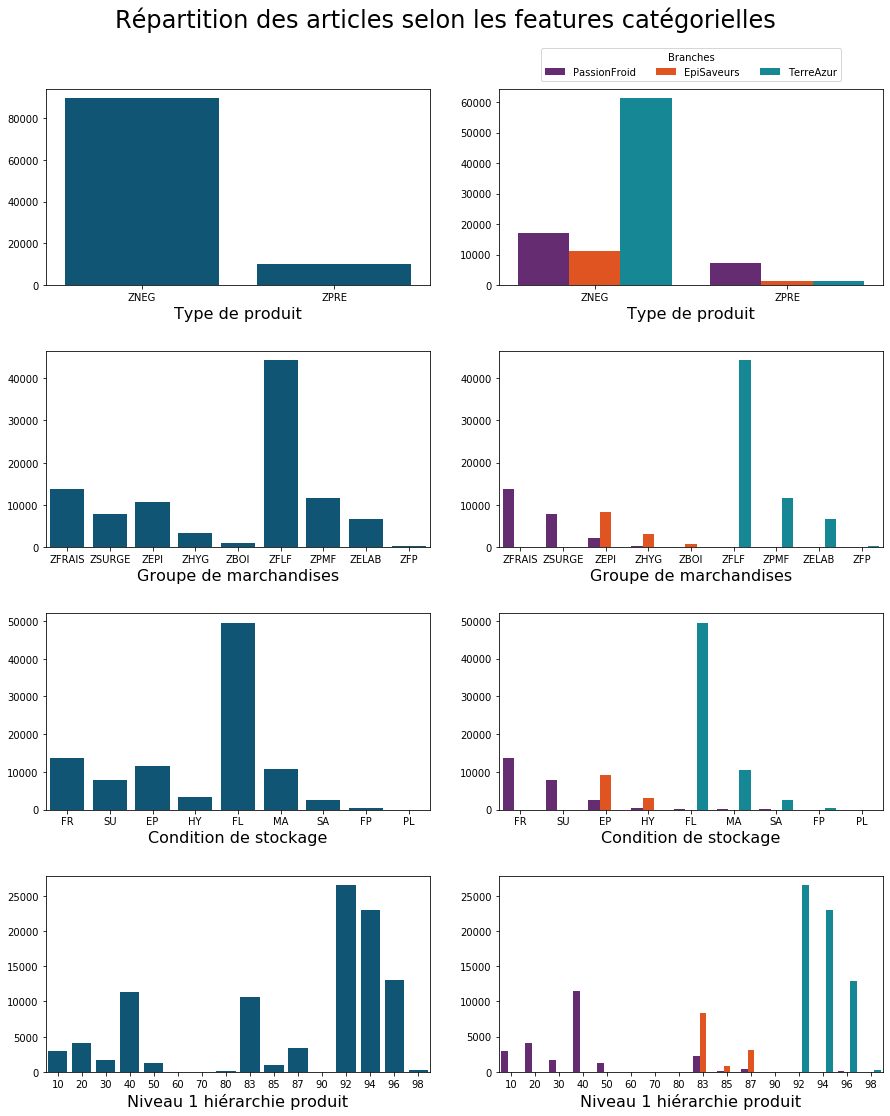
\includegraphics[width=\linewidth]{img/Repartition articles categories.png}
                \end{center}
                \caption{Répartition des articles en fonction des variable catégorielles}
                \label{fig:repart_art_categ}
            \end{figure}

            Repartition articles catégories
            Focus sur les branches Jupiter.
            Par type d'article / groupe de marchandises / groupe d'article, en retirant les articles inactifs. Toujours avec la vision article et produit (FIA).

            Ajout aussi du niveau 1 de la hiérarchie produit. Voir la possibilité de faire une représentation en 2D (type art / hiérarchie). Avec genre une heatmap qui montre que certaines de ces variables catégorielles sont en fait très très liées.

    \chapter{Les données utilisables}
        \large
        Comme vu au chapitre \mref{perimetre_produit}, les données produit ne sont simplement accessibles que pour la branche \'{E}piSaveurs.
        On se focalisera donc sur cette branche pour la suite de cette étude.
        \normalsize

        \section{Données structurées}

        Les données dites structurées sont l'ensemble des données qui peuvent prendre leurs valeurs dans un domaine restreint.
        Par exemple, ce sont les données booléennes, les choix issus de listes déroulantes, les valeurs numériques\dots
        Les principales données structurées pour les produits alimentaires dans le PIM sont : 
        \begin{description}
            \item[le code du produit :] calculé par le système
            \item[le fournisseur :] référence croisée vers le code du fournisseur
            \item[le type de produit :] épicerie, boisson alcoolisée, hygiène, chimie, boisson non-alcoolisée
            \item[le type d'unité de base :] paquet, boîte, sachet, rouleau, bouteille, pot, \dots
            \item[le GTIN du produit :] identifiant numérique unique, utilisé entre autres pour l'étiquetage sous forme de code à barres~\cite{GS1_GTIN}
            \item[les poids :] brut, net, net égoutté (pour les conserves)
            \item[le volume :] pour les produits liquides
            \item[les durées de vie :] le type (Date Limite de Consommation ou Date de Durabilité Minimale) et la durée (totale à fin de production, garantie à livraison)
            \item[les modes de conservation avant/après ouverture :] à température ambiante, au réfrigérateur puis à consommer sous 2 jours, \dots
            \item[les labels :] le(s) label(s) s'appliquant au produit (cf. section \ref{labels} page \pageref{labels})
            \item[les régimes particuliers :] Halal, Casher, Sans porc, Végétarien, Végétalien, \dots
            \item[les caractéristiques spéciales :] sans OGM, non traité par ionisation
            \item[la présence d'allergènes :] le niveau de présence de chacun des 14 allergènes réglementés (cf. section \ref{composition} page \pageref{composition})
            \item[les matières grasses utilisées :] palme, beurre, coco, tournesol, palmiste, \dots
            \item[les additifs présents :] les codes Exxx et les fonctions des additifs mis en oeuvre~\cite{additifs_regl_eu}\cite{additifs_wiki}
            \item[les données nutritionnelles obligatoires :] pour 100g ou 100mL, valeur énergétique (en kJ et kcal), matières grasses, dont acides gras saturés, Glucides, dont sucres simples, Fibres, Protéines, simplement
            \item[les données nutritionnelles facultatives :] vitamines, minéraux, omégas, \dots
            \item[les allégations nutritionnelles :] riche en, faible en, sans,\dots associé à un nutriment défini dans les 2 points précédents
            \item[le nutriscore :] note allant de A à E, définie dans la loi Santé de janvier 2016
            \item[le taux de TVA :] un des quatre taux définis dans la réglementation française
            \item[le code nomenclature douanière :] code identifiant les marchandises défini par les douanes pour la Déclaration d'\'{E}change de Biens~\cite{notions_DEB}
            \item[le pays d'origine pour la DEB :] le pays d'origine à déclarer dans la Déclaration d'\'{E}change de Biens~\cite{notions_DEB}
            \item[] 
        \end{description}
        
        
        \section{Données non structurées}
        
        Les listes d'ingrédients juste une liste ordonnées d'ingrédients triés par ordre décroissant de quantité mise en oeuvre.

        Parfois détaillé par phase, mais en général déconseillé.
        \section{Pièces jointes}
            \label{pieces_jointes}

            Dans chacune des sections, mentionner la volumétrie de données accessibles (avec les facettes migration, statuts, \& compagnie) et tout

            \subsection{Fiches techniques fournisseur}
            \subsection{\'{E}tiquettes produit}
            \subsection{Fiches logistiques fournisseur}
            \subsection{Fiches techniques et argumentaires Pomona}
        \section{Récapitulatif de la complétude des données}

        Mettre ici un ou plusieurs tableaux récapitulatifs illustrant les données possédées quantitativement.

        \section{Analyse qualitative des données}
        
        Montrer qu'un sondage basique fait que la qualité actuelle est perfectible

        Mettre également la distribution numérique des produits par fournisseur et insister sur la difficulté posée par de multiples formats

        Dire ici qu'il y a finalement beaucoup de pdf qui possèdent des textes extractibles vs. uniquement des images.

        \section{Les données \og manuellement étiquetées \fg}

        Montrer comment elles ont été produites

        Expliciter les règles de gestion qui ont été listées pendant l'étiquetage manuel

        Evaluer la cohérence entre étiquettes manuelles et contenu du PIM


\part{Les objectifs de ce projet}
    \chapter{Les cas d'usage}
        \section{Objectifs : Qualité et productivité}
        Comme présenté précédemment, 1 on dépense de l'énergie, et 2 on a une qualité de données qui est perfectible.
        Un traitement automatique des documents mis à disposition permettrait de décharger les personnes qui interviennent dans le processus (fournisseurs, acheteurs, gestionnaires de référentiels, ingénieurs qualité) et de garantir une meilleure pertinence de l'information produit.

        \section{La préalimentation d'information}
        Préalimenter les informations, sous réserve d'avoir un outil suffisamment fiable, permettrait de faire gagner du temps aux fournisseurs.
        Trois obstacles:
        \begin{itemize}
            \item cela n'a d'intérêt que si le système est capable de produire de l'information structurée avec une fiabilité élevée (par exemple, 80\% de données correctes serait un minimum)
            \item cela entre en concurrence directe avec le système GDSN présenté au paragraphe portant le même nom à la section \mref{GDSN}.
            Or, ce système est justement spécialement conçu pour faire transiter les informations produit des fournisseurs aux distributeurs, avec une standardisation des échanges
            \item cela apporte l'essentiel de la valeur aux fournisseurs, mais pas au Groupe
        \end{itemize}

        \section{Le contrôle des informations transmises}

        Cf. le schéma présenté à la \reffig{fig:processus_article}.
        Plus le taux de détection des erreurs est élevé, et plus les erreurs sont détectées tôt, mieux c'est : 
        \begin{itemize}
            \item la qualité des données s'en trouve évidemment améliorée
            \item le processus est plus court en temps, en évitant les aller-retours
            \item on décharge l'ensemble des acteurs, en limitant la
             
        \end{itemize} 

            \subsection{Le contrôle à la saisie fournisseur}
            Si on alerte le fournisseur au moment où il saisit, on peut dès le début du processus éviter une erreur.
            Cela pourrait avoir lieu quand il soumet ses donner, on fait tourner un traitement et on remonte des avertissements dans l'IHM du PIM.

            \subsection{L'aide aux vérifications Pomona}
            Lors des contrôles, on pourrait également remonter les incohérences détectées entre pièces jointes et données à contrôler.

            \subsection{Les contrôles en masse asynchrones}
            Enfin, il pourrait être pertinent de faire tourner de manière asynchrone des contrôles de qualité de données sur l'ensemble de la base.
            TODO : détailler un peu le pourquoi c'est nécessaire (exemple du champ acides gras trans), et un des point difficile : acquittement des avertissements non pertinents.

    \chapter{Le choix du cas d'usage}

        \section{La représentation dominante des fiches techniques}
        On a beaucoup de fiches techniques, pas beaucoup d'étiquettes ou de fiches logistiques (cf. la table qui va bien.)
        On va donc plutôt dans un premier temps tenter de travailler avec les fiches techniques.

        \section{Les multiples formats et le besoin de \og spatialisation \fg}
        \label{formats_spatialisation}

        Chaque fournisseur décide évidemment du format de document qu'il souhaite produire.
        On a donc beaucoup de formats différents, et un Pareto finalement trop \og mou \fg pour envisager de construire des templates pour récupérer les informations automatiquement (cf. \reffig{fig:rappel_pdt_par_frn}).
    
        \section{Les informations \og spatialisées \fg}
        Les données que l'on souhaite récupérer sont globalement de 3 types : 
        \begin{itemize}
            \item données de composition
            \item données nutritionnelles
            \item données logistiques
        \end{itemize}

        Comme vu dans la section \mref{fiches_techniques}, un grand nombre d'informations sont spatialisées.
        Par exemple, la représentation des données nutritionnelles se fait régulièrement sous forme de tableau.
        Or, c'est un peu compliqué à interpréter, car il fut réussir à interpréter un tableau, et à en sortir des couples de clé / valeur.

        \section{La complexité dans la représentation des données logistiques}

        Les données logistiques sont souvent difficile à interpréter pour un humain, donc cette activité peut paraître difficile à déléguer à une machine.
        Mettre 2-3 exemples.

        \section{L'identification d'une liste d'ingrédient par son contenu}

        Il est possible de dire si un texte est une liste d'ingrédients, juste en lisant ce texte.
        Par exemple, \og 14g \fg peut être une quantité de glucides, de lipides, le poids d'une pièce unitaire, \dots
        Mais un texte tel quel <mettre ici un exemple> a de forte chance d'être le contenu d'une liste d'ingrédients.

        \section{Conclusion quant au choix du cas d'usage}

        Tant la préalimentation, que l'aide au contrôle des données seraient faisable d'un point de vue technique.
        Il suffirait pour cela de publier un service, qui fonctionnerait de la manière suivante : 
        \begin{itemize}
            \item le PIM appelle le service, avec un message contenant l'uid du produit à contrôler ou préalimenter
            \item le serveur récupère du PIM les données nécessaires au contrôle ou à la préalimentation
            \item en retour, il renvoie au PIM soit l'état du contrôle (OK, erreur, avertissement, avec les précisions nécessaires), soit les données telles qu'elles doivent être préalimentées
            \item le PIM, sur la base de ce retour, affiche le résultat du contrôle ou bien alimente les données et les présente à l'utilisateur
        \end{itemize}

        \emphbox{Au vu des différentes contraintes listées dans ce document, on s'attachera à extraire \emph{les listes d'ingrédients} des produits \emph{alimentaires} de la branche \emph{EpiSaveurs} depuis \emph{les fiches techniques fournisseur}, en se basant sur \emph{le contenu textuel} de ces documents.}

\part{Construction du modèle}

    \chapter{Prototypage}
    \label{prototypes}

    \section{Premier prototype : modèle simple \og ouvert \fg}
        
        \subsection{Principes généraux}

            \begin{figure}[htbp]
                \begin{center}
                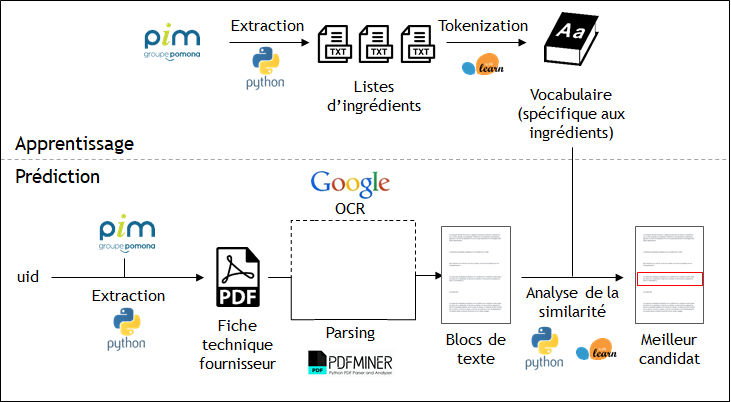
\includegraphics[width=0.9\linewidth]{img/open_model.png}
                \end{center}
                \caption{Schéma de principe du \og modèle ouvert \fg}
                \label{fig:open_model}
            \end{figure}     

            Le fonctionnement global de ce premier modèle (présenté à la \reffig{fig:open_model}) ne respecte pas les principes du machine learning.
            Il permet juste d'éprouver la méthode pressentie, ainsi que de se faire une idée de l'efficacité d'un modèle de ce type.
            En effet, même si on utilise des fonctionnalités d'extraction de features depuis des textes classiques dans des modèles de machine learning, il manque une partie de mesure de la performance, indispensable pour pouvoir évaluer et améliorer la pertinence du modèle.
            Les illustrations de ce chapitre sont issues du notebook présenté en annexe \mref{code:open_model}, et le code des classes utilisées (IngredientExtractor et PIMIngredientExtractor) est inclus dans le module pimest, en annexe \mref{code:pimest}.

            La classe PIMIngredientExtractor est juste un habillage du CountVectorizer de la bibliothèque scikit-learn et du Requester construit dans le module pimapi, permettant d'aller récupérer les données du PIM.
            Ce modèle met en application les principes du \og Bag Of Words \fg \cite{bag_of_words_wiki}, à savoir que :
            \begin{itemize}
                \item un vocabulaire est établi à partir de l'ensemble des différents mots du corpus de listes d'ingrédients
                \item chaque liste d'ingrédients est transformée en un vecteur de nombres entiers qui a la même longueur que le vocabulaire, ou chaque entier est le compte du nombre d'occurence du mot dans le vocabulaire
            \end{itemize}

            Ce modèle n'utilise pas les données étiquetées manuellement (présentées à la section \mref{manually_labelled_data}), mais se base simplement sur les listes d'ingrédients du PIM.
            L'hypothèse qui est faite avec ce modèle est la suivante : bien que non parfaitement en qualité (i.e. exactement identiques au contenu des pièces jointes, cf. la comparaison entre la ground truth et le contenu du PIM en section \mref{ingredient_comparison}), les listes d'ingrédients du PIM sont des textes dont le contenu est très similaire à une liste d'ingrédients.
            Un survol rapide de quelques exemples montre que cette hypothèse semble vérifiée (cf. \reftable{tbl:exemple_ingred}).

        \subsection{Entraînement}

            \subsubsection{Périmètre du set d'entraînement}
            
            Pour l'entraînement de ce modèle, on va uniquement se limiter aux produits d'épicerie ou de boissons non-alcoolisées.
            En effet, ce sont pour ces produits que la réglementation impose d'afficher en clair la composition aux consommateurs.
            On se limitera aussi aux produits qui portent une liste d'ingrédients, et qui sont \og En qualité \fg (cf. les définitions données à la section \mref{statuts} sur les statuts des produits).
            Sur les 13 000+ produits présents dans le PIM, environ 3 400 font partie du périmère et 9 800 en sont exclus.

            \subsubsection{Constitution du vocabulaire}

            La constitution du vocabulaire se fait de manière très basique : 
            \begin{itemize}
                \item les listes d'ingrédients sont mises en minuscules
                \item les mots sont ensuite séparés aux whitespaces (espaces, retours à la ligne, tabulations, \dots) et marques de ponctuation
            \end{itemize}
            Pour parvenir à ce résultat, on applique simplement la méthode fit de la classe CountVectorizer de la bibliothèque scikit-learn.
            Aucunes des autres fonctionnalités standard (retrait des accents, gestion des stopwords, prise en compte des ngrams) n'a été utilisée.
            Lors de cet apprentissage, le vocabulaire obtenu a une longueur de 2 500 mots environ, et les mots les plus fréquents sont (ces valeurs sont susceptibles de changer à la marge par rapport au notebook en annexe, avec les changements potentiels sur les données au sein du PIM):
            \begin{itemize}
                \item de     : 11419 occurences
                \item sucre  :  2057 occurences 
                \item sel    :  1669 occurences
                \item eau    :  1288 occurences
                \item acide  :  1241 occurences
                \item lait   :  1215 occurences
                \item huile  :  1214 occurences
                \item poudre :  1100 occurences
                \item en     :   962 occurences
                \item arôme  :   938 occurences
            \end{itemize}
            Les stopwords 'de' et 'en' apparaissent dans les mots les plus fréquents.
        
        \subsection{Prédiction}
            
            \subsubsection{Parsing des fiches techniques}

                Les fiches techniques sont extraites sous formes de binaires depuis de le PIM via des appels API.
                On utilise ensuite la bibliothèque PDFMiner.six pour récupérer le texte de la fiche technique sous forme d'un long string.
                Cette étape fait appel à la méthode statique PDFDecoder.content du module pimpdf, présenté en annexe \mref{code:pimpdf}.
                On découpe ensuite ce long string en une liste de strings plus court, en considérant comme séparateur la présence de deux retours à la ligne consécutifs.
                Ce choix de séparateur a été fait car les textes produits par PDFMiner.six portent des retours à la ligne à la fin de chaque ligne typographiée, même si la phrase continue sur la ligne suivante.
                Cette étape fournit pour chaque fiche technique le texte contenu sous forme d'une liste de strings (les blocs de texte de la \reffig{fig:open_model}).

            \subsubsection{Sélection du meilleur candidat}
            \label{open_model_similarity}

                \paragraph{Principe}
                L'identification du meilleur candidat parmi les blocs de texte se fait de la manière suivante :
                \begin{itemize}
                    \item on calcule une similarité avec le vocabulaire des ingrédients pour chacun des blocs de texte
                    \item on retourne le bloc de texte avec la similarité la plus élevée
                \end{itemize}
                La formule de calcul de la similarité utilisée dans ce modèle a été trouvée par chance, mais elle donne des résultats plutôt encourageants.
                D'autres modes de calcul de la similarité seront présentés dans la suite de ce rapport.

                La formule de calcul de la similarité est :
                \[\frac{\text{Nombre de mots du candidat qui sont des ingrédients}}{\text{Norme euclidienne du vecteur du candidat}}\]
                
                Attention, la norme du vecteur du candidat s'entend \emph{indépendamment du vocabulaire des ingrédients}, c'est à dire que tous les mots comptent, y compris ceux n'appartenant pas au vocabulaire.

                \paragraph{Exemple}
                Si on illustre par un exemple fictif : imaginons que le vocabulaire des ingrédients soit composé des mots \emph{\og eau \fg, \og sucre \fg et \og farine \fg}.
                Le bloc de texte candidat est \emph{\og Sucre et farine sont biologiques. La farine est équitable.\fg}
                Si on vectorise ce bloc de texte \emph{sur son propre vocabulaire}, on obtient le vecteur suivant : 

                \bigskip
                \begin{minipage}{\textwidth}
                \captionsetup{type=table}
                \centering
                \begin{tabular}{cccccccc}
                    \toprule
                    sucre & et & farine & sont & biologiques & la & est & équitable \\
                    \midrule
                    1 & 1 & 2 & 1 & 1 & 1 & 1 & 1 \\
                    \bottomrule
                \end{tabular}
                \caption{Exemple de vectorisation d'un texte}
                \bigskip
                \end{minipage}                

                Sa norme euclidienne~\cite{norm_wiki} se calcule de la manière suivante (en notant $x_{i}$ le compte des mots) : 
                \[\sqrt{\sum_{i}^{} x_{i}^{2}} = \sqrt{1 + 1 + 4 + 1 + 1 + 1 + 1 + 1} \approx 3.317\]

                Le bloc contient 9 mots, dont 3 sont des ingrédients (\og farine \fg est mentionné deux fois). La similarité pour cet exemple vaut donc :
                \[\frac{3}{3.317} \approx 0.905\]
                \'{E}tant donné son mode de calcul, cette similarité peut tout à fait être supérieure à 1.

        \subsection{Illustration des résultats obtenus}
    
            \subsubsection{Périmètre du test}
            
            Pour éviter de surestimer la performance du modèle, on le fait tourner sur des produits n'ont pas fait partie du set d'entraînement.            
            Comme ce modèle ne permet de toute façon pas de fournir de résultats qui permettent de mesurer la performance, on ne le fera tourner que sur un échantillon réduit de produits, soit 5 d'entre eux.

            \subsubsection{Résultats}

            Les résultats obtenus sont les suivants :

                \begin{spacing}{1.0}
                \label{blocks_examples}
                {\scriptsize
                {\ttfamily 
                \begin{spverbatim}
Fetching data from PIM for uid d9b233a6-b455-4af6-afb4-623f1f7f62a6...
Done
----------------------------------------------------------
Ingredient list from PIM is :

Ingrédients: Huile de tournesol, oignon, curry (11,2%) (ail, coriandre, curcuma, gingembre, paprika, poivre, cumin, poivre de Cayenne, fenouil, cardamome, noix de muscade, canelle, clous de girofle, safran), pomme, sel, exhausteur de goût (glutamate de sodium), sucre, huile de colza totalement hydrogénée, extrait de levure, ail.
----------------------------------------------------------
Downloading content of technical datasheet file...
Done!
----------------------------------------------------------
Parsing content of technical datasheet file...
Done!
----------------------------------------------------------
Ingredient list extracted from technical datasheet:

Liste d’ingrédients : Huile de tournesol, oignon, curry (11,2%) (ail, coriandre, curcuma, gingembre, paprika, poivre, cumin,
poivre de Cayenne, fenouil, cardamome, noix de muscade, canelle, clous de girofle, safran), pomme, sel, exhausteur de goût
(glutamate de sodium), sucre, huile de colza totalement hydrogénée, extrait de levure, ail
----------------------------------------------------------

=======================================================================
=======================================================================
Fetching data from PIM for uid 5666235b-9e78-44f2-8e0e-1de53f88fe04...
Done
----------------------------------------------------------
Ingredient list from PIM is :

Ingrédients : Sucre, Gomme base, Sirop de glucose, Arômes, Humectant (E422), Antioxydant (E321), Colorant (E141).
----------------------------------------------------------
Downloading content of technical datasheet file...
Done!
----------------------------------------------------------
Parsing content of technical datasheet file...
Done!
----------------------------------------------------------
Ingredient list extracted from technical datasheet:

INGRÉDIENTS : Sucre, Gomme base, Sirop de glucose, Arômes, Humectant (E422), 
Antioxydant (E321), Colorant (E141).
----------------------------------------------------------

=======================================================================
=======================================================================

Fetching data from PIM for uid 6e976147-adeb-4d2d-925a-cb7c58c111a2...
Done
----------------------------------------------------------
Ingredient list from PIM is :

Maltodextrine, amidon de maïs, sel, farine de BLE, colorant : caramel ordinaire ; arômes (BLE,CELERI), huile de palme, épaississant : gomme guar ; oignon, fécule de pomme de terre, extrait de levure, jus de cuisson de viande de boeuf (0,9%), acidifiant : acide citrique ; extrait de vin blanc, extraits d'ail, de thym et de poivre. Peut contenir : LAIT, OEUF.
----------------------------------------------------------
Downloading content of technical datasheet file...
Done!
----------------------------------------------------------
Parsing content of technical datasheet file...
Done!
----------------------------------------------------------
Ingredient list extracted from technical datasheet:

Maltodextrine, amidon de maïs, sel, farine de blé, colorant : caramel ordinaire ; arômes (blé,céleri), huile de palme, épaississant : gomme guar ; oignon, fécule 
de pomme de terre, extrait de levure, jus de cuisson de viande de bœuf (0,9%), acidifiant : acide citrique ; extrait de vin blanc, extraits d'ail, de thym et de poivre. 
Peut contenir : lait, œuf.

----------------------------------------------------------

=======================================================================
=======================================================================

Fetching data from PIM for uid db449562-d16d-4f72-b7a5-c0d487bc8206...
Done
----------------------------------------------------------
Ingredient list from PIM is :

Huile d'ARACHIDE

----------------------------------------------------------
Downloading content of technical datasheet file...
Done!
----------------------------------------------------------
Parsing content of technical datasheet file...
Done!
----------------------------------------------------------
Ingredient list extracted from technical datasheet:

*Selon le règlement UE n°1259-2011 / In accordance with regulation UE n°1259-2011  
    
    
CARACTERISTIQUES MICROBIOLOGIQUES 
    
L’huile étant un milieu anhydre, tout développement bactérien est impossible (cf. ouvrage de 
référence  dans  ce  domaine  "La  qualité  microbiologique  des  aliments"  CNERMA-CNRS 
coordonné par Jean-louis Jouve). 
    
ORIGINES/ ORIGIN 
    
- Amérique du Sud majoritairement 
- Afrique de l’Ouest 
    
AUTRES INFORMATIONS 
    

----------------------------------------------------------

=======================================================================
=======================================================================

Fetching data from PIM for uid f2af54a2-6820-4f1b-99e7-d6e64642bdf3...
Done
----------------------------------------------------------
Ingredient list from PIM is :

None

----------------------------------------------------------
Downloading content of technical datasheet file...
Done!
----------------------------------------------------------
Parsing content of technical datasheet file...
Done!
----------------------------------------------------------
Ingredient list extracted from technical datasheet:

mini 16,56 ( - 10 % )

----------------------------------------------------------

=======================================================================
=======================================================================  
                \end{spverbatim}
                }
                }
                \end{spacing}

            \subsubsection{Pistes d'améliorations identifiées}

            En plus de la mesure de la performance, qui est indispensable avant de pouvoir procéder à des ajustements, les pistes identifiées à sont les suivantes :
            \begin{itemize}
                \item Faire un découpage plus élaboré du texte des pièces jointes en blocs, potentiellement avec des expressions régulières
                \item Essayer d'autres manières de vectoriser les textes (utiliser un comptage de mots binaire : présence/absence, calculer l'inverse document frequency, \dots)
                \item Essayer une autre manière de calculer la similarité
                \item Utiliser des fonctions plus élaborées de text preprocessing (retrait des stopwords, \dots)
            \end{itemize}

    \section{Second prototype : industrialisation}

            % REPRENDRE LA RELECTURE ICI

    L'objectif de ce second prototype est de permettre est d'industrialiser un peu le code afin : 
    \begin{itemize}
        \item d'être en mesure inspecter les résultats obtenus et pouvoir donner des explications sur la réponse donnée par le modèle
        \item de pouvoir utiliser des fonctionnalités de mesure de la performance du modèle
        \item d'être en mesure de faire varier les paramètres du modèle en vue de l'optimiser
    \end{itemize}
    Comme présenté à la section \mref{ingredient_comparison} relative à la comparaison entre les données du PIM et celles récupérées lors de l'étiquetage, il y a un grand nombre d'écarts.
    Or, si on entraîne le modèle et qu'on mesure sa performance sur des données de mauvaise qualité, on aura de mauvais résultats.
    Ce second modèle se basera sur les données manuellement étiquetées, afin d'avoir une base de comparaison dans la mesure de la performance.
    Le fonctionnement de ce modèle est présentés à la \reffig{fig:ground_truth_model}.
    La méthodologie utilisée à cette partie est présentée dans le notebook \og Modèle basé sur les données manuellement étiquetées \fg en annexe \mref{code:gt_based_model}.
    Les différents transformateurs et estimateurs spécifiques sont définis dans le module pimest, inclu en annexe \mref{code:pimest}.
    
    \begin{figure}[htbp]
        \begin{center}
        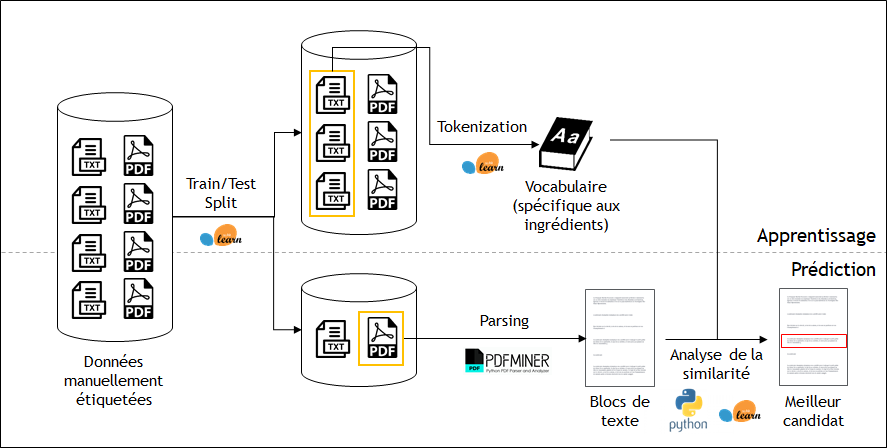
\includegraphics[width=0.9\linewidth]{img/ground_truth_model.png}
        \end{center}
        \caption{Schéma de principe du modèle basé sur les données étiquetées}
        \label{fig:ground_truth_model}
    \end{figure}     

        \subsection{Chargement des données manuellement étiquetées}

        La toute première étape est la constution d'un dataframe contenant : 
        \begin{itemize}
            \item les uid pour indexer les produits
            \item les listes d'ingrédients manuellement étiquetées depuis les fiches techniques
            \item le contenu de chacune des fiches techniques au format texte
        \end{itemize}
        On commence par charger les données du fichier csv contenant les uid et les listes d'ingrédients.
        Ensuite, un pipeline scikit learn d'acquisition des données est lancé.
        Il s'agit de 4 transformateurs en série, qui effectuent les travaux suivants :
        \begin{itemize}
            \item construction du chemin pointant vers les fiches techniques (sur la base des uid)
            \item construction d'une feature contenant les données des fichiers, en binaire
            \item construction du texte complet de la fiche technique (en se basant sur la library pdfminer.six)
        \end{itemize}
        Le résultat du lancement de ce pipeline est présenté à la \reftable{tbl:mod_GT_fulltexts}.

        {\renewcommand{\arraystretch}{1.5}%
        \begin{table}[htbp]
            \begin{center}
            {\scriptsize
            \begin{tabular}{p{\linewidth}}
\toprule
                                                                                                                                                                                                                                                                                                                                                                                                                                                                                                                                                                                                                                                                                                                                                                                                                                                                                                                                                                                                                                    text \\
\midrule
 NESCAFÉ® SPÉCIAL FILTRE\textbackslash n\textbackslash nDose individuelle de 2 g\textbackslash nTechnologie micro-grains\textbackslash n\textbackslash nCODE EAN (UC)\textbackslash n\textbackslash n3033710076017\textbackslash n\textbackslash nDENOMINATION LEGALE DU PRODUIT\textbackslash n\textbackslash nDESCRIPTION DU PRODUIT\textbackslash n\textbackslash nCafé instantané et café torréfié moulu.\textbackslash n\textbackslash nUne dominante Arabica pour l'arôme et une pointe de Robusta pour le \textbackslash ncorsé, associés à une torréfaction légère pour un café équilibré et peu \textbackslash namer.\textbackslash nSachet dose pour une tasse.\textbackslash n\textbackslash nDOSAGE PRECONISÉ\textbackslash n\textbackslash nMODE OPERATOIRE\textbackslash n\textbackslash nPour obtenir\textbackslash n\textbackslash n1 café Court (DA)\textbackslash n\textbackslash n1 café Long (DA)\textbackslash n\textbackslash nEau\textbackslash n\textbackslash n7\textbackslash n\textbackslash n12\textbackslash n\textbackslash ncl\textbackslash n\textbackslash ncl\textbackslash n\textbackslash nNESCAFÉ®\textbackslash n\textbackslash n SPÉCIAL FILTRE\textbackslash n\textbackslash n2\textbackslash n\textbackslash n2\textbackslash n\textbackslash ng\textbackslash n\textbackslash ng\textbackslash n\textbackslash nA reconstituer avec de l'eau. \textbackslash nTempérature de l'eau : 75°C\textbackslash nPour une qualité optimale, utilisez de l'eau filtrée.\textbackslash n\textbackslash nIngrédients : Café instantané, café torrefié moulu (3\%).\textbackslash n\textbackslash nINGRÉDIENTS\textbackslash n\textbackslash nPROFIL GUSTATIF\textbackslash n\textbackslash nIntensité\textbackslash n\textbackslash nConditionné sous atmosphère protectrice.\textbackslash n\textbackslash nENGAGEMENT QUALITÉ\textbackslash n\textbackslash n- NESTLÉ a un système de management de la qualité, le NMS (NESTLÉ \textbackslash nManagement System), en cohérence avec les systèmes ISO 9001 ... \\
 LENTILLES BLONDES 4mm\textbackslash n\textbackslash nRéférence PQG007-3.22.1\textbackslash nVersion\textbackslash nDate d'application :\textbackslash nPage 1/2\textbackslash n\textbackslash nG\textbackslash n\textbackslash n15/10/2019\textbackslash n\textbackslash nPrésentation\textbackslash n\textbackslash nCaractéristi -\textbackslash n\textbackslash nques \textbackslash n\textbackslash nphysico-\textbackslash nchimiques \textbackslash n\textbackslash nDéfinition\textbackslash n\textbackslash nOrigine\textbackslash nDénomination \textbackslash nlégale\textbackslash n\textbackslash nLentilles de couleur brun clair. Elles sont de forme biconvexe et \textbackslash npossèdent une peau assez épaisse. Leur diamètre est compris \textbackslash nentre 4mm et 5mm\textbackslash n\textbackslash nChine, Canada, France, Italie, USA, Turquie\textbackslash n\textbackslash nLentilles blondes\textbackslash n\textbackslash nProcess\textbackslash n\textbackslash nNettoyage, épierrage, triages\textbackslash n\textbackslash nConservation\textbackslash n\textbackslash n36 mois à l'abri de la chaleur et de l'humidité\textbackslash n\textbackslash nCritères d'analyses\textbackslash n\textbackslash nMoyenne/Tolérance\textbackslash n\textbackslash nMéthodes\textbackslash n\textbackslash nHumidité\textbackslash nMatières minérales étrangères\textbackslash nMatières végétales étrangères\textbackslash nGraines\textbackslash n\textbackslash nImpropres\textbackslash nBrisées\textbackslash nGermées\textbackslash n\textbackslash nCalibre 4-5 mm\textbackslash n\textbackslash n11,5\% / 16\%max\textbackslash n0,05\% / 1\%max\textbackslash n0,15\% / 0,5\%max\textbackslash n\textbackslash n0,5\% / 1\%max\textbackslash n0,4\% / 1\%max\textbackslash n0,05\% / 1\%max\textbackslash n95\% / 90\%min\textbackslash n\textbackslash nNF V03707\textbackslash n\textbackslash nMicrobiologie\textbackslash n\textbackslash nIl n'existe pas de réglementation concernant les exigences microbiologiques \textbackslash npour ce produit.\textbackslash n\textbackslash nPesticides\textbackslash nMét... \\
 FICHE TECHNIQUE \textbackslash n\textbackslash nPRODUIT FINI\textbackslash n\textbackslash n000100\textbackslash n\textbackslash nPurée de Poire Sans Sucres Ajoutés\textbackslash n\textbackslash nDate d'application: 05/05/2014\textbackslash n\textbackslash nPage: 1/2\textbackslash n\textbackslash nCoupelles Aluminium 120 x 95 g\textbackslash n\textbackslash nDéfinition\textbackslash n\textbackslash nCe produit est une purée de fruits obtenue à partir des parties comestibles des fruits (après broyage et sans \textbackslash nconcentration notable).\textbackslash nCe produit est sans sucres ajoutés: il contient uniquement les sucres naturellement présents dans les fruits.\textbackslash nLa purée présente une texture homogène et légèrement granuleuse.\textbackslash n\textbackslash nLa stabilité du produit est obtenue par pasteurisation et dosage à chaud.\textbackslash n\textbackslash nAspects nutritionnels\textbackslash n\textbackslash nDésignation et liste des ingrédients\textbackslash n\textbackslash nValeurs nutritionnelles (pour 100 g)\textbackslash n\textbackslash nDésignation légale :\textbackslash n\textbackslash nPurée de Poires sans sucres ajoutés *\textbackslash n* Contient les sucres naturellement présents dans \textbackslash nles fruits\textbackslash n\textbackslash nListe des ingrédients :\textbackslash n\textbackslash nPoire 99,9\%, antioxydant: acide ascorbique.\textbackslash n\textbackslash nMatières grasses\textbackslash n\textbackslash nEnergie\textbackslash n\textbackslash n65 kcal\textbackslash n\textbackslash n273 kJ\textbackslash n\textbackslash ndont acides gras saturés\textbackslash n\textbackslash nGlucides\textbackslash n\textbackslash nFibres alimentaires\textbackslash nPro... \\
\bottomrule
\end{tabular}

            }
            \caption{Exemples du contenu de fiches techniques au format texte (tronqués)}
            \label{tbl:mod_GT_fulltexts}
            \end{center}
        \end{table}
        }

        \subsection{Découpage des textes en blocs}

        Le second travail est le découpage des textes en blocs.
        Cette étape étant peu coûteuse en temps de calcul, elle est réalisée sur l'ensemble du dataset avant le split entre set d'entrainement et set de test.
        Dans un premier temps, on va simplement effectuer ce découpage en coupant le texte lorsque deux retours à la ligne successifs sont détectés, comme cela avait été fait pour le premier prototype.
        Il est maintenant possible d'inspecter les résultats de cette étape, un exemple de découpage est présenté ci-dessous.

        \begin{multicols}{3}
        \begin{spacing}{1.0}
        \label{blocks_examples}
        {\tiny
        30/12/19 \newline -------------------------------------------------------------------- \newline Date d'impression :  \newline Remarque :  \newline Les informations contenues dans cette fiche technique sont données de bonne foi, en l’état actuel de nos connaissances, et selon  \newline les indications communiquées par le producteur ou le fournisseur. Il appartient au client de vérifier la conformité de la marchandise  \newline par rapport à l’usage qu’il en fait. \newline -------------------------------------------------------------------- \newline Création :  \newline -------------------------------------------------------------------- \newline 12/06/12 \newline -------------------------------------------------------------------- \newline 12 rue René Cassin \newline 37390 NOTRE DAME \newline -------------------------------------------------------------------- \newline Tél : \newline 02 47 85 55 00 \newline Fax :02 47 41 33 32 \newline -------------------------------------------------------------------- \newline FICHE TECHNIQUE \newline -------------------------------------------------------------------- \newline Mélange du trappeur, 70 g \newline Trapper blend, 70g \newline -------------------------------------------------------------------- \newline Code article KEREX \newline Nom latin (si disponible) \newline / EAN Code \newline Code barre  \newline -------------------------------------------------------------------- \newline / KEREX Code \newline -------------------------------------------------------------------- \newline / (Latin name) \newline -------------------------------------------------------------------- \newline TEEPTRAPPEUR \newline X \newline 3760063322262 \newline -------------------------------------------------------------------- \newline Poids net \newline Poids brut \newline Origine  \newline -------------------------------------------------------------------- \newline / net weight \newline / gross weight \newline / Origin \newline -------------------------------------------------------------------- \newline 0,07 Kilogramme \newline 0,125 Kilogramme \newline CANADA \newline -------------------------------------------------------------------- \newline / General information \newline -------------------------------------------------------------------- \newline Informations générales \newline DLUO conseillée / "Best before date" recommended \newline Nomenclature douanière / Customs code \newline Conditions idéales de stockage  \newline / Conditions of storage \newline Ingrédients :  \newline -------------------------------------------------------------------- \newline Conserver dans un endroit frais et sec \newline Store in a cool dry place \newline -------------------------------------------------------------------- \newline 5 ans / 5 years \newline 0910999900 \newline -------------------------------------------------------------------- \newline Sucre, poivre noir, coriandre, légumes déshydratés (ail, oignon, \newline poivron rouge), sel de mer, sucre d'érable, arôme d'érable naturel, \newline huile végétale (canola) \newline Sugar, black pepper, coriander, dehydrated vegetables (garlic, onion, \newline red bell pepper), sea salt, maple sugar, natural maple aroma, \newline vegetable oil (canola) \newline -------------------------------------------------------------------- \newline / Ingredients \newline -------------------------------------------------------------------- \newline Contaminants / Contaminating \newline Ionisation /  Irradation \newline -------------------------------------------------------------------- \newline OGM /  GMO \newline -------------------------------------------------------------------- \newline Pesticides/  Pesticides \newline -------------------------------------------------------------------- \newline Métaux Lourds \newline -------------------------------------------------------------------- \newline /  Heavy Metals \newline -------------------------------------------------------------------- \newline Allergènes et leurs dérivés (si présents) \newline /  Allergens (if existing) \newline -------------------------------------------------------------------- \newline Conformité à la directive 1999/2/CE (22/02/99)  \newline Produit non ionisé et ne contenant pas d’ingrédients ionisés.  \newline Not irradiated  \newline accordingly with the Reg 1999/2/CE (22/02/99). \newline Free from GMO \newline Ne contient pas d’OGM, est non soumis à l’étiquetage sur les OGM  \newline Conforme à la directive 396/2005 /CE  \newline In accordance with Reg 396/2005 /CE. \newline Conforme au règlement 1881/2006 /CE   \newline In accordance with Reg 1881/2006 /CE.. \newline -------------------------------------------------------------------- \newline Gluten \newline Crustacés \newline Oeufs \newline Poisson \newline Soja \newline Lait \newline Fruits à coque - Arachides \newline Céleri \newline Moutarde \newline Sésame \newline Sulfites \newline Lupin \newline Mollusques \newline -------------------------------------------------------------------- \newline / Gluten \newline / Crustaceans \newline / Eggs \newline / Fish \newline / Soy \newline / Milk \newline / Peanuts and Treenuts \newline / Celery and celeriac \newline / Mustarde \newline / Sésame \newline / Sulphites \newline / Lupin \newline / Shellfish \newline -------------------------------------------------------------------- \newline Absence \newline Absence \newline Absence \newline Absence \newline Absence \newline Absence \newline Absence \newline Absence \newline Absence \newline Absence \newline Absence \newline Absence \newline Absence \newline -------------------------------------------------------------------- \newline Caractères microbiologiques \newline -------------------------------------------------------------------- \newline / Microbiological characteristics \newline -------------------------------------------------------------------- \newline Microorganismes aérobies 30 °C \newline Escherichia coli  \newline Salmonelles \newline Levures \newline Moisissures \newline Aflatoxine Total \newline Aflatoxine B1 \newline -------------------------------------------------------------------- \newline / Total plat count (APC) \newline E. Coli \newline /   \newline / Salmonella \newline / Yeasts \newline / Moulds \newline / Total aflatoxin \newline B1 aflatoxin \newline /  \newline -------------------------------------------------------------------- \newline NF V05-051 < 6 000 000 / g \newline NF V08-053 < 10 / g \newline NF V08-052 Absence dans 25g \newline NF V08-059 < 10 000 / g \newline NF V08-059 < 10 000 / g \newline Kit Enzymatique < 10 ppb \newline Kit Enzymatique < 5 ppb \newline -------------------------------------------------------------------- \newline 
        }
        \end{spacing}
        \end{multicols}

        On constate que le découpage n'est pas idéal, cf. la fiche technique de ce produit, présentée en annexe \mref{ex:FT_meltrappeur}.
        Les séparations des cellules des tableaux de cette fiche ne sont pas prises en compte, et on a des blocs trop étendus.

        \subsection{Entrainement et prédiction}

        Dans la mesure où l'on possède assez peu de données, on va conserver un échantillon assez important dans le jeu d'entraînement : 400 produits (soit 80\% des données disponibles).
        Comme cela a été présenté ci-dessus, l'entraînement ne consiste qu'en la détermination du vocabulaire des ingrédients à partir des textes manuellement étiquetés.        
        On fait tourner de la même manière que sur le modèle dit \og ouvert \fg, à savoir qu'on ne préprocesse que peu les données avant d'appliquer le CountVectorizer.
        Sur le set d'entraînement retenu, on a un vocabulaire d'ingrédients représentant 1204 mots.

        La prédiction du meilleur candidat se fait de la même manière que dans le cadre du prototype précédent (cf. section \mref{open_model_similarity}): on compare la norme du vecteur du bloc avec le nombre de mots appartenant au vocabulaire des ingrédients.
        La représentation des textes sous forme de vecteur se fait simplement via les comptes de chacun des mots du texte.

        \subsection{Illustration des prédictions obtenues}
        \label{prediction_gt_illustration}
        Un échantillon des prédictions obtenues est présenté dans la \reftable{tbl:GT_prediction_sample}.
        Pour éviter d'avoir des listes d'ingrédients prédites prenant trop de place dans cette table, celles dont la longueur dépasse 500 caractères ont été filtrées avant génération de cet échantillon.
        Les résultats présentés à cette table sont donc vraisemblablement biaisés, dans la mesure où les très longues listes prédites doivent avoir plus de chance d'être erronées.
        Les grandes tendances qui se dégagent à l'analyse de cette liste sont les suivantes : 
        \begin{itemize}
            \item globalement, les résultats sont bons. On retrouve régulièrement des morceaux de texte qui sont similaires à la liste cible
            \item une erreur qui revient régulièrement est le fait que le découpage en blocs est parfois imparfait, on sélectionne \og trop large \fg
            \item à l'inverse, le modèle n'a pas retiré des listes d'ingrédients prédites des mentions qui ont été rétirées lors de l'étiquetage manuel (cf. les règles d'annotation présentées en annexe \mref{annotation_rules}) : les préfixes de type \og Liste d'ingrédients : \fg, les allégations telles que \og Teneur totale en sucres : 60g pour 100g \fg \dots
            \item le modèle semble plus perfomant lorsque la liste d'ingrédients réelle est longue. On le vérifiera dans le chapitre relatif à la mesure de la performance du modèle
        \end{itemize}
        Un mot sur les cas où la liste d'ingrédients cible ou prédite sont vides :
        \begin{itemize}
            \item Les listes d'ingrédients cible sont vides lorsque la pièce jointe ne mentionnait pas de liste d'ingrédients. Cela peut arriver, et les produits concernés n'ont pas été sortis de l'échantillon. Il est important de pouvoir aussi mesurer les faux positifs, qui sont nombreux avec cette techniques de choix systématique du meilleur candidat
            \item Les liste d'ingrédient prédites sont vides lorsque l'outil de parsing des pdf (pdfminer.six) n'a extrait aucun texte. C'est le cas quand la pièce jointe était un document imprimé qui a été scanné. Le texte n'est présent que sous forme d'image (cf. la fiche technique du sel en annexe \mref{ex:FT_sel})
        \end{itemize}

        {\renewcommand{\arraystretch}{1.5}%
        \begin{spacing}{1.0}
        \begin{center}
            {\scriptsize
            \begin{longtable}{p{7cm}p{7cm}}
\toprule
                                                                                                                                                                                                                                                                                            ingredients &                                                                                                                                                                                                                                                                                                  predicted \\
\midrule
\endhead
\midrule
\multicolumn{2}{r}{{Continued on next page}} \\
\midrule
\endfoot

\bottomrule
\endlastfoot
                                                                                                 sucre*, LAIT en poudre*, beurre de cacao*, pâte de cacao*, émulsifiant : lécithine de tournesol (E322), extrait de \newline vanille* \newline * matièrepremière issue de l'agriculture biologique \newline cacao : 27\% minimum &                                                                                            Liste des Ingrédients: \newline sucre*,  LAIT en poudre*,  beurre de cacao*,  pâte de cacao*,  émulsifiant : lécithine de tournesol (E322),  extrait de  \newline vanille* \newline * matièrepremière issue de l'agriculture biologique \\
                                                                                                                                                                                                                                                                                                      - &                                                                                                                                                                                                                                                                                                           \\
 Amidon de maïs* - Lait écrémé* - Sel - Fécule de pomme de terre* - Tomate* - Oignon* - Arômes naturels - Poivres* 3 \% (poivre vert*, poivre blanc*, poivre noir*) - Huile de tournesol* - Extrait de levure* - Sucre caramélisé* - Ail* - Maltodextrine de maïs*. \newline * issus de l’agriculture biologique &  Amidon de maïs* - Lait écrémé* - Sel - Fécule de pomme de terre* - Tomate* - Oignon* - Arômes naturels - Poivres* 3 \% (poivre vert*, poivre blanc*,  \newline poivre noir*) - Huile de tournesol* - Extrait de levure* - Sucre caramélisé* - Ail* - Maltodextrine de maïs*.  \newline * issus de l’agriculture biologique \\
                                                                                                                                                                                                                                                              semoule de blé dur supérieure et de l'eau &                                                                                                                                                                                                                                                    Ingrédients: semoule de blé dur supérieure et de l'eau  \\
                                                                                                                                                                                                                                                                                                      - &                                                                                                                           Boisson gazeuse aromatisée au jus de fruit à base de concentré \newline S.Pellegrino Orange 33 cl (Aranciata) \newline S.Pellegrino Citron 33 cl (Limonata) \newline Le plaisir des fruits à l’italienne \\
                                                                                                   Eau, maltodextrine, sel, arômes, sucre, arôme naturel de citronnelle, amidon modifié, ail en poudre, épices (combava, curcuma), extraits d'épices (gingembre, poivre), stabilisant (gomme xanthane). &                                                                                                  Eau, maltodextrine, sel, arômes, sucre, arôme naturel de citronnelle, amidon modifié, ail en poudre, épices (combava, curcuma), extraits  \newline d'épices (gingembre, poivre), stabilisant (gomme xanthane).    \\
                                                                                                                                                                                                     Sucre, cacao maigre en poudre (beurre de cacao : 11\% minimum), arôme vanille. \newline Cacao : 32\% minimum &                                                                                                                                                                                                                             Sucre, cacao maigre en poudre (beurre de cacao : 11\% minimum), arôme vanille.  \\
                                                                                                                                                                                  Sucre; sirop de glucose; graisse de palme; humectant: sirop de sorbitol; gélatine; acidifiant: acide citrique; arôme. &                                                                                                                                                                                                                                                                                                            \\
                                                                                                                                                                                                                     Gésier de dinde émincé 50\%, graisse de canard 47\%, sel, arômes naturels de poivre. &                                                                                                                                                                                                                    Gésier de dinde émincé 50\%,  graisse de canard 47\%, sel, arômes naturels de poivre.  \newline   \\
                                                                                                                                                                                                   Purée de tomates mi réduite (64\%), sucre, vinaigre, amidon modifié, sel, acidifiant : acide citrique &                                                                                                                                                                            Liste des ingrédients :  Purée de tomates mi réduite (64\%), sucre, vinaigre, amidon modifié, sel, acidifiant :  \newline acide citrique \\
\end{longtable}

            }
        \end{center}
        \end{spacing}
        }

    \chapter{Mesure de la performance}
    \label{performance}
    
    Comme vu aux chapitre précédents, il est indispensable de mesurer la performance de nos modèles.
    On le fera sur la base du modèle précédent, se basant sur les données manuellement étiquetées.
    Le principe est présenté à la \reffig{fig:measured_model}.

    \begin{figure}[htbp]
        \begin{center}
        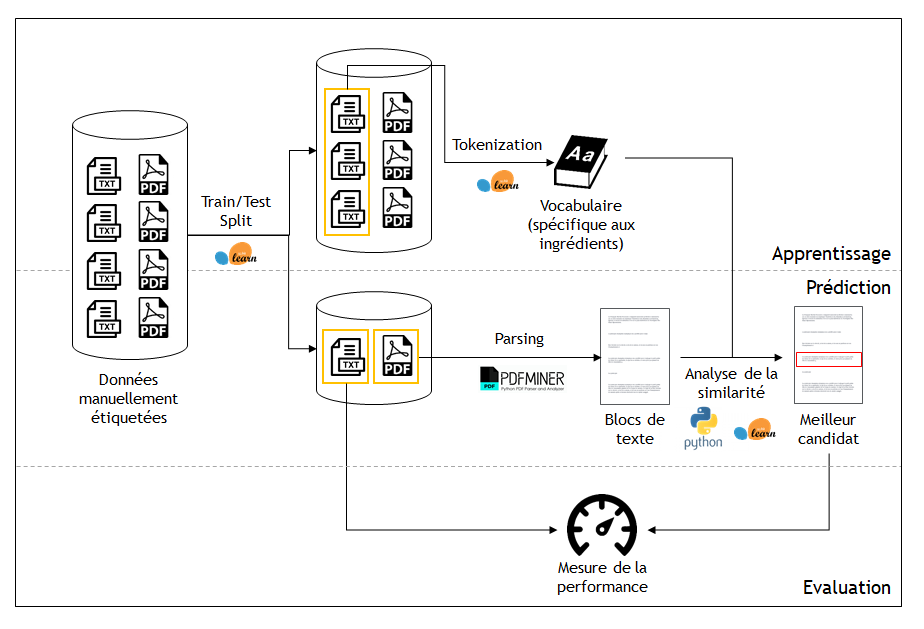
\includegraphics[width=0.9\linewidth]{img/measured_model.png}
        \end{center}
        \caption{Illustration de la méthodologie de mesure de la performance}
        \label{fig:measured_model}
    \end{figure}     

        \section{Accuracy}
        
        La métrique qui tombe le plus sous le sens est l'accuracy (on utilisera le terme anglais pour éviter les confusions avec la notion de \og precision \fg telle qu'elle est utilisée par exemple dans le f1-score).
        On mesure simplement la proportion de prédictions qui sont égales à la ground truth.
        La méthodologie utilisée est détaillée dans le notebook \og Mesure de la performance \fg présenté en annexe \mref{code:performance_measurement}.

            \subsection{Approche naïve}

                \subsubsection{Description de cette approche}

                L'approche \og naïve \fg consiste simplement à mesurer la proportion de textes prédits strictement égaux à la ground truth.
                Or, comme cela a été vu précédemment : 
                \begin{itemize}
                    \item les règles d'étiquetage manuel, détaillées à l'annexe \mref{annotation_rules}, montrent que des transformations sont parfois appliquées au contenu des listes d'ingrédients des pièces jointes avant d'établir la ground truth
                    \item les textes à comparer sont longs (jusqu'à quelques centaines de caractères), cf. \reftable{tbl:GT_prediction_sample}
                    \item la mise en forme, en particulier les retours à la ligne, ne sont pas positionnés aux mêmes endroits. Dans le parsing des documents pdf, lorsque le texte revient à la ligne après avoir atteint le bord de la page, l'outil positionne un retour à la ligne. Ce comportement n'a pas été reproduit dans l'établissement de la ground truth
                    \item le découpage en blocs de texte, de manière simple, produit des textes qui ne sont pas toujours le reflet du contenu spatialisé de ce document (cf. l'exemple donné à la section \mref{blocks_examples}, et la fiche technique associée en annexe \mref{ex:FT_meltrappeur})
                \end{itemize}
                On s'attend donc à avoir une \og accuracy naïve \fg faible.

                \subsubsection{Les résultats obtenus}

                Comme présenté dans notebook \og Analyse de la performance \fg (cf. annexe \mref{code:performance_measurement}), les résultats obtenus sont conformes à l'attendu.
                L'accuracy est très faible : 1\% (1 échantillon sur 100 produits) lorsqu'on la mesure sur l'échantillon de test après entraînement sur l'échantillon d'entraînement.
                Le seul produit pour lequel la liste d'ingrédients a été correctement identifiée porte les ingrédients suivants.
                \begin{quotation}
                    Sirop de glucose, sucre, eau, stabilisants (E440i, E440ii, E415), acidifiants (E330, E450i), conversateur (E202).
                \end{quotation}
                Si on effectue une cross-validation sur l'ensemble des données étiquetées, en appliquant un découpage en 10 folds, on obtient une accuracy moyenne de $1.80\% \pm 1.89\%$.

                \subsubsection{Nécessité d'améliorer cette métrique}
                On a vu que l'accuracy calculée de manière naïve porte un jugement sévère sur la performance du modèle.
                Par exemple, à la troisième ligne de la \reftable{tbl:GT_prediction_sample}, on voit bien que la liste d'ingrédients prédite est identique à la ground truth, si ce n'est qu les retours à la ligne ne sont pas positionnés exactement au même endroit.
                Comme on souhaite pouvoir ajuster le modèle, il est nécessaire d'avoir une métrique de mesure de la performance qui soit plus précise.

            \subsection{Avec du \og text-postprocessing \fg}
            \label{text_postprocessing}

                \subsubsection{Le principe}
                Afin de pallier ces problèmes de mise en forme de texte, on assouplit un peu les contraintes par rapport à l'égalité stricte.
                En effectuant un traitement de text processing, à la fois sur la ground truth et les résultats du modèle, on va comparer des textes un peu plus \og standardisés \fg.
                Les traitements effectués sont les suivants :
                \begin{itemize}
                    \item On passe le texte en minuscules
                    \item On retire la ponctuation
                    \item On remplace tous les \og whitespaces \fg (retours à la ligne, espaces multiples, tabulations, \dots) par des espaces simples
                    \item On retire les accents
                \end{itemize}
                L'ensemble de ces transformations sont faites en utilisant les fonctionnalités proposées par le CountVectorizer de la bibliothèque scikit-learn (cf. le notebook en annexe \mref{code:performance_measurement} et le module pimest inclus en annexe \mref{code:pimest}).

                \subsubsection{Les résultats}

                Si on évalue cette nouvelle accuracy avec le text processing, sur l'échantillon d'entraînement après entraînement sur l'échantillon d'entraînement, on obtient une accuracy de 14\% (14 listes d'ingrédients correctement prédites sur 100).
                Ces 14 listes d'ingrédients sont présentées à la \reftable{tbl:GT_postprocessed_corrects}.

               {\renewcommand{\arraystretch}{1.5}%
                \begin{table}
                    \begin{spacing}{1.0}
                    \begin{center}
                    {\scriptsize
                    \begin{tabular}{p{7cm}p{7cm}}
\toprule
                                                                                                                                                                                                                                                                                                                                   Liste d'ingrédients cible &                                                                                                                                                                                                                                                                                                                                        Liste d'ingrédients prédite \\ \hline
\midrule
                                                                                                                                                                                                                                                                          Gésier de dinde émincé 50\%, graisse de canard 47\%, sel, arômes naturels de poivre. &                                                                                                                                                                                                                                                                            Gésier de dinde émincé 50\%,  graisse de canard 47\%, sel, arômes naturels de poivre.  \newline   \\ \hline
 Edulcorants sorbitol, isomalt, sirop de maltitol, aspartame, mannitol, sel d'aspartame-acesulfame, acesulfame-k, sucralose; gomme base (contient de la lecithine de SOJA), aromes, epaississant gomme arabique, humectant glycerol, colorant E171, agent d'enrobage cire de carnauba, colorant E163, antioxygene BHA. Contient une source de PHENYLALANINE. &  Edulcorants sorbitol, isomalt, sirop de maltitol, aspartame, mannitol, sel d'aspartame-acesulfame, acesulfame-k, sucralose;  \newline gomme base  (contient de la lecithine de SOJA), aromes, epaississant gomme arabique, humectant glycerol, colorant E171,  \newline agent d'enrobage cire de carnauba, colorant E163, antioxygene BHA. Contient une source de PHENYLALANINE.  \\ \hline
                                                                                                                                                                                                        mini poivrons jaunes, eau, sucre, sel, affermissant chlorure de calcium : E509, acidifiant : acide citrique, vinaigre, antioxydant : vitamine C E330 &                                                                                                                                                                                                          mini poivrons jaunes, eau, sucre, sel, affermissant chlorure de  \newline calcium : E509, acidifiant : acide citrique, vinaigre, antioxydant :  \newline vitamine C E330  \\ \hline
                                                                    Farine de BLE, huile de colza non hydrogénée, OEUFS de poules élevées en plein air (21\%), sucre, stabilisant : glycérol, sirop de glucose-fructose, émulsifiant : mono- et diglycérides d'acides gras, poudres à lever : diphosphates et carbonates de sodium (BLE), fécule, sel, arôme. &                                                                         Farine de BLE, huile de colza non hydrogénée, OEUFS de poules élevées en plein air (21\%), sucre, stabilisant : glycérol, sirop de glucose-fructose, émulsifiant : mono- et diglycérides d'acides gras,  \newline poudres à lever : diphosphates et carbonates de sodium (BLE), fécule, sel, arôme. \\ \hline
                                                                                                                              Pommes de terre 59,5 \% - Céleris 40 \% - Amidon de maïs - Sirop de glucose de maïs - Huile de colza - Emulsifiants : E322, E471 - Stabilisant : E450i - Curcuma - Conservateur : E223 - Antioxydant : E304 - Acidifiant : E330. &                                                                                                                                   Pommes de terre 59,5 \% - Céleris 40 \% - Amidon de maïs - Sirop de glucose de maïs - Huile de colza - Emulsifiants : E322, E471 - Stabilisant : E450i  \newline - Curcuma - Conservateur : E223 - Antioxydant : E304 - Acidifiant : E330. \\ \hline
                                                                                                                                                                                                                                                                                                                                                      <rien> &                                                                                                                                                                                                                                                                                                                                                             <rien> \\ \hline
                                                      Amidon de maïs* - Lait écrémé* - Sel - Fécule de pomme de terre* - Tomate* - Oignon* - Arômes naturels - Poivres* 3 \% (poivre vert*, poivre blanc*, poivre noir*) - Huile de tournesol* - Extrait de levure* - Sucre caramélisé* - Ail* - Maltodextrine de maïs*. \newline * issus de l'agriculture biologique &                                                          Amidon de maïs* - Lait écrémé* - Sel - Fécule de pomme de terre* - Tomate* - Oignon* - Arômes naturels - Poivres* 3 \% (poivre vert*, poivre blanc*,  \newline poivre noir*) - Huile de tournesol* - Extrait de levure* - Sucre caramélisé* - Ail* - Maltodextrine de maïs*.  \newline * issus de l’agriculture biologique \\ \hline
                                                                                                                                                             Farine de FROMENT, poudre de LACTOSERUM, sucre, poudre d'OEUF entier, poudres à lever: (E450, E500), matière grasse LAITIERE, sel. \newline Peut contenir des traces de : soja, fruits à coques, lupin. &                                                                                                                                                                  Farine de FROMENT, poudre de LACTOSERUM, sucre, poudre d'OEUF entier, poudres à lever: (E450,  \newline E500), matière grasse LAITIERE, sel. \newline Peut contenir des traces de : soja, fruits à coques, lupin. \\ \hline
                                                                                                                                                        Eau, maltodextrine, sel, arômes, sucre, arôme naturel de citronnelle, amidon modifié, ail en poudre, épices (combava, curcuma), extraits d'épices (gingembre, poivre), stabilisant (gomme xanthane). &                                                                                                                                                          Eau, maltodextrine, sel, arômes, sucre, arôme naturel de citronnelle, amidon modifié, ail en poudre, épices (combava, curcuma), extraits  \newline d'épices (gingembre, poivre), stabilisant (gomme xanthane).    \\ \hline
                                                                                        OEUFS, farine de BLE, sucre, amidon de BLE, stabilisants: sorbitols- glycérol, cacao maigre en poudre (3,5\%), émulsifiants: E472b - E477, poudres à lever: E450 - E500, sirop de glucose, LAIT écrémé en poudre, sel, conservateur: E202, épaississant: E410, arôme. &                                                                                             OEUFS, farine de BLE, sucre, amidon de BLE, stabilisants: sorbitols- glycérol, cacao maigre en poudre (3,5\%), émulsifiants: E472b - E477, poudres à lever: E450 - E500, sirop de glucose, LAIT  \newline écrémé en poudre, sel, conservateur: E202, épaississant: E410, arôme. \\ \hline
                                                                                                                                                                                                                                           Sirop de glucose, sucre, eau, stabilisants (E440i, E440ii, E415), acidifiants (E330, E450i), conversateur (E202). &                                                                                                                                                                                                                                                  Sirop de glucose, sucre, eau, stabilisants (E440i, E440ii, E415), acidifiants (E330, E450i), conversateur (E202). \\ \hline
                                                                                                                                                                                                                                                                                 Flageolets verts. Jus : eau, sel, affermissant : chlorure de calcium (E509) &                                                                                                                                                                                                                                                                                       Flageolets verts. Jus : eau, sel, affermissant : chlorure de calcium (E509)  \\ \hline
                                                                                                                                                                                                                                                      Carottes, eau, sucre, sel, vinaigre d'alcool, acidifiant : acide lactique. Présence fortuite de CELERI &                                                                                                                                                                                                                                                             Carottes, eau, sucre, sel, vinaigre d’alcool, acidifiant : acide lactique. Présence fortuite de CELERI \\ \hline
                                                                                                                                               Légumes 43,2 \% (pomme de terre, oignon, carotte, tomate, poireau) - Amidon modifié de pomme de terre - Extrait de levure - Sirop de glucose de maïs - Huile de colza - Sucre - Arôme naturel - Ail - Curcuma. &                                                                                                                                                    Légumes 43,2 \% (pomme de terre, oignon, carotte, tomate, poireau) - Amidon modifié de pomme de terre - Extrait de levure - Sirop de glucose de maïs -  \newline Huile de colza - Sucre - Arôme naturel - Ail - Curcuma. \\ \hline
\bottomrule
\end{tabular}

                    }
                    \caption{Prédictions identifiées comme correctes après postprocessing}
                    \label{tbl:GT_postprocessed_corrects}
                    \end{center}
                    \end{spacing}
                \end{table}
                }

                De la même manière que précédemment, si on fait une cross-validation sur l'ensemble des données manuellement étiquetées, on obtient une accuracy de $16.60\% \pm 3.35\%$.

                \subsubsection{Les limites de cette métrique}

                Cette métrique est déjà plus intéressante que l'approche naïve, mais elle a quand même un défaut majeur : elle a une vision encore trop binaire des résultats.
                En effet, que le texte soit identique à un préfixe près (cf. la quatrième ligne de la \reftable{tbl:GT_prediction_sample}), ou qu'il n'ait rien à voir (d'autres exemples sont présents dans cette même table), elle considèrera la prédiction comme erronée.
                Or, il est important d'identifier les cas où le modèle s'est complètement trompé par rapport à ceux où il a quand même identifié le bon bloc contenant les ingrédients.

        \section{Fonctions de \og similarité \fg spécifiques}

        On peut définir des fonctions de similarité, qui permettent d'être plus fin qu'une simple évaluation binaire du résultat du modèle.
        Cela permet de prendre plus finement en compte les cas où le modèle a identifié un bloc très similaire à la ground truth.
        On va pour cela s'appuyer sur diverses métriques permettant de mesurer l'écart entre des chaînes de caractères.
        \`{A} chaque fois, on définira une fonction de scoring qui sera une similarité.
        De plus, elles seront normées pour prendre leurs valeurs entre 0 (chaînes de caractères totalement différentes) et 1 (chaînes identiques), ce qui permettra d'exprimer ces métriques en pourcentage.
        Ces similarités seront calculées après application du text-postprocessing, comme décrit à la section \mref{text_postprocessing}.
        L'ensemble de ces similarités seront calculées sur les caractères.

            \subsection{Similarité basée sur la distance de Levenshtein}

            La distance de Levenshtein~\cite{levenshtein_wiki}  entre deux chaînes de caractères est la distance d'édition pour passer de l'une à l'autre en prenant en compte les transformations suivantes :
            \begin{itemize}
                \item insertion d'un caractère 
                \item suppression d'un caractère
                \item substitution d'un caractère par un autre
            \end{itemize}
            Cette distance possède les caractéristiques suivantes : 
            \begin{itemize}
                \item elle peut se calculer entre deux chaînes de longueur différentees
                \item elle a pour minimum 0 (si et seulement si les deux chaines sont identiques)
                \item a pour majorant la longueur de la plus longue des deux châines
            \end{itemize}
            Pour construire une fonction de similarité telle que présentée en introduction de cette section, on appliquera la transformation suivante : 
            \[sim_{lev}(s_{1}, s_{2}) = 1 - \frac{dist_{lev}(s_{1}, s_{2})}{max(len(s_{1}), len(s_{2}))}\]
            en notant $dist_{lev}$ la distance de Levenshtein, $len(s)$ la longueur de la chaîne $s$, et $s_{1}$ et $s_{2}$ les chaînes de caractères à comparer.
            Par exemple, la distance entre les chaînes \og rateaux \fg et \og chameau \fg vaut 4 :
            \begin{itemize}
                \item substitution du \og r \fg par un \og c \fg
                \item insertion du \og h \fg
                \item substitution du \og t \fg par un \og m \fg
                \item suppression du \og x \fg
            \end{itemize}

            \subsection{Similarité basée sur la distance de Damerau-Levenshtein}

            La distance de Damerau-Levenshtein~\cite{damerau_levenshtein_wiki} est une variante de la distance de Levenshtein.
            Elle calcule également une distance d'édition, mais en ajoutant une transformation possible : l'interversion de deux caractères successifs.
            Les transformations possibles pour cette transformation sont :
            \begin{itemize}
                \item insertion d'un caractère 
                \item suppression d'un caractère
                \item substitution d'un caractère par un autre
                \item interversion de deux caractères successifs
            \end{itemize}
            Ses caractéristiqes sont les mêmes que la distance de Levenshtein (minimum, maximum) ; et elle est toujours inférieure ou égale à la distance de Levenshtein.
            On convertit cette distance en similarité de la même manière que la distance de Levenshtein.

            \subsection{Similarité de Jaro}
            
            La similarité de Jaro~\cite{jaro_wiki} est une fonction permettant de mesurer une similarité entre 0 (chaînes complètement différentes) et 1 (chaînes parfaitement identiques).
            L'heuristique derrière cette similarité est de considérer qu'entre deux chaînes, un caractère est \og correspondant \fg (\og matching \fg) s'il est déplacé de moins de la moitié de la longueur de la plus longue des deux chaînes.
            Ensuite, la similarité est fonction croissante du nombre de caractères \og correspondants \fg et décroissante du nombre de caractères \og correspondants \fg mais mal placés.
            Sur des chaînes longues de quelques dizaines de caractères, la quasi-totalité des caractères seront \og correspondants \fg.
            Elle est en général plutôt adaptée à des comparaison de chaînes courtes telles que des noms propres ou des mots de passe.

            \subsection{Similarité de Jaro-Wrinkler}
            
            La similarité de Jaro-Winkler~\cite{jaro_winkler_wiki} est une variante de la similarité de Jaro.
            Elle possède la même heuristique que la distance de Jaro, avec en plus comme caractéristique de donner un poids plus important aux 4 caractères formant le début de la chaîne de caractères.
            Cette métrique est encore moins adaptée au cas d'usage que la précédente.

            \subsection{\'{E}valuation de ces similarités sur la ground truth}

            Les résultats de l'évaluation de chacune de ces similarités sont présentés à la \reftable{tbl:similarities_result}.
            \begin{table}[htbp]
                \begin{center}
                \begin{tabular}{lcc}
\toprule
{} & train/test set & cross validation \\
\midrule
\textbf{Levenshtein        } &         48.86\% &  49.79\% +/-3.73\% \\
\textbf{Damerau-Levenshtein} &         48.86\% &  49.80\% +/-3.72\% \\
\textbf{Jaro               } &         63.56\% &  62.78\% +/-3.28\% \\
\textbf{Jaro-Winkler       } &         65.67\% &  64.40\% +/-3.50\% \\
\bottomrule
\end{tabular}

                \caption{\'{E}valuation du modèle en utilisant les métriques de similarité}
                \label{tbl:similarities_result}
                \end{center}
            \end{table}
            On constate que :
            \begin{itemize}
                \item les similarités de Levenshtein et Damerau-Levenshtein donnent des résultats identiques
                \item les similarités de Jaro et de Jaro-Winkler donnent des évaluations très généreuses de la performance du modèle, comme on pouvait s'y attendre sur la base de textes longs
            \end{itemize}

            \subsection{Décision sur la métrique à utiliser et illustration}
            
            Les similarités de Jaro et Jaro-Winkler sont abandonnées car non pertinentes pour notre cas d'usage, qui se base sur des textes de plusieurs dizaines de caractères.
            Les similarités de Levenshtein et Damerau-Levenshtein donnant des résultats identiques, on choisit la distance de Levenshtein car son implémentation en C (bibliothèque python-Levenshtein) semble plus performante que celle en C++ de la bibliothèque Jellyfish.

            Des exemples du début, du milieu et du bas du classement en termes de similarité de Levenshtein sur le jeu de test, après entraînement sur le jeu d'entraînement, sont présentés à la \reftable{tbl:similarity_illustration}.
            \begin{table}[htbp]
                \begin{spacing}{1.0}
                \begin{center}
                {\tiny
                \begin{tabular}{p{5cm}p{5cm}cccc}
\toprule
                                                                                                                                                                                                                                                              Listes d'ingrédients cibles &                                                                                                                                                                                                                                                                                             Listes d'ingrédients prédites &     Lev & Dam-Lev &    Jaro & Jaro-Win \\ \hline
\midrule
                                                                                                                                                                                                       Gésier de dinde émincé 50\%, graisse de canard 47\%, sel, arômes naturels de poivre. &                                                                                                                                                                                                                                   Gésier de dinde émincé 50\%,  graisse de canard 47\%, sel, arômes naturels de poivre.  \newline   & 100.00\% & 100.00\% & 100.00\% &  100.00\% \\ \hline
                                                                                                                                     mini poivrons jaunes, eau, sucre, sel, affermissant chlorure de calcium : E509, acidifiant : acide citrique, vinaigre, antioxydant : vitamine C E330 &                                                                                                                                                                 mini poivrons jaunes, eau, sucre, sel, affermissant chlorure de  \newline calcium : E509, acidifiant : acide citrique, vinaigre, antioxydant :  \newline vitamine C E330  & 100.00\% & 100.00\% & 100.00\% &  100.00\% \\ \hline
 Farine de BLE, huile de colza non hydrogénée, OEUFS de poules élevées en plein air (21\%), sucre, stabilisant : glycérol, sirop de glucose-fructose, émulsifiant : mono- et diglycérides d'acides gras, poudres à lever : diphosphates et carbonates de sodium (BLE), fécule, sel, arôme. &                                Farine de BLE, huile de colza non hydrogénée, OEUFS de poules élevées en plein air (21\%), sucre, stabilisant : glycérol, sirop de glucose-fructose, émulsifiant : mono- et diglycérides d'acides gras,  \newline poudres à lever : diphosphates et carbonates de sodium (BLE), fécule, sel, arôme. & 100.00\% & 100.00\% & 100.00\% &  100.00\% \\ \hline
                                                                                                                                                                                                                                                               Pommes de terre, eau, sel. &                                                                                                                                                                                                                                  Anhydride sulfureux et sulfites en  \newline concentrations de plus de 10 mg/kg  \newline exprimé en SO2 &  15.48\% &  15.48\% &  48.29\% &   48.29\% \\ \hline
%                                                                                                                                                                                                                                           Débris de truffes d'hiver, jus de truffes, sel &                                               \newline Origine Truffes et Sel          :           France et/ou Espagne  \newline   \newline Traçabilité                            :          Chaque lot est enregistré et identifié.  \newline   \newline Caractéristiques organoleptiques : Débris de couleur hétérogène (marron à noir)  sans colorant, dans  &  14.97\% &  14.97\% &  47.87\% &   47.87\% \\ \hline
                                                                                                                                                                                                                                                                     AMANDES décortiquées &                                                                                                       Valeur énergétique :  \newline      Matières grasses :   \newline           dont ac gras saturés :  \newline      Glucides :  \newline           dont sucres :   \newline      Fibres alimentaires :        Dietary fibre  \newline      Protéines :  \newline      Sel :   &  12.80\% &  12.80\% &  46.93\% &   46.93\% \\ \hline
                                                                                                                                                                                                                                              Poire 99,9\%, antioxydant: acide ascorbique. &  Ce produit est une purée de fruits obtenue à partir des parties comestibles des fruits (après broyage et sans  \newline concentration notable). \newline Ce produit est sans sucres ajoutés: il contient uniquement les sucres naturellement présents dans les fruits. \newline La purée présente une texture homogène et légèrement granuleuse. &   9.67\% &   9.67\% &  43.73\% &   43.73\% \\ \hline
                                                                                                                                                                                                                                                                 100\% haricots blancs bio &                              Les légumes secs sont mis en avant par tous les nutritionnistes pour leurs apports en protéines et fibres. Ils s’inscrivent parfaitement  \newline dans le PNNS.  \newline Les légumes secs bio bénéficient également d’une agriculture résonnée et donne des garanties en termes de développement durable.  &   6.62\% &   6.62\% &  35.47\% &   35.47\% \\ \hline
                                                                                                                                                                                                                                                                                   Persil &                                                                                                                                                                         Céréales contenant du gluten (à savoir blé, seigle, orge, avoine, épeautre, Kamut ou leurs souches hybrides) \newline et Produits à base de ces Céréales. &   4.55\% &   4.55\% &  50.76\% &   50.76\% \\ \hline
\bottomrule
\end{tabular}

                }
                \caption{Illustration de l'évaluation du modèle à l'aide des métriques de similarité}
                \label{tbl:similarity_illustration}
                \end{center}
                \end{spacing}
            \end{table}

        \subsection{Performance en fonction de la longueur de la liste d'ingrédients}

        \`{A} la section \mref{prediction_gt_illustration}, on avait mentionné le fait que le modèle semblait moins performant lorsque la liste d'ingrédients cible était courte.
        Maintenant que nous avons une fonctionnalité de mesure de la performance, il est possible de confirmer ou d'infirmer ce point.
        La représentation de ce lien est présentée en \reffig{fig:perf_vs_length}.
        Il y a bien une corrélation positive entre longueur de la liste d'ingrédients et performance du modèle ($r^{2} \approx 0.340$, après retrait des outliers).
        Le mode de production de ce graphe est présenté à la fin du notebook \og Mesure de la performance \fg inclus en annexe \mref{code:performance_measurement}.
        \begin{figure}[htbp]
            \begin{center}
            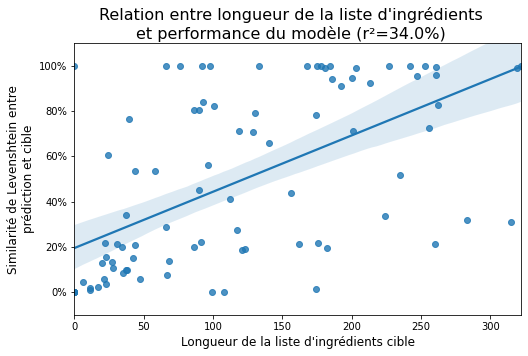
\includegraphics[width=0.7\linewidth]{img/perf_vs_length.png}
            \end{center}
            \caption{Performance du modèle en fonction de la longueur des listes d'ingrédients}
            \label{fig:perf_vs_length}
        \end{figure}

    \chapter{Ajustement des paramètres}
    \label{model_tuning}

        \section{Description des paramètres ajustables}

        Les paramètres ajustables sur le modèle présenté ci-dessus sont multiples (text-preprocessing, découpage des textes en blocs, calcul de similarité, \dots).
        Maintenant qu'un pipeline équipé d'une fonctionnalité de mesure de la performance est disponible, on va pouvoir faire varier les paramètres et évaluer l'impact sur la performance du modèle.

        \subsection{Text-preprocessing}

        L'étape de text-preprocessing vise à nettoyer et standardiser le contenu des textes.
        Elle est appliquée aux textes avant entraînement et avant prédiction.
        Il est nécessaire de bien appliquer les mêmes règles à ces deux étapes.
        Parmi les fonctionnalités classiques de texte préprocessing, on va procéder de la manière suivante : 

        \emph{Mise en minuscule} : 
        On appliquera systèmatiquement la mise en minuscule. 
        La casse est plutôt un facteur qui va pénaliser l'interprétation du texte, en contribuant à la création artificielle de mots synonymes.

        \emph{Retrait des accents} : 
        L'impact du retrait des accents sera mesuré sur la performance du modèle.
        En effet, même s'il peut amener à la création d'homonymes, sur des textes en français inclus dans des pdf et issus de multiples sources cette fonctionnalité peut avoir une influence positive.

        \emph{Gestion des stopwords} : 
        On vérifiera l'impact de retirer les stopwords (mots fréquents peu porteurs de sens) de l'ensemble des textes (listes d'ingrédients cible, contenu des documents) avant entraînement ou prédiction.
        On se basera sur une liste déterminée à partir des mots les plus fréquents dans le corpus des documents, qui ne portent pas de signification.
        Il est pressenti que ces stopwords risquent d'avoir un impact important sur le résultat de l'algorithme, en ajoutant dans l'ensemble des blocs candidats un grand nombre de mots étant considérés comme des ingrédients.

        \subsection{Découpage du texte des documents en blocs}
        \label{splitting_functions}

        On peut envisager d'autres méthodes de découpage des textes complets des documents en blocs candidats.
        Il avait été vu lors du prototypage que cette fonction pouvait influer fortement sur la qualité du résultat (il est inutile de chercher une bonne solution pour trouver le bon candidat si on détermine mal la liste de candidats).
        On éprouvera les techniques suivantes : 
        \begin{itemize}
            \item comme en prototypage, en coupant dès que deux retours à la lignes successifs sont identifiés
            \item à chaque retour à la ligne
            \item via une expression régulière, on coupera dès qu'on trouve un ensemble de whitespaces (espaces, retour à la ligne, tabulation, \dots) contenant au moins 2 retours à la ligne
        \end{itemize}
        
        \subsection{Vectorisation des textes}
        \label{vectorisation}

        \emph{Bag Of Words} : 
        Les textes seront représentées sous forme de vecteurs via l'approche \og Bag Of Words \fg.
        On évaluera les méthodes suivantes pour la transformation des textes en vecteurs :
        \begin{itemize}
            \item de manière binaire : la coordonnée est à 1 si le mot est présent au moins une fois dans le texte, 0 sinon
            \item en term-frequency (tf) : la coordonnée correspond à la fréquence d'apparition du mot dans le texte
            \item en tf-idf, l'inverse document frequency pouvant être calculée en référence au corpus du contenu des documents
            \item via une fonction de score absolu, tel que décrit dans la partie sur l'analyse des données, à la section \mref{word_scores}
            \item via une fonction de score relatif (décrit dans la même section)
        \end{itemize}
        
        \emph{n-grams} : 
        On testera également la possibilité de prendre en compte des n-grams de mots (mots successifs) et les résultats que cela amène (à la fois dans l'entraînement et dans la prédiction).

        \emph{Embeddings des mots} : 
        Enfin, on procédera aux calculs d'embeddings de mots, en appliquant les méthodes suivantes :
        \begin{itemize}
            \item truncated SVD~\cite{LSA_wiki} : on approxime la matrice des textes vectorisés en calculant ses valeurs singulières et en n'en gardant que les 100 plus importantes (valeur choisie arbitrairement). Les embeddings des mots sont récupérable directements depuis le transformateur TruncatedSVD mis à disposition dans la bibliothèque scikit-learn.
            \item Word2Vec~\cite{word2vec_wiki} : cette méthode de calcul des embeddings se base sur l'entrainement d'un réseau de neurones pour la prédiction d'un mot à partir des autres mots de son contexte (Continuous Bag Of Words, CBOW), ou de prédire le contexte à partir d'un mot (skip-gram). Les embeddings sont les poids de la couche intermédiaire du réseau de neurones après entraînement. On utilisera l'algorithme CBOW, avec un nombre de features de 100.
        \end{itemize}
        Cette manière de représenter les textes et les mots se traduit par une \emph{réduction de la dimensionalité}, qui passe du nombre de mots dans le vocabulaire (plus de 10 000 dans notre cas) au nombre de features conservées (on en gardera 100).

        \subsection{Calcul de similarité}

            \subsubsection{Similarité cosinus}
            \label{similarite_cosinus}

            Cette méthode nécessite de représenter le vocabulaire des ingrédients sous la forme d'un vecteur, en faisant la moyenne des vecteurs de textes obtenus lors de la vectorisation des listes d'ingrédients.
            On calcule le cosinus de l'angle entre le vecteur du vocabulaire et celui du candidat.
            Plus ce cosinus est élevé, plus la similarité est importante.
            Cette similarité n'a pas de paramètre, une fois que les vecteurs ont été calculés.
            Il est possible d'appliquer ce calcul de similarité y compris après application d'un embedding des vecteurs de texte (ex: Word2Vec, tSVD, \dots).
            Une illustration de la similarité cosinus est proposée à la \reffig{fig:similarite_cosinus}.
            Enfin, ce mode de calcul de la similarité permet d'ajuster la direction du vecteur cible en fonction de divers critères (fonctions de scoring spécifiques, cf. section \mref{vectorisation} sur la vectorisation des textes).
            La similarité cosinus est toujours comprise entre 0 (vecteurs orthogonaux) et 1 (vecteurs colinéaires), sauf dans le cas où on applique des coefficients négatifs à certains mots (cas de la fonction de scoring relatif, où des poids sont négatifs).

            \subsubsection{Par projection}
            \label{similarite_projection}

            Cette méthode nécessite uniquement de projeter le candidat sur le sous-espace généré par les mots du vocabulaire des ingrédients.
            On fait ensuite le rapport entre la norme du vecteur initial, à celle de sa projection. 
            On peut envisager cette similarité un peu comme un calcul de l'angle entre le vecteur candidat et le sous-espace cible.
            Attention, si on utilise la même norme pour mesurer le vecteur initial et sa projection, on choisira toujours les candidats dont aucun mot n'est hors du vocabulaire (cf. l'illustration présentée à la \reffig{fig:similarite_projection}).
            Une manière de s'affranchir de ceci est choisir pour mesurer le vecteur initial une norme $L_{p}$ et pour sa projection une norme $L_{q}$ avec $p > q$.
            En effet, un résultat d'algèbre linéaire~\cite{lpnorms} montre que :
            \[\forall x \in \mathbb{R}^{n}, \; p > q \Rightarrow \lVert x \rVert_{p} \leqslant \lVert x \rVert_{q}\]
            Pour rappel, la norme $L_{p}$ d'un vecteur $x$ est définie par : 
            \[\lVert x \rVert_{p} = \left( \sum_{i} |x_{i}|^{p} \right)^{1/p} \]
            où les $x_{i}$ sont les coordonnées de $x$.
            Ce calcul de similarité ne peut se faire que dans l'espace initial, où les vecteurs représentant les textes peuvent être projetés sur un espace généré par des mots.
            Si une réduction de la dimensionalité a eu lieu, par exemple via le calcul d'embeddings, il n'est pas possible de déterminer un sous-espace généré par les mots du vocabulaire des ingrédients.
            De plus, contrairement au calcul de similarité cosinus, il n'est pas possible de pondérer les différents mots du vocabulaire des ingrédients (via un calcul de score spécifique, un tf-idf, \dots).
            Ce mode de calcul est paramétrique, c'est à dire qu'il faut définir la norme de l'espace de départ et la norme dans le sous-espace de projection.
            Contrairement à la similarité cosinus, la similarité projection peut être supérieure à 1.

            Le mode de calcul retenu dans les prototypes décrits précédemment (chapitre \mref{prototypes}) est un calcul de similarité par projection utilisant les normes $L_{2}$ sur l'espace initial et $L_{1}$ sur le sous-espace de projection.
            La formule de calcul était : 
            \[\frac{\text{Nombre de mots du candidat qui sont des ingrédients}}{\text{Norme euclidienne du vecteur du candidat}} = \frac{\lVert\text{Vecteur projeté}\rVert_{1}}{\lVert\text{Vecteur initial}\rVert_{2}}\]
            où le vecteur initial est la matrice des textes avec les comptes de mots.

            \subsubsection{Illustration de ces calculs de similarité}

            On illustre ces deux manières de mesurer la similarité en prenant l'exemple suivant.
            Le vocabulaire des ingrédients est constitué des mots \og eau \fg et \og sucre \fg, et le mot \og eau \fg est 2 fois plus représenté que le mot \og sucre \fg.
            Les textes candidats sont \og sucre eau sucre \fg et \og commercial commercial sucre \fg.
            Ces deux exemples sont présentés en \reffig{fig:similarite_cosinus} et \reffig{fig:similarite_projection}.
            Sur ces figures, la similarité correspond aux angles matérialisés en vert.
            Si on récapitule les valeurs respectives des similarités, on obtient les résultats présentés à la \reftable{tbl:similarites_exemples}
            
            \begin{figure}[htbp]
                \begin{center}
                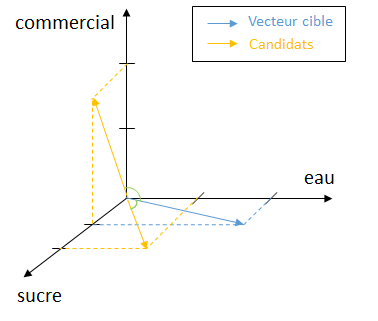
\includegraphics[width=0.5\linewidth]{img/similarite_cosinus.png}
                \end{center}
                \caption{Illustration de la similarité cosinus}
                \label{fig:similarite_cosinus}
            \end{figure}     

            \begin{figure}[htbp]
                \begin{center}
                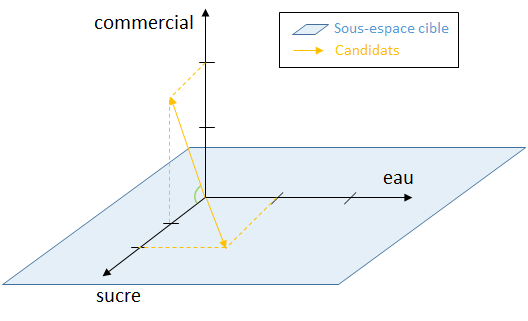
\includegraphics[width=0.6\linewidth]{img/similarite_projection.png}
                \end{center}
                \caption{Illustration de la similarité projection}
                \label{fig:similarite_projection}
            \end{figure}     

            \begin{table}[hbtp]
            \begin{center}
            \begin{small}
            \begin{tabular}{lcccc}
                \toprule
                \textbf{Candidats} &  \textbf{Cosinus} &  \textbf{Projection $L_{1}/L_{1}$} & \textbf{Projection $L_{2}/L_{1}$} & \textbf{Projection $L_{3}/L_{1}$}\\
                \midrule
                \textbf{sucre eau sucre} &  0,8 & 1, & 1,34 & 1,44 \\
                \textbf{commercial commercial sucre} & 0,2 & 0,33 & 0,45 & 0,48 \\
                \bottomrule
            \end{tabular}
            \end{small}
            \caption{Exemples de calculs de similarité}
            \label{tbl:similarites_exemples}
            \end{center}
            \end{table}

    \section{Ajustements et résultats}
            
    On peut, dans l'optique d'améliorer la performance du modèle, ajuster certains paramètres et d'évaluer l'impact via une grid search.
    Pour l'ensemble des ajustements, on travaillera uniquement sur le set d'entrainement (400 échantillons) afin de se prémunir des effets de data leaking (qui amènerait à surestimer la performance lors de l'évaluation finale).
    On travaillera avec 8 folds de cross-validation, afin de rester sur des ordres de grandeurs comparables à ce qui avait été fait lors de l'évaluation du second prototype (10 folds sur 500 échantillons).
    Enfin, on effectuera une évaluation finale sur le set de test, après entraînement du modèle avec les meilleures performances sur le set d'entraînement.
    La sélection des meilleurs paramètres se fera sur la base de la similarité de Levenshtein (cf. chapitre \mref{performance}), mais on illustrera également la performance du modèle retenu via l'accuracy avec text-postprocessing.
    L'ensemble des résultats présentés à cette section sont issus du notebook \og Tuning du modèle \fg présenté en annexe \mref{code:model_tuning}.

        \subsection{Ajustement du text-preprocessing}

            Les résulats de la grid search sur le text-preprocessing sont présentés à la \reffig{fig:tuning_prepro}.
            Dans l'ensemble des représentations de ce chapitre, chaque point du swarmplot représente une cross validation de l'ensemble du set de test.
            Les folds individuels ne sont pas représentés, l'écart type pour un jeu de paramètres donné n'est donc pas représenté (le détail est présenté dans le notebook mentionné précédemment).
            Dans ce premier run, les paramètres explorés sont : 
            \begin{description}
                \item[gestion des accents :] conservation ou retrait des accents sur les textes
                \item[gestion des stopwords :] conservation ou retrait des stopwords ('pas', 'le', 'en', 'pour', 'ou', 'ce', 'de', 'dans', 'du', 'and', 'un', 'sur', 'et', 'of', 'est', 'par', 'la', 'les', 'dont', 'au', 'des', 'que') des textes
                \item[constitution des ngrams :] seulement les monogrammes, puis monogrammes et bigrammes, puis monogrammes et bigrammes et trigrammes
                \item[découpage des textes en blocs :] comparatif des trois fonction présentées précédemment à la section \mref{splitting_functions}
                \item[fonctions de similarité :] identification du meilleur candidat par similarité cosinus, ou par projection $L_{2}/L_{1}$
            \end{description}
            soit un total de 72 jeux de paramètres testés.
            Il apparaît que :
            \begin{itemize}
                \item le retrait des stopwords a un impact fortement positif sur la performance de l'algorithme
                \item le retrait des accents a un impact positif mais relativement marginal
                \item l'écart-type sur la performance (similarité de Levenshtein) est très élevé au sein d'un jeu de paramètre testé : il se situe systématiquement aux alentours de 5-6\% pour une valeur moyenne autour de 50\%
            \end{itemize}

            \begin{figure}[htbp]
                \begin{center}
                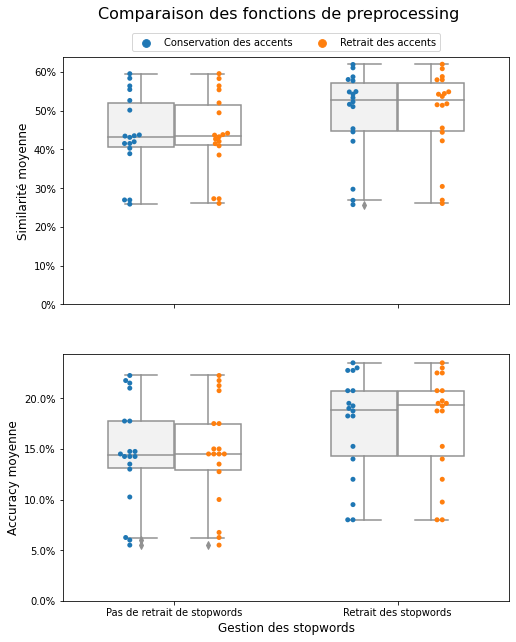
\includegraphics[width=0.9\linewidth]{img/tuning_prepro.png}
                \end{center}
                \caption{Résultats du tuning du preprocessing}
                \label{fig:tuning_prepro}
            \end{figure}     

            \subsection{Tuning du découpage du texte des documents}

            On se sert des résultats de la grid search présentée précédemment.
            Les résultats sont présentés à la \reffig{fig:tuning_split}.
            On en déduit que la fonction qui présente les meilleurs résultats est la troisième fonction (via une expression régulière avec 2 retours à la ligne).
            L'écart n'est pas énorme avec la fonction 1 (1 à 2\% sur l'accuracy moyenne), mais il est présent de manière consistante.

            \begin{figure}[htbp]
                \begin{center}
                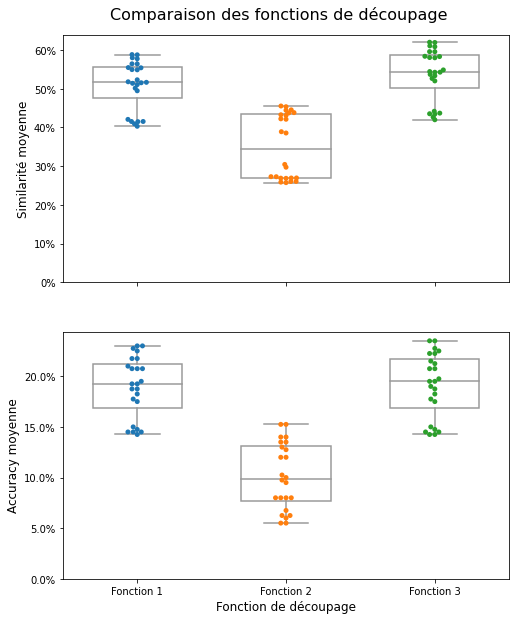
\includegraphics[width=0.9\linewidth]{img/tuning_split.png}
                \end{center}
                \caption{Résultats du tuning du découpage des textes des documents}
                \label{fig:tuning_split}
            \end{figure}

            \subsection{Comparatif des fonctions de similarité}

            Dans une seconde grid search, on va comparer les similarité cosinus et projection, en faisant varier les paramètres de la similarité projection (normes de l'espace complet et du sous-espace de projection).
            Les résultats sont présentés à la \reffig{fig:tuning_similarite}.
            Ils sont issus d'une grid search lors de laquelle on a fixé : 
            \begin{itemize}
                \item la tokenisation avec des monogrammes et des bigrammes
                \item le retrait des accents
                \item le retrait des stopwords
                \item la fonction de découpage en blocs numéro 3 (avec l'expression régulière)
            \end{itemize}
            et on a fait varier : 
            \begin{itemize}
                \item les fonctions de similarité, cosinus ou projection
                \item les normes utilisées, pour les fonctions de projection
                \item la construction de la matrice des textes entre les comptes de mots, ou l'identification uniquement de la présence / absence d'un terme (\og binary Bag Of Word \fg)
            \end{itemize}
            Dans la représentation qui en a été faite, on a regroupé ensemble les similarité projection en fonction de l'écart de valeur entre les normes dans l'espace initial et le sous-espace de projection (ex : pour la similarité projection $L_{3}/L_{1}$ cet écart vaut 2);
            En peut en tirer des conclusions intéressantes : 
            \begin{itemize}
                \item les écarts-types au sein d'une cross-validation sont toujours importants (5-6\% environ, sur la similarité de Levenshtein)
                \item la similarité par projection surperforme nettement la similarité cosinus
                \item comme on pouvait s'y attendre, les performances sont catastrophiques si on applique pour la similarité projection la même norme dans l'espace de départ et le sous-espace de projection (on choisira toujours un texte qui n'a aucun mot hors du vocabulaire des ingrédients, peu importe sa longueur)
                \item des tendances régulières se dessinent parmi les groupes avec un delta constant, bien visibles sur l'indicateur de performance en similarité : 
                \begin{itemize}
                    \item les performances semblent suivre deux tendances polynomiales avec des coefficient d'ordre maximal négatif, différentes selon que la tokenisation est binaire ou non
                    \item la tokenisation binaire est systématiquement meilleure que la tokenisation par comptes
                    \item on atteint un maximum de performance aux alentours des projections $L_{4}/L_{3}$, $L_{6}/L_{4}$, $L_{8}/L_{5}$
                \end{itemize}
            \end{itemize}

            \begin{figure}[htbp]
                \begin{center}
                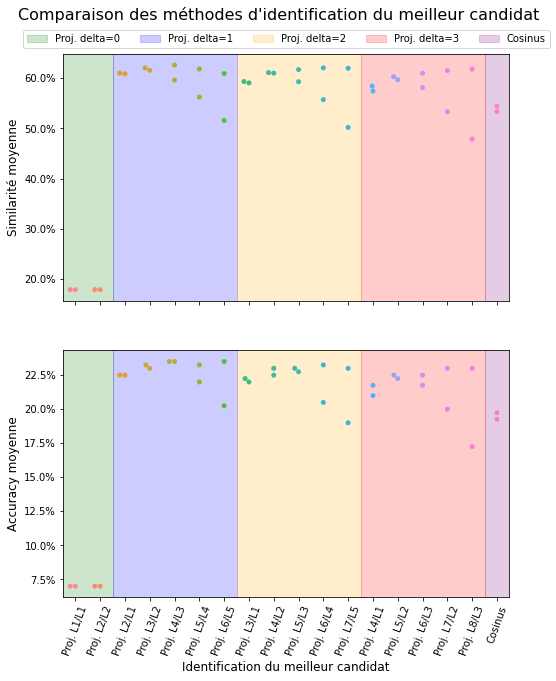
\includegraphics[width=0.9\linewidth]{img/tuning_similarite.png}
                \end{center}
                \caption{Résultats du tuning des fonctions de similarité}
                \label{fig:tuning_similarite}
            \end{figure}

            \subsection{Comparaison des méthodes de vectorisation}

            \subsubsection{Inverse document frequency}

            On peut apprécier l'impact de la prise en compte de l'inverse document frequency lors de la vectorisation, sur la performance du modèle.
            Cette inverse document frequency se calcule par rapport à la présence des termes dans le corpus des textes des documents.
            Les résultats sont présentés à la \reffig{fig:tuning_idf}, sur la base d'une grid search faisant varier : 
            \begin{itemize}
                \item le type de similarité : cosinus ou projection $L_{4}/L_{3}$
                \item l'utilisation ou non de l'inverse document frequency
                \item la prise en compte de ngrams, avec des ngrams de longueur de 1 à 5
            \end{itemize}
            L'impact est très différent selon qu'on identifie le meilleur candidat via le cosinus, plutôt que via la projection.
            La qualité des prédictions s'améliore en utilisant l'inverse document frequency couplée à la similarité cosinus, mais est très fortement dégradée dans le cas de la projection.

            \begin{figure}[htbp]
                \begin{center}
                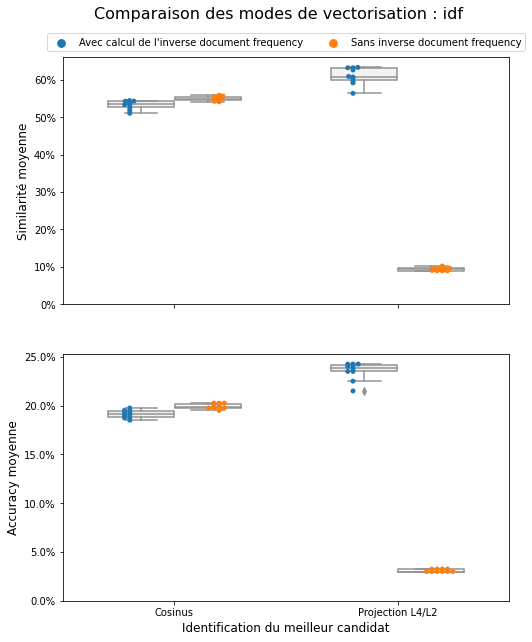
\includegraphics[width=0.9\linewidth]{img/tuning_idf.png}
                \end{center}
                \caption{Résultats du tuning de l'utilisation de l'inverse document frequency}
                \label{fig:tuning_idf}
            \end{figure}

            \subsubsection{Prise en compte des n-grams}

            La vectorisation des textes peut également être ajustée, en ajoutant en tant que features des ngrams de longueur variable.
            L'impact de la prise en compte de ngrams de plus en plus long (de 1 à 5 mots) est illustré à la \reffig{fig:tuning_ngrams}.

            On peut constater que :
            \begin{itemize}
                \item la prise en compte de ces ngrams a des effets mitigés dans le cas du cosinus
                \item elle est par contre bénéfique pour la projection, avec une saturation à partir des trigrammes
            \end{itemize}

            \begin{figure}[htbp]
                \begin{center}
                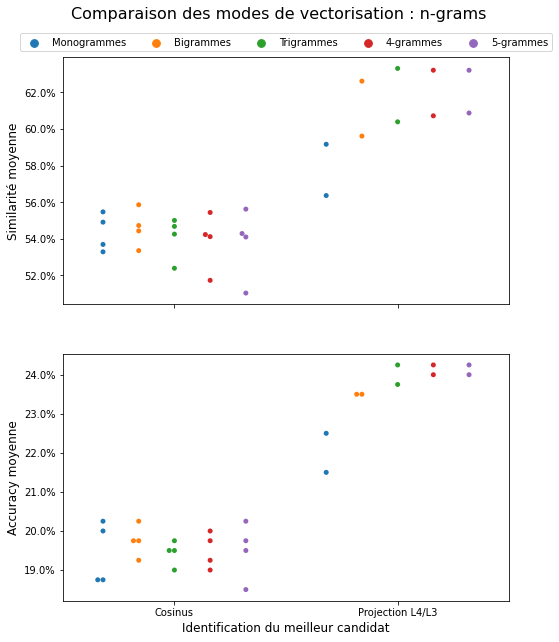
\includegraphics[width=0.9\linewidth]{img/tuning_ngrams.png}
                \end{center}
                \caption{Résultats du tuning de l'utilisation de l'inverse document frequency}
                \label{fig:tuning_ngrams}
            \end{figure}

            \subsubsection{Fonctions de scoring spécifique}

            Les fonctions de scoring \og absolu \fg et \og relatif \fg ont été présentée dans le chapitre sur l'analyse des données, à la section \mref{word_scores}.
            Elles permettent de calculer un score pour chaque mot, afin de quantifier son \og affinité \fg pour les listes d'ingrédients.
            L'utilisation d'un score relatif, qui peut être négatif (i.e. le mot concerné est plus souvent présent dans le corps du texte des documents que dans les listes d'ingrédients), et donc pénaliser le candidat. 
            C'est par exemple le cas du mot \og sel \fg, qui est évidemment un ingrédient mais qui est également très représenté par ailleurs dans le contenu des fiches techniques.
            L'utilisation de ces scores ne se peut se faire que pour la similarité cosinus, de la même manière qu'illustré à la \reffig{fig:similarite_score} (qui montre la \og négativité \fg du score du mot \og sel \fg).
            Il est même possible que la similarité du candidat avec le vecteur cible soit négative.

            \begin{figure}[htbp]
                \begin{center}
                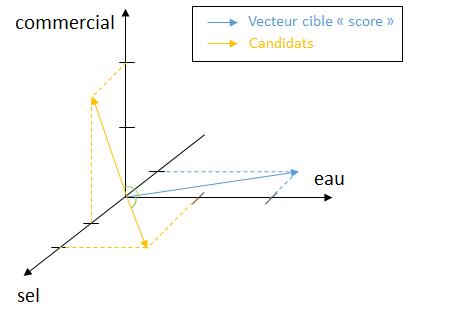
\includegraphics[width=0.6\linewidth]{img/similarite_score.png}
                \end{center}
                \caption{Illustration de la similarité cosinus avec score relatif}
                \label{fig:similarite_score}
            \end{figure}

            L'impact des fonctions de scoring a été illustré sur la base d'une grid search s'appliquant uniquement au mode d'identification cosinus, sans n-grams, avec retrait des stopwords et des accents.
            Elle fait varier :
            \begin{itemize}
                \item la comptabilisation des mots de manière binaire ou via les comptes
                \item la détermination ou non de l'inverse document frequency
                \item les scores : sans, avec le score absolu ou avec le score relatif
                \item les embeddings de mots : sans, Word2Vec, truncated SVD
            \end{itemize}
            Les résultats sont présentés à la \reffig{fig:tuning_score}.
            On constate que : 
            \begin{itemize}
                \item l'utilisation du score relatif dégrade très fortement la performance du modèle
                \item l'utilisation de l'idf avec le score absolu dégrade légèrement la performance
                \item le seul impact positif à l'utilisation d'une fonction de scoring est que score absolu améliore marginalement la performance en l'absence d'idf
            \end{itemize}
            La cause de la très faible performance du score relatif semble être la suivante : comme illustré précédemment à la \reffig{fig:relative_score_bar}, du fait de l'écart entre la taille des vocabulaires ingrédients et documents, les scores relatifs sont en moyenne négatifs.
            Par conséquent, plus ils sont longs, plus les vecteurs candidats ont en moyenne un produit scalaire négatif avec le vecteur cible.
            Ce qui signifie que le choix du meilleur candidat revient à prendre en compte le vecteur le moins négatif, voire un bloc de texte vide ou constitué de mots inconnus à l'entrainement\dots            

            \begin{figure}[htbp]
                \begin{center}
                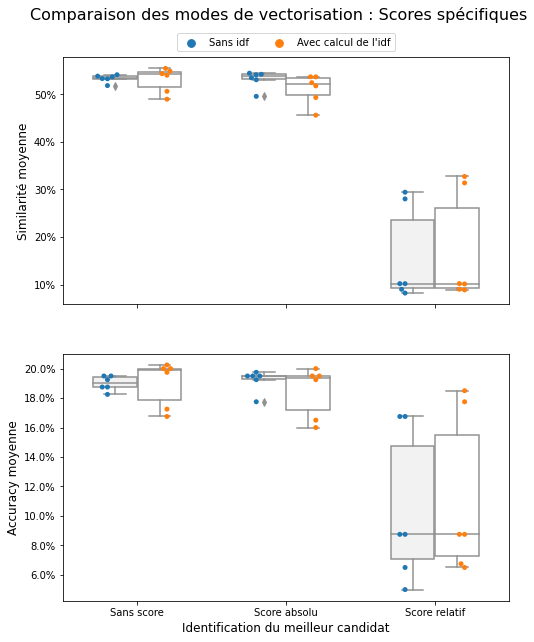
\includegraphics[width=0.6\linewidth]{img/tuning_score.png}
                \end{center}
                \caption{Illustration de la similarité cosinus avec score relatif}
                \label{fig:tuning_score}
            \end{figure}

            \subsection{Utilisation d'embeddings}

            L'utilisation d'embeddings a été évaluée via la même grid search que pour l'évaluation du scoring.
            Les résultats sont illustrés à la \reffig{fig:tuning_embedding}.
            On constate que : 
            \begin{itemize}
                \item les embeddings issus de la truncated SVD sous-performent par rapport aux autres méthodes (sans embeddings ou Word2vec)
                \item l'utilisation de Word2vec n'augmente globalement pas la performance du modèle
            \end{itemize}
            L'utilisation de ces embeddings, entraînés sur notre jeu de données uniquement, n'est pas concluant.

            \begin{figure}[htbp]
                \begin{center}
                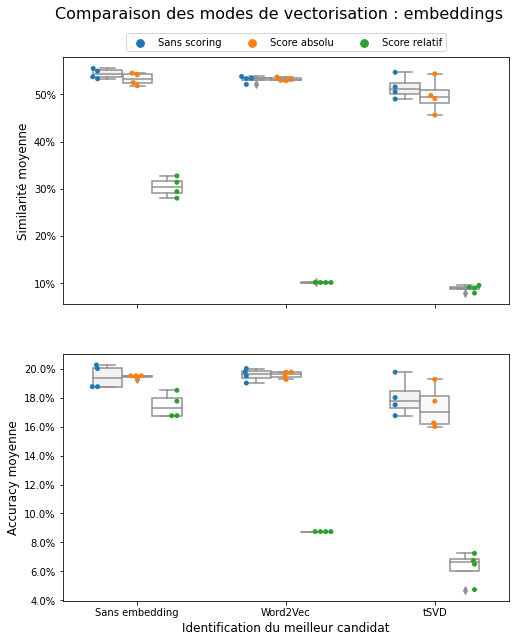
\includegraphics[width=0.6\linewidth]{img/tuning_embedding.png}
                \end{center}
                \caption{Illustration de la similarité cosinus avec score relatif}
                \label{fig:tuning_embedding}
            \end{figure}

            \section{\'{E}valuation finale de la performance}

            On peut tirer les enseignements suivants des travaux menés :
            \begin{itemize}
                \item des gains rapides on été obtenus en travaillant sur le preprocessing de base : stopwords, gestion des accents, découpage en blocs
                \item la similarité projection sur-performe nettement la similarité cosinus
                \item l'utilisations d'algorithmes plus complexes (embeddings et scoring) ne suffit pas à compenser cet écart de performance
            \end{itemize}

            Les paramètres ayant obtenu la meilleure performance ($63.31\% \pm 3.83\%$) sur la grid search sont : 
            \begin{itemize}
                \item similarité projection, avec les normes $L_{4}/L_{3}$
                \item retrait des stopwords, des accents
                \item découpage en blocs via la fonction 3 (avec expression régulière)
                \item vectorisation binaire des textes, sans appliquer l'inverse document frequency
                \item prise en compte des monogrammes, bigrammes et trigrammes
            \end{itemize}

            Si on entraîne un modèle avec ces paramètres sur le set d'entrainement, et qu'on évalue sa performance sur le set de test (qui n'a pas été utilisé lors du tuning des paramètres), on obtient les résultats suivants : 
            \begin{itemize}
                \item Similarité de Levenshtein moyenne : $67.18\%$
                \item Accuracy postprocessée : $27\%$
            \end{itemize}
            Ces résultats sont globalement bons, et illustrés en annexe à la \reftable{tbl:final_prediction}.
            Pour rappel, la performance initiale d'un modèle avant ajustement des paramètres était de $48.86\%$ (cf. \reftable{tbl:similarities_result}).
            Il apparaît que les principales améliorations passeraient par la mise en place de fonctions de découpage plus précises, de fonctionnalités de text postprocessing pour éliminer les préfixes, et d'OCR pour prendre en compte les documents numérisés.


\part{Travaux subséquents}
    \chapter{Opérationnalisation de cette maquette}    
        \section{Client et sponsor métier}
        \section{Définition des règles de gestion}
        \section{Mise en place d'une organisation projet}
        \section{Industrialisation du code}
        Prochaines étapes : opérationnalisation via API \\
        Documentation
        \section{Monitoring de la performance du modèle}
    \chapter{Extension des fonctionnalités offertes}
        \section{Prise en compte de nouveaux types de pièces jointes}
        \section{Utilisation d'outil d'OCR pour les pdf non structurés}
        \section{Mise en place d'outil de spatialisation des textes}
        \section{Construction d'outils d'extraction de données connexes à la composition}
        \section{\'{E}largissement aux données nutritionnelles}
        \section{Extraction d'informations complémentaires}
        \section{\'{E}valuation de la performances sur d'autres familles de produits}

\appendix
\part{Annexes}
    \chapter{Figures, tableaux et bibliographie}
        \listoftables
        \listoffigures
        \bibliographystyle{plain}
        \bibliography{./biblio} 
    \chapter{Exemples de pièces jointes et ground truth}
        \section{Fiches techniques}
        \label{ex:fiches_techniques}
        \includepdf[pages=1,
                    scale=0.8,
                    pagecommand={\subsection{Fiche technique sel Cerebos}\label{ex:FT_sel}}
                    ]
                    {doc_examples/FTF_8266604c-1ea2-47ca-a4fa-649b4147e733.pdf}
%        \includepdf[pages=2-,
%                    scale=1
%                    ]
%                    {doc_examples/FTF_8266604c-1ea2-47ca-a4fa-649b4147e733.pdf}

        \includepdf[pages=1,
                    scale=0.8,
                    pagecommand={\subsection{Fiche technique olives Valtonia}\label{ex:FT_olives}}
                    ]
                    {doc_examples/FTF_b7a5df3b-42b4-4cde-ae39-18f0e7a5f776.pdf}
%        \includepdf[pages=2-,
%                    scale=1
%                    ]
%                    {doc_examples/FTF_b7a5df3b-42b4-4cde-ae39-18f0e7a5f776.pdf}

        \includepdf[pages=1,
                    scale=0.8,
                    pagecommand={\subsection{Fiche technique Panna Cotta Nestlé}\label{ex:FT_pannacotta}}
                    ]
                    {doc_examples/FTF_d0aa2c1c-4317-4e5f-8a18-82e56976da22.pdf}
        \includepdf[pages=2-,
                    scale=0.8,
                    pagecommand={}
                    ]
                    {doc_examples/FTF_d0aa2c1c-4317-4e5f-8a18-82e56976da22.pdf}


        \includepdf[pages=1,
                    scale=0.8,
                    pagecommand={\subsection{Fiche technique confiture Andros}\label{ex:FT_confiture}}
                    ]
                    {doc_examples/FTF_e4c8c61f-a401-4384-8128-181447e5bdd2.pdf}
        \includepdf[pages=2-,
                    scale=0.8,
                    pagecommand={}
                    ]
                    {doc_examples/FTF_e4c8c61f-a401-4384-8128-181447e5bdd2.pdf}


        \includepdf[pages=1,
                    scale=0.8,
                    pagecommand={\subsection{Fiche technique ciboulette La case aux épices}\label{ex:FT_ciboulette}},
                    offset=0pt -15pt
                    ]
                    {doc_examples/FTF_eac17f96-1046-49c8-892d-a00220a75057.pdf}
        \includepdf[pages=2-,   
                    scale=0.8,
                    pagecommand={}
                    ]
                    {doc_examples/FTF_eac17f96-1046-49c8-892d-a00220a75057.pdf}
            
        \includepdf[pages=1,
                    scale=0.8,
                    pagecommand={\subsection{Fiche technique poivron El Arenal}\label{ex:FT_poivron}},
                    offset=0pt -15pt
                    ]
                    {doc_examples/FTF_a552d585-cb45-43bc-8fb9-1d208485d16c.pdf}
        \includepdf[pages=2-,   
                    scale=0.8,
                    pagecommand={}
                    ]
                    {doc_examples/FTF_a552d585-cb45-43bc-8fb9-1d208485d16c.pdf}
                    

        \includepdf[pages=1,
                    scale=0.8,
                    pagecommand={\subsection{Fiche technique mélange trappeur Terre Exotique}\label{ex:FT_meltrappeur}},
                    offset=0pt -15pt
                    ]
                    {doc_examples/FTF_e586f0d1-ae43-42ae-94db-b21ac515942e.pdf}            


% déclaration de la section incluse dans la première pagecommand
        \includepdf[pages=1,
                    scale=0.7,
                    pagecommand={\section{\'{E}tiquettes produit}\subsection{\'{E}tiquette curry Grain d'ailleurs}\label{ex:ET_curry}},
                    offset=0pt -25pt
                    ]
                    {doc_examples/ET_67d3ac42-64fe-4cc2-b728-923aba1a8d66.pdf}
 
        \includepdf[pages=1,
                    scale=0.7,
                    pagecommand={\subsection{\'{E}tiquette madeleines Saint Michel}\label{ex:ET_madeleine}}
                    ]
                    {doc_examples/ET_0481d91b-9653-42e7-b525-9dc9b87b06f2.pdf}

        \includepdf[pages=1,
                    scale=0.7,
                    pagecommand={\subsection{\'{E}tiquette lentilles Soufflet}\label{ex:ET_lentilles}}
                    ]
                    {doc_examples/ET_a57c1561-b88e-4694-8bd8-55623f2afa17.pdf}
        
        \includepdf[pages=1,
                    scale=0.7,
                    pagecommand={\subsection{\'{E}tiquette pannacotta Nestlé}\label{ex:ET_pannacotta}}
                    ]
                    {doc_examples/ET_d0aa2c1c-4317-4e5f-8a18-82e56976da22.pdf}
        
        \includepdf[pages=1,
                    scale=0.7,
                    pagecommand={\subsection{\'{E}tiquette sauce soja Kikkoman}\label{ex:ET_saucesoja}}
                    ]
                    {doc_examples/ET_f349e71d-fa03-41bc-8fa4-7e1c9c7f6d5b.pdf}

        \includepdf[pages=1,
                    scale=0.7,
                    pagecommand={\subsection{\'{E}tiquette mélange trappeur Terre Exotique}\label{ex:ET_meltrappeur}}
                    ]
                    {doc_examples/ET_e586f0d1-ae43-42ae-94db-b21ac515942e.pdf}

% déclaration de la section incluse dans la première pagecommand
        \includepdf[pages=1,
        scale=0.8,
        pagecommand={\section{\'{E}tiquetage manuel des données}\subsection{Règles de gestion pour l'étiquetage}\label{annotation_rules}},
        offset=0pt -25pt
        ]
        {doc_examples/annotation_rules.pdf}
        \includepdf[pages=2-,
        scale=0.9,
        pagecommand={}
        ]
        {doc_examples/annotation_rules.pdf}

%        \section{Ground truth}
        

%        {\renewcommand{\arraystretch}{2}%
%        \begin{table}[htbp]
%            {\scriptsize
%            \begin{center}%
%            \begin{longtable}{p{5cm}p{10cm}}
\toprule
                                                                                              designation &                                                                                                                                                                                                                                                                                                                                                                                                                                                                                                                                                                                                                                                                                                                                                                                                                                                                                                                                                                                                                              ingredients \\
\midrule
\endhead
\midrule
\multicolumn{2}{r}{{Continued on next page}} \\
\midrule
\endfoot

\bottomrule
\endlastfoot
                                                         Concentré liquide Asian en bouteille 980 ml CHEF &                                                                                                                                                                                                                                                                                                                                                                                                                                                                                                                                                                                                                                                                                                                                                                                                                                     Eau, maltodextrine, sel, arômes, sucre, arôme naturel de citronnelle, amidon modifié, ail en poudre, épices (combava, curcuma), extraits d'épices (gingembre, poivre), stabilisant (gomme xanthane). \\
                                                                    Pain burger curry 80 g CREATIV BURGER &                                                                                                                                                                                                                                                                                                                                                                                                                                                                                                                                                                                                                                                                                                                                                                                                                                                                                            Farine de blé T65, eau, levure, vinaigre de cidre, huile de colza, assaisonnement poudre de curry, sel, acide ascorbique, émulsifiant : E471. \\
                                                                         Macaroni en sachet 500 g PANZANI &                                                                                                                                                                                                                                                                                                                                                                                                                                                                                                                                                                                                                                                                                                                                                                                                                                                                                                 - 100\% Semoule de BLE dur de qualité supérieure  - Contient du gluten  Si le numéro de lot contient la lettre N : peu contenir de l'oeuf \\
                                                          Fève de Tonka en sachet 100 g COMPTOIR COLONIAL &                                                                                                                                                                                                                                                                                                                                                                                                                                                                                                                                                                                                                                                                                                                                                                                                                                                                                                                                          fève de tonka (graines ridées de 25 à 50mm de long)  Taux de coumarine compris entre 1 et 3,5 \% \\
                                                       Caviar d'aubergine en pot 500 g PUGET RESTAURATION &                                                                                                                                                                                                                                                                                                                                                                                                                                                                                                                                                                                                                                                                                                                                                                                                                                 Aubergine 60,5\% (aubergine, huile de tournesol), eau, oignon, huile de tournesol, jus de citron, concentré de tomate, huile d’olive vierge extra (2\%), ail, sel, persil, basilic, poivre, thym, romarin. \\
                                                          Confitures assorties en bocaux 30 g BONNE MAMAN &                                                                                                                                                                                                                                                                                                                                                            Confiture de myrtilles et de cassis  fruits (myrtilles 41\%, cassis 9\%), sucre, sucre roux de canne, jus de citrons concentré, gélifiant : pectine de fruits.  Confiture de fraises et de groseilles  fruits (fraises 27 \%, groseilles 23 \%), sucre, sucre roux de canne, jus de citrons concentré, gélifiant : pectine de fruits.  Confiture d'abricots et de pêches  fruits (abricots 34\%, pêches 16\%), sucre, sucre roux de canne, jus de citrons concentré, gélifiant : pectine de fruits.  Marmelade d'oranges douces et de mandarines  fruits (oranges douces 37\%, mandarines 3\%), sucre, sucre roux de canne, jus de citrons  concentré, gélifiant : pectine de fruits. \\
                                         Spécialité pomme saveur biscuitée en boîte 5/1 VALADE EN CORREZE &                                                                                                                                                                                                                                                                                                                                                                                                                                                                                                                                                                                                                                                                                                                                                                                                                                                                                                                                                             Pommes 95\%, sirop de glucose-fructose, arôme, antioxydant: acide ascorbique. \\
                                                                      Coco Pops en sachet 500 g KELLOGG'S &                                                                                                                                                                                                                                                                                                                                                                                                                                                                                                                                                                                                                                                                                                                                                                                                                                                                                                                       Riz, Sucre, Cacao maigre en poudre, Maltodextrine, Pâte de cacao, Sel, Arôme de malt d'orge, Arôme, Arôme naturel. \\
                                                                        PUR JUS ORANGE DE MÉDITERRANÉE 3L &                                                                                                                                                                                                                                                                                                                                                                                                                                                                                                                                                                                                                                                                                                                                                                                                                                                                                                                                                                                           jus d'orange issu de l'agriculture biologique. \\
                                                         Persil feuilles en boîte 80 g LA CASE AUX EPICES &                                                                                                                                                                                                                                                                                                                                                                                                                                                                                                                                                                                                                                                                                                                                                                                                                                                                                                                                                                                                                                   Persil \\
                                                         Chips saveur poulet braisé en sachet 25 g SIBELL &                                                                                                                                                                                                                                                                                                                                                                                                                                                                                                                                                                                                                                                                                                                   Pommes de terre, huile de tournesol (35\%), assaisonnement poulet (maltodextrine, farine de blé, dextrose, extrait de levure, arome, sel, oignon déshydraté, viande et graisse de poulet, ail, colorant : extrait de paprika E160c, Antioxydant : extrait de romarin E392), sel  Traces éventuelles de moutarde et lait \\
                                             Pâte à tartiner noisette en bouteille squeezer 1 kg CREPIOTE &                                                                                                                                                                                                                                                                                                                                                                                                                                                                                                                                                                                                                                                                                                                                         Sucre, huiles végétales ( Colza), noisettes (13\%), poudre de cacao maigre (7\%), lait écrémé en poudre , lactosérum en poudre, lactose. Emulsifiant lécithine de tournesol. Arôme : vanilline  Allergènes : Le produit peut contenir traces éventuelles de soja arachide et autre fruits a coque. \\
                                                          Sauce Sweet chili en flacon souple 875 ml HEINZ &                                                                                                                                                                                                                                                                                                                                                                                                                                                                                                                                                                                                                                                                                                                                                                                                                                                                                                               Sucre, eau, vinaigre d'alcool, purée de tomates mi-réduite, ail, amidon de maïs modifié, poivrons, piment 1,5\%, sel, épice \\
                                   PRÉPARATION CULINAIRE À BASE D'HUILE D'OLIVE ET D'ARÔME TRUFFE BLANCHE &                                                                                                                                                                                                                                                                                                                                                                                                                                                                                                                                                                                                                                                                                                                                                                                                                                                                                                                                                                                                  Huile d'olive vierge extra 99,5\%, Arôme \\
                                                  Huile pimentée spicy'piz en dose 3 ml SAVEURS ET SAUCES &                                                                                                                                                                                                                                                                                                                                                                                                                                                                                                                                                                                                                                                                                                                                                                                                                                                                                                                                                                                     Huile de colza, extrait naturel de piment de Cayenne \\
                                                                  Harissa en seau de 3 kg PROVENCE OLIVES &                                                                                                                                                                                                                                                                                                                                                                                                                                                                                                                                                                                                                                                                                                                                                                                                                                                                                                   Piment rouge fort équeuté* (85\%), cumin, ail moulu (3\%), eau, arome naturel d’ail, sel, sorbate de potassium. (* présence de sulfites) \\
                                                                                      1883 VANILLE 100 CL &                                                                                                                                                                                                                                                                                                                                                                                                                                                                                                                                                                                                                                                                                                                                                                                                                                                                                                                                                                 SUCRE DE CANNE, EAU, AROME, COLORANT : E 150a, AROME NATUREL DE VANILLE. \\
                                                            Baie des Batak en sachet 250 g TERRE EXOTIQUE &                                                                                                                                                                                                                                                                                                                                                                                                                                                                                                                                                                                                                                                                                                                                                                                                                                                                                                                                                                                                                           Baie des Batak \\
                                              Filet de maquereau à la tomate en poche 4/4 FURIC SAUPIQUET &                                                                                                                                                                                                                                                                                                                                                                                                                                                                                                                                                                                                                                                                                                                                                                                                                                                        Filets de maquereaux (61 \%), eau, concentré de tomate (15\%), huile de tournseol, vinaigre d'alcool, vinaigre de vin blanc, sel, vin blanc, épaississant : gomme xanthane, arômes. \\
                                                 Farine de blé type 00 pour pizza en sachet 1 kg SOUFFLET &                                                                                                                                                                                                                                                                                                                                                                                                                                                                                                                                                                                                                                                                                                                                                                                                                                                                                                                                                                                    Mélange de Blés de pays recommandés par la meunerie . \\
                                                            GOURDES AU CHOCOLAT P'TITS TOQUES YABON 4X80G &                                                                                                                                                                                                                                                                                                                                                                                                                                                                                                                                                                                                                                                       Lait entier (88\%) ; sucre ; poudre de chocolat (3.1\%) (sucre, poudre de cacao) ; amidon modifié de manioc ; chocolat au lait (0,57\%) (sucre, pâte de cacao, poudre de lait entier, beurre de cacao, poudre de lait écrémé) ; arôme naturel ; épaississants : gomme gellane, gomme guar ; correcteur d'acidité : citrate tri-sodique ; concentré de minéraux du lait ; vitamine D3. \\
                                                                                          CHAMONIX*2 25G  &                                                                                                                                                                                                                                                                                                                                                                                                                                                                                                                                                                                                                        Sirop de glucose-fructose, farine de BLÉ , sucre, purée d'orange 5,4 \%, jus d'orange concentré 1,5 \% (équivalent jus d'orange 8 \%), huile de colza, jaunes d' OEUFS en poudre, stabilisant (glycérol), poudre à lever (carbonate acide d'ammonium), gélifiant (pectines), acidifiant (acide citrique), arômes, colorant (rocou), conservateur (sorbate de potassium). PEUT CONTENIR LAIT, FRUITS À COQUE, SÉSAME. \\
                                           Thon Albacore en morceaux au naturel en poche 1,95 kg LA PULPE &                                                                                                                                                                                                                                                                                                                                                                                                                                                                                                                                                                                                                                                                                                                                                                                                                                                                                                                                                                                                  Thon Albacore (92\%), eau (7\%), sel (1\%) \\
                                                                                THE BISCUITS POCKET 22 GR &                                                                                                                                                                                                                                                                                                                                                                                                                                                                                                                                                                                                                                                                                                                                                          Farine de BLÉ 67 \%, sucre, huile de palme, sirop de glucose-fructose, LAIT écrémé en poudre, lactosérum en poudre (de LAIT), arôme fleur d'oranger, fibres de BLÉ, sel, poudre à lever (carbonates de sodium, carbonates d'ammonium), émulsifiant (lécithines de SOJA), arômes. \\
                                          Galette des rois à la crème frangipane avec fève 400 g PASQUIER &                                                                                                                                                                                                                                                                                                                                                                                                                                                                                                                                           Crème frangipane 39\% (sucre, BEURRE pâtissier, AMANDES en poudre 5,8\%, eau, farine de BLE, OEUFS frais, poudre de LAIT  écrémé, poudres à lever: diphosphates et carbonates de sodium, arôme naturel) - Farine de BLE - BEURRE pâtissier - Eau - Lactoserum (LAIT) et  protéines de LAIT - OEUFS frais - Sel - Agent de traitement de la farine: L-cystéine.  Ce produit contient : BEURRE, AMANDES, BLÉ, OEUFS, LAIT.  Ce produit a pu être en contact avec : Arachide, Soja, Fruits à coque. \\
                                                                         COLIS KERMESSE 2019  A.P " 22+8" &  TAGADA  sucre; sirop de glucose; gélatine; acidifiant: acide citrique; arôme; colorants: curcumine, carmins, carotènes végétaux.  DRAGIBUS SO  sirop de glucose; sucre; amidon; dextrose; acidifiants: acide citrique, acide malique; correcteurs d'acidité: citrate monosodique, malate acide de sodium; arôme; colorants: curcumine, bleu patenté V, charbon végétal, carotènes végétaux, anthocyanes; agent d'enrobage: cire de carnauba.  HAPPY COLA  sirop de glucose; sucre; gélatine; dextrose; acidifiant: acide citrique; sirop de caramel; arôme; agents d'enrobage: cire d'abeille blanche et jaune, cire de carnauba.  MAO CROQUI  sucre; sirop de glucose; graisse de palme; humectant: sirop de sorbitol; acidifiant: acide citrique; gélatine; arôme; concentrés de fruits et de plantes: citron, carthame, spiruline, cassis, carotte, radis, pomme; correcteur d'acidité: carbonate acide de sodium; agent d'enrobage: cire d'abeille blanche et jaune; antiagglomérant: talc; sirop de sucre  nverti. Tenir à  l'a... \\
                                             Ice Tea citron-citron vert en bouteille 50 cl LIPTON ICE TEA &                                                                                                                                                                                                                                                                                                                                                                                                                                                                                                                                                                                                                                                                                                                                                                                                                                         eau  sucre  etrait de thé noir (1,4g/l)  acidifiant (acide citrique)  jus de citron à base de concentré (0,1\%)  arôme  correcteur d'acidité (citrate trisodique)  antioxydant (acide ascorbique) \\
                                                                    Couscous blanc BIO en sac 5 kg MARKAL &                                                                                                                                                                                                                                                                                                                                                                                                                                                                                                                                                                                                                                                                                                                                                                                                                                                                                                                                                                                               semoule de blé dur blanche biologique, eau \\
                                                    Feuilles de vigne farcies au riz en boîte 2/1 ONASSIS &                                                                                                                                                                                                                                                                                                                                                                                                                                                                                                                                                                                                                                                                                                                                                                                                                                                                 Riz à grain long précuit (65\%), feuilles de vignes (15\%), eau, huile de soja (10\%), oignons, aneth, menthe, sel, condiments, agent correcteur d’acidité : acide citrique \\
                                        Spécialité au citron en bouteille verre 70 cl PULCO PROFESSIONNEL &                                                                                                                                                                                                                                                                                                                                                                                                                                                                                                                                                                                                                                                                                                                                                                                                                                                       jus de fruits à base de concentrés : citron 54,6\% et orange 4,4\% (équivalent à 59\% de jus reconstitués), eau, pulpes de citron 5\%, acidifiant : acide citrique, extrait de citron. \\
                                         Olives vertes piquantes dénoyautées en seau 3,5 kg DE NOTEKRAKER &                                                                                                                                                                                                                                                                                                                                                                                                                                                                                                                                                                                                                                                                                                                                           Olives vertes 98\%denoyautées , huile tournesol, piments, sel ,poivre,(cayenne,noire) acides (citrique,LACTIQUE,ascorbique), paprika rouge, poireau, oignon, persil, ail, tomate, bouillon (hydrolysat de protéines, SOYA et maïs, graisse de palme RPSO), noix de muscade, Conservateur :E220. \\
                                                           Mélange d'épices italien en boîte 200 g DUCROS &                                                                                                                                                                                                                                                                                                                                                                                                                                                                                                                                                                                                                                                                                                                                                                                                                           Poivrons rouge et vert, tomate en poudre, ail déshydraté (14,9\%), origan (11,8\%), oignon déshydraté, marjolaine (5\%), paprika, basilic, poivre noir, huile de tournesol, antiagglomérant: dioxyde de silicium. \\
                                                           Entremet parfum caramel en sachet 1 kg NUTRACY &                                                                                                                                                                                                                                                                                                                                                                                                                                                                                                                                                                                                                                                                                                                                                                                                                                                                                                                 Sucre, texturants : alginate de sodium, carraghénane, colorant : caramel E150c, arôme, amidon modifié de pomme de terre. \\
                                                          Crème de cèpes a la truffe en boîte 4/4 DEMETRA &                                                                                                                                                                                                                                                                                                                                                                                                                                                                                                                                                                                                                                                                                                                                          cèpes 70\% (Boletus edulis et respective famille), huile de tournesol, blanquette 5\% (Tuber borchii Vitt.), oignon, beurre, sel, protéines du lait, farine de riz, amidon de mais, dextrose, extrait de levure, épices, arôme truffée, arômes naturels, antioxydant: acide l-ascorbique (E 300). \\
                                                    Sauce dessert fraise en bouteille 1 kg NESTLÉ DOCELLO &                                                                                                                                                                                                                                                                                                                                                                                                                                                                                                                                                                                                                                                                                                                                                                                                                              Sirop de glucose, purée de fraises (21\%), sirop de sucre inverti, sucre, arôme, amidon modifié, acidifiant (acide citrique), épaississant (pectines), conservateur (sorbate de potassium), colorant (E120). \\
                                                                  Mini marshmallows en boîte 150 g VAHINE &                                                                                                                                                                                                                                                                                                                                                                                                                                                                                                                                                                                                                                                                                                                                                                                                                                                                                                                                Sirop de glucose-fructose, sucre, eau, gélatine (de porc), amidon de maïs, arôme, colorants : E100, E120. \\
                                                                           Moutarde en stick 10,5 g HEINZ &                                                                                                                                                                                                                                                                                                                                                                                                                                                                                                                                                                                                                                                                                                                                                                                                                                                                               Eau, graines de moutarde 16\%, vinaigre, vinaigre de malt (orge),sucre, sel, miel, épices, arôme naturel, épaississant (gomme xathane), extrait de paprika. \\
                                                          Entremet parfum vanille en sachet 750 g NUTRACY &                                                                                                                                                                                                                                                                                                                                                                                                                                                                                                                                                                                                                                                                                                                                                                                                                                                              Sucre, gélifiant : alginate de sodium, maltodextrine de maïs, arômes, épaississant : carraghénane, amidon modifié de pomme de terre, huile de tournesol, colorant : E101ii. \\
                                                 Thon listao en morceaux au naturel en boîte 4/4 LMC FOOD &                                                                                                                                                                                                                                                                                                                                                                                                                                                                                                                                                                                                                                                                                                                                                                                                                                                                                                                                                                                                                           Thon, eau, sel \\
                                                                 Nappage miroir neutre en seau 7 kg ANCEL &                                                                                                                                                                                                                                                                                                                                                                                                                                                                                                                                                                                                                                                                                                                                                                                                                                                                                                                        Sirop de glucose, sucre, eau, stabilisants (E440i, E440ii, E415), acidifiants (E330, E450i), conversateur (E202). \\
                                                                    Sauce diable en boîte 800 g NEFF MADA &                                                                                                                                                                                                                                                                                                                                                                                                                                                                                                                                                                                                                                                                                                                 Maltodextrine de blé - Amidon de maïs - Sel - Amidon de pomme de terre - Echalote - Arômes - Sucre - Sirop de glucose de maïs - Tomate - Oignon grillé - Extrait de levure - Huile de colza - Extrait naturel de vinaigre d'alcool - Colorant : E150c - Acidifiant : E330 - Extrait naturel de vin blanc - Ail - Epices. \\
                                                        Purée de cassis sucrée en poche 1 kg LEONCE BLANC &                                                                                                                                                                                                                                                                                                                                                                                                                                                                                                                                                                                                                                                                                                                                                                                                                                                                                                                        Cassis 89,3\%*1, sucre.  *1 : Variable selon la teneur en sucre initiale du fruit à sa récolte. Tolérance de ± 3\%. \\
                                                                      Oasis orange en bouteille 2 L OASIS &                                                                                                                                                                                                                                                                                                                                                                                                                                                                                                                                                                                                                                                                                                                                                                                                                           eau de source 80\%, jus de fruits à base de concentrés 12 \% (orange 10 \%, pomme), sucre, acidifiants : acide citrique et acide malique, arômes, antioxydant : acide  ascorbique, colorant : extrait de paprika. \\
                                                                      Muffin Gourmet en sac 10 kg COMPLET &                                                                                                                                                                                                                                                                                                                                                                                                                                                                                                                                                                                                                                                                                                                                                                                                  Sucre, amidon de FROMENT, farine de FROMENT, amidon modifié, fibres solubles, poudre à lever : (E450, E500, E341), poudre de LAIT écrémé, émulsifiants : (E471, E472e),  amidon, farine de FROMENT pré gélatinisée, sel, arôme naturel. \\
                                                                     Miso en poudre en boîte 250 g ARIAKE &                                                                                                                                                                                                                                                                                                                                                                                                                                                                                                                                                                                                                                                                                                                                                                                                                                                                                                                 Miso (95\%) (eau, fèves de soja, riz, sel), extrait de levure, bonite (poisson), fibre de soja.  Contient : poisson, soja \\
                                                      Tarte sablée sucrée au beurre en forme de cœur PIDY &                                                                                                                                                                                                                                                                                                                                                                                                                                                                                                                                                                                                                                                                                                                                                                                       farine de BLE enrichie (farine de BLE, farine d'ORGE maltée, vitamine B1 \& B2, nicotinamide, acide folique, fer), BEURRE 26.73\%, sucre, OEUF, sirop de sucre inverti, sel  Fabriqué dans une usine utilisant des FRUITS à COQUE, SOJA et ARACHIDES \\
                                                                Beignet au beurre en sachet 10 kg COMPLET &                                                                                                                                                                                                                                                                                                                                                                                                                                                                                                                                                                                                                                                                                                                                                                                                                     Farine de blé, beurre en poudre (7 \%), sucre, émulsifiants, sel, dextrose, poudre de blancs d'oeufs, lactose, gluten de blé, poudre à lever : (E450, E500), arôme, antioxygène : E300, alpha amylase, hémicellulase. \\
                                                               Semoule de blé fine BIO en sac 5 kg MARKAL &                                                                                                                                                                                                                                                                                                                                                                                                                                                                                                                                                                                                                                                                                                                                                                                                                                                                                                                                                                                                     blé dur biologique (triticum durum). \\
                                                   Jus de rôti de boeuf hyposodé en boîte 800 g NEFF MADA &                                                                                                                                                                                                                                                                                                                                                                                                                                                                                                                                                                                                                                                                                                                                                                                                                                                                         Amidon de maïs - Arômes - Sirop de glucose de maïs - Huile de colza - Sucre - Oignon grillé - Extrait de levure - Colorant : E150c - Ail - Viande de bœuf 0,4 \%. \\
                                                     Moutarde forte de Dijon en tube 105 g REINE DE DIJON &                                                                                                                                                                                                                                                                                                                                                                                                                                                                                                                                                                                                                                                                                                                                                                                                                                                                                                                              Eau, graines de moutarde, vinaigre d'alcool, sel, acidifiant (acide citrique), antioxydant E 224 (sulfite). \\
                                                                      Céleri râpé en boîte 5/1 EPISAVEURS &                                                                                                                                                                                                                                                                                                                                                                                                                                                                                                                                                                                                                                                                                                                                                                                                                                                                                                                                                                     Céleri rave, eau, vinaigre d´alcool, sel, sucre et antioxydant: E300 \\
                                                                            CHEDDAR CHEESE SAUCE 1.420 KG &                                                                                                                                                                                                                                cheddar fondu (44\%) (eau, lactosérum, cheddar (5\%) (lait, ferments, acidifiant (sulfates de sodium (E514)), enzymes), lait écrémé, maltodextrine, antioxydant (phosphate de sodium (E339)), crème, épaississants (octényle succinate d'amidon sodique (E1450), gomme xanthane (E415)), acidifiant (sulfates de sodium (E514))), eau, huile de palme, épaississants (amidon modifié de tapioca, amidon modifié de maïs), maltodextrine, acidifiants (sulfates de sodium (E514), citrate de sodium (E331), acide phosphorique (E338), acide lactique (E270)), arôme, antioxydant (phosphate de sodium (E339)), colorants (bêta carotène (E160a), annatto (E160b), extrait de paprika (E160c)), émulsifiants (stéaroyl-2-lactylate de sodium (E481), mono et diglycérides d'acides gras alimentaires (E471)) \\
                                                          Brandade de morue en boîte 5/1 RAYMOND GEOFFROY &                                                                                                                                                                                                                                                                                                                                                                                                                                                                                                                                                                                                                                                                                                                                                                                                                                                                                                                        Huile de colza, morue (32\%), eau, protéines de lait, sel, épaississant : carraghénanes (extrait d’algues marines) \\
                                                                   OLIVES NOIRES CONFITES DENOYAUTEES 4/4 &                                                                                                                                                                                                                                                                                                                                                                                                                                                                                                                                                                                                                                                                                                                                                                                                                                                                                                                                                                                        Olives, eau, sel, stabilisateur de couleur : E579 \\
                                                                  Sauce algérienne en flacon 850 g COLONA &                                                                                                                                                                                                                                                                                                                                                                                                                                                                                                                                                                                                                                                                                             Huile de colza (48 \%), sucre, eau, vinaigre, purée de tomates, jaunes d’oeufs (4.4 \%), oignons, moutarde (eau, graines de moutarde, sel, vinaigre, curcuma), extraits naturels et aromates, oignons rôtis (1.6 \%) (contient blé), sel, antioxydant : extrait de romarin, acidifiant : acide citrique, arômes, colorant : extrait de paprika. \\
                                                               Ketchup en flacon souple 970 ml CALIFORNIA &                                                                                                                                                                                                                                                                                                                                                                                                                                                                                                                                                                                                                                                                                                                                                                                                                                                                                                                                     Purée de tomates mi réduite (64\%), sucre, vinaigre, amidon modifié, sel, acidifiant : acide citrique \\
                                                                 Protéine de soja BIO en sac 10 kg MARKAL &                                                                                                                                                                                                                                                                                                                                                                                                                                                                                                                                                                                                                                                                                                                                                                                                                                                                                                                                                                                                      soja jaune biologique (glycine max) \\
                                       Spécialité pomme-abricot allégée en coupelle 95 g CHARLES ET ALICE &                                                                                                                                                                                                                                                                                                                                                                                                                                                                                                                                                                                                                                                                                                                                                                                                               Pomme 77\% (origine 100\% France), abricot 20\% (origine 100\% France), sucre (origine 100\% France), jus concentré de carotte, antioydant: acide ascorbique.  Certains ingrédients de ce produit de proviennent pas de France. \\
                                                                          Barre pâtissière 800 g COQUELIN &                                                                                                                                                                                                                                                                                                                                                                                                                                                                                                                                                                                                                                                                                                                                       Farine de BLÉ - Sucre - OEUFS - Huile de colza - Eau - Blancs d'OEUFs - Sirop de glucose déshydraté - Poudres à lever: diphosphates, carbonates de sodium - Sel - Conservateur : sorbate de potassium - Correcteur d'acidité : acide citrique - Arômes (contient alcool) - colorant : caroténoïdes \\
                                                              Compote poire allégée en boite 5/1 LA PULPE &                                                                                                                                                                                                                                                                                                                                                                                                                                                                                                                                                                                                                                                                                                                                                                                                                                                                                                                                           Poires, sirop de glucose-fructose, acidifiant : acide citrique, antioxydant: acide ascorbique. \\
                                                                      Pois chiches en boîte 1/2 MAINGOURD &                                                                                                                                                                                                                                                                                                                                                                                                                                                                                                                                                                                                                                                                                                                                                                                                                                                                                                                                                                                                                  Pois chiches, eau, sel. \\
                                                      Bâton chocolat noir 40\% cacao en boîte 1,6 kg CEMOI &                                                                                                                                                                                                                                                                                                                                                                                                                                                                                                                                                                                                                                                                                                                                                                                                                                                                                                                    sucre, pâte de cacao, beurre de cacao, émulsifiant : lécithine de tournesol (E322), arôme vanille  cacao : 40\%minimum \\
                                                            Potage aux 9 légumes en sachet 20 g NEFF MADA &                                                                                                                                                                                                                                                                                                                                                                                                                                                                                                                                                                                                                                                                                                               Amidon modifié de pomme de terre - Légumes 34,75 \% (pomme de terre, tomate, céleri, pois vert, carotte, oignon, chou-fleur, poireau, épinard) - Sirops de glucose de maïs et de blé - Arômes naturels - Matières grasses végétales : Huile de tournesol, huile de colza - Sucre - Sel - Ail - Protéines de lait - Curcuma. \\
                                                                           Pancake en sachet 1 kg COMPLET &                                                                                                                                                                                                                                                                                                                                                                                                                                                                                                                                                                                                                                                                                                                                                                                                                                          Farine de FROMENT, poudre de LACTOSERUM, sucre, poudre d'OEUF entier, poudres à lever: (E450, E500), matière grasse LAITIERE, sel.  Peut contenir des traces de : soja, fruits à coques, lupin. \\
                                                    Mirabelle dénoyautée au naturel en boîte 2/1 ODENWALD &                                                                                                                                                                                                                                                                                                                                                                                                                                                                                                                                                                                                                                                                                                                                                                                                                                                                                                                                                       Mirabelles (55\%), eau, acidifiant : acide citrique, antioxydant : acide ascorbique \\
                    Soupe de poissons et langoustines au sel de Guérande en boite en boîte 3/1 BEAUMOULIN &                                                                                                                                                                                                                                                                                                                                                                                                                                                                                                                                                                                                                                                                                                                                                                  Eau, poissons 35\%, langoustines 5\% (têtes et pattes), purée de tomates double concentrée, amidon modifié de maïs, oignons, carottes, poireaux, vin blanc, sel de Guérande 1.45\%, épices et plantes aromatiques, huile d’olive vierge extra, arôme naturel de crustacés. \\
        PRÉPARATION DÉSHYDRATÉE POUR FLAN 5 PARFUMS ÉDULCORÉ À L'ASPARTAME À CHAUD EN SACHET 150 G ANEPIA &  FRAMBOISE  Maltodextrine, carraghénane E407a, amidon de blé, colorant : jus concentré de betterave E162, édulcorant : aspartame E951* (0.37\%), arôme goût framboise (substances aromatisantes, substances aromatisantes naturelles).   *Contient une source de phénylalanine, ne convient pas aux femmes enceintes.  CAFE  Maltodextrine, café soluble (3.6\%), carraghénane E407a, amidon de maïs, colorant : caramel E150d, édulcorant : aspartame E951* (0.38\%), arôme goût café (substances  aromatisantes).  *Contient une source de phénylalanine, ne convient pas aux femmes enceintes.  PISTACHE  Maltodextrine, carraghénane E407a, amidon de blé, arôme goût pistache (préparations aromatisantes, substances aromatisantes, substances aromatisantes naturelles),  colorants : extrait de curcuma E100 (0.0017\%) et chlorophylle E141, édulcorant : aspartame E951* (0.35\%).  *Contient une source de phénylalanine, ne convient pas aux femmes enceintes.  CACAO  Maltodextrine, cacao (15\%), amidon de blé, carraghénane... \\
                                                         Saladière parisienne en coupelle 220 g SAUPIQUET &                                                                                                                                                                                                                                                                                                                                                                                                                                                                                                                                                                                                                                                                       Légumes (pommes de terre (14\%), carottes (10\%), champignons (9\%), haricots verts, persil), sauce, thon* (22\%).  Composition de la sauce : Eau, huile de tournesol, vinaigre, moutarde de Dijon (eau, graines de moutarde, vinaigre, sel), sel, arômes, amidons transformés de maïs, épaississants : gomme guar et gomme xanthane.  *Euthynnus (Katsuwonus) pelamis \\
                                                  San Pellegrino Limonata en canette 33 cl SAN PELLEGRINO &                                                                                                                                                                                                                                                                                                                                                                                                                                                                                                                                                                                                                                                                                                                                                                                                                                                                                                                                                                                                                                        - \\
                                                     Chapelure Batter Mix en sac de 4,2 kg GRIFFITH FOODS &                                                                                                                                                                                                                                                                                                                                                                                                                                                                                                                                                                                                                                                                                                                                                                                                                                                                                                                                                                                                                                        - \\
                                            SPÉCIALITÉ POMME-FRAISE ALLÉGÉE EN SUCRES EN BOÎTE 5/1 VALADE &                                                                                                                                                                                                                                                                                                                                                                                                                                                                                                                                                                                                                                                                                                                                                                                              Pommes 89\%, purée de fraises à base de concentré 6\% , sirop de glucose-fructose, arôme naturel, jus concentré de carotte pourpre, antioxydant : acide ascorbique, acidifiant : acide citrique (si le fruit n'en contient pas suffisamment). \\
                                                               MOUTARDE DE DIJON SEAU 5KG - EDMOND FALLOT &                                                                                                                                                                                                                                                                                                                                                                                                                                                                                                                                                                                                                                                                                                                                                                                                                                                                                                                       Eau, graines de moutarde, vinaigre, sel, antioxydant : disulfite de potassium, acidifiant : acide citrique, épice. \\
                                                       Assortiment Mix Turbine 3 saveurs en colis MONBANA &  Croustilles de céréales enrobées de chocolat au lait et de chocolat blanc arôme café  chocolat blanc arôme café 48\% (sucre, beurre de cacao, poudre de lait entier, arômes), chocolat au lait 38\% (sucre, beurre de cacao, poudre de lait entier, pâte de cacao, émulsifiant : lécithines (soja), arôme naturel de vanille), céréales croustillantes 12\% (farine de blé, gluten de blé, sucre, farine de malt de blé, poudre à lever : E500(ii), sel, correcteur d’acidité : E170), sucre glace.   Chocolat au lait et blanc: cacao 33\% min. Traces éventuelles de : oeufs, fruits à coque.  Croustilles de céréales enrobées de chocolat au lait et de pâte de spéculoos  chocolat au lait 68\% (sucre, beurre de cacao, poudre de lait entier, pâte de cacao, émulsifiant : lécithines (soja), arôme naturel de vanille), pâte de spéculoos 16\% [Spéculoos 60\% (farine de blé, sucre, huiles et graisses végétales (palme, colza), sirop de candi, poudres à lever : E500(ii) - carbonate acide d'ammonium, sel, cannelle), huiles ... \\
                                                              Lentilles blondes en sac 5 kg VIVIEN PAILLE &                                                                                                                                                                                                                                                                                                                                                                                                                                                                                                                                                                                                                                                                                                                                                                                                                                                                                                                                                                                                                        Lentilles blondes \\
                                                                                CÉLÉBRATIONS EN ÉTUI 69 G &                                                                                                                                                                                                                                                                                                                                                                                                                                                                 Sucre, sirop de glucose, beurre de cacao, lait écrémé en poudre, pâte de cacao, matière grasse du lait, lactose, farine de blé, matière grasse de palme, cacahuètes, noix de coco séchée, petit-lait en poudre, huile de palme, lait entier en poudre, huile de tournesol, émulsifiants (lécithine de soja, E471), extrait de malt d'orge, cacao maigre, sel, humectant (glycérol), blanc d'oeuf en poudre, extrait naturel de vanille, poudres à lever (E341, E500, E501), protéine de lait, gluten de blé. (Peut contenir: noisette, amande, avoine).Cacao 25\% minimum \\
                                                                Jus d'orange en bouteille brique 1 L BOPI &                                                                                                                                                                                                                                                                                                                                                                                                                                                                                                                                                                                                                                                                                                                                                                                                                                                                                                                                                                                                         Jus d’orange à base de concentré \\
                                               Farine de pois chiche en sachet 1 kg HEUSCHEN AND SCHROUFF &                                                                                                                                                                                                                                                                                                                                                                                                                                                                                                                                                                                                                                                                                                                                                                                                                                                                                                                                                                                                                    Farine de pois chiche \\
                                                                  HARICOTS BLANCS BIO 2.5KG VIVIEN PAILLE &                                                                                                                                                                                                                                                                                                                                                                                                                                                                                                                                                                                                                                                                                                                                                                                                                                                                                                                                                                                        Haricots blancs issus de l'Agricutlure Biologique \\
                                                                   GNOCCHI SARDI ANTONIO AMATO SAC DE 3KG &                                                                                                                                                                                                                                                                                                                                                                                                                                                                                                                                                                                                                                                                                                                                                                                                                                                                                                                                                                                                semoule de blé dur supérieure et de l'eau \\
                                                  Cocktail de fruits au sirop léger en boîte 5/1 ST MAMET &                                                                                                                                                                                                                                                                                                                                                                                                                                                                                                                                                                                                                                                                                                                                                                                                         Pêches et poires en cubes (avec leur jus d'origine naturelle 6,25\%*), segments d'ananas, raisins, eau, sirop de glucose-fructose, sucre, arôme naturel, acidifiant : acide citrique.  *Sur une base de 100\% de pêches et poires. \\
                                                                         Pulpe d'ail en pot 1 kg SOKODAIL &                                                                                                                                                                                                                                                                                                                                                                                                                                                                                                                                                                                                                                                                                                                                                                                                                                                                                                                                                Ail réhydraté (91\%) - Origine : Chine. Sel, Acide citrique E330. Disulfite de sodium E223 \\
                                                                    Céleri garniture en boîte 5/1 ARAMAYO &                                                                                                                                                                                                                                                                                                                                                                                                                                                                                                                                                                                                                                                                                                                                                                                                                                                                                                          Garniture de celeri, eau, sel  GARNITURE DE CELERI RO-4250: origine Espagne.Garniture de celeri: 58,95\%, eau: 39,45\%, sel: 0,6\% \\
                                                               Coca-Cola light en canette 15 cl COCA COLA &                                                                                                                                                                                                                                                                                                                                                                                                                                                                                                                                                                                                                                                                                                                                                                                                                                              eau gazéifiée  colorant : E150d  acidifiants : acide phosphorique, acide citrique  édulcorants : aspartame, acésulfameK  arômes naturels dont caféine  contient une source de phénylalanine \\
                                                                        Galletti en paquet 500 g DE CECCO &                                                                                                                                                                                                                                                                                                                                                                                                                                                                                                                                                                                                                                                                                                                                                                                                                                                                                                                                                                                                SEMOULE DE BLE' DUR de qualité supérieure \\
                                                            Lait écrémé en poudre en sachet 500 g MATINES &                                                                                                                                                                                                                                                                                                                                                                                                                                                                                                                                                                                                                                                                                                                                                                                                                                                                                                                                                               Poudre de lait écrémé, anti-agglomérant : E551 [nano]  Lait origine France \\
                                      Assortiment de Malabar magic blue 3 parfums en boîte de 300 MALABAR &                                                                                                                                                                                                                                                                                                                                                                                                                                                                                                                                                                                                                                                                                                                                                                                                                                                       Sucre, Gomme base, Sirop de glucose, Acidifiant (E330), Humectants (E422, E1518), Arômes, Emulsifiant (Lécithine de tournesol), Colorants (E150a, E133, E120), Antioxydant (E321). \\
                                                            CONFITURE DE FRAMBOISES 4/4 VALADE EN CORRÈZE &                                                                                                                                                                                                                                                                                                                                                                                                                                                                                                                                                                                                                                                                                                                                                                                                                                                                                                                                     Sirop de glucose-fructose, framboises 35\%, sucre, gélifiant : pectines, acidifiant : acide citrique. \\
                                                        Câpres surfines au vinaigre en boîte 4/4 MARTIN'S &                                                                                                                                                                                                                                                                                                                                                                                                                                                                                                                                                                                                                                                                                                                                                                                                                                                                                                                                                                                                               Câpres, eau, vinaigre, sel \\
                                                                   Sel fin en sac 10 kg SALINE D'EINVILLE &                                                                                                                                                                                                                                                                                                                                                                                                                                                                                                                                                                                                                                                                                                                                                                                                                                                                                                                                                                                                        sel, antiagglomérant E536 ou E535 \\
                                     Compote pomme-abricot allégée en coupelle 100 g LE BERGER DES FRUITS &                                                                                                                                                                                                                                                                                                                                                                                                                                                                                                                                                                                                                                                                                                                                                                                                                                                                                                                                                                          Pommes 70\%, abricots 25\%, sucre, antioxydant: acide ascorbique. \\
                                                                        RIZ ETUVE BIO IGP DE CAMARGUE 5KG &                                                                                                                                                                                                                                                                                                                                                                                                                                                                                                                                                                                                                                                                                                                                                                                                                                                                                                                                                                    Riz long étuvé de qualité supérieure issu de l'Agriculture Biologique \\
                                                      Huile Isio 4 Pro en bidon 5 L LESIEUR PROFESSIONNEL &                                                                                                                                                                                                                                                                                                                                                                                                                                                                                                                                                                                                                                                                                                                                                                                                              Huile de Colza raffinée (60\%) + Huile de Tournesol haut oléique décirée raffinée + Huile de Tournesol décirée raffinée + Huile de Pépin de Raisin raffinée  Huile essentielle de coriandre (8ppm) + vitamine D (25 ?g/100g) \\
                                                                     Sauce barbecue en bidon 2,25 L KNORR &                                                                                                                                                                                                                                                                                                                                                                                                                                                                                                                                                                                                                                                                                             tomate (65\%), sucre, purée de tomates concentrée (8\%), vinaigre de cidre, mélasse, amidon modifié de maïs, sel, arômes (dont arôme de fumée), épices et aromates (ail, oignon, cumin, poivre noir), extrait de malt d'ORGE, régulateur d'acidité (acide citrique), épaississant (gomme xanthane).  Peut contenir des traces: fruits à coque. \\
                                                            Potage indien tandoori en boîte 1,25 kg KNORR &                                                                                                                                                                                                                                                                                                                                                                                                                                                            Maltodextrine, amidon modifié de pomme de terre, lentilles (10\%), roux (10\%) (farine de FROMENT, graisse de palme), LAIT fermenté traité thermiquement, sel iodé, sucre, tomate (4\%), oignon (4\%), LACTOSE, sel, amidon de pomme de terre, extrait de levure, paprika (2,2\%), purée de tomates (2\%), protéines de LAIT, ail, arômes, gingembre, farine de riz, cumin, jus d'oignon concentré, fructose, sauce soja (fève de SOJA, FROMENT), cannelle, jus de betteraves, huile de tournesol, jus de citron, persil tubéreux, dextrose. Peut contenir: oeuf, céleri, moutarde. \\
                                                    Abricot oreillon au sirop léger en boîte 4/4 VALTONIA &                                                                                                                                                                                                                                                                                                                                                                                                                                                                                                                                                                                                                                                                                                                                                                                                                                                                                                                                                                                                                                        - \\
                                               Eau de source naturelle en bouteille 1,5 L SOURCE DES PINS &                                                                                                                                                                                                                                                                                                                                                                                                                                                                                                                                                                                                                                                                                                                                                                                                                                                                                                                                                                                                                                        - \\
                                                                  Monster en canette 50 cl MONSTER ENERGY &                                                                                                                                                                                                                                                                                                                                                                                                              EAU GAZÉIFIÉE, SUCRE, SIROP DE GLUCOSE, ACIDIFIANT (ACIDE CITRIQUE), ARÔMES, TAURINE (0,4\%), CORRECTEUR D'ACIDITÉ (CITRATE DE SODIUM), EXTRAIT DE RACINE DE GINSENG (0,08\%), L-TARTRATE DE L-CARNITINE (0,04\%), CONSERVATEURS (ACIDE SORBIQUE, ACIDE BENZOÏQUE), CAFÉINE (0,02\%), COLORANT (E163), VITAMINES (B2, B3, B6, B12), ÉDULCORANT (SUCRALOSE), CHLORURE DE SODIUM, D-GLUCURONOLACTONE, EXTRAIT DE GRAINE DE GUARANA (0,002\%), INOSITOL.  TENEUR ÉLEVÉE EN CAFÉINE, DÉCONSEILLÉ AUX ENFANTS ET AUX FEMMES ENCEINTES OU ALLAITANTES OU AUX PERSONNES SENSIBLES À LA CAFÉINE (21mg/100ml). CONSOMMER AVEC MODÉRATION. \\
                                                                   KETCHUP FUMÉ TOMATE POIVRON ROUGE 860G &                                                                                                                                                                                                                                                                                                                                                                                                                                                                                                                                                                                                                                                                                                                                                                                                                                                                                                                             Tomate (46\%), oignons, poivrons rouges, sucre, vinaigre d’alcool, mélasse, vinaigre balsamique, sel, épices. \\
                                                             Chair blanche de crabe en boîte 1/2 NAUTILUS &                                                                                                                                                                                                                                                                                                                                                                                                                                                                                                                                                                                                                                                                                                                                                                                                                                                                                Chair de crabe (crustacés), eau, sucre, sel, exhausteurs de goût : E640, E631 , E627, acidifiant : E330, antioxydants : E223 (disulfite de sodium), E385. \\
                                                               Tagliatelle aux œufs en colis 5 kg PANZANI &                                                                                                                                                                                                                                                                                                                                                                                                                                                                                                                                                                                                                                                                                                                                                                                                Les Classiques :  – Semoule de blé dur de qualité supérieure, oeufs frais (13,9\% soit 140g/kg de semoule)  – Contient du gluten  Les Spécialités :  – Semoule de blé dur de qualité supérieure, oeufs frais (19,4\%)  – Contient du gluten \\
                                                                         Linguine en paquet 3 kg DE CECCO &                                                                                                                                                                                                                                                                                                                                                                                                                                                                                                                                                                                                                                                                                                                                                                                                                                                                                                                                                                                                SEMOULE DE BLE' DUR de qualité supérieure \\
                                                             Barre Nutella B-Ready en boîte de 15 NUTELLA &                                                                                                                                                                                                                                                                                                                                                                                                                                                                                                                                                                                                             pâte à tartiner aux noisettes et au cacao 81,5 \% (sucre, huile de palme, noisettes 13\%, lait écrémé en poudre 8,7\%, cacao maigre 7,4\%, émulsifiants : lécithines [soja] ; vanilline), farine de froment 16\%, levure de bière, extrait de malt d'orge, sel, lait écrémé en poudre, émulsifiants : lécithines [soja] ; protéines de froment, protéines de lait, eau.  Le chocolat utilisé est un chocolat pur beurre de cacao. \\
                               Chocolat noir Tanzanie 75\% de cacao en pistoles en sachet 1 kg CACAO BARRY &                                                                                                                                                                                                                                                                                                                                                                                                                                                                                                                                                                                                                                                                                                                                                                                                                                                                                                                                      pâte de cacao Tanzanie 69,5\% ; sucre 21,5\% ; beurre de cacao 9,0\% ; vanille naturelle en poudre <1\% \\
                                                            Café moulu décaféiné en capsule 6 g SEGAFREDO &                                                                                                                                                                                                                                                                                                                                                                                                                                                                                                                                                                                                                                                                                                                                                                                                                                                                                                                                                                                                                      100\% Café décaféiné \\
                                     Chewing-gum dragée menthol-cassis sans-sucress en étui 14 g AIRWAVES &                                                                                                                                                                                                                                                                                                                                                                                                                                                                                                                                                                                                                                                                              Edulcorants sorbitol, isomalt, sirop de maltitol, aspartame, mannitol, sel d'aspartame-acesulfame, acesulfame-k, sucralose; gomme base (contient de la lecithine de SOJA), aromes, epaississant gomme arabique, humectant glycerol, colorant E171, agent d'enrobage cire de carnauba, colorant E163, antioxygene BHA. Contient une source de PHENYLALANINE. \\
                                                     Bouillon de légumes hyposodé en poche 1 kg NEFF MADA &                                                                                                                                                                                                                                                                                                                                                                                                                                                                                                                                                                                                                                                                                                                                                                                Sirop de glucose de maïs - Extraits de levures - Arômes naturels - Sucre - Légumes 8,5 \% (oignon, poireau) - Huile de colza - Maltodextrines de maïs et de pomme de terre - Jus concentrés de légumes (poireau, carotte) - Plantes aromatiques - Curcuma. \\
                                                           Moutarde classic yellow en flacon 875 ml HEINZ &                                                                                                                                                                                                                                                                                                                                                                                                                                                                                                                                                                                                                                                                                                                                                                                                                                                                               Eau, graines de moutarde 16\%, vinaigre, vinaigre de malt (orge),sucre, sel, miel, épices, arôme naturel, épaississant (gomme xathane), extrait de paprika. \\
                                                              Poivre gris mignonette en sachet 1 kg IDHEA &                                                                                                                                                                                                                                                                                                                                                                                                                                                                                                                                                                                                                                                                                                                                                                                                                                                                                                                                                                                                                              Poivre noir \\
                                                     Crème de marron vanillée en boîte 5/1 ROGER DESCOURS &                                                                                                                                                                                                                                                                                                                                                                                                                                                                                                                                                                                                                                                                                                                                                                                                                                                                                                                                                                                                                                        - \\
                                                                     Pipe rigate en paquet 500 g DE CECCO &                                                                                                                                                                                                                                                                                                                                                                                                                                                                                                                                                                                                                                                                                                                                                                                                                                                                                                                                                                                                SEMOULE DE BLE' DUR de qualité supérieure \\
                                                             Chewing-gum Barril Pirate en étui 5,5 g FINI &                                                                                                                                                                                                                                                                                                                                                                                                                                                                                                                                                                                                                                                                                                                                                                                                                                             Sucre, sirop de glucose, gomme base (lécithine de soja), arômes, acidifiant: E270, E296, humectant: E422, correcteur d'acidité: E325, agents d'enrobage: E901, E903, colorants: voir cachet. \\
                                                            Riz long Indica étuvé en sac 10 kg EPISAVEURS &                                                                                                                                                                                                                                                                                                                                                                                                                                                                                                                                                                                                                                                                                                                                                                                                                                                                                                                                                                                                                                        - \\
                                                           Ricola menthol sans-sucres en étui 50 g RICOLA &                                                                                                                                                                                                                                                                                                                                                                                                                                                                                                                                                                                                                                                                                                                                                                                                                                                           isomalt, menthol, extrait (0,2\%) d'eucalyptus et du mélange des 13 plantes Ricola, édulcorants (sucralose, acésulfame-K), arôme naturel d'eucalyptus, colorant (chlorophylles) \\
                                                     Mélange 3 céréales Kasha en sac 2,5 kg VIVIEN PAILLE &                                                                                                                                                                                                                                                                                                                                                                                                                                                                                                                                                                                                                                                                                                                                                                                                                                                                                                                                                       Mélange de céréales comportant 40\% de Sarrazin grillé, 30\% d'orge et 30\% de Millet \\
                                               Biscuit croquant aux éclats d'amandes en étui 16 g LE TECH &                                                                                                                                                                                                                                                                                                                                                                                                                                                                                                                                                                                                                                                                                                                                                                                                                                                                                                                          Farine de BLE, sucre, éclats d'AMANDES 15\%, OEUF, arôme naturel citron, vanilline, poudre à lever : E503ii-E504 \\
                                                                                             YONDU 830ML  &                                                                                                                                                                                                                                                                                                                                                                                                                                                                                                                                                                                                                                                                                                                                                                                                                                                    Essence de soja biologique (soja biologique, eau sel) 95,9\% Extraits de légumes (oignons, radis blancs, poireau, chou, carotte, shiitake, gingembre, ail) 2,8\% Extrait de levure 1,3\% \\
                                                                          THÉ VERT - 50 SACHETS PYRAMIDES &                                                                                                                                                                                                                                                                                                                                                                                                                                                                                                                                                                                                                                                                                                                                                                                                                                                                                                                                                                 Pur thé vert* (100\%).  (*) Ingrédients issus de l’Agriculture Biologique \\
                                                    Jus de rôti d'agneau hyposodé en poche 1 kg NEFF MADA &                                                                                                                                                                                                                                                                                                                                                                                                                                                                                                                                                                                                                                                                                                                                                                                                                                                                       Amidon de maïs - Arômes - Sucre - Graisse et viande d'agneau 8,5 \% - Oignon grillé - Tomate - Extrait de levure - Colorant : E150c - Plantes aromatiques - Epices. \\
                                              Lentille au sel et poivre BIO en sachet 55 g CUISINE SOLEIL &                                                                                                                                                                                                                                                                                                                                                                                                                                                                                                                                                                                                                                                                                                                                                                                                                                                 Lentilles* 96\%, huile de tournesol*, sel de mer 0,7\%, poivre noir* 0,5\%, acidiant : acide citrique, sucre de canne*, fécule de tapioca*. *Ingrédients issus de l’agriculture biologique. \\
                                                                 Chewing-gum fruit en sachet de 250  FINI &                                                                                                                                                                                                                                                                                                                                                                                                                                                                                                                                                                                                                                                                                                                                                                                                                                                 Sucre, sirop de glucose, gomme base (lécithine de soja), arômes, acidifiant: E296, humectant: E422, agents d'enrobage: E901, E903, huile végétale (palme, coco), colorants: voir cachet. \\
                                                            Mini-tartelette olive-romarin diam 4,2 cm HUG &                                                                                                                                                                                                                                                                                                                                                                                                                                                                                                                                                                                                                                                                                                                                                                                farine (FROMENT, seigle, épeautre), graisse de palme non hydrogénée, amidon de FROMENT, maltodextrine, olives noires 4,5\%, fibres de FROMENT, farine de SOJA, sel de cuisine, romarin, émulsifiant: lécithine de SOJA, colorant: bêta-carotène naturelle. \\
                                                              Jus d'orange en bouteille 33 cl MINUTE MAID &                                                                                                                                                                                                                                                                                                                                                                                                                                                                                                                                                                                                                                                                                                                                                                                                                                                                                                                                                                                              jus d'orange avec pulpe à base de concentré \\
                                                    Chips saveur jambon Pata Negra en sachet 125 g BRET'S &                                                                                                                                                                                                                                                                                                                                                                                                                                                                                                                                                                                                                                                                                                                                                                                                 Pommes de terre (France) (65,5\%), huile de tournesol (27,5\%), base aromatisante Pata Negra [arôme naturel (dont viande de porc en poudre) (lait)], sel de Guérande (1\%).  Fabriqué dans un atelier qui utilise : lait, céleri, moutarde. \\
                                                                  Skittles fruits en sachet 45 g SKITTLES &                                                                                                                                                                                                                                                                                                                                                                                                                                                                                                                                                                                                                                                                                                                                                           Sucre, sirop de glucose, graisse de palme, acidifiants acide citrique, acide malique; dextrine, maltodextrine, aromes, amidon modifie, colorants E162, E163, E171, E160a, E100, E132, E133, E160e; correceteur d'acidité citrate triodique, agent d'enrobage cire de carnauba. \\
                                                                     FONDS BRUN LIÉ MAGGI BOÎTE DE 750 G  &                                                                                                                                                                                                                                                                                                                                                                                                                                                                                                                                                                                                                                                                  Maltodextrine, amidon de maïs, sel, farine de blé, colorant : caramel ordinaire ; arômes (blé,céleri), huile de palme, épaississant : gomme guar ; oignon, fécule de pomme de terre, extrait de levure, jus de cuisson de viande de boeuf (0,9\%), acidifiant : acide citrique ; extrait de vin blanc, extraits d'ail, de thym et de poivre. Peut contenir : lait, oeuf. \\
                                    Huile d'olive aromatisée à la truffe blanche en flacon 100 ml PLANTIN &                                                                                                                                                                                                                                                                                                                                                                                                                                                                                                                                                                                                                                                                                                                                                                                                                                                                                                                                                                                         Huile d'olive 99,6\%, Arôme truffe blanche (0,4\%) \\
                                                                       Madeleine en étui 84 g KER CADELAC &                                                                                                                                                                                                                                                                                                                                                                                                                                                                                                                                                                                                                                                                                                                                                                                    Farine de blé - Sucre - Huile de colza - OEufs entiers 16\%- Stabilisants : glycérol, sirop de sorbitol - Emulsifiant : E471- Poudres à lever : E450i, E500ii- Sel- Arôme- Conservateur : sorbate de potassium -Correcteur d’acidité : acide citrique. \\
                                                    Sauce aux crustacés en boîte 960 g pour 6 L NEFF MADA &                                                                                                                                                                                                                                                                                                                                                                                                                                                                                                                                                                                                                                                                                                                           Farine de blé - Sirop de glucose de maïs - Matières grasses végétales : Huile de tournesol, huile de colza - Lactose et protéines de lait - Lait écrémé - Sel - Arômes (Crustacés) - Crustacés 3 \% (Crevette 2 \%, Crabe 1 \%) - Sucre - Oignon - Extrait naturel de vin blanc - Ail - Colorant : Bêta carotène. \\
                                                               Barre chocolat au lait lingotin 20 g CEMOI &                                                                                                                                                                                                                                                                                                                                                                                                                                                                                                                                                                                                                                                                                                                                                                                                                                                                 sucre, beurre de cacao, poudre de LAIT écrémé, pâte de cacao, LACTOSERUM en poudre, matière grasse de LAIT anhydre, émulsifiant: lécithines de tournesol, arôme vanille. \\
                                                     Poivre noir de Sarawak en sachet 1 kg TERRE EXOTIQUE &                                                                                                                                                                                                                                                                                                                                                                                                                                                                                                                                                                                                                                                                                                                                                                                                                                                                                                                                                                                                                   Poivre noir de Sarawak \\
                                                        Sauce vinaigrette agrumes en bouteille 1 L MAILLE &                                                                                                                                                                                                                                                                                                                                                                                                                                                                                                                                                                                                                                                                                                                                                                 huile de tournesol, vinaigre de vin blanc, eau, sucre, miel d'acacia, huile d'olive vierge extra, jus de citron concentré : 2,2\%, jus de mandarine concentré : 1,5\%, zeste de citron : 1,5\%, épaississants : carraghénanes et gomme xanthane, arômes naturels, jalapeno. \\
                                                                Sauce béarnaise en seau 2,91 kg BENEDICTA &                                                                                                                                                                                                                                                                                                                                                                                                                                                                                                                                                                                                                                                                                                                             Huile de colza, eau, vinaigre d'alcool, jaunes d'oeufs, sucre, estragon (2,5\%), échalote (2,4\%), sel, cerfeuil, jus de citron à base de concentré, piment de Cayenne, arômes, amidon modifié, colorant : bêta-carotène, conservateur : sorbate de potassium.Ce produit peut contenir des traces de moutarde. \\
                                 Sauce pour sandwich tomates séchées et basilic en poche 590 g HELLMANN'S &                                                                                                                                                                                                                                                                                                                                                                                                                                                                                                                                                                                                                                                                                                      Légumes 46\% (pois chiche, oignon, tomate, tomate séchée 4\%), eau, huiles végétales (tournesol, colza), vinaigre de vin blanc, basilic 2,4\%, arômes naturels, amidon modifié de maïs, sucre, sel, ail, épaississant (gomme xanthane), chlorure de potassium, extrait de malt d'ORGE, graines de MOUTARDE, vinaigre d'alcool, épices. \\
                                                                                       TRANCHE FRUITS 33G &                                                                                                                                                                                                                                                                                                                                                                                          Farine de blé, oeufs frais, huile de colza, sucre, fruits confits 9.8\% [dés de pastèque confits (colorant : carmins), écorces d’orange confites, sirop de glucose-fructose, sucre, conservateurs (sorbate de potassium, anhydride sulfureux), correcteur d’acidité : acide citrique], raisins secs 8.2\%, stabilisant : glycérol, amidon modifié de maïs, émulsifiant : mono- et diglycérides d’acides gras, sel, poudres à lever (diphosphates, carbonates de sodium), arôme naturel d’orange, conservateur : sorbate de potassium, épaississant : gomme xanthane. Peut contenir des traces de : lait, graines de sésame, fruits à coque, soja. \\
                                                    Maïs doux en grains sous-vide en boîte 4/4 EPISAVEURS &                                                                                                                                                                                                                                                                                                                                                                                                                                                                                                                                                                                                                                                                                                                                                                                                                                                                                                                                                                                                                                        - \\
                                                                                    POIVRE NOIR MOULU BIO &                                                                                                                                                                                                                                                                                                                                                                                                                                                                                                                                                                                                                                                                                                                                                                                                                                                                                                                                                                                                                   Poivre noir moulu BIO. \\
                          Maytea aux infusions de thé noir saveur pêche blanche en bouteille 33 cl MAYTEA &                                                                                                                                                                                                                                                                                                                                                                                                                                                                                                                                                                                                                                                                                                                                  infusion de thé noir 94\% (eau, infusion intense de thé noir*), sucre, jus de pêche à base de concentré 1\%, arômes naturels de thé, acidifiants: acide malique et acide citrique, arômes naturels, correcteur d'acidité: citrate de sodium, antioxydant: acide ascorbique.  *Vérifié Rainforest Alliance \\
                                                                 Sauce salsa en bidon 2,23 kg UNCLE BEN'S &                                                                                                                                                                                                                                                                                                                                                                                                                                                                                                                                                                                                                                                                                                                                                      tomates (48 \%), oignons (18 \%), poivrons verts (13 \%), purée de tomates (9 \%), poivrons rouges (4 \%), sucre, vinaigre, sel, amidon de maïs modifié, acidifiant (acide lactique), jus de citron, arôme naturel, piment jalapeno, coriandre, épices (contient piment chili en poudre) \\
                                                                                       1883 ORANGE 100 CL &                                                                                                                                                                                                                                                                                                                                                                                                                                                                                                                                                                                                                                                                                                                                                                                                                                                         SUCRE DE CANNE, EAU, JUS D' ORANGE A BASE DE CONCENTRE (7\%), ACIDIFIANT : ACIDE CITRIQUE, AROMES NATURELS D'ORANGE, AROME NATUREL, COLORANT : BETA CAROTENE, STABILISANT: E 445. \\
                                                                                        PUR JUS RAISIN 1L &                                                                                                                                                                                                                                                                                                                                                                                                                                                                                                                                                                                                                                                                                                                                                                                                                                                                                                                                                                                           jus de raisin issu de l'agriculture biologique \\
                                                                      Agar-agar en pot 270 g SAINTE LUCIE &                                                                                                                                                                                                                                                                                                                                                                                                                                                                                                                                                                                                                                                                                                                                                                                                                                                                                                                                                                                                                           agar-agar 100\% \\
                                                                  Soda cola en bouteille 1,5 L LOIRE COLA &                                                                                                                                                                                                                                                                                                                                                                                                                                                                                                                                                                                                                                                                                                                                                                                                                                                                                                                            eau gazéifiée, sucre, colorant : caramel E150d, acidifiant : acide orthophosphorique, arôme naturel, caféine. \\
                              Sauce tomatée, fumée et pimentée Fire Cracker en flacon souple 875 ml HEINZ &                                                                                                                                                                                                                                                                                                                                                                                                                                                                                                                                                                                                          Vinaigre d'alcool, eau, purée de de tomates concentré (17\%), sucre, purée de datte, pâte de piment Chipotle (5\%, purée de tomates, piments Jalapeno fumé, eau, oignon, vinaigre d'alcool, sucre, poivres, sel, ail, épices, persil, extrait d'épice), amidon modifié, sel, jus de pomme concentré, poudre de Chili, arôme de fumée, épice, poudre d'ail, poudre d'oignon, conservateur (sorbate de potassium), extrait d'épice. \\
                                                            Saveurs des potages en bouteille 1 L PATRELLE &                                                                                                                                                                                                                                                                                                                                                                                                                                                                                                                                                                                                                                                                                                                                                                                                                                                                                                                                                              Colorant : Caramel de sulfite caustique E150b (contient des sulfites), eau. \\
                                                           Mélange du trappeur en pot 70 g TERRE EXOTIQUE &                                                                                                                                                                                                                                                                                                                                                                                                                                                                                                                                                                                                                                                                                                                                                                                                                                                                             Sucre, poivre noir, coriandre, légumes déshydratés (ail, oignon, poivron rouge), sel de mer, sucre d'érable, arôme d'érable naturel, huile végétale (canola) \\
 Assortiment de purées et de spécialité de fruits sans sucres ajoutés en coupelles plastique 100 g ANDROS &                                                                                                                                                                                                                                                                                                                                                                                                                                                                                                                                                                                                                                                                                                                                                                                                                                                                                                                                                     pommes 79,9\%, fraises 20\%, jus concentré de carotte, antioxydant : acide ascorbique. \\
                                                                                           HUILE DE COLZA &                                                                                                                                                                                                                                                                                                                                                                                                                                                                                                                                                                                                                                                                                                                                                                                                                                                                                                                                                                                                                           Huile de colza \\
                                                                            FLOWPACK PATAREV HIPPOPOTAMUS &                                                                                                                                                                                                                                                                                                                                                                                                                                                              PÂTE À MÂCHER ACIDE, AROMATISÉE : GOÛT FRAMBOISE COLA.  sirop de glucose ; sucre ; graisse végétale (palme, palmiste) ; acidifiants : acide citrique, acide lactique ; stabilisants : sorbitols, gomme arabique ; malodextrine, colorants : caramel ordinaire, bleu brillant FCF ; arômes ; émulsifiants : E473.  PÂTE À MÂCHER ACIDE, AROMATISÉE : GOÛT FRAISE POMME.  Sirop de glucose ; sucre ; graisse végétale (palme, palmiste) ; acidifiants : E330 et E270 ; stabilisants : E414, E420 ; malodextrine ; arômes ; colorants : E100, E141, E163 ; émulsifiant : E473. \\
                                                                Garniture forestière en boîte 4/4 SABAROT &                                                                                                                                                                                                                                                                                                                                                                                                                                                                                                                                                                                                                                                                                                                                                                                                                                                                               Suillus luteus (40\%), Volvariella volvacea (25\%), Pleurotus ostreatus (20\%), lactarius deliciosus (10\%), pholiota mutabilis (5\%), eau, sel, acide citrique \\
                                                 Confiture extra de 4 fruits rouges en bocal 750 g BAUDRY &                                                                                                                                                                                                                                                                                                                                                                                                                                                                                                                                                                                                                                                                                                                                                                                                                                                                                          griotte 14\%, fraise 14\%, framboise 14\%, groseille 13\%, sucre de canne, sirop de glucose-fructose, gélifiant : pectine de fruits, jus de citron. \\
                                                                          Sucre cristal en sac 5 kg DADDY &                                                                                                                                                                                                                                                                                                                                                                                                                                                                                                                                                                                                                                                                                                                                                                                                                                                                                                                                                                                                                                        - \\
                                                Thon Albacore entier au naturel en boîte 3/1 POMPON ROUGE &                                                                                                                                                                                                                                                                                                                                                                                                                                                                                                                                                                                                                                                                                                                                                                                                                                                                                                                                                                                                                  Thon albacore, eau, sel \\
                                                                            GRANY POMME VERTE 21G X 120		 &                                                                                                                                                                                                                                                                                                                                                                                                                                                                                                   Céréales 43,4\% (flocons d'AVOINE 14,7\%, grains de maïs 9,9\%, flocons de BLÉ 5,4\%, farine de riz 5,2\%, flocons de SEIGLE malté 4,8\%, farine de BLÉ 3,1\%, farine de BLÉ malté 0,3\%), sirop de glucose, stabilisant (sirop de sorbitol), pommes vertes déshydratées 12,2\% (équivalent pommes vertes 73\%), huiles végétales (colza, palme), sucre, sel, arômes, gluten (de BLÉ), dextrose, extrait d'ORGE malté, émulsifiants (E473, lécithine de tournesol), correcteur d'acidité (acide citrique). PEUT CONTENIR LAIT ET FRUITS À COQUE. \\
                                                           Cornichon malossol en bocal 425 g HUGO REITZEL &                                                                                                                                                                                                                                                                                                                                                                                                                                                                                                                                                                                                                                                                                                                                                                                                                                                                                                                                      Cornichons, eau, vinaigre d'alcool, sucre, sel, graines de moutarde, aneth (0.3\%), arômes naturels. \\
                                                             Croq'Soja à la provençale BIO en boîte 229 g &                                                                                                                                                                                                                                                                                                                                                                                                                                                                                                                                                             Tofu* 76.6\% (eau, soja* dépelliculé 20.7\%, gélifiants: sulfate de Calcium, Nigari), Oignons* 7.5\%, Concentré de tomate* 7.5\%, Flocons d'avoine* complète, Sauce de soja* (eau, soja* entier, blé* entier, sel marin, alcool*, ferment), Basilic*, Amidon de blé*, Flocons de millet*, Protéine de soja* texturée, Ail*, Persil*, Sel de mer, Huile de tournesol*, Ciboulette*, Extrait de levure*, Poivre*, Thym*, Origan*.  * Ingrédients issus de l'agriculture biologique \\
                                                      Gésiers de dinde émincés en boîte 4/4 METS DES ROIS &                                                                                                                                                                                                                                                                                                                                                                                                                                                                                                                                                                                                                                                                                                                                                                                                                                                                                                                                                       Gésier de dinde émincé 50\%, graisse de canard 47\%, sel, arômes naturels de poivre. \\
                                                Soucoupe fourrée poudre acidulée en boîte de 320 PATRELLE &                                                                                                                                                                                                                                                                                                                                                                                                                                                                                                                                                                                                                                                                                                                                                                                                                                                                                                    Sucre, amidon de maïs, dextrose, acidifiant : E334,   correcteur d'acidité : carbonate acide de sodium, colorants : E100, E132, E162. \\
                                       Eau minérale naturelle gazeuse en bouteille 1,25 L VICHY CELESTINS &                                                                                                                                                                                                                                                                                                                                                                                                                                                                                                                                                                                                                                                                                                                                                                                                                                                                                                                                                                                                 Eau Minérale Naturelle, gaz de la source \\
                                                      Origan en feuille en boîte 125 g LA CASE AUX EPICES &                                                                                                                                                                                                                                                                                                                                                                                                                                                                                                                                                                                                                                                                                                                                                                                                                                                                                                                                                                                                                                   Origan \\
                                                                    Huile de colza en bidon 25 l SERIGNAN &                                                                                                                                                                                                                                                                                                                                                                                                                                                                                                                                                                                                                                                                                                                                                                                                                                                                                                                                                                                                                                        - \\
                                                        EAU PLATE NATURELLE EN BOUTEILLE 50 CL WATTWILLER &                                                                                                                                                                                                                                                                                                                                                                                                                                                                                                                                                                                                                                                                                                                                                                                                                                                                                                                                                                                                                                        - \\
                                                     Spécialité pomme-poire BIO en coupelle 95 g ST MAMET &                                                                                                                                                                                                                                                                                                                                                                                                                                                                                                                                                                                                                                                                                                                                                                                                                                                                                                                                             Pomme* 49,8\%, poire* 49,8\%, jus d’acérola*.  *Ingrédients issus de l'agriculture biologique. \\
                                                                Crème dessert chocolat en boîte 5/1 YABON &                                                                                                                                                                                                                                                                                                                                                                                                                                                                                                                                                                                                                                                                                                                                                                                                                                       Lait écrémé 76\%, chocolat en poudre 9\% (sucre, cacao en poudre), crème fraiche, sucre, poudre de lait, amidon transformé, épaississant : gomme xanthane, correcteur d’acidité : citrate de sodium. \\
                                                                         CEREALES GOURMANDES ® BIO 4.5 KG &                                                                                                                                                                                                                                                                                                                                                                                                                                                                                                                                                                                                                                                                                                                                                                  Semoule de blé dur précuite* (gluten) (44,5\%), semoule de blé dur complète précuite* (gluten) (29,5\%), flocons de soja* (15\%), flocons de céréales* (gluten) (blé* (3\%), orge*, avoine* , seigle* (2,2\%), riz* (0,7\%).  * Ingrédients issus de l’Agriculture Biologique \\
                                                                Oignons rissolés en sachet 1 kg CARAVELLE &                                                                                                                                                                                                                                                                                                                                                                                                                                                                                                                                                                                                                                                                                                                                                                                                                                                                                                                                                                                                                                        - \\
                                   Céréales enrobées de confiserie goût fraise en sachet 800 g CRISPEARLS &                                                                                                                                                                                                                                                                                                                                                                                                                                                                     Confiserie rose à base de beurre de cacao 84.0\% (sucre 51.0\% ; beurre de cacao 24.0\% ; poudre de lait entier 14.5\% ; lactosérum en poudre (lait) 7.0\% ; colorant: E162 2.0\% ; arôme naturel <1\% ; émulsifiant: lécithine de soja <1\% ; arôme naturel de vanille <1\% ) ; céréales croustillantes (farine de blé, sucre, farine de malt de blé, amidon (blé), poudre à lever: E500ii, sel, beurre de cacao, arôme naturel de vanille) 15.0\% ; sirop de glucose <1\% ; sucre <1\% ; agent d'enrobage: E414 <1\% ; amidon modifié <1\% ; graisse végétale (noix de coco) <1\% \\
                                                              Fonds blanc de veau lié en boîte 800 g CHEF &                                                                                                                                                                                                                                                                                                                                                                                                                                                                                                                                                                                                                                                                     Fécule de pomme de terre, sel, sirop de glucose, arômes (avec blé), maltodextrine, viande de veau 5,8 \%, huile de palme, graisse de poule, extrait de levure, extrait de viande de boeuf, oignons, extrait de poireau, extrait de carotte, extrait de vin blanc, épaississant (gomme guar), antioxydant (extraits de romarin).   Peut contenir : lait, oeuf, céleri. \\
                                                                 Chips saveur poulet rôti en sachet 145 g &                                                                                                                                                                                                                                                                                                                                                                                                                                                                                                                                                                                                                                                                                                                                                       pommes de terre  huiles végétales 32\% (tournesol, colza)  base aromatisante poulet rôti et thym [arômes (dont petit-lait en poudre, huile de beurre, oignon en poudre, sucre, graisse et viande de poulet hydrolysée, épices et herbes (persil), acidifiant (acide citrique)]  sel \\
                                                        Sauce salade miel moutarde en dosette 30 ml AMORA &                                                                                                                                                                                                                                                                                                                                                                                                                                                                                                                                                                                                                                                                                   Eau, huile de tournesol, miel 10\%, moutarde à l'ancienne 8\% (eau, graines de MOUTARDE, vinaigre d’alcool, sel, vin blanc (dont SULFITES), sucre, épices), vinaigre de cidre, amidon  modifié de maïs, jaune d’OEUF, sel, acidifiant: acide lactique, conservateur: sorbate de potassium, épaississant: gomme xanthane, arôme naturel, antioxydant E385 \\
                                                    Biscuit fourré au chocolat en paquet 300 g ST GEORGES &                                                                                                                                                                                                                                                                                                                                                                                                                                                                                                                                                                                                                                                                                                                                                              farine de blé 55\%, sucre, huile hydrogénée de coprah, huile de palme, sirop de glucose, poudre de cacao maigre 3.5\%, lactoserum en poudre, lactose, poudres à lever (carbonate d'ammonium et de sodium, diphosphates), poudre de lait écrémé, sel, arôme, protéine de lait. \\
        Morceaux de pommes et de poires au sirop aromatisés au caramel en coupelle 90 g VALADE EN CORREZE &                                                                                                                                                                                                                                                                                                                                                                                                                                                                                                                                                                                                                                                                                                                                                                                                                                                                                     Pommes 21\%, poires 39\%, eau, sucre, arôme, antioxydant : acide ascorbique, acidifiant : acide citrique (si le fruit n’en contient pas suffisamment). \\
                                                        Confiture de fraise en bocal 1 kg BERGER DE FRUIT &                                                                                                                                                                                                                                                                                                                                                                                                                                                                                                                                                                                                                                                                                                                                                                                                                                                                                                                                   Sirop de glucose-fructose, fraises, sucre, gélifiant : pectine de fruits, acidifiant : acide citrique. \\
                                                       Filet de maquereau à la tomate en boîte 4/4 KERITI &                                                                                                                                                                                                                                                                                                                                                                                                                                                                                                                                                                                                                                                                                                                                                                                                                                   Filets de maquereaux scomber scombrus 60\% (Pêchés en Atlantique Nord-Est), eau, concentré de tomates (30\% de la sauce), huile de colza, vinaigre, sel, épaississant : gomme xanthane, arômes naturels. \\
                                         Café en grains Grand Arôme 100\% Arabica en sachet 1 kg SEGAFREDO &                                                                                                                                                                                                                                                                                                                                                                                                                                                                                                                                                                                                                                                                                                                                                                                                                                                                                                                                                                                                                             100\% Arabica \\
                                                           Ananas en morceaux au jus en poche 2,3 kg DOLE &                                                                                                                                                                                                                                                                                                                                                                                                                                                                                                                                                                                                                                                                                                                                                                                                                                                                                                                                                        ananas, jus d'ananas, antioxydant : acide ascorbique, acidifiant : acide citrique \\
                                                      Betteraves en dés assaisonnées en boîte 5/1 VALFRAY &                                                                                                                                                                                                                                                                                                                                                                                                                                                                                                                                                                                                                                                                                                                                                                                                                                                                                                                                                                    Betteraves rouges, eau, vinaigre d’alcool, sel, sucre, arôme naturel. \\
                                                         Sirop pour sangria en bouteille verr 1 L GIFFARD &                                                                                                                                                                                                                                                                                                                                                                                                                                                                                                                                                                                                                                                                                                                                                                                                                                                                                                                                                                                                                                        - \\
                                                                Garniture forestière en boîte 3/1 SABAROT &                                                                                                                                                                                                                                                                                                                                                                                                                                                                                                                                                                                                                                                                                                                                                                                                                                                 Champignons : Suillus luteus (40\%), Volvariella volvacea (25\%), Pleurotus ostreatus (20\%), lactarius deliciosus (10\%), pholiota mutabilis (5\%), à la mise en oeuvre, eau, acide citrique \\
                                                       Ciboulette coupée en boîte 60 g LA CASE AUX EPICES &                                                                                                                                                                                                                                                                                                                                                                                                                                                                                                                                                                                                                                                                                                                                                                                                                                                                                                                                                                                                                               Ciboulette \\
                                                                  Oignon cube cuit en poche 10 kg MACEDER &                                                                                                                                                                                                                                                                                                                                                                                                                                                                                                                                                                                                                                                                                                                                                                                                                                                                                                                                                                                                                                  oignons \\
                                                            Barre chocolat au lait BIO en étui 10 g CEMOI &                                                                                                                                                                                                                                                                                                                                                                                                                                                                                                                                                                                                                                                                                                                                                                                                                                   sucre*, LAIT en poudre*, beurre de cacao*, pâte de cacao*, émulsifiant : lécithine de tournesol (E322), extrait de  vanille*  * matièrepremière issue de l'agriculture biologique  cacao : 27\% minimum \\
                                                                  Gnocchi sarde en sac 5 kg ALPINA SAVOIE &                                                                                                                                                                                                                                                                                                                                                                                                                                                                                                                                                                                                                                                                                                                                                                                                                                                                                                                                     semoule de blé dur de qualité supérieure, issu de la filière Alpina  Peut contenir des traces d'œufs \\
                                                                   Flanbotti caramel en sac 1,5 kg HARIBO &                                                                                                                                                                                                                                                                                                                                                                                                                                                                                                                                                                                                                                                                                                                                                                                                                             sucre; sirop de glucose; dextrose; gélatine; acidifiant: acide citrique; arôme; sirop de caramel; colorants: lutéine, charbon végétal; agents d'enrobage: cire d'abeille blanche et jaune, cire de carnauba. \\
                                                               Mayonnaise poche  aluminium de 500grs ILOU &                                                                                                                                                                                                                                                                                                                                                                                                                                                                                                                                                                                                                                                                                                            Huile de colza, eau, jaune d’oeuf, vinaigre, moutarde de Dijon (eau, graines de moutarde, vinaigre, sel, antioxydant : disulfite de potassium, acidifiant : acide citrique), sucre, sel,  paississants : gomme de guar et gomme de xanthane, amidon modifié, conservateur : E202, colorant : caroténoïdes, antioxydant : E385 \\
                                                    SUCRE CANNE MI-BLANC BIO BRESIL - BÛCHETTE 5 G LOIRET &                                                                                                                                                                                                                                                                                                                                                                                                                                                                                                                                                                                                                                                                                                                                                                                                                                                                                                                                                                                              100\% Sucre de Canne Biologique non raffiné. \\
                                                                      Coquillette en sachet 500 g PANZANI &                                                                                                                                                                                                                                                                                                                                                                                                                                                                                                                                                                                                                                                                                                                                                                                                                                                                                                  - 100\% Semoule de BLE dur de qualité supérieure  - Contient du gluten  Si le numéro de lot contient la lettre N : peu contenir de l’œuf \\
                                                                Moutarde à l'ancienne en seau 5 kg DIJONA &                                                                                                                                                                                                                                                                                                                                                                                                                                                                                                                                                                                                                                                                                                                                                                                                                                                                       Eau, graines de moutarde, vinaigre d’alcool, sel, vin blanc (contient sulfites), sucre, épices, acidifiant (acide citrique), conservateur (disulfite de potassium) \\
                                                                                    1883 MIRABELLE 100 CL &                                                                                                                                                                                                                                                                                                                                                                                                                                                                                                                                                                                                                                                                                                                                                                                                                                                                                                           SUCRE DE CANNE, EAU, JUS DE MIRABELLE A BASE DE CONCENTRE (12\%), ACIDIFIANT: ACIDE CITRIQUE, AROME NATUREL, COLORANT : E 150a. \\
                                                                    Gnocchetti sardi en sac 3 kg DE CECCO &                                                                                                                                                                                                                                                                                                                                                                                                                                                                                                                                                                                                                                                                                                                                                                                                                                                                                                                                                                                                SEMOULE DE BLE' DUR de qualité supérieure \\
                                                                       Couscous moyen en sac 5 kg YASMINA &                                                                                                                                                                                                                                                                                                                                                                                                                                                                                                                                                                                                                                                                                                                                                                                                                                                                                                                                                                      - 100\% Semoule de blé dur de qualité courante  - Contient du gluten \\
                                                 Eau minérale naturelle en bouteille verre 75 cl PLANCOET &                                                                                                                                                                                                                                                                                                                                                                                                                                                                                                                                                                                                                                                                                                                                                                                                                                                                                                                                                                                                                                        - \\
                                                                     FONDS BRUN CLAIR CHEF BOÎTE DE 880 G &                                                                                                                                                                                                                                                                                                                                                                                                                                                                                                                                                                                                                                                                                                                   Fécule, sirop de glucose, sel, arômes (avec BLÉ), extrait de levure, maltodextrine, tomate, colorant (caramel ordinaire), oignon, huile de tournesol, extrait de chicorée, jus de cuisson de viande de boeuf 1,3\%, ail, extrait de vin blanc, poivre blanc, graines de CÉLERI.  Peut contenir : OEUFS, LAIT, MOUTARDE. \\
                                                     CUBES ECORCE DE CITRON CONFIT EN BOÎTE 1 KG APTUNION &                                                                                                                                                                                                                                                                                                                                                                                                                                                                                                                                                                                                                                                                                                                                                                                                                                                                                                                                                                                                                                        - \\
                                                                            GÉNOISE CACAO PLAQUE 25X35 CM &                                                                                                                                                                                                                                                                                                                                                                                                                                                                                                                                                                                                                                                                                                                                                                     OEUFS, farine de BLE, sucre, amidon de BLE, stabilisants: sorbitols- glycérol, cacao maigre en poudre (3,5\%), émulsifiants: E472b - E477, poudres à lever: E450 - E500, sirop de glucose, LAIT écrémé en poudre, sel, conservateur: E202, épaississant: E410, arôme. \\
                                                           Gouttes de poivrons jaune en boîte 4/4 SABAROT &                                                                                                                                                                                                                                                                                                                                                                                                                                                                                                                                                                                                                                                                                                                                                                                                                                                                                     mini poivrons jaunes, eau, sucre, sel, affermissant chlorure de calcium : E509, acidifiant : acide citrique, vinaigre, antioxydant : vitamine C E330 \\
                                                        Champignons entiers 1er choix en boîte 5/1 FRESCO &                                                                                                                                                                                                                                                                                                                                                                                                                                                                                                                                                                                                                                                                                                                                                                                                                                                                                                                                                      champignons, eau, sel, acidifiant : acide citrique, antioxygène : acide ascorbique. \\
                                                           Purée de banane sucrée en poche 1 kg CAP FRUIT &                                                                                                                                                                                                                                                                                                                                                                                                                                                                                                                                                                                                                                                                                                                                                                                                                                                                                                                                                       Banane 89.8\%, sucre 10\%, antioxydant: acide ascorbique, acidifiant: acide citrique \\
                                                                      CÔTE D'OR BÂTON NOIR NOISETTES 45G  &                                                                                                                                                                                                                                                                                                                                                                                                                                                                                                                                                                                                                                                                                                                                                                                                                 Sucre, pâte de cacao, NOISETTES (23\%) , beurre de cacao, BEURRE concentré, émulsifiant (lécithine de SOJA), arôme, LAIT écrémé en poudre. Cacao: 46\% minimum dans le chocolat noir. PEUT CONTENIR AUTRES FRUITS À COQUE. \\
                                                                     BISQUE DE HOMARD EN BOÎTE 3/1 LIEBIG &                                                                                                                                                                                                                                                                                                                                                                                                                                                                                                                                                                                                       eau, crustacés 24\% (coffres et concentré de homard (équivalent à 12\% de homard), têtes et pinces de langoustine, crabe), légumes (concentré de tomates, oignons, carottes, poireaux), vin blanc, amidon modifié, huile de colza, sel, cognac, beurre, protéines de lait et lactose, exhausteur de goût : E621, acidifiant : acide citrique, épices et plantes aromatiques (dont ail), arômes. Peut contenir des traces de poisson. \\
                                                                             Meringue torsadé 11,5 g PIDY &                                                                                                                                                                                                                                                                                                                                                                                                                                                                                                                                                                                                                                                                                                                                                                                                                                                                                                                                                        sucre, Blanc d'OEUFS, amidon de mais  Peut contenir des traces de FRUITS à COQUES \\
                                 Café moulu Sélection 100\% arabica Bio en paquet 1 kg DESTINATION PREMIUM &                                                                                                                                                                                                                                                                                                                                                                                                                                                                                                                                                                                                                                                                                                                                                                                                                                                                                                                                                                                      Café*. *Ingrédient issu de l'agriculture biologique \\
                                                                Café chicoré soluble en sachet 500 g SAGY &                                                                                                                                                                                                                                                                                                                                                                                                                                                                                                                                                                                                                                                                                                                                                                                                                                                                                                                                Mélange soluble composé de 60\% de pur café soluble et de 40\% de pure chicorée soluble  Origines végétales \\
                                                                  Sauce cajun en flacon squeez 950 g GYMA &                                                                                                                                                                                                                                                                                                                                                                                                                                                                                                                                                                                                    Huile de colza, eau, vinaigre, sucre, jaune d’OEUF, épices 2,3\% (paprika, coriandre, cumin, poivre, piment, curcuma), sel, MOUTARDE (eau, vinaigre, graines de MOUTARDE, sel, acidifiant : E330, sucre, épice, antioxydant : E224, arômes), oignons déshydratés, amidon modifié, ail déshydraté, acidifiant : E270, mélange de plantes aromatiques, épaississants : E415 et E412, extrait d'orge malté (GLUTEN), conservateur : E202. \\
                                      Thé noir pur Ceylan  Ylanté  en boîte de 100 sachets fraicheur SAGY &                                                                                                                                                                                                                                                                                                                                                                                                                                                                                                                                                                                                                                                                                                                                                                                                                                                                                                                                                                                                          100\% thé noir  Origine végétale \\
                                          SALICORNE DE CULTURE AU NATUREL EN POT VERRE 160 G GLOBE EXPORT &                                                                                                                                                                                                                                                                                                                                                                                                                                                                                                                                                                                                                                                                                                                                                                                                                                                                                                                                                                                          Salicornes de culture, eau, sel, acide citrique \\
                                                                  Jus d'orange en bouteille 25 cl PAMPRYL &                                                                                                                                                                                                                                                                                                                                                                                                                                                                                                                                                                                                                                                                                                                                                                                                                                                                                                                                                                                                        jus d'orange à base de concentré. \\
                                                    Sardine à l'huile de tournesol en boîte 3/1 CAP DINEC &                                                                                                                                                                                                                                                                                                                                                                                                                                                                                                                                                                                                                                                                                                                                                                                                                                                                                                                                Sardines (Sardina pilchardus) 70 \%, huile de tournesol, sel.  Zone de pêche : Océan Atlantique Centre Est \\
                                                                     Coca-Cola en canette 33 cl COCA-COLA &                                                                                                                                                                                                                                                                                                                                                                                                                                                                                                                                                                                                                                                                                                                                                                                                                                                                                                               Eau gazéifiée ; sucre ; colorant : caramel (E 150d) ; acidifiant : acide phosphorique ; extraits végétaux ; arôme caféine. \\
                                                                       Quinoa blanc en sac 2,5 kg SABAROT &                                                                                                                                                                                                                                                                                                                                                                                                                                                                                                                                                                                                                                                                                                                                                                                                                                                                                                                                                                                                                       100 \% Quinoa blanc \\
                                                      Sauce soja fermentée en bouteille 250 ml JANG SAUCE &                                                                                                                                                                                                                                                                                                                                                                                                                                                                                                                                                                                                                                                                                                                                                                                                                                              - Soja fermenté naturellement (soja, sel, eau)  - Extrait de Blé  - Extrait de Légumes (Oignon, Radis, Ail, Varech, Cive, Chou, Carotte, Gingembre, Shiitake)  - Extrait de Pollen Fermenté \\
                                Huile d'arachide pour friture et assaisonnement en bouteille 1 L SERIGNAN &                                                                                                                                                                                                                                                                                                                                                                                                                                                                                                                                                                                                                                                                                                                                                                                                                                                                                                                                                                                                           HUILE D’ARACHIDE RAFFINEE 100\% \\
                                                                               BALLOTIN 180G X12 REVILLON &  Chocolat au lait (sucre, beurre de cacao, LAIT entier en poudre, pâte de cacao, lactose (LAIT), lactosérum en poudre (LAIT), émulsifiant : lécithine de SOJA), chocolat noir (pâte de cacao, sucre, beurre concentré (LAIT), beurre de cacao, émulsifiant : lécithine de SOJA), praliné 7\% (sucre, AMANDES, NOISETTES), pâte d'amande 5\% (sucre, AMANDES, eau, sirop de sucre inverti, sirop de glucose, humectant : sorbitol, conservateur : sorbate de potassium), beurre concentré (LAIT), chocolat noir origine Madagascar 3\% (pâte de cacao de Madagascar, sucre, beurre de cacao, émulsifiant : lécithine de SOJA), sucre, pâte de figues 1,5\%, sirop de glucose, humectant : sorbitol, sirop de sucre inverti, beurre de cacao, LAIT concentré écrémé sucré, crème stérilisée (LAIT), LAIT entier en poudre, lactosérum en poudre (LAIT), graisses végétales (palme et palmiste), caramel aromatique (sucre, eau), meringues cacaotées 0,4\% (sucre, cacao en poudre, blanc d'OEUF amidon de BLE, arôme), huile de tournesol, ... \\
                                              Velouté de légumes et tomate en briquette 25 cl LA POTAGERE &                                                                                                                                                                                                                                                                                                                                                                                                                                                                                                                                                                                                                                                                                                                                                                                  Eau, légumes 29,4\% (carottes 10,3\%, pommes de terre 7,6\%, oignons 4,4\% , céleri rave 3,2\%, poireaux, haricots verts, choux- fleurs), purée de tomates reconstituée 28,7\%, beurre, amidon modifié de maïs, sel, arôme naturel, sucre, extrait de levure. \\
                                                              Jus d'ananas en bouteille verre 25 cl CIDOU &                                                                                                                                                                                                                                                                                                                                                                                                                                                                                                                                                                                                                                                                                                                                                                                                                                                                                                                                                                         Jus d'ananas à base de concentré, antioxydant : acide ascorbique \\
                                             Jus de pomme-citron pétillants BIO en bouteille 75 cl APIBUL &                                                                                                                                                                                                                                                                                                                                                                                                                                                                                                                                                                                                                                                                                                                                                                                                                                                                                                                                                                     jus de pommes bio (95,5\%), jus de citrons bio (4,5\%), gaz carbonique \\
                                                                Blé précuit bio en sac 5 kg VIVIEN PAILLE &                                                                                                                                                                                                                                                                                                                                                                                                                                                                                                                                                                                                                                                                                                                                                                                                                                                                                                                                                                                                                                        - \\
                                                 Moutarde classic yellow en flacon souple squeez FRENCH'S &                                                                                                                                                                                                                                                                                                                                                                                                                                                                                                                                                                                                                                                                                                                                                                                                                                                                                                                             vinaigre d'alcool, eau, graine de moutarde (10\%), sel, curcuma, paprika, épice, arôme naturel, ail en poudre \\
                                          Eau minérale naturelle gazeuse en bouteille verre 20 cl PERRIER &                                                                                                                                                                                                                                                                                                                                                                                                                                                                                                                                                                                                                                                                                                                                                                                                                                                                                                                                                                                                                                        - \\
                                                                  Penne aux 7 œufs en sac 5 kg GRAND MERE &                                                                                                                                                                                                                                                                                                                                                                                                                                                                                                                                                                                                                                                                                                                                                                                                                                                                                                                                                                            - Semoule de blé dur de qualité supérieure  - 30\% oeufs frais \\
                                                           Sauce soja sucrée en bouteille 975 ml KIKKOMAN &                                                                                                                                                                                                                                                                                                                                                                                                                                                                                                                                                                                                                                                                                                                                                                                                                                                                                                                                                                                                                                        - \\
                                                           Crème de champignons en sachet 800 g NEFF MADA &                                                                                                                                                                                                                                                                                                                                                                                                                                                                                                                                                                                                                                                                                                                                     Amidon modifié de pomme de terre - Matières grasses végétales : Huile de tournesol, huile de colza - Sel - Sucre - Sirop de glucose de maïs - Arômes - Oignons - Extrait de levure - Ail - Maltodextrine de blé - Bolet 0,8 \% - Protéines de lait - Colorant : E150c - Extrait naturel de vin blanc. \\
                                                               Barre aux 5 noix BIO 30 g LITTLES MIRACLES &                                                                                                                                                                                                                                                                                                                                                                                                                                                                                                                                                                                                                                                                                                                                                                                                                                                                                                                                                                                                                                        - \\
                                           Poire Williams demi-fruit au sirop léger en boîte 5/1 ST MAMET &                                                                                                                                                                                                                                                                                                                                                                                                                                                                                                                                                                                                                                                                                                                                                                                                                                                                                                                                         Poires Williams demi-fruits, eau, sirop de glucose-fructose, sucre, acidifiant : acide citrique. \\
                                                            Ratatouille BIO en boîte 2/5 CHARLES ET ALICE &                                                                                                                                                                                                                                                                                                                                                                                                                                                                                                                                                                                                                                                                                                                                                                                                                                 Tomates*  Aubergines*  Courgettes*  Poivrons*  Oignons*  Huile de colza*  Sucre*  Huile d'olive*  Amidon de maïs  Sel  Epices et aromates*  Acide citrique  * Produits issus de l'agriculture biologique \\
                                                              VINAIGRE BALSAMIQUE DE MODÈNE EPISAVEURS 1L &                                                                                                                                                                                                                                                                                                                                                                                                                                                                                                                                                                                                                                                                                                                                                                                                                                                                                                                                                                                                                                        - \\
                                                               Sardine à la tomate en boîte 3/1 CAP DINEC &                                                                                                                                                                                                                                                                                                                                                                                                                                                                                                                                                                                                                                                                                                                                                                                                                                            Sardines (Sardina pilchardus) 65 \%, eau, concentré de tomate 8,5 \%, huile de tournesol, vinaigre d’alcool, sel, épaississant : xanthane, épices.  Zone de pêche : Océan Atlantique Centre Est \\
                                                                      TRIO DE CHAMPIGNONS CULTIVÉS FRANCE &                                                                                                                                                                                                                                                                                                                                                                                                                                                                                                                                                                                                                                                                                                                                                                                                                                                                                                                                                                                                                                        - \\
                                                            Mousse édulcorée café en sachet 240 g NUTRACY &                                                                                                                                                                                                                                                                                                                                                                                                                                                                                                                                                                                                                                                                                                                                                                                                                 Maltodextrine, graisse végétale hydrogénée, émulsifiants : E471, E472b, protéines de lait, café (1,9\%), amidon modifié de pomme de terre, colorant : caramel E150c, stabilisant : E340ii, édulcorant : aspartame, arôme. \\
                                               Olives noires à la grecque en poche 2,5 kg PROVENCE OLIVES &                                                                                                                                                                                                                                                                                                                                                                                                                                                                                                                                                                                                                                                                                                                                                                                                                                                                                                                                                                                           Olive noire à la grecque, huile de colza, sel. \\
                                  SAUCE DESSERT CHOCOLAT NAPPAGE À FROID NESTLÉ DOCELLO BOUTEILLE DE 1 KG &                                                                                                                                                                                                                                                                                                                                                                                                                                                                                                                                                                                                                                                                                                                                                                                                                                          Sirop de glucose, sirop de sucre inverti, poudre de chocolat 25,7\% (sucre, cacao en poudre), eau, huile de noix de coco totalement hydrogénée, sel, conservateur (sorbate de potassium), arôme. \\
                                                  Nouilles saveur bœuf et sauce soja en pot 61 g SUZI WAN &  1 - SUZI WAN Nouilles en pot aux petits légumes 65 g  nouilles (FARINE DE BLÉ, huile de palme, fécules de pomme de terre, sel, poudre à lever : carbonate de potassium, carbonate de sodium) (84\%), arôme naturel, légumes déshydratés (pois, maïs, champignons noirs, poivrons rouge, carottes, oignons en poudre, ail en poudre, épices, ciboulette, sauce SOJA en poudre (graines de SOJA, BLÉ, sel), curry en poudre.  2 - SUZI WAN Nouilles en pot saveur boeuf et sauce soja 61 g  nouilles (FARINE DE BLÉ, huile de palme, fécules de pomme de terre, sel, poudre à lever : carbonate de potassium, carbonate de sodium) (89\%), arôme naturel, légumes déshydratés (carottes, poivrons rouge, champignons noirs), poudre d’oignon (grillé), ail, curry en poudre, épices, ciboulette, sauce SOJA en poudre (graines de SOJA, BLÉ, sel).  3 - SUZI WAN Nouilles en pot saveur poulet au curry 62 g  nouilles (FARINE DE BLÉ, huile de palme, fécules de pomme de terre, sel, poudre à lever : carbonate de potassium, carbonat... \\
                                                           Banzaï noodle saveur bœuf en pot 60 g LUSTUCRU &                                                                                                                                                                                                                                                                                                                                                                                                                                                                                                                               Noodles 88\% (farine de BLE, huile de palme, amidon transformé, sel, poudre à lever : E 500-E 501), sel, amidon, exhausteurs de goût : E 621-E 635, lactose (LAIT), sucre, arôme, extrait de levure, légumes (carottes, CELERI, poireau), épices ( ail, poivre), huile de palme, colorants : E 150c-E 100, persil, sauce soja (jus fermenté de graines de SOJA et grains de BLE, maltodextrine, sel), préparation déshydratée de viande de boeuf 0.1\%( viande de boeuf, sel), correcteur d’acidité : E 330. \\
                                                                   Velouté de bolets en boîte 940 g KNORR &                                                                                                                                                                                                                                                                                                                                                                                                                                                                                                                                                                                                                                                                      farine de BLÉ, amidon modifié de maïs, graisse de palme, sel, maltodextrine, LACTOSÉRUM, LACTOSE, oignon, arômes (dont ORGE, BLÉ), protéines de LAIT, extrait de levure, bolet : 0,6\%, amidon de pomme de terre, épice et aromate (ail, curcuma), extrait de champignon : 0,2\%, jus d'oignon concentré, huile de tournesol.  Peut contenir: oeuf, céleri, moutarde. \\
                                                    Fourrage à la framboise pépin en seau 5 kg MARGUERITE &                                                                                                                                                                                                                                                                                                                                                                                                                                                                                                                                                                                                                                                                                                                                                                                                                                                  Fruits 44\%: Framboise (Purée de framboise 34\%, Concentré de jus de framboise 1\%); Sirop de glucose-fructose; Sucre; Épaississant: Pectines (E 440); Acidifiant: Acide citrique (E 330). \\
                                                                   Tagliatelle BIO en sachet 500 g MARKAL &                                                                                                                                                                                                                                                                                                                                                                                                                                                                                                                                                                                                                                                                                                                                                                                                                                                                                                                                                                                  semoule de blé dur blanche biologique (Triticum durum ) \\
                                                                 Taboulé en coupelle 130 g CHARLES FARAUD &                                                                                                                                                                                                                                                                                                                                                                                                                                                                                                                                                                                                                                                                                                                                                                                               Tomates, eau, BOULGOUR 11,5\% (contient du GLUTEN), oignons, huile de colza, concentré de tomate, jus concentré de citron, sel, amidon transformé de maïs, extrait de citron, extrait de menthe, extrait de persil, menthe, persil, poivre. \\
                                                            Riz long Indica étuvé en sac 10 kg EPISAVEURS &                                                                                                                                                                                                                                                                                                                                                                                                                                                                                                                                                                                                                                                                                                                                                                                                                                                                                                                                                                                                                                        - \\
                                                                                      SURPRISE HIPPO KIDS &                                                                                                                                                                                                                                                                                                                                                                                                                                                                                                                                                                                                                                                                                                                                                                                                                                                                                                                                                                                                                                        - \\
                                                                                         1883 KIWI 100 CL &                                                                                                                                                                                                                                                                                                                                                                                                                                                                                                                                                                                                                                                                                                                                                                                                                                                                                                                SUCRE DE CANNE, EAU, JUS DE KIWI A BASE DE CONCENTRE (10\%), ACIDIFIANT : ACIDE CITRIQUE, AROME, COLORANTS : E 102, E 133. \\
                                                                             Moutarde en dose 7,5 g HEINZ &                                                                                                                                                                                                                                                                                                                                                                                                                                                                                                                                                                                                                                                                                                                                                                                                                                                                                                                         Eau, graines de moutarde (29\%), vinaigre, sel, acidifant : acide citrique, antioxydant (métabisulfite de sodium) \\
                                          Matière grasse goût beurre Rapsodi en bidon 5 L TASTE OF SWEDEN &                                                                                                                                                                                                                                                                                                                                                                                                                                                                                                                                                                                                                                                                                                                                                                                                                                                                                                                                                                            Huile de colza, émulsifiant : E472c, arôme, colorant : E160a. \\
                                                                                HARICOTS ROUGES EN POCHE  &                                                                                                                                                                                                                                                                                                                                                                                                                                                                                                                                                                                                                                                                                                                                                                                                                                                                                                                                                                      Haricots rouges secs trempés, eau, sel, concentré de tomate, arômes \\
                                                                                   RATATOUILLE 4 4 D'AUCY &                                                                                                                                                                                                                                                                                                                                                                                                                                                                                                                                                                                                                                                     Légumes 83\% (courgettes, tomates, poivrons rouges et verts, aubergines, oignons), jus de tomates, purée de tomate double concentré, huile d’olive vierge extra (1.4\%), sucre, sel, amidon de maïs, oignons grillés en poudre, ail en poudre, herbes aromatiques, jus concentré de citron, acidifiant : acide citrique, poivre, arôme naturel de basilic avec autres arômes naturels. \\
                                                          Mayonnaise allégée en distributeur 5,5 kg AMORA &                                                                                                                                                                                                                                                                                                                                                                                                                                                                                                            huile de tournesol (40\%), eau, vinaigre de vin blanc (dont SULFITES), LACTOSE, jaune d'OEUF de poules élevées en plein air (4,9\%), dextrose, moutarde de Dijon (2,5\%) (eau, graines de MOUTARDE, vinaigre d’alcool, sel, acidifiant : acide citrique, conservateur : E224 (SULFITES)), amidon modifié de maïs, sel, jus de citron concentré, épaississant (gomme xanthane), acidifiant (acide tartrique), conservateur (acide sorbique), arômes, antioxydant (extrait de romarin), colorants (extrait de paprika et lutéine). \\
                                                             Lavande bleue en sachet 250 g TERRE EXOTIQUE &                                                                                                                                                                                                                                                                                                                                                                                                                                                                                                                                                                                                                                                                                                                                                                                                                                                                                                                                                                                                                            Lavande bleue \\
                                                  Velouté de légumes verts en briquette 25 cl LA POTAGERE &                                                                                                                                                                                                                                                                                                                                                                                                                                                                                                                                                                                                                                                                                                                                                                     Eau, légumes 44\% dont 17,9\% de légumes verts (pommes de terre, céleri-rave, haricots verts 7,2\%, oignons réhydratés, brocolis 4\%, poireaux 3,1\%, épinards 2,7\%, carottes, cresson 0,9\%), babeurre, amidon modifié de maïs, sel, beurre, cerfeuil, extrait de levure. \\
                                                      INFUSION ROOIBOS 20 PYRAMIDES EN SACHETS FRAICHEURS &                                                                                                                                                                                                                                                                                                                                                                                                                                                                                                                                                                                                                                                                                                                                                                                                                                                                                                                                                                                                                                  Rooibos \\
                                                    Pêche moitié au sirop léger BIO en boîte 5/1 BIOVIVER &                                                                                                                                                                                                                                                                                                                                                                                                                                                                                                                                                                                                                                                                                                                                                                                                                                                                                                         Moitié de pêche* (variété yellow Clingstone), eau, sucre de canne*, jus de citron*.  *Produits issus de l'agriculture biologique \\
                                                                      Crème d'amande en sac 10 kg COMPLET &                                                                                                                                                                                                                                                                                                                                                                                                                                                                                                                                                                                                                                                                                                                              Sucre, farine d'AMANDES (env. 31,5\%), farine de FROMENT, amidon modifié, poudre d'OEUF entier,  poudre de LAIT écrémé, émulsifiants:(E472b, E472a), poudres à lever:(E450, E500, E341), amidon de  FROMENT, arôme, agent de traitement de la farine:(E300).  Fabriqué en France.  Pays d'origine : France . \\
                                                                             Nescoré en stick 3 g NESCORE &                                                                                                                                                                                                                                                                                                                                                                                                                                                                                                                                                                                                                                                                                                                                                                                                                                                                                                                                              Café soluble (48,5\%), fibres de chicorée (oligofructose) (27\%) et chicorée soluble (24,5\%). \\
                                                  Réduction de volaille en bocal 800 g KNORR PROFESSIONAL &                                                                                                                                                                                                                                                                                                                                                                                                                                                                                                                                                                                                                                                                                                      Fond de volaille concentré (32\%) (eau, extrait de volaille), amidon de pomme de terre, sel, graisse de poule (6,3\%), arômes, sucre, oignon (3,6\%), purée de tomates (1,2\%), sirop de caramel, extrait de levure, maltodextrine, épaississant (gomme xanthane), acidifiant (acide citrique), thym, antioxydant (extrait de romarin). \\
                                                                                     ASPERGE GROSSE 17/24 &                                                                                                                                                                                                                                                                                                                                                                                                                                                                                                                                                                                                                                                                                                                                                                                                                                                                                                                                                                                     Asperges, eau, sel, acidifiant : acide citrique E330 \\
                                                     Cœurs de céleri faible en sodium en boîte 5/1 D'AUCY &                                                                                                                                                                                                                                                                                                                                                                                                                                                                                                                                                                                                                                                                                                                                                                                                                                                                                                                                                                                     Coeurs de céleris, eau, acidifiant : acide citrique. \\
                                                                Sauce tartare en flacon squeez 950 g GYMA &                                                                                                                                                                                                                                                                                                                                                                                                                                                                                                                                                                                                                                                                                                      Huile de colza, eau, vinaigre, cornichons, sucre, câpres, jaune d’OEUF, amidon modifié, oignon, MOUTARDE de Dijon (eau, graines de MOUTARDE, vinaigre, sel, acidifiant : E330, antioxydant : E224), sel, persil, acidifiant : acide lactique, épaississants : gomme xanthane et gomme de guar, conservateur : sorbate de potassium. \\
                                                         Muscade moulue en sachet 1 kg LA CASE AUX EPICES &                                                                                                                                                                                                                                                                                                                                                                                                                                                                                                                                                                                                                                                                                                                                                                                                                                                                                                                                                                                                                                  Muscade \\
                                                                  Sauce demi-glace en boîte 1,05 kg KNORR &                                                                                                                                                                                                                                                                                                                                                                                                                                                                                      farine de BLÉ, amidon modifié de pomme de terre, graisse de palme, maltodextrine, sel, arômes, extrait de levure, oignon*, colorant (caramel E150c), amidon de pomme de terre, purée de tomates*, sucre, épaississant (gomme de guar), fond de boeuf concentré, épices et aromates (poivre, noix de muscade, laurier, thym*, romarin), correcteur d'acidité (acétate de sodium, lactate de calcium), acidifiants (acide citrique, acide lactique). Peut contenir : oeuf, soja, lait, céleri, moutarde. *Ingrédients issus de l'agriculture durable. \\
                                              Farine de blé tendre PZ1 type 00 en sac 5 kg MOLINO SPADONI &                                                                                                                                                                                                                                                                                                                                                                                                                                                                                                                                                                                                                                                                                                                                                                                                                                                                                                                                                                                                      Farine de blé tendre de type « 00 » \\
                                                                  NESTLE MILANO LAIT ÉCRÉMÉ POCHE DE 500G &                                                                                                                                                                                                                                                                                                                                                                                                                                                                                                                                                                                                                                                                                                                                                                                                                                                                                                                                                                                                                             Lait écrémé. \\
                                        BOISSON FERMENTÉE DÉSALCOOLISÉE À BASE DE RAISIN  AVEC ÉDULCORANT &                                                                                                                                                                                                                                                                                                                                                                                                                                                                                                                                                                                                                                                                                                                                                                                                                                                                                                                                                                                                                                        - \\
                                                        BISCUIT SPÉCULOOS EN ÉTUI 6,25 G LOTUS 1PX50 (X8) &                                                                                                                                                                                                                                                                                                                                                                                                                                                                                                                                                                                                                                                                                                                                                                                                                    Farine de blé, sucre, huiles végétales (huile de palme issue de plantations durables et certifiées, huile de colza), sirop de sucre candi, poudre à lever (carbonate acide de sodium), farine de soja, sel, cannelle. \\
                                                    Lasagne gastronorme Grand Chef en colis 3 kg LUSTUCRU &                                                                                                                                                                                                                                                                                                                                                                                                                                                                                                                                                                                                                                                                                                                                                                                                                                                                                                                                                                                            100\% semoule de blé dur de qualité supérieure \\
                                                          Boisson au thé vert en bouteille 350 ml UMAICHA &                                                                                                                                                                                                                                                                                                                                                                                                                                                                                                                                                                                                                                                                                                                                                                                                                                                                                                                                                                           infusion de thé vert 99,9\% (eau, thé vert), Extrait de Grenade \\
                                                 San Pellegrino Aranciata en canette 33 cl SAN PELLEGRINO &                                                                                                                                                                                                                                                                                                                                                                                                                                                                                                                                                                                                                                                                                                                                                                                                                                                                                                                                                                                                                                        - \\
                                                 Jus de veau lié hyposodé à froid en poche 1 kg NEFF MADA &                                                                                                                                                                                                                                                                                                                                                                                                                                                                                                                                                                                                                                                                                                                                                                 Fécule de pomme de terre - Amidon modifié de pomme de terre - Sucre - Arômes - Oignon - Tomate - Sirop de glucose de maïs - Epaisissant : E415 - Extrait de levure - Huile de colza - Colorant : E150c - Viande de veau 0,7 \% - Plantes aromatiques - Acidifiant : E330. \\
                                                             Crème de tartre en boîte 1 kg LOUIS FRANCOIS &                                                                                                                                                                                                                                                                                                                                                                                                                                                                                                                                                                                                                                                                                                                                                                                                                                                                                                                                                                                                                                        - \\
                                                 Radiatori à l'ancienne aux 7 œufs en sac 5 kg GRAND MERE &                                                                                                                                                                                                                                                                                                                                                                                                                                                                                                                                                                                                                                                                                                                                                                                                                                                                                                                                                                            - Semoule de blé dur de qualité supérieure  - 30\% oeufs frais \\
                                                          Pot de crème façon fraisier en boîte 740 g ALSA &                                                                                                                                                                                                                                                                                                                                                                                                                                                                                                                                                                                                                                                                                           sucre, biscuit 6,5\% (farine de BLÉ, sucre, huiles végétales (palme, colza, tournesol), farine de SOJA, sirop de sucre, poudre à lever (carbonates de sodium), sel, cannelle), BEURRE, amidon modifié de maïs, gélifiants (pectine, carraghénanes), fraise 2,2\%, LAIT écrémé en poudre, fécule de pomme de terre, arômes.  Peut contenir: OEUF. \\
                                                             Curry vert en sachet 200 g COMPTOIR COLONIAL &                                                                                                                                                                                                                                                                                                                                                                                                                                                                                                                                                                                                                                                                                                                                                                                                                                                                                                                  coriandre,estragonpoudre,gingembre,citronnelle,jalapenovert,CELERI,paprika,ail(SULFITES),coriandre feuille, poivre noir \\
                                                                                  Cha-Cha en étui 27 g LU &                                                                                                                                                                                                                                                                                                                                                                                                                     Sucre, sirop de glucose, farine de BLÉ, graisse de coco totalement hydrogénée, pâte de cacao, LAIT concentré sucré, sirop de sucre inverti, beurre de cacao, LAIT écrémé en poudre, poudre de lactosérum (de LAIT), matière grasse LAITIERE, huiles végétales (illipé,mangue,sal,karité et palme en proportions variables), huile de colza, sirop de sucre candi, cacao maigre en poudre, émulsifiant (lécithine de SOJA), lactose et protéines de LAIT, LAIT entier en poudre, sel, colorant (E150c), poudre à lever (carbonates acide d 'ammonium, carbonate acide de sodium), arômes.PEUT CONTENIR OEUF ET SESAME \\
                                                  Spécialité pomme-abricot en boîte 5/1 VALADE EN CORREZE &                                                                                                                                                                                                                                                                                                                                                                                                                                                                                                                                                                                                                                                                                                                                                                                                                                              Pommes 78\%, purée d'abricots à base de concentré 17\% , sirop de glucose-fructose, antioxydant : acide ascorbique, acidifiant : acide citrique (si le fruit n'en contient pas suffisamment). \\
                                                                      Lentille corail en sac 1 kg SABAROT &                                                                                                                                                                                                                                                                                                                                                                                                                                                                                                                                                                                                                                                                                                                                                                                                                                                                                                                                                                                                                    100\% lentilles corail \\
                                                         Pain géant spécial burger en paquet 510 g HARRYS &                                                                                                                                                                                                                                                                                                                                                                                                                                                                                                                                                                                                                                                                                                    Farine de BLÉ 59\%, eau, levure, graines de SÉSAME 3,4\%, dextrose, huile de colza, sucre, arôme, sel, gluten de BLÉ, farine de fèves, conservateur : propionate de calcium, émulsifiant : mono- et diglycérides d'acides gras, antioxydant : acide ascorbique. Peut contenir des traces d'OEUFS, SOJA, LAIT, FRUITS A COQUE, MOUTARDE. \\
                                                        Poivre vert saumuré en seau 1 kg FRANCE CULINAIRE &                                                                                                                                                                                                                                                                                                                                                                                                                                                                                                                                                                                                                                                                                                                                                                                                                                                                                                                                                                                   Poivre vert en grains, eau, sel, acide acétique E 260. \\
                                                 Thon Listao en morceaux au naturel en boîte 4/4 VALTONIA &                                                                                                                                                                                                                                                                                                                                                                                                                                                                                                                                                                                                                                                                                                                                                                                                                                                                                                                                                                                                                           Thon, eau, sel \\
                                                           BN duo cacao fourré au lait en paquet 295 g BN &                                                                                                                                                                                                                                                                                                                                                                                                                                 Céréales [farine de froment (27.5\%), céréales complètes (15.1\%) (farine complète de froment (15 \%), farine complète de seigle , farine complète d’orge )] sucre graisses végétales (palme, palmiste, colza) poudre de cacao maigre (5.1\%) amidon de blé lait écrémé en poudre (équivalent lait 16\%) amidon de pomme de terre poudres à lever (carbonates de sodium et d'ammonium, diphosphates) lactose et protéines de lait sel arôme émulsifiant : lécithine de tournesol agent de traitement de la farine : E223 (sulfites)  Peut contenir des traces de fruits à coque, de soja, d’oeuf et de sésame \\
                                                                           Snickers en étui 50 g SNICKERS &                                                                                                                                                                                                                                                                                                                                                                                                                                                                                                                                                                                                                                                                                                   Sucre, sirop de glucose, cacahuètes, lait écrémé en poudre, beurre de cacao, pâte de cacao, huile de tournesol, lactose, matière grasse du lait, petit-lait en poudre, matière grasse de palme, sel, émulsifiant (lécithine de soja), blanc d'oeuf en poudre, protéine de lait, extrait naturel de vanille. (Peut contenir: noisette). \\
                                                           Sauce aux champignons en boite 800 g NEFF MADA &                                                                                                                                                                                                                                                                                                                                                                                                                                                                                                                                                                                                                                                                             Amidon modifié de pomme de terre - Sirop de glucose de maïs - Fécule de pomme de terre - Arômes - Matières grasses végétales : Huile de tournesol, huile de colza - Sel - Champignon de Paris 6,2 \% - Extraits de levures - Sucre - Oignon - Epaississant : Gomme de cellulose - Colorant : Caramel - Ail - Protéines de lait - Epices - Extrait de paprika. \\
                                                                     Tabasco vert en flacon 60 ml TABASCO &                                                                                                                                                                                                                                                                                                                                                                                                                                                                                                                                                                                                                                                                                                                                                                                                                                                                                                                                vinaigre d’alcool, piment jalapeno, eau, sel, épaississants (E1422,E415) ,antioxydant (acide ascorbique). \\
                                                    CERNEAUX HACHÉ SPÉCIAL PAIN SOUS VIDE 2,5 KG SOVECOPE &                                                                                                                                                                                                                                                                                                                                                                                                                                                                                                                                                                                                                                                                                                                                                                                                                                                                                                                                                                                                                                        - \\
                                                     Pain d'épices au miel BIO en sachet 40 g VANDELMOLEN &                                                                                                                                                                                                                                                                                                                                                                                                                                                                                                                                                                                                                                                                                                                                                                                                                                                                                           Sirop de sucre de canne inverti*, farine de seigle*, miel* 3\%, poudre à lever (carbonate acide de sodium), épices*.  * = ingrédient biologique \\
                                                                          EAU SOURCE (PET 50CLX6) JOLIVAL &                                                                                                                                                                                                                                                                                                                                                                                                                                                                                                                                                                                                                                                                                                                                                                                                                                                                                                                                                                                                                                        - \\
                                                                    Estragon feuille en boîte 70 g DUCROS &                                                                                                                                                                                                                                                                                                                                                                                                                                                                                                                                                                                                                                                                                                                                                                                                                                                                                                                                                                                                                                 Estragon \\
                                                          Farine de blé noir en sac 1 kg MOULINS SOUFFLET &                                                                                                                                                                                                                                                                                                                                                                                                                                                                                                                                                                                                                                                                                                                                                                                                                                                                                                                                                                                                                                        - \\
                                                          Carottes en rondelles en poche 2,4 kg BONDUELLE &                                                                                                                                                                                                                                                                                                                                                                                                                                                                                                                                                                                                                                                                                                                                                                                                                                                                                                                                                                                                      Carottes rondelles, eau, sel, sucre \\
                                         Farine de lentille verte du Puy en Velay AOP en sac 5 kg SABAROT &                                                                                                                                                                                                                                                                                                                                                                                                                                                                                                                                                                                                                                                                                                                                                                                                                                                                                                                                                                                             Farine à base de lentilles vertes du Puy AOP \\
                                                                  Ravioli pur bœuf en boîte 1/2 MAINGOURD &                                                                                                                                                                                                                                                                                                                                                                                                                                                                                                                                                                            Eau, ravioli [pâte (semoule de blé dur, eau, gluten de blé), farce (viande bovine* 4 \%, chapelure (farine de blé ; sel), eau, semoule de blé dur, plantes aromatiques, arômes (dont dérivés de blé), huile de colza, oignons, carottes, sel, poivre)], concentré de tomate 7 \%, viande bovine* 3.5 \%, oignons, huile de colza, sucre, carottes, sel, arôme, amidon modifié de maïs, exhausteur de goût : E621. * Origine : France.  Traces possibles d'oeufs. \\
                                                        Ice Tea Framboise en canette 33 cl LIPTON ICE TEA &                                                                                                                                                                                                                                                                                                                                                                                                                                                                                                                                                                                                                                                                                                                                                                                                    eau  sucre  acidifiant (acide citrique)  extrait de thé (1,2 g/l)  jus de framboise à base de concentré (0,1\%)  arômes  correcteur d'acidité (citrate trisodique)  antioxydant (acide ascorbique)  édulcorant (glycosides de stéviol) \\
                                                                  Maïs grillé salé en sachet 500 g KREEKS &                                                                                                                                                                                                                                                                                                                                                                                                                                                                                                                                                                                                                                                                                                                                                                                                                                                                                                 maïs 87\%, huile de palme, sel 2\%.  Peut contenir des traces d'arachides, de fruits à coques, de sulfites, de gluten, de soja et de lait. \\
                                                                               Salsifi en boîte 4/4 AVRIL &                                                                                                                                                                                                                                                                                                                                                                                                                                                                                                                                                                                                                                                                                                                                                                                                                                                                                                                                     Salsifis, eau, sel, acidifiant : acide citrique (ou E330), antioxydant : acide ascorbique (ou E300). \\
                                                                           Kit Kat en étui 41,5 g KIT KAT &                                                                                                                                                                                                                                                                                                                                                                                                                                                                                                                                                                                                                                                           Chocolat au LAIT (sucre, LAIT écrémé en poudre, beurre de cacao, pâte de cacao, BEURRE pâtissier, huiles végétales (palme, karité), émulsifiant (lécithines)), farine de BLE, sucre, huiles végétales (palme, karité), cacao maigre, LAIT écréme en poudre, beurre de cacao, pâte de cacao, BEURRE pâtissier, poudre à lever (carbonates de sodium), émulsifiant (lécithines). \\
                                                                   AMANDES DECORTIQUEES GRILLEES SANS SEL &                                                                                                                                                                                                                                                                                                                                                                                                                                                                                                                                                                                                                                                                                                                                                                                                                                                                                                                                                                                                                     AMANDES décortiquées \\
                                                                      DEMI POIRES WILLIAMS AU SIROP LÉGER &                                                                                                                                                                                                                                                                                                                                                                                                                                                                                                                                                                                                                                                                                                                                                                                                                                                                                                                                                                                                                                        - \\
                                             Sauce desssert caramel au lait en flacon 1 kg NESTLÉ DOCELLO &                                                                                                                                                                                                                                                                                                                                                                                                                                                                                                                                                                                                                                                                                                                                                                                                    Sirop de sucre caramélisé 43\% (sucre, sirop de glucose-fructose, eau), lait concentré sucré 34\% (lait entier 19\%, sucre), sirop de glucose, sucre, stabilisant (invertase), amidon modifié, conservateur (sorbate de potassium), sel. \\
                                                           Cup a soup tomate-basilic en boîte 450 g KNORR &                                                                                                                                                                                                                                                                                                                                                                                                                                                                                                                                                                                          - légumes : 22\% (tomate² : 20\%, betterave, oigon), sel, amidon modifié, sucre, graisse de palme, exhausteurs de goût : glutamate, inosinate et guanylate de sodium, épaississant : gomme guar, maltodextrine, épice et aromates (ail, basilic : 0,3\%, origan, persil, poivre), acidifiant : acide citrique, arômes, fécule de pomme de terre.  - Peut contenir : blé, céleri, lait, moutarde, oeuf.  - ²Tomate issue de l'agriculture durable.. \\
                                                                              PIZZA SAUCE 5/1 TUTTI PIZZA &                                                                                                                                                                                                                                                                                                                                                                                                                                                                                                                                                                                                                                                                                                                                                                                                                                                                                                                                                                Purée de tomate (98\%), sel, sucre, oignon, plantes aromatiques et épices. \\
                                                                    Fumet de poisson en boîte 750 g KNORR &                                                                                                                                                                                                                                                                                                                                                                                                                                                                                                                                                                                                                                                                                        maltodextrine, sel, CABILLAUD : 11\%, graisse de palme, amidon de pomme de terre, épaississant : gomme guar, extrait de levure, oignon : 2\%, jus de citron, échalote, arômes (dont POISSON), LACTOSE, jus de champignon concentré, extrait de vin blanc, protéines de LAIT, curcuma.  Peut contenir : gluten, oeuf, céleri, crustacés, mollusques. \\
                                                                             POIRE WILLIAMS ENTIÈRE 1 KG  &                                                                                                                                                                                                                                                                                                                                                                                                                                                                                                                                                                                                                                                                                                                                                                                                                                                                                                                                                                        Poire 100\%; Acidifiant: acide citrique ; Antioxydant : Vitamine C \\
                                                             MARINADE CULINAIRE PROVENCALE  SQUEEZE 960ML &                                                                                                                                                                                                                                                                                                                                                                                                                                                                                                                                                                                                                                                                                                                                                     Huile végétale (huile de colza, huile de colza totalement hydrogénée) ; légumes (concentré de tomate (22\%), tomate deshydratée (1\%)) ; épices et plantes aromatiques (ail, oignon, basilic (3\%), paprika, thym (1\%), poivre noir) ; sel ; sucre ; vinaigre d’alcool ; arôme naturel. \\
                                                ARIZONA CANETTE PACK 6X330ML THÉ VERT GRENADE CARTON DE 4 &                                                                                                                                                                                                                                                                                                                                                                                                                                                                                                                                                                                                                                                                                                                                                                                         eau, sucre, jus de pomme à base de concentré (3,4\%), jus de grenade à base de concentré (1,6\%), miel, arôme naturel, jus de carotte à base de concentré, extrait de thé vert (0,05\%), antioxydant: acide ascorbique, acidifiant: acide citrique. \\
                                                                Haricots blancs tomate en boîte 3/1 HEINZ &                                                                                                                                                                                                                                                                                                                                                                                                                                                                                                                                                                                                                                                                                                                                                                                                                                                                                                    Haricots blancs (47\%), tomate (36\%), eau, sucre, vinaigre d'alcool, amidon modifié de maïs, sel, extraits d'épices, extrait d'herbes. \\
                                        PALETS DE CHOCOLAT NOIR 66\% SAO TOMÉ  BIOLOGIQUE ET EQUITABLE 5KG &                                                                                                                                                                                                                                                                                                                                                                                                                                                                                                                                                                                                                                                                                                                                                                       pâte de cacao Sao Tomé*(1) 54,8\%, sucre de canne*(1) 32,7\%, beurre de cacao*(1) 12\%, émulsifiant : lécithines de tournesol* <1\%, extrait de vanille*(1) <1\%  - * ingrédient agricole issu de l'agriculture biologique  - (1) ingrédient issu du commerce équitable \\
                                                Fond brun lié demi glace hyposodé en boîte 1 kg NEFF MADA &                                                                                                                                                                                                                                                                                                                                                                                                                                                                                                                                                                                                                                                                                                                                                                                                                                               Amidon de pomme de terre - Amidon de maïs - Extraits de levures - Arômes - Oignon - Huile de colza - Tomate - Sucre - Plantes aromatiques - Colorant : Caramel - Viande de boeuf - Epices. \\
                                                                 Langue acide pik en boîte 1,06 kg HARIBO &                                                                                                                                                                                                                                                                                                                                                                                                                                                                                                                                                                                                                                                                                                      sirop de glucose; sucre; amidons transformés; acidifiants: acide citrique, acide malique; correcteurs d'acidité: citrate tricalcique, malate acide de sodium; agent d'enrobage: cire de carnauba; arôme; concentrés de fruits et de plantes: carthame, citron; colorants: carmins, bleu patenté V, lutéine; sirop de sucre inverti. \\
                                                                       Fonds brun lié en boîte 600 g CHEF &                                                                                                                                                                                                                                                                                                                                                                                                                                                                                                                                                                                                                                                                                                 Fécule de pomme de terre, sel, arômes (lait, blé, céleri), farine de blé, sucre, graisse de boeuf, épaississant (gomme guar), colorant (caramel ordinaire), légumes (oignon, tomate), extrait de levure, extrait de viande de boeuf (1,4\%), acidifiant (acide citrique), poivre blanc, extraits d'ail et de thym.  Peut contenir : oeuf. \\
                                                                                                 ARACHIDE &                                                                                                                                                                                                                                                                                                                                                                                                                                                                                                                                                                                                                                                                                                                                                                                                                                                                                                                                                                                                           100\% Huile d’ARACHIDE raffinée \\
                                                                           Purple cola en sac 2 kg HARIBO &                                                                                                                                                                                                                                                                                                                                                                                                                                                                                                                                                                                                                                                       sirop de glucose; sucre; gélatine; dextrose; acidifiants: acide citrique, acide malique; correcteurs d'acidité: citrate tricalcique, malate acide de sodium; agent d'enrobage: cire de carnauba; arôme; concentrés de fruits et de plantes : patate douce, radis, carthame, citron, spiruline; colorants: bleu patenté V, carotènes végétaux, anthocyanes; sirop de sucre inverti. \\
                                                Confiture extra de framboise en pot verre 30g BONNE MAMAN &                                                                                                                                                                                                                                                                                                                                                                                                                                                                                                                                                                                                                                                                                                                                                                                                                                                                                                                                         Framboises, sucre, sucre roux de canne, jus de citrons concentré, gélifiant : pectine de fruits. \\
                                                                                       BISQUE ECREVISSES  &                                                                                                                                                                                                                                                                                                                                                                                                                                                                                                                                                                                                                                                                                                                                                                                                                                                                  Eau, purée de tomates, farine de blé, crème, écrevisses 5\%, beurre, Armagnac, vin blanc, huile d'olive, sel, carottes, oignons, poireaux, ail, échalotes, poivre blanc. \\
                                                                           Moulin à poivre de 35 g DUCROS &                                                                                                                                                                                                                                                                                                                                                                                                                                                                                                                                                                                                                                                                                                                                                                                                                                                                                                                                                                                                                            Poivre (noir) \\
                                                    Olives vertes dénoyautées 34/40 en boîte 5/1 VALTONIA &                                                                                                                                                                                                                                                                                                                                                                                                                                                                                                                                                                                                                                                                                                                                                                                                                                                                                                                                                                                                                                        - \\
                                                                             VANILLE DE TAHITI 25 GOUSSES &                                                                                                                                                                                                                                                                                                                                                                                                                                                                                                                                                                                                                                                                                                                                                                                                                                                                                                                                                                                                100\% vanille naturelle Vanilla tahitensis \\
                                                                           Lentilles en boîte 5/1 ARAMAYO &                                                                                                                                                                                                                                                                                                                                                                                                                                                                                                                                                                                                                                                                                                                                                                      Lentilles, eau, sel, acide citrique,EDTA(antioxidant E-385, acide ascorbique(E-300)  Lentilles RO-4250: origine Espagne. Lentilles: 62,47\%, eau: 36,80\%, sel (origine Espagne): 0,54\%, acide citrique E-330: 0,14\% EDTA E-385: 0,04\%, acide ascorbiuqe E-300: 0,01\% \\
                                                    Infusion tilleul en boîte 25 sachets fraîcheur LIPTON &                                                                                                                                                                                                                                                                                                                                                                                                                                                                                                                                                                                                                                                                                                                                                                                                                                                                                                                                                                                                                          Tilleul (100\%). \\
                                                         Orangina jaune en bouteille verre 25 cl ORANGINA &                                                                                                                                                                                                                                                                                                                                                                                                                                                                                                                                                                                                                                                                                                                                                                                                                          eau gazéifiée, jus d'orange et autres agrumes à base de concentrés 12\% (orange 10\%, citron, mandarine, pamplemousse), sucre, pulpe 2\% (orange, mandarine), extrait de zeste d'orange, arômes naturels d'orange. \\
                                                           Velouté de bolet à cuire en sac 4 kg NEFF MADA &                                                                                                                                                                                                                                                                                                                                                                                                                                                                                                                                                                                                                                                                                                                            Farine de blé - Amidon de maïs - Amidon de pomme de terre - Sel - Matières grasses végétales : Huile de tournesol, huile de colza - Sucre - Arômes - Oignon - Extrait de levure - Champignons (dont Bolet 1,2 \%) - Plantes aromatiques - Maltodextrine de maïs ou blé - Protéines de lait - Colorant : E150c. \\
                                                   Barre Spécial K fruits rouges en étui 21,5 g KELLOGG'S &                                                                                                                                                                                                                                                                                                                                                                                                                                                                                                                                                                  céréales Kellogg's Spécial K (52\%) [riz, BLE complet, sucre, ORGE, farine d'ORGE maltée, arôme de malt d'ORGE, sel, vitamines (C, B3/PP, B6, B2, B1, B9, B12), fer], sirop de glucose, morceaux de fruits aux airelles (8\%) (airelles, sirop d'ananas, concentré de jus d'ananas), fructose, dextrose, sucre, huile de palme, humectants (sorbitol, glycérol), arôme, acide citrique, émulsifiant (lécithine de SOJA), antioxydant (E320).  Traces éventuelles de lait. \\
                                                 Purée au céleri sans sel ajouté en sachet 1 kg NEFF MADA &                                                                                                                                                                                                                                                                                                                                                                                                                                                                                                                                                                                                                                                                                                                                                                                                           Pommes de terre 59,5 \% - Céleris 40 \% - Amidon de maïs - Sirop de glucose de maïs - Huile de colza - Emulsifiants : E322, E471 - Stabilisant : E450i - Curcuma - Conservateur : E223 - Antioxydant : E304 - Acidifiant : E330. \\
                                                        Riz long Basmati premium en sac 2,5 VIVIEN PAILLE &                                                                                                                                                                                                                                                                                                                                                                                                                                                                                                                                                                                                                                                                                                                                                                                                                                                                                                                                                                                                                                        - \\
                                                       COUSCOUS BLANC QUALITÉ SUPÉRIEURE 5KG  ITALIE  BIO &                                                                                                                                                                                                                                                                                                                                                                                                                                                                                                                                                                                                                                                                                                                                                                                                                                                                                                                                                                                   Semoule de blé dur*  *issu de l'agriculture biologique \\
                                                                    Quatre-quart en étui 60 g BONNE MAMAN &                                                                                                                                                                                                                                                                                                                                                                                                                                                                                                                                                                                                                                                                                                                                                                                                                         BEURRE 26\%, farine de BLE tendre,OEUFS frais 26\%, sucre, amidon, arôme naturel de vanille (contient alcool), poudres à lever : diphosphates et carbonates de sodium (BLE), sel, émulsifiant : lécithines (SOJA). \\
                                                       Purée pomme banane BIO en bib 3 kg COTEAUX NANTAIS &                                                                                                                                                                                                                                                                                                                                                                                                                                                                                                                                                                                                                                                                                                                                                                                                                                                                                                                                                               pommes* (70\%), banane* (30\%)  *Ingrédient issu de l’agriculture biologique \\
                                                            Carottes râpées en poche de 2,21 kg BONDUELLE &                                                                                                                                                                                                                                                                                                                                                                                                                                                                                                                                                                                                                                                                                                                                                                                                                                                                                                                                   Carottes, eau, sucre, sel, vinaigre d’alcool, acidifiant : acide lactique. Présence fortuite de CELERI \\
                                                                           Ketchup en stick 10 g HELLMANS &                                                                                                                                                                                                                                                                                                                                                                                                                                                                                                                                                                                                                                                                                                                                       eau, purée de tomates double concentrée* (24,6\%), sucre, vinaigre d'alcool, amidon modifié de maïs, sel, correcteur d'acidité (acide citrique), conservateurs (benzoate de sodium et sorbate de potassium), épices, extrait de levure, arômes naturels.  *tomates issues de l'agriculture durable. \\
                                  Préparation de cerise noire en coupelle plastique 30 g LUCIEN GEORGELIN &                                                                                                                                                                                                                                                                                                                                                                                                                                                                                                                                                                                                                                                                                                                                                                                                                                                                                                                                                                        Cerises noires 65\%, sucre, gélifiant : pectine. Traces de beurre. \\
                                             Edulcorant en poudre 100 \% sucralose en boîte 500 g CANDEREL &                                                                                                                                                                                                                                                                                                                                                                                                                                                                                                                                                                                                                                                                                                                                                                                                                                                                                                                                                                                           Maltodextrine, édulcorant : sucralose (1,23\%). \\
                                                                  Velouté de tomates en boîte 925 g KNORR &                                                                                                                                                                                                                                                                                                                                                                                                                                                                                                                                                                                                                                                                                                                                                                                       Amidon (maïs, pomme de terre), légumes (tomate**: 34\%, oignon), sel, sucre, maltodextrine, extrait de levure, huile d’olive vierge extra, jus de betterave concentré, aromates (ail, basilic), arômes.  ** Tomates issues de l’agriculture durable \\
                      Préparation en poudre pour Cappuccino aromatisé à la Vanille en paquet 1 kg CAPRIMO &                                                                                                                                                                                                                                                                                                                                                                                                                                                                                                                                                                                                                                                                                                                                                 Sucre, lait écrémé en poudre, sirop de glucose, graisse végétale entièrement hydrogénée (coco), café instantané (4 \%), poudre de cacao fortement dégraissé (3 \%), stabilisateur (E340, E452), protéine de lait, sel, lactose (lait), anti-agglomérant (E341), arôme, émulsifiant (E471). \\
                                                      Sirop de fraise en bouteille verre 1 L GUSTO DEBRIO &                                                                                                                                                                                                                                                                                                                                                                                                                                                                                                                                                                                                                                                                                                                                                                                                                                                                                                                                                                                                                                        - \\
                                                   Huile de tournesol raffinée en bidon 10 L HUILERIE GID &                                                                                                                                                                                                                                                                                                                                                                                                                                                                                                                                                                                                                                                                                                                                                                                                                                                                                                                                                                                                         100\% Huile de tournesol raffinée \\
                                                                                         DUO POMME BANANE &                                                                                                                                                                                                                                                                                                                                                                                                                                                                                                                                                                                                                                                                                                                                                                                                                                                                                                               Purée de pomme* (83\%), purée de banane* (16\%), antioxydant: acide ascorbique.  *Produits issus de l'agriculture biologique \\
                                               Compote pomme-prune en coupelle 100 g LE BERGER DES FRUITS &                                                                                                                                                                                                                                                                                                                                                                                                                                                                                                                                                                                                                                                                                                                                                                                                                                                                                                                                                                          Pommes 74\%, pruneaux 15\%, sucre, antioxydant: acide ascorbique. \\
                                                 Colorant liquide vert menthe en bouteille 500 ml SEBALCE &                                                                                                                                                                                                                                                                                                                                                                                                                                                                                                                                                                                                                                                                                                                                                                                                                                                                                                                                                        eau, colorants (E 102, E 131), correcteur d'acidité (E 330), conservateur (E 211) \\
                                                                          Palet Breton BIO 16 g ROC HELOU &                                                                                                                                                                                                                                                                                                                                                                                                                                                                                                                                                                                                                                                                                                                  - Farine de blé T65*  - Sucre de canne blond non raffiné*  - Beurre doux de baratte* (26,6 \%)  - OEufs frais entiers*  - Jaunes d’oeufs sucrés*  - Sel marin gris de Guérande  - Poudres à lever (phosphates de calcium, carbonates de sodium, carbonates d’ammonium)  * Ingrédients issus de l’Agriculture Biologique. \\
                                                                  Crème dessert créole en boîte 3/1 YABON &                                                                                                                                                                                                                                                                                                                                                                                                                                                                                                                                                                                                                                                                                                                                                                Lait écrémé 59.5\%, lait en poudre reconstitué 20.5\%, sucre, crème, semoule de blé, poudre de lait, extrait aromatique rhum orange (rhum, infusion d'écorces d'oranges douces, alcool), épaississant : alginate de sodium, rhum, correcteur d’acidité : citrate de sodium. \\
                                                                            Yogosoft en sac 10 kg COMPLET &                                                                                                                                                                                                                                                                                                                                                                                                                                                                                                                                                                                                                                                                                                                                                                                                              Sucre, farine de FROMENT, poudre d'OEUFS entiers, amidon de FROMENT, poudre de LAIT fermenté, poudre à lever : (E500, E341, E450), amidon modifié, émulsifiants : (E472e, E472a, E472b), sel, poudre de LAIT écrémé, arôme. \\
                                                        Jus de pomme pétillant en bouteille 75 cl KIDIBUL &                                                                                                                                                                                                                                                                                                                                                                                                                                                                                                                                                                                                                                                                                                                                                                                                                                                                                                                                                   Jus de pomme à base de concentré 99.5\%, gaz carbonique, antioxydant: acide ascorbique. \\
                                        Noisette décortiquée entière 13/15 en sachet 1 kg MAITRE PRUNILLE &                                                                                                                                                                                                                                                                                                                                                                                                                                                                                                                                                                                                                                                                                                                                                                                                                                                                                                                                                                                                         NOISETTES entières décortiquées. \\
                                                         Boissons énergisante en canette 47,3 cl RED BULL &                                                                                                                                                                                                                                                                                                                                                                                                                                                                                                                                                                                                                                                                                                                                                              eau gazéifiée, saccharose, glucose, correcteurs d'acidité (citrates de sodium, carbonate de magnésium), acidifiant (acide citrique), taurine (0,4\%), caféine (0,021\%), inositol, vitamines (niacine, acide pantothénique, B6,B12), arômes, colorants (caramel, riboflavine) \\
                                                             Volvic citron en bouteille 50 cl VOLVIC ZEST &                                                                                                                                                                                                                                                                                                                                                                                                                                                                                                                                                                                                                                                                                                                                                                                                                                                                                                                                                                                                                                        - \\
                                                    Purée pomme framboise BIO en bib 3 kg COTEAUX NANTAIS &                                                                                                                                                                                                                                                                                                                                                                                                                                                                                                                                                                                                                                                                                                                                                                                                                                                                                                                                                           pommes* (80\%), framboises* (20\%)  *Ingrédient issu de l’agriculture biologique \\
                                                                           Salsifi en boîte 5/1 MAINGOURD &                                                                                                                                                                                                                                                                                                                                                                                                                                                                                                                                                                                                                                                                                                                                                                                                                                                                                                                                           Salsifis, eau, sel, acidifiant : acide citrique (E330), antioxydant : acide ascorbique (E300). \\
                                      MÉLANGE DE GRAINES INSPIRATION QUÉBEC EN SACHET 500G TERRE EXOTIQUE &                                                                                                                                                                                                                                                                                                                                                                                                                                                                                                                                                                                                                                                                                                                                                                                                                                                                                                                                                                    Graine de courge, canneberge, graine de tournesol, graine de moutarde \\
                                                                                     POMME FRAISE SSA BIO &                                                                                                                                                                                                                                                                                                                                                                                                                                                                                                                                                                                                                                                                                                                                                            Purée de pommes** 74,2\%, purée de fraises** 25\%, jus concentré de carotte pourpre**, antioxydant : acide ascorbique.   **Ingrédients issus de l'agriculture biologique.  Recette élaborée à partir de pommes produites et récoltées dans un Etat membre de l'Union Européenne \\
                                                Penne rigate au blé complet BIO en sac 5 kg ALPINA SAVOIE &                                                                                                                                                                                                                                                                                                                                                                                                                                                                                                                                                                                                                                                                                                                                                                                                                                                                                                                            semoule de blé dur de grains entiers issu de l'agriculture biologique  Peut contenir des traces d'oeufs ,soja \\
                                                                 Gélatine en poudre en boîte 1 kg SEBALCE &                                                                                                                                                                                                                                                                                                                                                                                                                                                                                                                                                                                                                                                                                                                                                                                                                                                                                                                                                                             gélatine alimentaire bovine, catégorie B (contient SULFITES) \\
                                                          Boisson énergisante en canette 35,5 cl RED BULL &                                                                                                                                                                                                                                                                                                                                                                                                                                                                                                                                                                                                                                                                                                                                                                                                        eau gazéifiée, saccharose, glucose, correcteur d'acidité: citrates de sodium, taurine (0,4\%), glucuronolactone (0,24\%), cafeine (0,03\%), inositol, vitamines (niacine, acide pantothénique, B6,B2,B12), arômes, colorant: caramel \\
                                                                                       GRUE DE CACAO 1 KG &                                                                                                                                                                                                                                                                                                                                                                                                                                                                                                                                                                                                                                                                                                                                                                                                                                                                                                                                                       fèves de cacao du Ghana. Présence possible de fruits à coque et protéines de soja. \\
                                                      Barre croquante sésame-chocolat en étui 33 g GERBLE &                                                                                                                                                                                                                                                                                                                                                                                                                                                                                                                                                                                                                                                                                                                                                                                   Graines de sésame 37\%, chocolat de couverture 25\% (sucre, pâte de cacao, beurre de cacao, émulsifiant : lécithines de soja, E476, arôme), sirop de glucose, sucre.  Fabriqué dans un atelier qui utilise de l’arachide, des fruits à coque et du lait. \\
                                                     Poivre de la Likouala en sachet 500 g TERRE EXOTIQUE &                                                                                                                                                                                                                                                                                                                                                                                                                                                                                                                                                                                                                                                                                                                                                                                                                                                                                                                                                                                                                    Poivre de la Likouala \\
                                                 VELOUTÉ DE CAROTTES ET LÉGUMES, POTAGE PRÊT À CONSOMMER. &                                                                                                                                                                                                                                                                                                                                                                                                                                                                                                                                                                                                                                                                                                                                                                                                                                                                                                                    Eau, légumes 43\% (carottes 32,3\%, pommes de terre, oignons), babeurre, crème fraîche 1\%, amidon modifié de maïs, sel. \\
                                Préparation en poudre pour boisson arôme cacao Purcao en sachet 1 kg SAGY &                                                                                                                                                                                                                                                                                                                                                                                                                                                                                                                                                                                                                                                                                                                                                                                                                                                                                                                                                            100\% tourteau de cacao maigre  Peut contenir des traces d'arachide et de lait \\
                                                           Poivre à huître en sachet 500 g TERRE EXOTIQUE &                                                                                                                                                                                                                                                                                                                                                                                                                                                                                                                                                                                                                                                                                                                                                                                                                                                                                                                                        Poivre Voatsiperifery, poivre noir, poivre Cubèbe, baie Timur,  poivre rouge, baie de la Jamaïque \\
                                                           Huile végétale Tradition en bidon 7,5 L BORGES &                                                                                                                                                                                                                                                                                                                                                                                                                                                                                                                                                                                                                                                                                                                                                                                                                                                                                                                                 Huile de tournesol, huile de tournesol hautement oléique, huile de pépins de raisins, antimoussant E-900 \\
                                                                      Sauce tartare squeez de 500 ml ILOU &                                                                                                                                                                                                                                                                                                                                                                                                                                                                                                                                                                                                                 Huile de colza, eau, sucre, jaune d'oeuf, vinaigre, sel, moutarde de Dijon (eau, graines de moutarde, vinaigre, sel, antioxydant : disulfite de potassium, acidifiant : acide citrique), cornichons (cornichons, eau, vinaigre, sel), câpres (câpres, eau, vinaigre, sel), amidon modifié, cerfeuil, oignons, épaississants : gomme de guar et gomme de xanthane, acidifiant : acide lactique, conservateurs : E202-E211 \\
                                                                                COUSCOUS COMPLET BIO 5 KG &                                                                                                                                                                                                                                                                                                                                                                                                                                                                                                                                                                                                                                                       Etui 400 g  100 \% semoule de blé dur complète* (gluten)  * Ingrédient issu de l’Agriculture Biologique.  Traces possibles d’oeuf.  Sac 5 kg  100 \% semoule de blé dur complète* (gluten)  * Ingrédient issu de l’Agriculture Biologique  Traces possibles de soja  Sac 25 kg / BB 1 T  100 \% semoule de blé dur complète* (gluten)  * Ingrédient issu de l’Agriculture Biologique. \\
                                                                 Crème de potiron en boîte 1,155 kg KNORR &                                                                                                                                                                                                                                                                                                                                                                                                                                                                                                                                                                                                                                                                                                                                          Potiron 49\%, graisse de palme, amidon de pomme de terre, pomme de terre 7,7\%, sel, arômes (dont BLÉ, ORGE), huile de maïs, sucre, LACTOSE, oignon grillé 1,9\%, extrait de levure, maltodextrine, protéines de LAIT, épices (poivre, noix de muscade). Peut contenir : oeuf, céleri et moutarde. \\
                                                              Pomme de terre entière en boîte 4/4 VALFRAY &                                                                                                                                                                                                                                                                                                                                                                                                                                                                                                                                                                                                                                                                                                                                                                                                                                                                                                                                                                                                               Pommes de terre, eau, sel. \\
                                   Sauce vinaigrette au vin rouge en bouteille 750 ml SAUCES ET CREATIONS &                                                                                                                                                                                                                                                                                                                                                                                                                                                                                                                                                                                                                                                                                                                                                                                                                                                                                 huile de colza, eau, vinaigre de vin rouge 20.9 \% (vinaigre de vin, conservateur : sulfite acide de sodium), sel, poivre, épaississant : gomme xanthane. \\
                                                                      Cigarette russe en étui 7 g DELACRE &                                                                                                                                                                                                                                                                                                                                                                                                                                                                                                                                                                                                                                                                                                                                                                      farine de blé - sucre - graisse végétale (palme, palmiste) - blanc d'oeuf en poudre - sel - émulsifiant: lécithine de soja - arôme .  Peut contenir des traces d'amandes, de noix de pécan, d'autres fruits à coque, d'avoine, d'orge, d'autre glutens et de lait . \\
                                                           Couscous d'épeautre BIO en sachet 850g SABAROT &                                                                                                                                                                                                                                                                                                                                                                                                                                                                                                                                                                                                                                                                                                                                                                                                                                                                                                                                                                                                                Farine d’épeautre et eau. \\
                                                         Vinaigre à l'échalote en bouteille 50 cl BEAUFOR &                                                                                                                                                                                                                                                                                                                                                                                                                                                                                                                                                                                                                                                                                                                   Vinaigre de vin rouge au jus d’échalote 7\% d’acidité  Vinaigre de vin rouge (sulfites), jus d’échalote (0.5\%), arôme*, conservateur: sulfite acide de sodium  Vinaigre de vin rouge aromatisé à l’échalote 7\% d’acidité  Vinaigre de vin rouge (sulfites), arômes échalote (1\%), conservateur: sulfite acide de sodium \\
                                                          NESCAFÉ SPÉCIAL FILTRE DOSE INDIVIDUELLE DE 2 G &                                                                                                                                                                                                                                                                                                                                                                                                                                                                                                                                                                                                                                                                                                                                                                                                                                                                                                                                                                                               Café instantané, café torrefié moulu (3\%). \\
                                                 Chocolat noir 50\% de cacao en palets en boîte 5 kg CEMOI &                                                                                                                                                                                                                                                                                                                                                                                                                                                                                                                                                                                                                                                                                                                                                                                                                                                                                           sucre, pâte de cacao, beurre de cacao, cacao maigre en poudre, émulsifiant: lécithine de tournesol ( E322), arôme vanille  cacao : 50\% minimum \\
                                                                      Salade Sariz en boîte 5/1 BONDUELLE &                                                                                                                                                                                                                                                                                                                                                                                                                                                                                                                                                                                                                                                                                                                                                                                                                                                 Mélange de légumes 46\% (carottes, maïs doux en grains, pois doux, CELERI RAVE, poivrons rouges), eau, riz 6\%, sucre, sel, vinaigre d'alcool, acidifiant : acide lactique, arôme naturel. \\
                                                     Jus de pamplemousse rose en bouteille de 20 cl SOLAL &                                                                                                                                                                                                                                                                                                                                                                                                                                                                                                                                                                                                                                                                                                                                                                                                                                                                                                                                                                                Jus de pamplemousse rose à base de concentré, vitamine C. \\
                                                                 Blé dur pécuit en sac 5 kg VIVIEN PAILLE &                                                                                                                                                                                                                                                                                                                                                                                                                                                                                                                                                                                                                                                                                                                                                                                                                                                                                                                                                                                                                                        - \\
                                                            CRAQUANTS NORVÉGIENS GRAINES DE COURGE 220 G. &                                                                                                                                                                                                                                                                                                                                                                                                                                                                                                                                                                                                                                                                                                                                                                                                                   FLOCON D’EPEAUTRE 23 \%, graines de tournesol, graines de lin, SON D’AVOINE, graines de courge 11\%, SON DE BLE, SON D’EPEAUTRE 7\%, FARINE D’EPEAUTRE COMPLET 2 \%, eau, sel. Peut contenir des traces de SESAME et SOJA. \\
                                                                                          CURRY MOULU BIO &                                                                                                                                                                                                                                                                                                                                                                                                                                                                                                                                                                                                                                                                                                       Curcuma*, Coriandre*, Amidon de pomme de terre*, Graines de moutarde*, Fenugrec*, Oignon déshydraté*, Cardamome*, Sel de mer, Anis*, Gingembre*, Fenouil*, Clou de girofle*, Ail déshydraté*, Piment de la Jamaïque*, Cannelle*, Sarriette*, Origan*, Thym*, Romarin*, Basilic*.  * Ingrédients issus de l'agliculture biologique. \\
                                                                  Moelleux cacao en étui 40 g KER CADELAC &                                                                                                                                                                                                                                                                                                                                                                                                                                                                              Farine de BLÉ - Sucre - Huile de colza - OEUFS - Huiles et graisses végétales (tournesol, karité, coprah) - Chocolat 5,5\% (sucre, pâte de cacao, LAIT entier en poudre, cacao maigre en poudre, émulsifiant : lécithines de tournesol, arôme naturel de vanille) - Sirop de glucose - Stabilisant : sorbitols - LAIT écrémé en poudre - LACTOSE - Poudres à lever : diphosphates et carbonates de sodium - Pâte de NOISETTE 0,8\% - Arômes - Sel - Emulsifiant : lécithines de tournesol - Acidifiant : acide citrique - Conservateur : sorbate de potassium \\
                                                     Sauce marinade kalbi en bouteille 300 g SENS GOURMET &                                                                                                                                                                                                                                                                                                                                                                                                                                                                                                                                                                                                                                                                                            Eau, sucre, Sauce de SOJA(eau, SOJA dégraissé, BLE, sirop de MAÏS à haute teneur en fructose, vinaigre de riz et manioc fermenté, extrait de levure, sucralose) sirop de MAÏS à haute teneur en fructose, ail, sel, gingembre, SESAME, poivre noir, gomme de xanthane, huile de SESAME, caramel, 5'ribonucléottide isodique, sodium benzoate. \\
                                                                     OEUFS PRALINÉ AMANDES FONDANT 1.25KG &                                                                                                                                                                                                                                                                                                                                                                                                                                                              Chocolat au lait (sucre, beurre de cacao, LAIT entier en poudre, pâte de cacao, lactose (LAIT), lactosérum en poudre (LAIT), émulsifiant : lécithine de SOJA), praliné amandes 32\% (sucre, AMANDES), graisses végétales (palme et palmiste), pâte de cacao, sucre, arôme naturel de vanille avec autres arômes naturels, beurre concentré (LAIT), beurre de cacao, émulsifiant : lécithine de SOJA, cacao maigre en poudre.  Présence possible d'arachide, noisette, noix, noix de cajou, noix de pécan, pistache, gluten et oeuf.  Chocolat au lait à 31\% de cacao minimum \\
                                                                                           COLIS ETE 13+3 &  HAPPY CHERRY  sirop de glucose; sucre; gélatine; dextrose; acidifiant: acide citrique; arôme; concentrés de fruits et de plantes: carthame, pomme, spiruline; colorant: anthocyanes; agents d'enrobage: cire d'abeille blanche et jaune, cire de carnauba; sirop de sucre inverti.  WORMS  sirop de glucose; sucre; gélatine; acidifiant: acide citrique; arôme; concentrés de fruits et de plantes: carthame, spiruline, pomme, kiwi, carotte, hibiscus, cassis, baie de sureau, aronie, raisin, orange, citron, mangue, fruit de la passion; extrait de baie de sureau; sirop de caramel; agents d'enrobage: cire d'abeille blanche et jaune, cire de carnauba.  OEUF AU PLAT  sucre; sirop de glucose; dextrose; gélatine; acidifiant: acide citrique; arôme; colorants: carotènes végétaux, anthocyanes; agents d'enrobage: cire d'abeille blanche et jaune, cire de carnauba.  L'OURS D'OR  sirop de glucose; sucre; gélatine; dextrose; acidifiant: acide citrique; jus de fruits concentrés: pomme, orange, citron, fraise, f... \\
                                                        Brownie aux pépites de chocolat en étui 80 g ERTE &                                                                                                                                                                                                                                                                                                                                                                                                                                                                                                                                        Sucre, farine de blé, huile de colza, oeufs frais (13\%), pépites de chocolat noir (8,5\%) (sucre, pâte de cacao, beurre de cacao, cacao maigre en poudre, émulsifiant : lécithine de tounesol), beurre concentré, blancs d’oeufs frais (6\%), stabilisant : glycérol, sirop de sucre inverti, poudre de cacao, poudre de lait entier, sel, poudres à lever : pyrophosphate et bicarbonate de soude, émulsifiant : mono- et diglycérides d’acides gras, conservateur : sorbate de potassium, arômes. \\
                                                              Mini gâteau au chocolat en sachet 80 g ERTE &                                                                                                                                                                                                                                                                                                                                                                                                                                                                                                                                         Sucre, farine de blé, huile de colza, oeufs frais (13\%), pépites de chocolat noir (8,5\%) (sucre, pâte de cacao, beurre de cacao, cacao maigre en poudre, émulsifiant : lécithine de tounesol), beurre concentré, blancs d’oeufs frais (6\%), stabilisant : glycérol, sirop de sucre inverti, poudre de cacao, poudre de lait entier, sel, poudres à lever : pyrophosphate et bicarbonate de soude, émulsifiant : mono- et diglycérides d’acides gras, conservateur: sorbate de potassium, arômes. \\
                                     Purée de poire sans sucres ajoutés en coupelle 95 g CHARLES ET ALICE &                                                                                                                                                                                                                                                                                                                                                                                                                                                                                                                                                                                                                                                                                                                                                                                                                                                                                                                                                                                              Poire 99,9\%, antioxydant: acide ascorbique. \\
                                              Thé vert Tchaé Orient en  boîte 25 sachets fraîcheur LIPTON &                                                                                                                                                                                                                                                                                                                                                                                                                                                                                                                                                                                                                                                                                                                                                                                                                                                                                                                                                                           Thé vert (89\%), arôme, épices (2\%) (anis, cannelle, réglisse). \\
                                                                        Schtroumpfs en sachet 40 g HARIBO &                                                                                                                                                                                                                                                                                                                                                                                                                                                                                                                                                                                                                                                                                                                                                                                                                                        sirop de glucose; sucre; gélatine; dextrose; acidifiant: acide citrique; arôme; colorants: carmins, bleu patenté V, lutéine; agents d'enrobage: cire d'abeille blanche et jaune, cire de carnauba \\
                                                  Mélange Tandoori Massala en sachet 500 g TERRE EXOTIQUE &                                                                                                                                                                                                                                                                                                                                                                                                                                                                                                                                                                                                                                                                                                                                                                                                                                                                                                                                       paprika, poivre noir, coriandre, cumin, ail semoule, carvi noir cannelle, clou de girofle, muscade \\
                                                           Financier aux amandes en étui 25 g KER CADELAC &                                                                                                                                                                                                                                                                                                                                                                                                                                                                                                                                                                                                                                                                                                                                                                                                                                               Sucre – Blancs d'OEUFS - AMANDES en poudre 14\% - BEURRE pâtissier 13\% -Farine de BLÉ - Stabilisant : sorbitol -Sel - Arôme naturel -Poudres à lever : diphosphates, carbonates de sodium . \\
                                                                Panna cotta en boîte 600 g NESTLÉ DOCELLO &                                                                                                                                                                                                                                                                                                                                                                                                                                                                                                                                                                                                                                                                                                                                                                                                                                                            Sucre, dextrose, maltodextrine, stabilisants (E460, E450, E516, E401, E404), épaississant (E407), arôme naturel (lait). Peut contenir : fruits à coque, oeuf, soja et gluten. \\
                                                 Pomme de terre en quartier sous vide en sac 2,5 kg LUNOR &                                                                                                                                                                                                                                                                                                                                                                                                                                                                                                                                                                                                                                                                                                                                                                                                                                                                                                                                                                                                                    Pommes de terre, eau. \\
                                                       Haricots verts très fins en poche 1,7 kg BONDUELLE &                                                                                                                                                                                                                                                                                                                                                                                                                                                                                                                                                                                                                                                                                                                                                                                                                                                                                                                                                                                                                Eau, haricots verts, sel. \\
                         Infusion grandes tables O' digest BIO en boîte de 15 sachets DESTINATION PREMIUM &                                                                                                                                                                                                                                                                                                                                                                                                                                                                                                                                                                                                                                                                                                                                                                                                                                                           Menthe poivrée, Mélisse, Verveine, Menthe nanah, Feuille d’oranger, Bouton d’oranger, Pétales d’oranger, Ecorces d’oranger, Vanille gousse – issus de l’agriculture biologique \\
                                   Céréales instantanées en poudre saveur briochée en boîte 400 g BLEDINA &                                                                                                                                                                                                                                                                                                                                                                                                                                                                                                                                                                                                                                                                                                                                                                                                                                                                                                                                      Farine 83,4 \% (Blé (GLUTEN), Blé hydrolysé (GLUTEN)) - Sucre - Caramel - Arômes - Vitamines (C, B1) \\
                                                                   Brisure de truffe en boîte 4/4 PLANTIN &                                                                                                                                                                                                                                                                                                                                                                                                                                                                                                                                                                                                                                                                                                                                                                                                                                                                                                                                                                                           Débris de truffes d’hiver, jus de truffes, sel \\
                                                   Chocolat au lait extra fin en tablette 100 g COTE D'OR &                                                                                                                                                                                                                                                                                                                                                                                                                                                                                                                                                                                                                                                                                                                                                                                                                              Sucre, pâte de cacao, poudre de LAIT écrémé, beurre de cacao, lactosérum en poudre (de LAIT), BEURRE concentré, émulsifiant (lécithine de SOJA), arômes. Cacao : 33\% minimum. PEUT CONTENIR FRUITS À COQUE. \\
                                                                   TROPICO L'ORIGINAL EN BOUTEILLE 50 CL  &                                                                                                                                                                                                                                                                                                                                                                                                                                                                                                                                                                                                                                                                                                                                                                                         Eau de source*/Eau**; jus de fruits à base de concentrés 12.4\% (orange 11.4\%, ananas 1\%); sucre; acidifiants: acide citrique, acide malique; extraits d’orange; arômes; antioxydant: acide ascorbique; stabilisant: gomme arabique.  *PET  **CAN \\
                                                                         Sel gros gemme en sac 25 kg ESCO &                                                                                                                                                                                                                                                                                                                                                                                                                                                                                                                                                                                                                                                                                                                                                                                                                                                                                                                                                                                                                                        - \\
                                                           Grande madeleine nature en étui 40 g ST MICHEL &                                                                                                                                                                                                                                                                                                                                                                                                                                                                                                                                                                                                                                                                                                                                                 Farine de BLE, huile de colza non hydrogénée, OEUFS de poules élevées en plein air (21\%), sucre, stabilisant : glycérol, sirop de glucose-fructose, émulsifiant : mono- et diglycérides d'acides gras, poudres à lever : diphosphates et carbonates de sodium (BLE), fécule, sel, arôme. \\
                                            Pamplemousse en segments au sirop léger en boîte A10 ST MAMET &                                                                                                                                                                                                                                                                                                                                                                                                                                                                                                                                                                                                                                                                                                                                                                                                                                                             Segments de pamplemousse, eau, sucre, acidifiant : acide citrique*, agent de fermeté : chlorure de calcium*.  * En fonction des origines, des additifs peuvent être ajoutés. \\
                                                            Garniture de 4 légumes en boîte 4/4 MAINGOURD &                                                                                                                                                                                                                                                                                                                                                                                                                                                                                                                                                                                                                                                                                                                                                                                                                                                                                                                                             - Haricots verts coupés,  - flageolets verts,   - carottes,   - pommes de terre,  - eau, sel \\
                                                             Flageolet vert extra fin en boîte 5/1 D'AUCY &                                                                                                                                                                                                                                                                                                                                                                                                                                                                                                                                                                                                                                                                                                                                                                                                                                                                                                                                                              Flageolets verts. Jus : eau, sel, affermissant : chlorure de calcium (E509) \\
                                   Mélange de fruits coupe du verger au sirop léger en boîte 5/1 ST MAMET &                                                                                                                                                                                                                                                                                                                                                                                                                                                                                                                                                                                                                                                                                                                                                                                                                                                                           Pommes en tranches (35 à 56\%), pêches en tranches (8 à 17\%), raisins (1 à 3\%), eau, sucre, affermissant : chlorure de calcium, antioxydant : acide ascorbique. \\
                                                                           HUILE DE SÉSAME GRILLÉ 1 LITRE &                                                                                                                                                                                                                                                                                                                                                                                                                                                                                                                                                                                                                                                                                                                                                                                                                                                                                                                                                                                                            graines de sésame (allergène) \\
                                                     Crème pâtissière à froid premium en boîte 5 kg ANCEL &                                                                                                                                                                                                                                                                                                                                                                                                                                                                                                                                                                                                                                                                                                                        sucre, amidon modifié, LACTOSÉRUM en poudre, dextrose (contient GLUTEN), CRÈME en poudre, LACTOSE, LAIT écrémé en poudre, émulsifiants (E 472a, E 472b, E 339), sirop de glucose, correcteur d'acidité (E 263), arômes ( contient LAIT), colorants (E160 b, E 101i), Traces éventuelles de FRUITS À COQUES, OEUF. \\
                                                                     Sucre en poudre en sachet 10 g DADDY &                                                                                                                                                                                                                                                                                                                                                                                                                                                                                                                                                                                                                                                                                                                                                                                                                                                                                                                                                                                                                                        - \\
                                                          Nappage cuisiné pour pizza en boîte 5/1 BUITONI &                                                                                                                                                                                                                                                                                                                                                                                                                                                                                                                                                                                                                                                                                                                                                                                                                                                              Tomates 52\% (tomates concassées et purée de tomates), eau, oignons 7,3\%, amidon de maïs modifié, huile de tournesol, sucre, sel, arôme, affermissant (chlorure de calcium). \\
                                                         Praliné noisette-amande en seau 5 kg CACAO BARRY &                                                                                                                                                                                                                                                                                                                                                                                                                                                                                                                                                                                                                                                                                                                                                                                                                                                                                               sucre 49,0\%; noisettes 25,0\%; amandes 25,0\%; émulsifiant: mono- et diglycérides d’acides gras <1\%; émulsifiant: lécithine de tournesol <1\% \\
                                                                  Speculoos concassés en sac 7,5 kg LOTUS &                                                                                                                                                                                                                                                                                                                                                                                                                                                                                                                                                                                                                                                                                                                                                                                                                   Farine de blé, sucre, huiles végétales (huile de palme issue de plantations durables et certifiées, huile de colza), sirop de sucre candi, poudre à lever  (carbonate acide de sodium), farine de soja, sel, cannelle. \\
                                                                                          TORTILLA DE BLÉ &                                                                                                                                                                                                                                                                                                                                                                                                                                                                                                                                                                                                                                                                                                                                                                                                                                                                                                                                                                                                                                        - \\
                                      Infusion camomille en boîte 100 sachets non enveloppés GUSTO DEBRIO &                                                                                                                                                                                                                                                                                                                                                                                                                                                                                                                                                                                                                                                                                                                                                                                                                                                                                                                                                                                                                                        - \\
                                                Pain de mie en tranches 12 x 12 cm en paquet 475 g HARRYS &                                                                                                                                                                                                                                                                                                                                                                                                                                                                                                                                                                                                                                                             Farine de BLÉ 68,5\%, eau, sel, arôme (contient alcool), levure, sucre, huile de colza, farine de fèves, conservateur : propionate de calcium, amidon de BLÉ, vinaigre, émulsifiant : mono- et diglycérides d'acides gras, levure désactivée, gluten de BLÉ, antioxydant : acide ascorbique. Peut contenir des traces d'OEUFS, SOJA, LAIT, FRUITS A COQUE, GRAINES DE SÉSAME. \\
                                                                   Chutney de figue en bocal 220 g FAVOLS &                                                                                                                                                                                                                                                                                                                                                                                                                                                                                                                                                                                                                                                                                                                                                                                                                                                                                                                                                                   Figue 60\% sucre de canne vinaigre sel curry poivre, gélifiant: pectine \\
                                                                 Sauce soja en bouteilles 75 cl LA SHUNDE &                                                                                                                                                                                                                                                                                                                                                                                                                                                                                                                                                                                                                                                                                                                                                                                                                                                                                                                                                                                                 Eau, extrait de soja, farine de blé, sel \\
                                                   Spécialité pomme-vanille en coupelle 100 g SAINT MAMET &                                                                                                                                                                                                                                                                                                                                                                                                                                                                                                                                                                                                                                                                                                                                                                                                                                                                                                                                                 pomme 95\% minimum, sucre, arôme naturel de vanille 0,1\%, antioxydant : acide ascorbique. \\
                                                     Préparation pour moelleux vanillé en sac 5 kg TADAAM &                                                                                                                                                                                                                                                                                                                                                                                                                                                                                                                                                                                                                                                                                          Sucre, chapelure de pain (Farine de blé, farine de germe de maïs stabilisé, eau, levain (blé, seigle), levure, sel, gluten, germe de blé, protéines de blé, semoule de blé dur, épices), farine de blé, poudre à lever*(amidon de blé*, bicarbonate de sodium, tartrate monopotassique).  (* Issus de l’agriculture biologique), sucre vanillé. \\
                                                                  Haricots blancs BIO en sac 5 kg SABAROT &                                                                                                                                                                                                                                                                                                                                                                                                                                                                                                                                                                                                                                                                                                                                                                                                                                                                                                                                                                                                                 100\% haricots blancs bio \\
                                                                       Sauce salade en coupelle 20 g GYMA &                                                                                                                                                                                                                                                                                                                                                                                                                                                                                                                                                                                                                                                                                                                                                                              Eau, huile de colza, vinaigre d'alcool, MOUTARDE de Dijon (eau, graines de MOUTARDE, vinaigre d'alcool, sel, correcteur d'acidité : E330, conservateur : E224*), sel, sucre*, acidifiant : E330, épice, stabilisants : E412 et E415.  *Contient : SULFITES. \\
                                               Nectar fruit de la passion en bouteille verre 1 L CARAIBOS &                                                                                                                                                                                                                                                                                                                                                                                                                                                                                                                                                                                                                                                                                                                                                                                                                                                                                                                                       Eau ; jus de fruit de la passion ; sucre ; épaississant : pectine ; antioxydant : acide ascorbique \\
                                                  Crème dessert caramel au beurre salé en boîte 5/1 YABON &                                                                                                                                                                                                                                                                                                                                                                                                                                                                                                                                                                                                                                                                                                                                                                                                                                                                          Lait écrémé 72\%, caramel 10\% crème, sucre, amidon transformé, beurre demi-sel 2\%, sel, épaississant : gomme xanthane, correcteur d'acidité : citrate de sodium. \\
                                                            Bouillon de poule en pâte en boîte 1 kg KNORR &                                                                                                                                                                                                                                                                                                                                                                                                                                                                                                                                                                                                                                                                       sel, exhausteurs de goût : glutamate, inosinate et guanylate de sodium, graisse de palme, amidon modifié de pomme de terre, viande de poule : 3,9\%, graisse de poule : 3,5\%, arômes, huile de tournesol, oignon, épices et aromates (curcuma, poivre, persil), caramel, maltodextrine, extrait de levure, antioxydant : extrait de romarin. Peut contenir: céleri. \\
                                                     Confiture tous fruits en boîte 5/1 VALADE EN CORREZE &                                                                                                                                                                                                                                                                                                                                                                                                                                                                                                                                                                                                                                                                                                                                                                                                                                                                                                                               Sirop de glucose-fructose, plusieurs fruits 35\%, sucre, gélifiant : pectines, acidifiant : acide citrique. \\
                                                                      Mini Kinder maxi en étui 6 g KINDER &                                                                                                                                                                                                                                                                                                                                                                                                                                                                                                                                                                                               chocolat supérieur au lait 39\% (sucre, lait en poudre, beurre de cacao, pâte de cacao, émulsifiants : lécithines [soja], vanilline), sucre, lait écrémé en poudre, huile de palme, beurre concentré, émulsifiants : lécithines [soja], vanilline.  Sur le total : produits laitiers 33 \% (lait écrémé en poudre, lait en poudre : 27,4 \%, beurre concentré 5,6 \%) - cacao 12,5 \%. Le chocolat utilisé est un chocolat pur beurre de cacao. \\
                                                         Vinaigrette légère nature en flacon 450 ml AMORA &                                                                                                                                                                                                                                                                                                                                                                                                                                                                                                                                                                                                                                                                                                                                                                                              Eau, huile de colza 25\%, vinaigres de vin rouge et de vin blanc, sel, sucre, amidon modifié, épaississant : gomme xanthane, farine de MOUTARDE, arômes, protéines de LAIT, jus de citron concentré, colorant : lutéine (extrait de tagète). \\
                                                                      Riz Basmati en sac 5 kg UNCLE BEN'S &                                                                                                                                                                                                                                                                                                                                                                                                                                                                                                                                                                                                                                                                                                                                                                                                                                                                                                                                                                                                                                        - \\
                                 Boisson thé vert blueberry-birch Relax and Focus en bouteille 314 ml NOA &                                                                                                                                                                                                                                                                                                                                                                                                                                                                                                                                                                                                                                                                                                                                                                                                                                                                                                                                                                                                                                        - \\
                                                                  MOULINÉ DE LÉGUMES D'AUTREFOIS 1L KNORR &                                                                                                                                                                                                                                                                                                                                                                                                                                                                                                                                                                                        eau, carotte¹ : 5,9\%, poireau¹ : 4,1\%, panais¹ : 3,9\%, pomme de terre¹ : 3,9\%, oignon¹ : 3,2\%, amidon modifié de maïs, topinambour¹ : 1,2\%, huile de tournesol, CRÈME fraîche, sel, BEURRE, rutabaga¹ : 0,4\%, lactosérum (LAIT), extrait de levure, sucre, jus de CÉLERI concentré, jus de carotte concentré, jus de poireau concentré, jus d'oignon concentré. Peut contenir : gluten, moutarde, oeuf.  ¹Légumes issus de l'agriculture durable. \\
                                                                                     MADELEINE PUR BEURRE &                                                                                                                                                                                                                                                                                                                                                                                                                                                                                                                                                                                                                                                                                                                                                                                                   Farine de blé, sucre, oeufs de poules élevées en plein air (21\%), beurre pâtissier (20\%), sirop de glucose-fructose, stabilisants: sorbitols et glycérol, poudres à lever : diphosphates et carbonates de sodium (blé), arôme naturel. \\
                                                          Huile d'olive vierge en bouteille 1 L FONTOLIVA &                                                                                                                                                                                                                                                                                                                                                                                                                                                                                                                                                                                                                                                                                                                                                                                                                                                                                                                                                                                                                                        - \\
                                                                       Haricots coco en sac 10 kg SABAROT &                                                                                                                                                                                                                                                                                                                                                                                                                                                                                                                                                                                                                                                                                                                                                                                                                                                                                                                                                                                                               100\% haricots cocos blancs \\
                                                              Garniture citron en seau 4,3 kg ANDROS CHEF &                                                                                                                                                                                                                                                                                                                                                                                                                                                                                                                                                                                                                                                                                       eau, sirop de glucose-fructose, sucre, épaississant : amidon modifié, graisse végétale non hydrogénée de noix de  coco, jus concentré de citron 2\%, gélifiant : pectines de fruits, arôme naturel de citron, émulsifiants E472C et  E473, arôme, conservateur : sorbate de potassium, sel, colorant : E161b.  Teneur en Luteïne : moins de 5 mg/kg \\
                                                            Préparation pour coleslaw en boîte 5/1 D'AUCY &                                                                                                                                                                                                                                                                                                                                                                                                                                                                                                                                                                                                                                                                                                                                                                                                                                                                                                               Légumes (54\%) (choux blancs émincés (34\%), carottes râpées (20\%)), eau, vinaigre, sucre, sel, acidifiant : acide lactique. \\
                                                                   Barre réglisse BIO en étui 48 g GETRAW &                                                                                                                                                                                                                                                                                                                                                                                                                                                                                                                                                                                                                                                                                                                                                                                                                                                                        Noix de cajou*, dattes*,amandes*, nectar de palme de coco*, extrait de racine de réglisse* (1\%), gousse de vanille*, sel de l'Himalaya, huile d'anis* *biologique \\
                                                 Spécialité pomme-framboise en boîte 5/1 CHARLES ET ALICE &                                                                                                                                                                                                                                                                                                                                                                                                                                                                                                                                                                                                                                                                                                                                                                                                                                                              Pomme 92\%, framboise 4\%, sirop de glucose-fructose, jus concentré de carotte pourpre, antioxydant: acide ascorbique, arôme naturel framboise avec d'autres arômes naturels. \\
                                                                        Pâte de fruits en étui 25 g CEMOI &                                                                                                                                                                                                                                                                                                                                                                                                                                                                                                                                                                                                                                                                                                                                                                                                                               pulpe de pommes (50\%)*, sucre, sirop de glucose, gélifiant : pectines, acidifiant : acide citrique, arômes, colorants : E100 - E163 - E160c - E141.  * Pourcentage à la mise en oeuvre pour chaque parfum. \\
                                                           Cornichon au vinaigre 150 + en boite 5/1 AICHA &                                                                                                                                                                                                                                                                                                                                                                                                                                                                                                                                                                                                                                                                                                                                                                                                                                                                                                                             Cornichons, eau, vinaigre d’alcool, sel, graines de moutarde, oignons, coriandre, poivre et arome d’estragon \\
                                                               Farine de riz en sac de 5 Kg VIVIEN PAILLE &                                                                                                                                                                                                                                                                                                                                                                                                                                                                                                                                                                                                                                                                                                                                                                                                                                                                                                                                                                                                                                        - \\
                                              Vinaigrette au vinaigre balsamique en coupelle 20 ml BORGES &                                                                                                                                                                                                                                                                                                                                                                                                                                                                                                                                                                                                                                                                                                                                                                                                                                                                         Huile de colza, « Aceto Balsamico di Modena IGP » (25\%) (vinaigre de vin, moût de raisin cuit, colorant E-150d), huile d’olive vierge extra.  Contient sulfites. \\
                                                                           Cake aux fruits 250 g BROSSARD &                                                                Fruits confits 21,8\% [bigarreaux confits 11,8\% (bigarreaux, sucre, acidifiant : acide citrique, conservateur : sorbate de potassium, colorant : cochenille), pastèques confites 5,1\% (pastèques, sirop de glucose-fructose, sucre, conservateur : sorbate de potassium, acidifiant : acide citrique, colorant : cochenille), écorces d'orange confites 4,9\% (écorces d'orange, sirop de glucose-fructose, sucre, conservateur : sorbate de potassium, acidifiant : acide citrique)], farine de blé, raisins secs 14,8\% (raisins, huiles végétales : colza - coton), huile de colza, oeufs frais, sucre, stabilisant : glycérol, sirop de glucose-fructose, extrait aromatique : rhum - infusion d'écorces d'oranges douces - arômes, sel, poudres à lever : diphosphates - carbonates de sodium, gélifiant : gomme xanthane, arôme naturel d'orange, farine de blé malté, conservateur : anhydride sulfureux.Présence possible de : arachide, fruits à coque, lait, soja. \\
                                                                      Coquillette en boîte 250 g LUSTUCRU &                                                                                                                                                                                                                                                                                                                                                                                                                                                                                                                                                                                                                                                                                                                                                                                                                                                                                                                                                                                            100\% Semoule de blé dur de qualité supérieure \\
                                                                 TOPPING CARAMEL BEURRE SALE IMPERIAL 1 L &                                                                                                                                                                                                                                                                                                                                                                                                                                                                                                                                                                                                                                                                                                                                                                                                                                                                                                                             sirop de glucose-fructose, lait concentré sucré, eau, sucre, sel, arôme, conservateur: sorbate de potassium. \\
                                               Pain de mie sans croûte en tranches en paquet 325 g HARRYS &                                                                                                                                                                                                                                                                                                                                                                                                                                                                                                                                                                                                                                                                                                                                                                                                      Farine de BLÉ 63\%, eau, sucre, huile de colza, sel, vinaigre, levure, farine de fèves, gluten de BLÉ, arôme (contient alcool), extrait d'acérola. Peut contenir  des traces d'OEUFS, SOJA, LAIT, FRUITS À COQUE, GRAINES DE SÉSAME. \\
                                                 Spécialité pomme-mirabelle-poire en gourde 120 g MATERNE &                                                                                                                                                                                                                                                                                                                                                                                                                                                                                                                                                                                                                                                                                                                                                                                                                                     pomme 69,6\% (purée et purée concentrée), mirabelle 20,0\%, poire 10,0\%, arômes naturels, jus de citron concentré (si nécessaire pour réguler l'acidité), antioxydant : acide ascorbique. Sans gluten. \\
                                                                 Biscuits Tea Time en boîte 500 g DELACRE &  farine de blé - sucre - graisse végétale (palme, palmiste, colza, noix de coco) - chocolat (12\%)(sucre, pâte de cacao, beurre de cacao, beurre pâtissier, émulsifiant: lécithine de soja) - chocolat au lait (11,5\%)(sucre, beurre de cacao, pâte de cacao, lait écrémé en poudre, beurre pâtissier, émulsifiant: lécithine de soja, arôme) - chocolat blanc (3\%)(sucre, beurre de cacao, lait écrémé en poudre, lactoserum en poudre, beurre pâtissier, émulsifiant: lécithine de soja, arôme) - cassonade (0,9\%) - lactose et protéines de lait - amidon de blé - lait entier en poudre - beurre - dextrose -  chocolat en flocons (sucre, pâte de cacao, poudre de lait entier, beurre concentré, beurre de cacao, arôme) - sel - farine de malt d'orge - cacao maigre en poudre - blanc d'oeuf en poudre - poudres à lever: carbonate de sodium, carbonates d'ammonium, diphosphate disodique - oeuf entier en poudre - émulsifiant: lécithine de soja - noix de coco (0,05\%) - arômes - sirop de candi - jaune d'oeuf en poudre... \\
                                                                                       GALLIMATE ORIGINAL &                                                                                                                                                                                                                                                                                                                                                                                                                                                                                                                                                                                                                                                                                                                                                                                                                                                                                                                                  Eau gazéifiée ; sirop d’agave ; extrait naturel de maté ; arômes  naturels ; acidifiant: acide citrique \\
                                                   Sauce aux 3 poivres hyposodée en boîte 800 g NEFF MADA &                                                                                                                                                                                                                                                                                                                                                                                                                                                                                                                                                                                                                                                                          Amidon modifié de pomme de terre - Fécule de pomme de terre - Sirop de glucose de maïs - Matières grasses végétales : Huile de tournesol, huile de colza - Poivre 6,2 \% (Poivre gris, poivre vert, poivre blanc) - Oignon - Extrait de levure - Arôme - Tomate - Epaississant : E466 - Sucre - Ail - Colorant : E150c - Protéines de lait - Extrait de paprika. \\
                                                                     Sel gros iodé en sachet 1 kg CEREBOS &                                                                                                                                                                                                                                                                                                                                                                                                                                                                                                                                                                                                                                                                                                                                                                                                                                                                                                                                                                                                                                        - \\
                                                           Chips tortilla chili en sachet 450 g POCO LOCO &                                                                                                                                                                                                                                                                                                                                                                                                                                                                                                                                                                                                                                                                                                                                                                                                  farine de maïs, huile de palme, mélange au chili (sel, oignon en poudre, maltodextrine, extrait de levure, épices, dextrose, ail en poudre, poudre de tomate, sucre, acidifiant: acide citrique, colorant: extrait de paprika, arômes). \\
                                                                     Brisures d'oréo en sachet 400 g OREO &                                                                                                                                                                                                                                                                                                                                                                                                                                                                                                                                                                                                                                                                                                                                                       Farine de BLÉ, sucre, huile de colza,, cacao maigre en poudre 6,5 \%, sirop de glucose-fructose, amidon de BLÉ, poudre à lever (carbonate de potassium, carbonate d'ammonium, carbonate de sodium),huile de palme,sel, émulsifiants (lécithine de SOJA), arôme .PEUT CONTENIR LAIT. \\
                                                              Miel liquide de fleurs en pot 1 kg ST MAMET &                                                                                                                                                                                                                                                                                                                                                                                                                                                                                                                                                                                                                                                                                                                                                                                                                                                                                                                                                                          Miel.  Mélange de miels originaires et non originaires de l’UE. \\
                                                                    Maoam stripes en boîte 1,05 kg HARIBO &                                                                                                                                                                                                                                                                                                                                                                                                                                                                                                                                                                                                                                                                                                                                                                                                                                                                                                                    Sucre; sirop de glucose; graisse de palme; humectant: sirop de sorbitol; gélatine; acidifiant: acide citrique; arôme. \\
                                                         Confiture extra de griotte en bocal 750 g BAUDRY &                                                                                                                                                                                                                                                                                                                                                                                                                                                                                                                                                                                                                                                                                                                                                                                                                                                                                                                                        griotte, sucre de canne, sirop de glucose-fructose, gélifiant : pectine de fruits, jus de citron. \\
                                               Eau de source naturelle gazeuse en bouteille 1,25 L CAROLA &                                                                                                                                                                                                                                                                                                                                                                                                                                                                                                                                                                                                                                                                                                                                                                                                                                                                                                                                                                                                                                        - \\
                                                                Confitures assorties en stick 20 g ANDROS &                                                                                                                                                                                                                                                                                                                                                                                                                                                                                                                                                                                                                                                                                                                                                                                                                                                                                                                                                             Groseilles, sirop de glucose-fructose, sucre, gélifiant : pectine de fruits. \\
                                                                      COCA-COLA SANS SUCRES SLIM CAN 33CL &                                                                                                                                                                                                                                                                                                                                                                                                                                                                                                                                                                                                                                                                                                                                                                                                               Eau gazéifiée ; colorant : E150d ; acidifiants : acide phosphorique, citrate de sodium ; édulcorants : aspartame, acésulfame-K ; arômes naturels (extraits végétaux), dont caféine.  Contient une source de phénylalanine. \\
                                                           Flocon d'érable en sachet 170 g COULEUR QUEBEC &                                                                                                                                                                                                                                                                                                                                                                                                                                                                                                                                                                                                                                                                                                                                                                                                                                                                                                                                                                                                              sirop d’érable pur à 100 \%. \\
                                                            Confiture 4 fruits en bocal 370 g BONNE MAMAN &                                                                                                                                                                                                                                                                                                                                                                                                                                                                                                                                                                                                                                                                                                                                                                                                                                                                                       Fruits (fraises 20\%, cerises 15\%, groseilles 12\%, cassis 3\%), sucre, sucre roux de canne, jus de citrons concentré, gélifiant : pectine de fruits. \\
                                                              Sucre en poudre en bûchette 5 g SAINT LOUIS &                                                                                                                                                                                                                                                                                                                                                                                                                                                                                                                                                                                                                                                                                                                                                                                                                                                                                                                                                                                                                                        - \\
                                                          Tranche de citron confit en boîte 1 kg APTUNION &                                                                                                                                                                                                                                                                                                                                                                                                                                                                                                                                                                                                                                                                                                                                                                                                                                                                                                                                                                                                                                        - \\
                                                                     Haricots blancs en sac 10 kg SABAROT &                                                                                                                                                                                                                                                                                                                                                                                                                                                                                                                                                                                                                                                                                                                                                                                                                                                                                                                                                                                                                     100\% haricots blancs \\
                            Gâteau aux céréales et aux graines de tournesol caramélisées 700 g KERCADELAC &                                                                                                                                                                                                                                                                                                                                                                                                                                                                                                                                                                                                Farine de BLÉ 20\% - Huile de colza - OEUFS entiers 17,5\% - Sucre - Graines de tournesol caramélisées (graines de tournesol 3,5\%, sucre) - Stabilisant : glycérol - Farine de BLÉ complet 4,5\% - Poudres à lever : diphosphates, carbonates de sodium - Flocons d'AVOINE 1\% - Poudre de LAIT écrémé - Protéines de LAIT - Emulsifiants : mono- et diglycérides d'acides gras (origine végétale) - Sel - Arômes naturels (contient alcool). \\
                                                                  Semoule de blé fine en sac 5 kg PANZANI &                                                                                                                                                                                                                                                                                                                                                                                                                                                                                                                                                                                                                                                                                                                                                                                                                                                                                                                                                                                          – 100\% Semoule de blé dur de qualité supérieure \\
                                                                    Pain de campagne en sac 10 kg COMPLET &                                                                                                                                                                                                                                                                                                                                                                                                                                                                                                                                                                                                                                                                                                                                                                                              Farine de FROMENT, farine de SEIGLE, sel, levain de SEIGLE déshydraté désactivé, émulsifiant : E471, farine de malt de SEIGLE, farine maltée de FROMENT, farine maltée d'ORGE, dextrose, agents de traitement de la farine : E300, enzymes. \\
                                         Crème de vinaigre soja gingembre en bouteille 320 g SENS GOURMET &                                                                                                                                                                                                                                                                                                                                                                                                                                                                                                                                                                                                                                                                                                                                                                            Sauce soja 35\%, (eau, germes de soja, blé, sel 14.6\%), vinaigre balsamique de Modène, vinaigre de VIN, concentré de jus de raisin, colorant E150d, eau, sirop de glucose, gingembre 4\% amidon de maïs modifié, sucre, agent épaississant : gomme de xanthane, \\
                                                   Concentré liquide champignons en bouteille 980 ml CHEF &                                                                                                                                                                                                                                                                                                                                                                                                                                                                                                                                                                                                                                                                                                                                                    Champignons réhydratés 40\% (champignon de Paris, Shiitake, bolet jaune), sel, eau, extrait de levure, concentré de champignon de Paris 8\%, sucre, sirop de glucose, oignon en poudre, ail en poudre, arôme naturel, arôme, acidifiant (acide citrique), stabilisant (gomme xanthane). \\
                                                                                          SUCRE VANILLINÉ &                                                                                                                                                                                                                                                                                                                                                                                                                                                                                                                                                                                                                                                                                                                                                                                                                                                                                                                                                                                                     Sucre, amidon de maïs, arôme vanille \\
                                                       Schweppes agrum' zéro en bouteille 50 cl SCHWEPPES &                                                                                                                                                                                                                                                                                                                                                                                                                                                                                                                                                                                                                                                                                                                                                                       eau gazéifiée, extraits d'orange, acidifiant: acide citrique, édulcorants: acésulfame K et sucralose, conservateur: sorbate de potassium, arômes naturels d'agrumes avec autres arômes naturels, amidon modifié, antioxydant: acide ascorbique, stabilisant: E445. \\
                      Assortiment de barres et billes chocolatées en boîte-présentoir de 53 MARS CHOCOLAT &                                                                                                                                                                                                                                                                                                                                                                                                                                                                                                                                                                                                                                                                                   sucre, sirop de glucose, farine de blé (17\%), matière grasse de palme, beurre de cacao, lait écrémé en poudre, pâte de cacao, lactose, beurre concentré (lait), petit-lait en poudre, cacao maigre, sel, émulsifiant (lécithine de soja), poudre à lever (E500), extrait naturel de vanille. (Peut contenir: noisette, amande, gluten (orge, avoine)). \\
                                                    Garniture citron en bac plastique 1,1 kg LEONCE BLANC &                                                                                                                                                                                                                                                                                                                                                                                                                                                                                                                                                                                                                                                                                         Sucre, eau, jus de citron à base de concentré 18,2\%, sirop de glucose, graisse de coco (coprah), épaississants : amidon modifié de maïs et pectines, émulsifiant : mono et diglycérides d'acides gras, arôme naturel, conservateur : sorbate de potassium, acidifiant : acide citrique, colorants : béta-carotène ; huile de tournesol et E1450. \\
                                                         Compote de pomme allégée en boîte 5/1 EPISAVEURS &                                                                                                                                                                                                                                                                                                                                                                                                                                                                                                                                                                                                                                                                                                                                                                                                                                                                                                                                                                                                                                        - \\
                                                                 Café soluble Classic en poche 500 g L'OR &                                                                                                                                                                                                                                                                                                                                                                                                                                                                                                                                                                                                                                                                                                                                                                                                                                                                                                                                                                                                                                        - \\
                                                                 Lentille préparée en boîte 4/4 MAINGOURD &                                                                                                                                                                                                                                                                                                                                                                                                                                                                                                                                                                                                                                                                                                                                                                                                                                                                                                                                                                                              Lentilles, eau, sel, arôme naturel (céleri) \\
                                                  Confiture extra de fraise en pot verre 30 g BONNE MAMAN &                                                                                                                                                                                                                                                                                                                                                                                                                                                                                                                                                                                                                                                                                                                                                                                                                                                                                                                                            Fraises , sucre, sucre roux de canne, jus de citrons concentré, gélifiant: pectine de fruits. \\
                                                                     Sel fin en sac 25 kg SALINE EINVILLE &                                                                                                                                                                                                                                                                                                                                                                                                                                                                                                                                                                                                                                                                                                                                                                                                                                                                                                                                                                                                        sel, antiagglomérant E536 ou E535 \\
                                                                 Poivron rouge entier en boîte 1/2 COHEVI &                                                                                                                                                                                                                                                                                                                                                                                                                                                                                                                                                                                                                                                                                                                                                                                                                                                                                                                                                                                                                                        - \\
                            Préparation en poudre pour boisson instantanée sucrée Gycao en dose 20 g SAGY &                                                                                                                                                                                                                                                                                                                                                                                                                                                                                                                                                                                                                                                                                                                                                                                                                                                                                                                                       Sucre, cacao maigre en poudre (beurre de cacao : 11\% minimum), arôme vanille.  Cacao : 32\% minimum \\
                                                                Curry biryani doux en flacon 280 g DUCROS &                                                                                                                                                                                                                                                                                                                                                                                                                                                                                                                                                                                                                                                                                                                                                                                    Oignon déshydraté (16\%), graine de coriandre, sel, cumin (10,6\%), graine de moutarde brune (8,2\%), ail déshydraté, gingembre, extrait de levure, fenouil, laurier, curcuma, poivre noir, cannelle, colorant: curcumine, feuille de coriandre, piment. \\
                                                                                  FARINE DE SARRASIN, 1KG &                                                                                                                                                                                                                                                                                                                                                                                                                                                                                                                                                                                                                                                                                                                                                                                                                                                                                                                                                                                                                       Farine de Sarrasin \\
                                                           Chamallows Rainbollows en boîte 1,05 kg HARIBO &                                                                                                                                                                                                                                                                                                                                                                                                                                                                                                                                                                                                                                                                                                                                                                                                                                                                sucre; sirop de glucose; eau; humectant: sirop de sorbitol; gélatine; concentrés de fruits et de plantes: carthame; arôme; colorants: curcumine, carmins, bleu patenté V. \\
                                                         ALSA POT DE CRÈME FRUITS ROUGES 560G 48 PORTIONS &                                                                                                                                                                                                                                                                                                                                                                                                                                                                                                                                                                                                                                                                                                                                     sucre  dextrose  amidon de maïs  1,4\% myrtille en poudre  gélifiant (carraghénanes)  0,7\% fraise en poudre  maltodextrine  épaississant (gomme xanthane)  0,4\% framboise en poudre  colorant (carmins)  extrait de paprika  arômes  Traces éventuelles de (GLUTEN, OEUF, FRUITS À COQUE, SOJA, LAIT) \\
                                                                 Haricots beurres fins en boîte 5/1 DAUCY &                                                                                                                                                                                                                                                                                                                                                                                                                                                                                                                                                                                                                                                                                                                                                                                                                                                                                                                                                                                                                Haricots beurre, eau, sel \\
                                                                        Sauce hamburger en pot 3 L COLONA &                                                                                                                                                                                                                                                                                                                                                                                                                                                                                                                                                                                                                                                                                                    Huile de colza (70.45 \%), jaunes d’oeufs (6.2 \%), purée de tomates, eau, vinaigre, câpres (2.8 \%) (câpres, eau, sel), cornichons (2.8 \%) (cornichons, vinaigre, sel), sucre, sel, amidon modifié, acidifiant : glucono-delta-lactone, conservateur : sorbate de potassium, antioxydant : E385 (74 mg/kg), épice, arôme naturel aneth. \\
                                                   Potagère de légumes hyposodée en sachet 80 g NEFF MADA &                                                                                                                                                                                                                                                                                                                                                                                                                                                                                                                                                                                                                                                                                                                                                                                                                            Légumes 43,2 \% (pomme de terre, oignon, carotte, tomate, poireau) - Amidon modifié de pomme de terre - Extrait de levure - Sirop de glucose de maïs - Huile de colza - Sucre - Arôme naturel - Ail - Curcuma. \\
                                                            Riz long de Camargue IGP en sac 5 kg CANAVERE &                                                                                                                                                                                                                                                                                                                                                                                                                                                                                                                                                                                                                                                                                                                                                                                                                                                                                                                                                                                                                                        - \\
                                        Sauce vinaigrette au soja en bouteille 750 ml SAUCES ET CREATIONS &                                                                                                                                                                                                                                                                                                                                                                                                                                                                                                                                                                                                                                                                                                                                                                huile de colza, vinaigre balsamique (vinaigre de vin, moût de raisins, colorant : E150d, sulfites), sauce soja 15\% (eau, soja, farine de blé (contient gluten), sel) , sucre, jus concentré de citron vert, gingembre (contient sulfites), épaississant : gomme xanthane. \\
                                                              Sauce 3 poivres BIO en seau 560 g NEFF MADA &                                                                                                                                                                                                                                                                                                                                                                                                                                                                                                                                                                                                                                                                                                                                   Amidon de maïs* - Lait écrémé* - Sel - Fécule de pomme de terre* - Tomate* - Oignon* - Arômes naturels - Poivres* 3 \% (poivre vert*, poivre blanc*, poivre noir*) - Huile de tournesol* - Extrait de levure* - Sucre caramélisé* - Ail* - Maltodextrine de maïs*.  * issus de l’agriculture biologique \\
                                                CERNEAUX DE NOIX EXTRA MOITIÉ IMPORT SACHET 1 KG SOVECOPE &                                                                                                                                                                                                                                                                                                                                                                                                                                                                                                                                                                                                                                                                                                                                                                                                                                                                                                                                                                                                                                        - \\
                                                                            Délichoc en étui 25 g DELACRE &                                                                                                                                                                                                                                                                                                                                                                                                                                                                                                chocolat au lait (38\%)(sucre, beurre de cacao, pâte de cacao, lait écrémé en poudre, beurre pâtissier, émulsifiant: lécithine de soja, arôme) - farine de blé - sucre - graisse végétale (palme, colza) - sel - lactose et protéines de lait - lait entier en poudre - émulsifiant: lécithine de soja - poudres à lever: carbonates de sodium, carbonates d'ammonium, diphosphate disodique - noix de coco - arôme – oeuf entier en poudre.  Peut contenir des traces de sésame, de fruits à coque, d’avoine, d’orge et d’autres glutens. \\
                                                                            HUILE DE PALME RAFFINÉE 10 KG &                                                                                                                                                                                                                                                                                                                                                                                                                                                                                                                                                                                                                                                                                                                                                                                                                                                                                                                                                                                                                 Graisse végétale (palme) \\
                                                            Pâte d'amande blanche 33\% en pot 1 kg CAULLET &                                                                                                                                                                                                                                                                                                                                                                                                                                                                                                                                                                                                                                                                                                                                                                                                                                                                                                                                                                                                                                        - \\
                                                              Bouillon de légumes BIO en boîte 1 kg KNORR &                                                                                                                                                                                                                                                                                                                                                                                                                                                                                                                                                                                                                                                                                                                                                                                                   sel de mer, maltodextrine*, graisse de palme*, extrait de levure*, amidon de pomme de terre*, sucre de canne*, légumes* (3.4\%) (oignon*, carotte*), sel, livèche*, persil*, curcuma*.  * Ingrédients issus de l'agriculture biologique \\
                                                                 Mélange sel poivre en sachet 1 kg DUCROS &                                                                                                                                                                                                                                                                                                                                                                                                                                                                                                                                                                                                                                                                                                                                                                                                                                                                                                                                                                                                            Sel (90\%), poivre noir (10\%). \\
                                                              Sauce barbecue en distributeur 6 kg LESIEUR &                                                                                                                                                                                                                                                                                                                                                                                                                                                                                                                                                                                                                                                                                                                                                                                                 Purée de tomate mi-réduite (38\%), sucre, vinaigre, sirop de glucose, sel, amidon modifié, ail, arôme de fumée (contient du gluten), colorant : caramel E 150c, acidifiant : acide citrique, conservateur : sorbate de potassium, épices. \\
                                                                      KETCHUP EN COUPELLE 20G SOREAL ILOU &                                                                                                                                                                                                                                                                                                                                                                                                                                                                                                                                                                                                                                                                                                                                                                                                                                                                                                        Eau, purée de tomate à base de concentré*, sucre, vinaigre, amidon modifié de maïs, sel, conservateurs : E202-E211, arôme naturel \\
                                                       Confiture d' abricot en bocal 1 kg BERGER DE FRUIT &                                                                                                                                                                                                                                                                                                                                                                                                                                                                                                                                                                                                                                                                                                                                                                                                                                                                                                                                  Sirop de glucose-fructose, abricots, sucre, acidifiant : acide citrique, gélifiant : pectine de fruits. \\
                                                                 Curry saveur brute en boîte 260 g DUCROS &                                                                                                                                                                                                                                                                                                                                                                                                                                                                                                                                                                                                                                                                                                                                                                                                                           Graine de coriandre (19,5\%), ail déshydraté, curcuma (14,5\%), cumin (13,5\%), gingembre, graine de moutarde, piment, fenugrec, sel, macis, oignon déshydraté, fenouil, piment de la Jamaïque, girofle, laurier. \\
                                                     Pur jus de pomme pressée BIO en bouteille 33 cl PAGO &                                                                                                                                                                                                                                                                                                                                                                                                                                                                                                                                                                                                                                                                                                                                                                                                                                                                                                                                                                                                                                        - \\
                                                                                              BRIOCHE BIO &                                                                                                                                                                                                                                                                                                                                                                                                                                                                                                                                                                                                                                                                                                  farine de froment - bio, sucre - bio, oeuf entier en poudre-bio, dextrose-bio, poudre de lait entier bio, sel, gluten de froment-bio, levain de blé déshydraté désactivé-bio, farine de froment prégélatinisée-bio, farine maltée de froment - bio, agent(s) de traitement de la farine: acide ascorbique, alpha-amylase, hémicellulase \\
                                                                Curry vert en sachet 500 g TERRE EXOTIQUE &                                                                                                                                                                                                                                                                                                                                                                                                                                                                                                                                                                                                                                                                                                                                                                                                                                                                                                                                                                             Paprika, coriandre, céleri, estragon, gingembre, citronnelle \\
                                                                  MOELLEUX CHOCOLAT BIO 1,4 KG NATALI PRO &                                                                                                                                                                                                                                                                                                                                                                                                                                                                                                                                                                                                                                                            Chocolat en poudre*° (73\%) (sucre roux de canne*°, poudre de cacao*° 41\% minimum), farine de BLÉ T65*, farine de graines de guar*, sel de Guérande.  * Produits issus de l’Agriculture Biologique.  ° Ingrédients issus du commerce Équitable. 73.4\% des ingrédients d'origine agricole sont issus du commerce équitable (Sucre : Paraguay ; Cacao : République Dominicaine). \\
                                                                         SAUCE HOLLANDAISE CHEF BRIQUE 1L &                                                                                                                                                                                                                                                                                                                                                                                                                                                                                                                                                                                                                                                                                                                                                                                                 Eau, huile de tournesol, beurre 9,5 \%, jaune d'oeuf 6 \%, amidon modifié, sel, jus de citron concentré, amidon de maïs, épaississants (gomme guar, gomme xanthane), protéines de pois, sucre, arôme naturel, curcuma, extrait de paprika. \\
                               Chocolat noir Force Noire 50\% de cacao en pistoles en sac 5 kg CACAO BARRY &                                                                                                                                                                                                                                                                                                                                                                                                                                                                                                                                                                                                                                                                                                                                                                                                                                                                                                             pâte de cacao 50,5\% ; sucre 47,5\% ; beurre de cacao 1,5\% ; émulsifiant: lécithine de soja <1\% ; arôme naturel de vanille <1\% \\
                                                 Purée d'épinard sans sel ajouté en sachet 1 kg NEFF MADA &                                                                                                                                                                                                                                                                                                                                                                                                                                                                                                                                                                                                                                                                                                                                                                                                          Pommes de terre 59,5 \% - Epinards 40 \% - Amidon de maïs - Sirop de glucose de maïs - Huile de colza - Emulsifiants : E322, E471 - Stabilisant : E450i - Acidifiant : E330 - Curcuma - Conservateur : E223 - Antioxygène : E304. \\
                                                                                      1883 PASSION 100 CL &                                                                                                                                                                                                                                                                                                                                                                                                                                                                                                                                                                                                                                                                                                                                                                                                                                                                            SUCRE DE CANNE, EAU, JUS DE FRUIT DE LA PASSION A BASE DE CONCENTRE (10\%), ACIDIFIANT : ACIDE CITRIQUE, AROMES, COLORANT : BETA CAROTENE, STABILISANT: E 445. \\
                                                            Mélange tradition en sac 2,5 kg VIVIEN PAILLE &                                                                                                                                                                                                                                                                                                                                                                                                                                                                                                                                                                                                                                                                        Semoule de blé dur (71\%), lentilles vertes précuites (6\%), arômes naturels, flocon de soja (3\%), carotte deshydratée (3\%), petits pois deshydraté (2\%), oignon rissolé deshydraté (1\%) (oignon, huile de tournesol, antioxydant : extrait de romarin), huile de colza (1\%), oignon déshydraté (1\%), flocon d’orge (1\%), flocon d’avoine (1\%), poireau deshydraté. \\
                                                            Mini-bonbons aux fruits en sachet 1 kg SKENDY &                                                                                                                                                                                                                                                                                                                                                                                                                                                                                                                                                                                                                                                                                                                                                                                                                                                                                                SIROP DE GLUCOSE / SUCRE / AROMES / ACIDIFIANT: ACIDE CITRIQUE E 330 / CONCENTRES (CASSIS, CAROTTE, POMME, CARTHAME, SPIRULINE, HIBISCUS) \\
                                                                              FARINE DE BLÉ TYPE 45, 25KG &                                                                                                                                                                                                                                                                                                                                                                                                                                                                                                                                                                                                                                                                                                                                                                                                                                                                                                                                                                                                                        Farine de blé T45 \\
                                                                     PRÉPARATION POUR CRÈME BRÛLÉE BIO 6L &                                                                                                                                                                                                                                                                                                                                                                                                                                                                                                                                                                                                            Sucre roux de canne*° (64\%), amidon de maïs*, poudre de LAIT écrémé*, poudre d’OEUFS entiers*, gélifiants : carraghénanes, agar-agar* ; arôme naturel de vanille* et autres arômes naturels*, poudre de gousses de vanille*, curcuma*.  * Produits issus de l’Agriculture Biologique.  ° Ingrédient issu du commerce équitable. 65.1\% des ingrédients d’origine agricole sont issus du commerce équitable (Sucre : Paraguay). \\
                                    Céréales instantanées en poudre saveur caramel en boîte 400 g BLEDINA &                                                                                                                                                                                                                                                                                                                                                                                                                                                                                                                                                                                                                                                                                                                                                                                                                                                                                                         Farine 87,1 \% (Blé (GLUTEN), Blé hydrolysé (GLUTEN)) - Sucre - Caramel 5,00 \% - Arôme - Vitamines (C, B1) - Diphosphate ferrique \\
                                                                              FARINE DE BLÉ TYPE 45, 10KG &                                                                                                                                                                                                                                                                                                                                                                                                                                                                                                                                                                                                                                                                                                                                                                                                                                                                                                                                                                                                                        Farine de blé T45 \\
\end{longtable}
%
%            \caption{L'étiquetage manuel}%
%            \label{tbl:ground_truth}%
%            \end{center}%
%            }
%        \end{table}
%        }        

    \chapter{Les notebooks de ce projet}

    % TODO ! Reprendre l'ensemble des inclusions, et faire un include en mettant un titre comme pour les fiches techniques.
    % pour faire juste un label qui permet de pointer vers une page spécifique, utiliser addtotoc en mettant un niveau qui n'est pas présent dans la table des matières (ex : paragraphe)
    % ex: addtotoc={2, paragraph, 0, caption_invisible, label_a_utiliser}
    % labelise la page 2 avec le label "label_a_utiliser"
'
        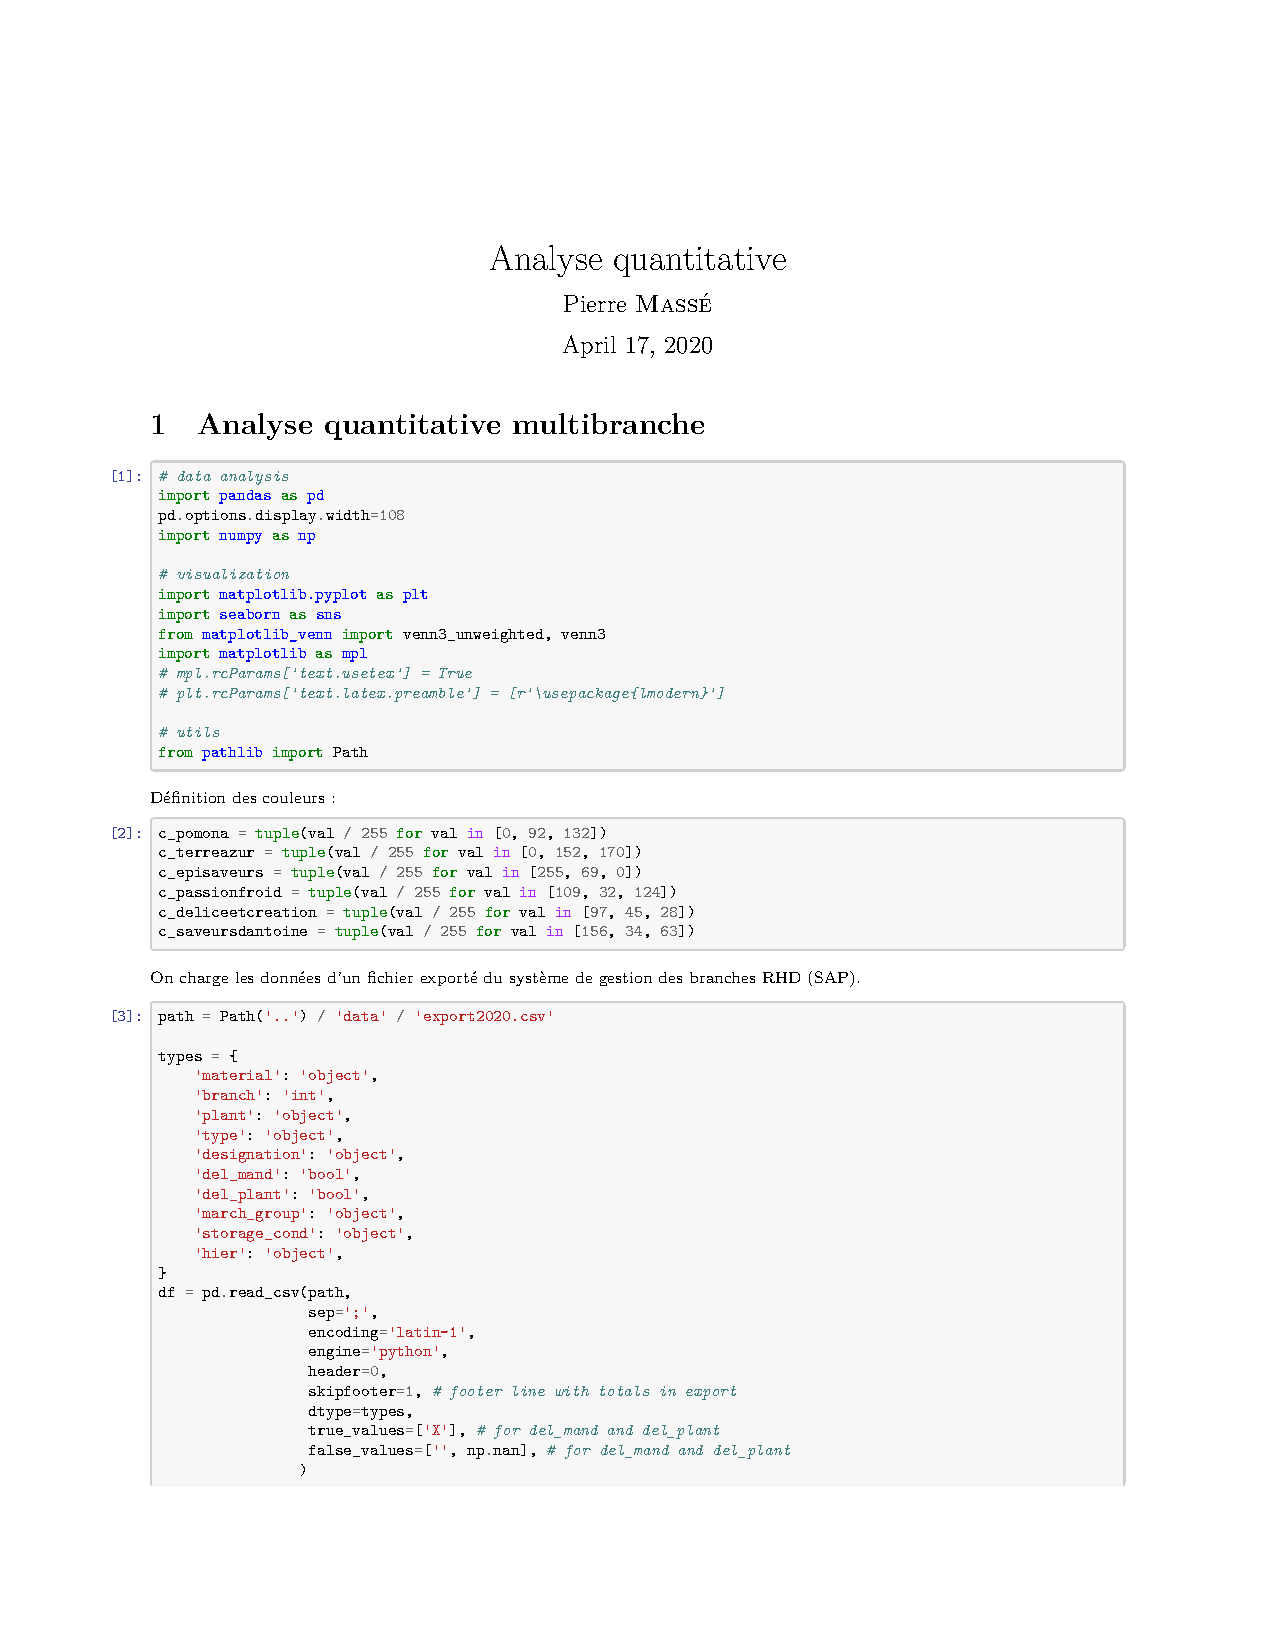
\includepdf[pages=-,
                    pagecommand={},
                    addtotoc={1, section, 1, Analyse quantitative, code:analyse_quantitative}]
                    {notebooks/Analyse quantitative.pdf}
        
        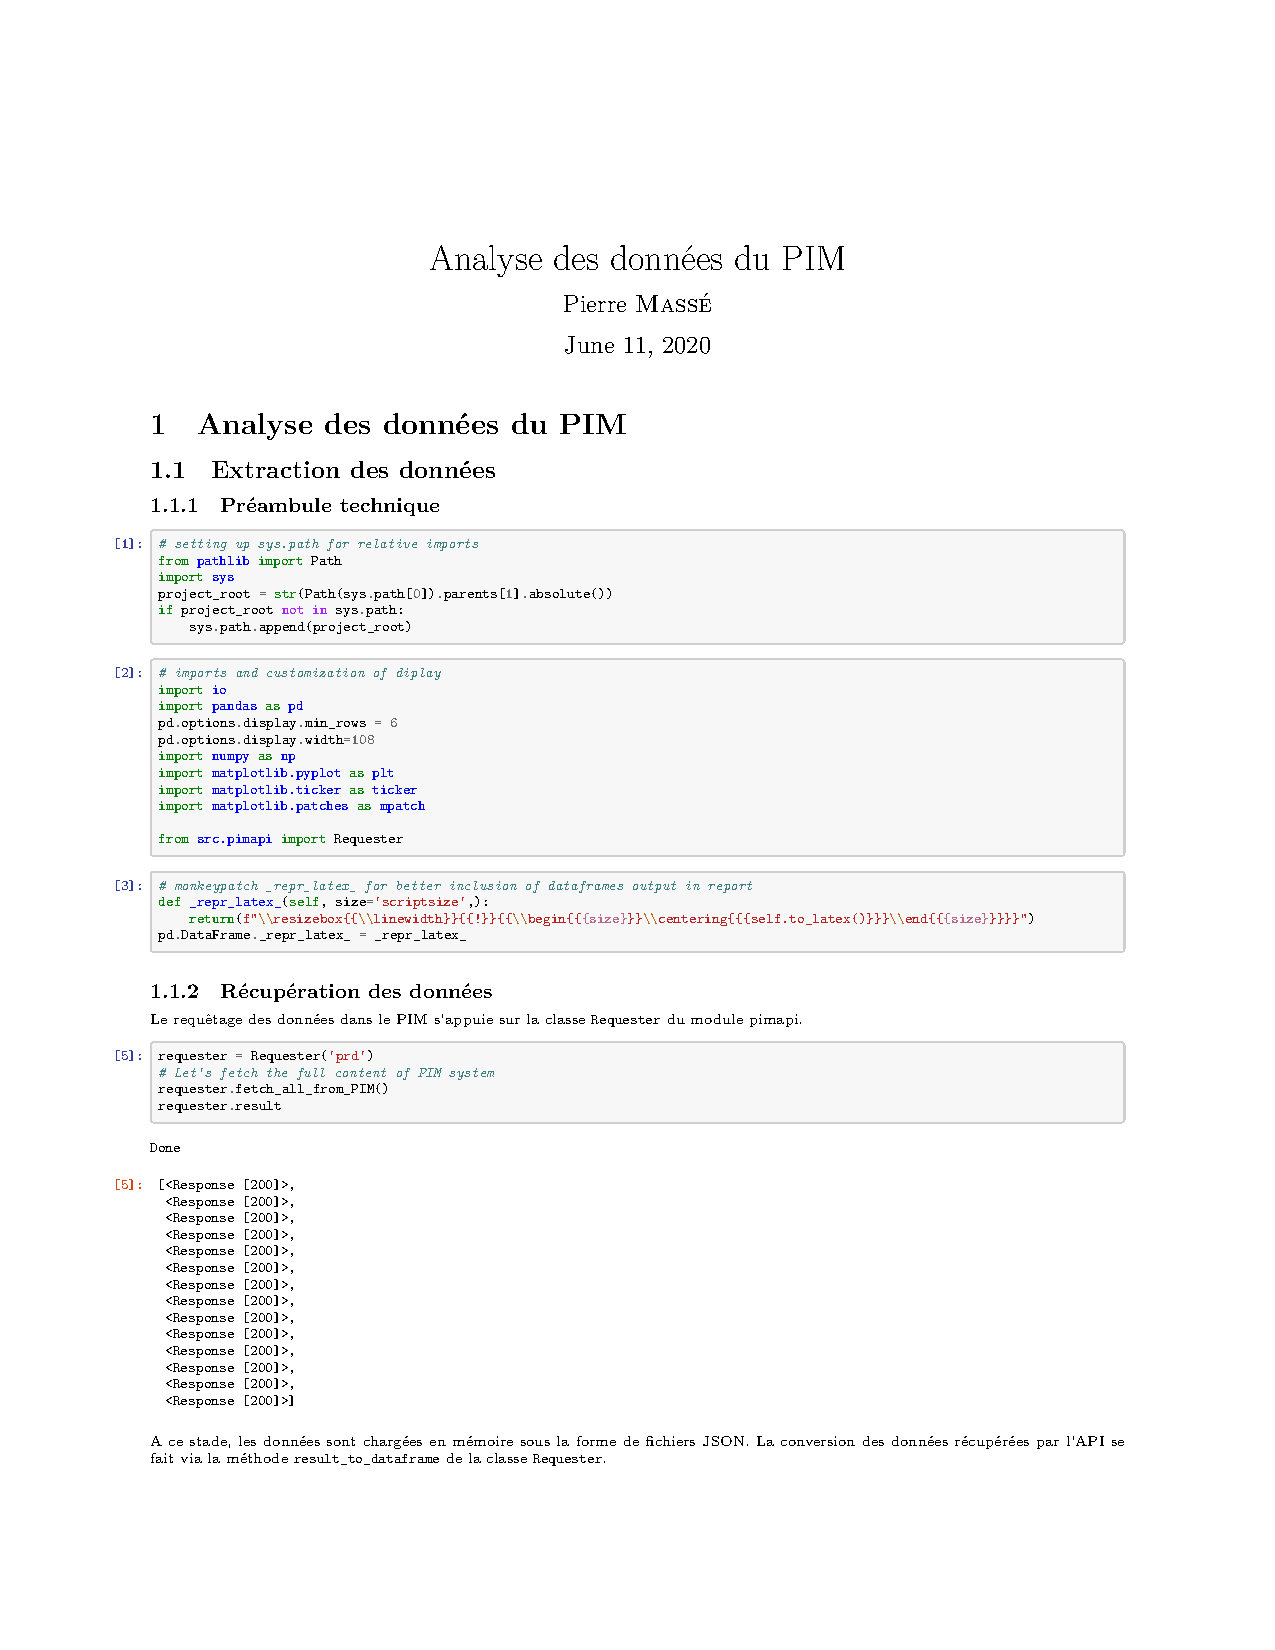
\includepdf[pages=-,
                    pagecommand={},
                    addtotoc={1,
                              section,
                              3,
                              Analyse des données du PIM,
                              code:analyse_donnees_PIM}]
                    {notebooks/Analyse donnees du PIM.pdf}

        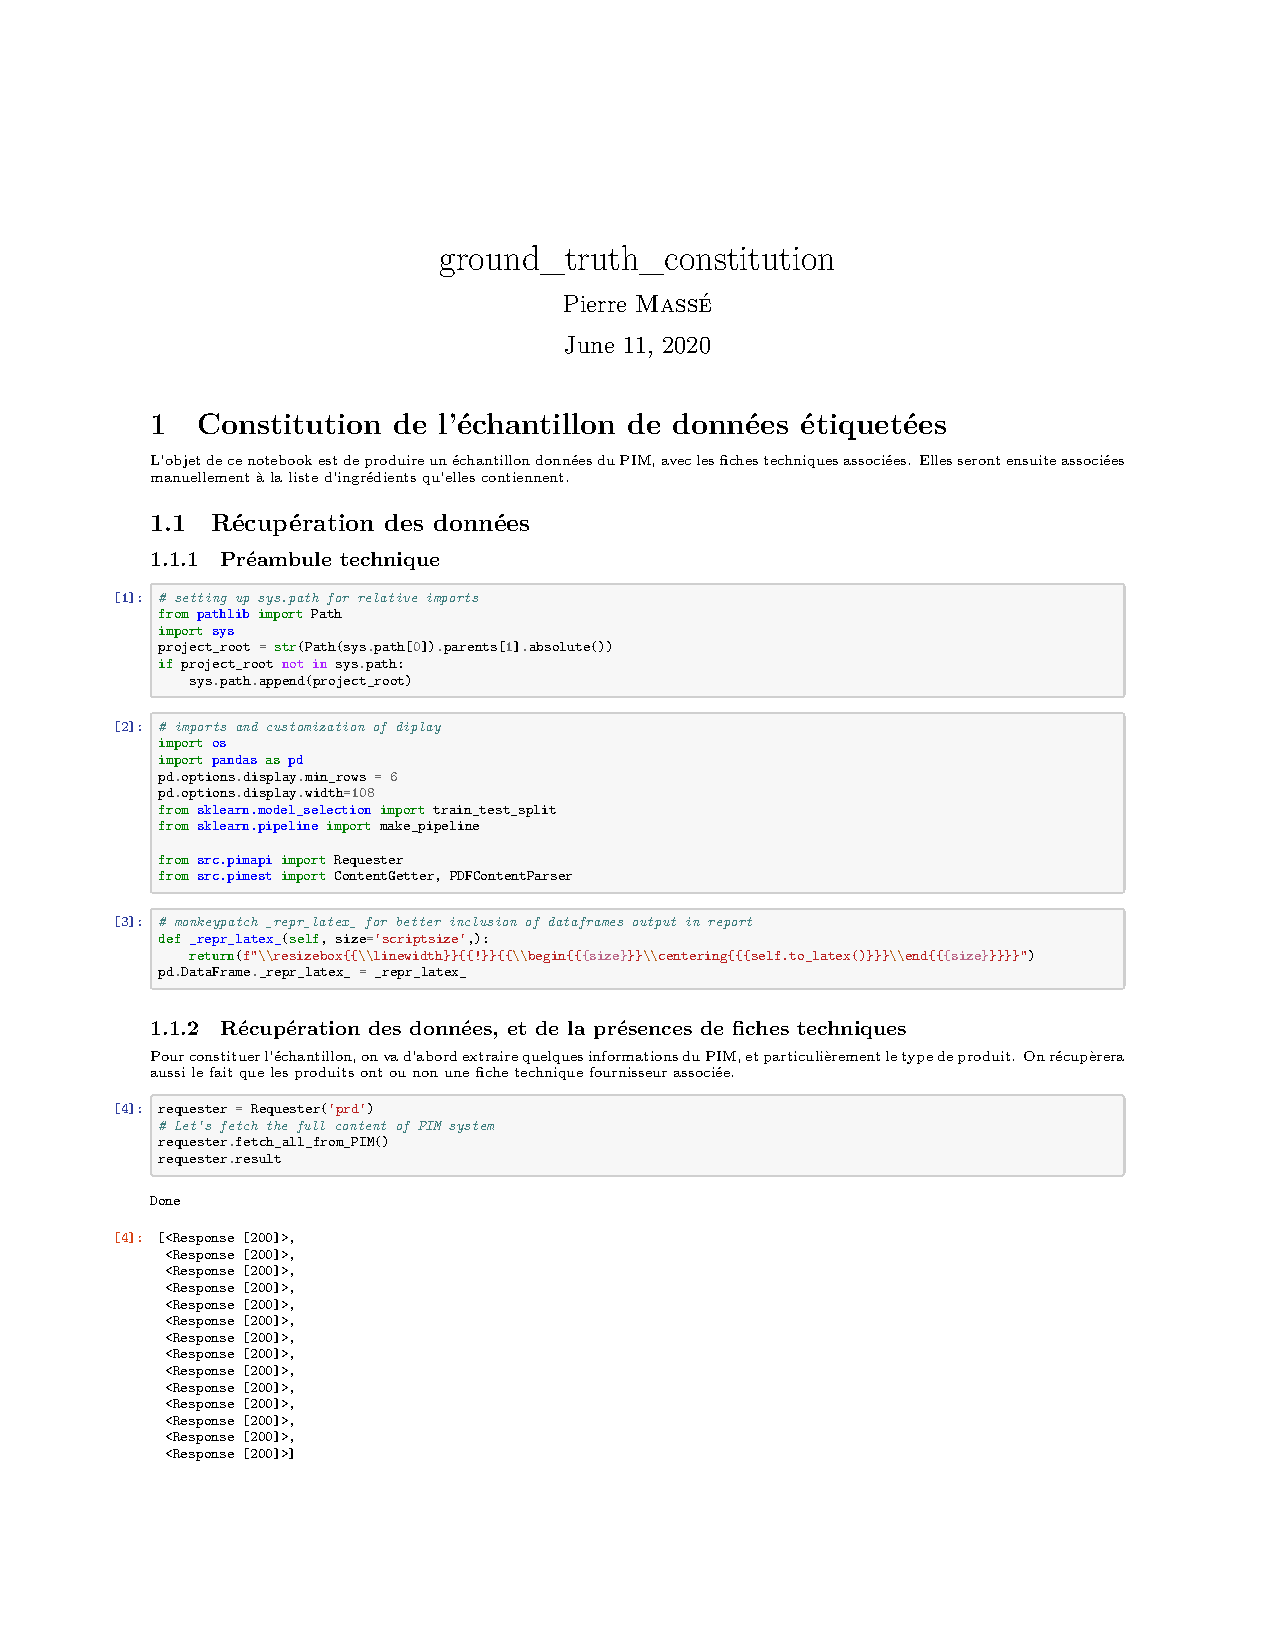
\includepdf[pages=-,
        pagecommand={},
        addtotoc={1, section, 1, Génération de l'échantillon de données manuellement étiquetées, code:ground_truth
                    }]
        {notebooks/ground_truth_constitution.pdf}

        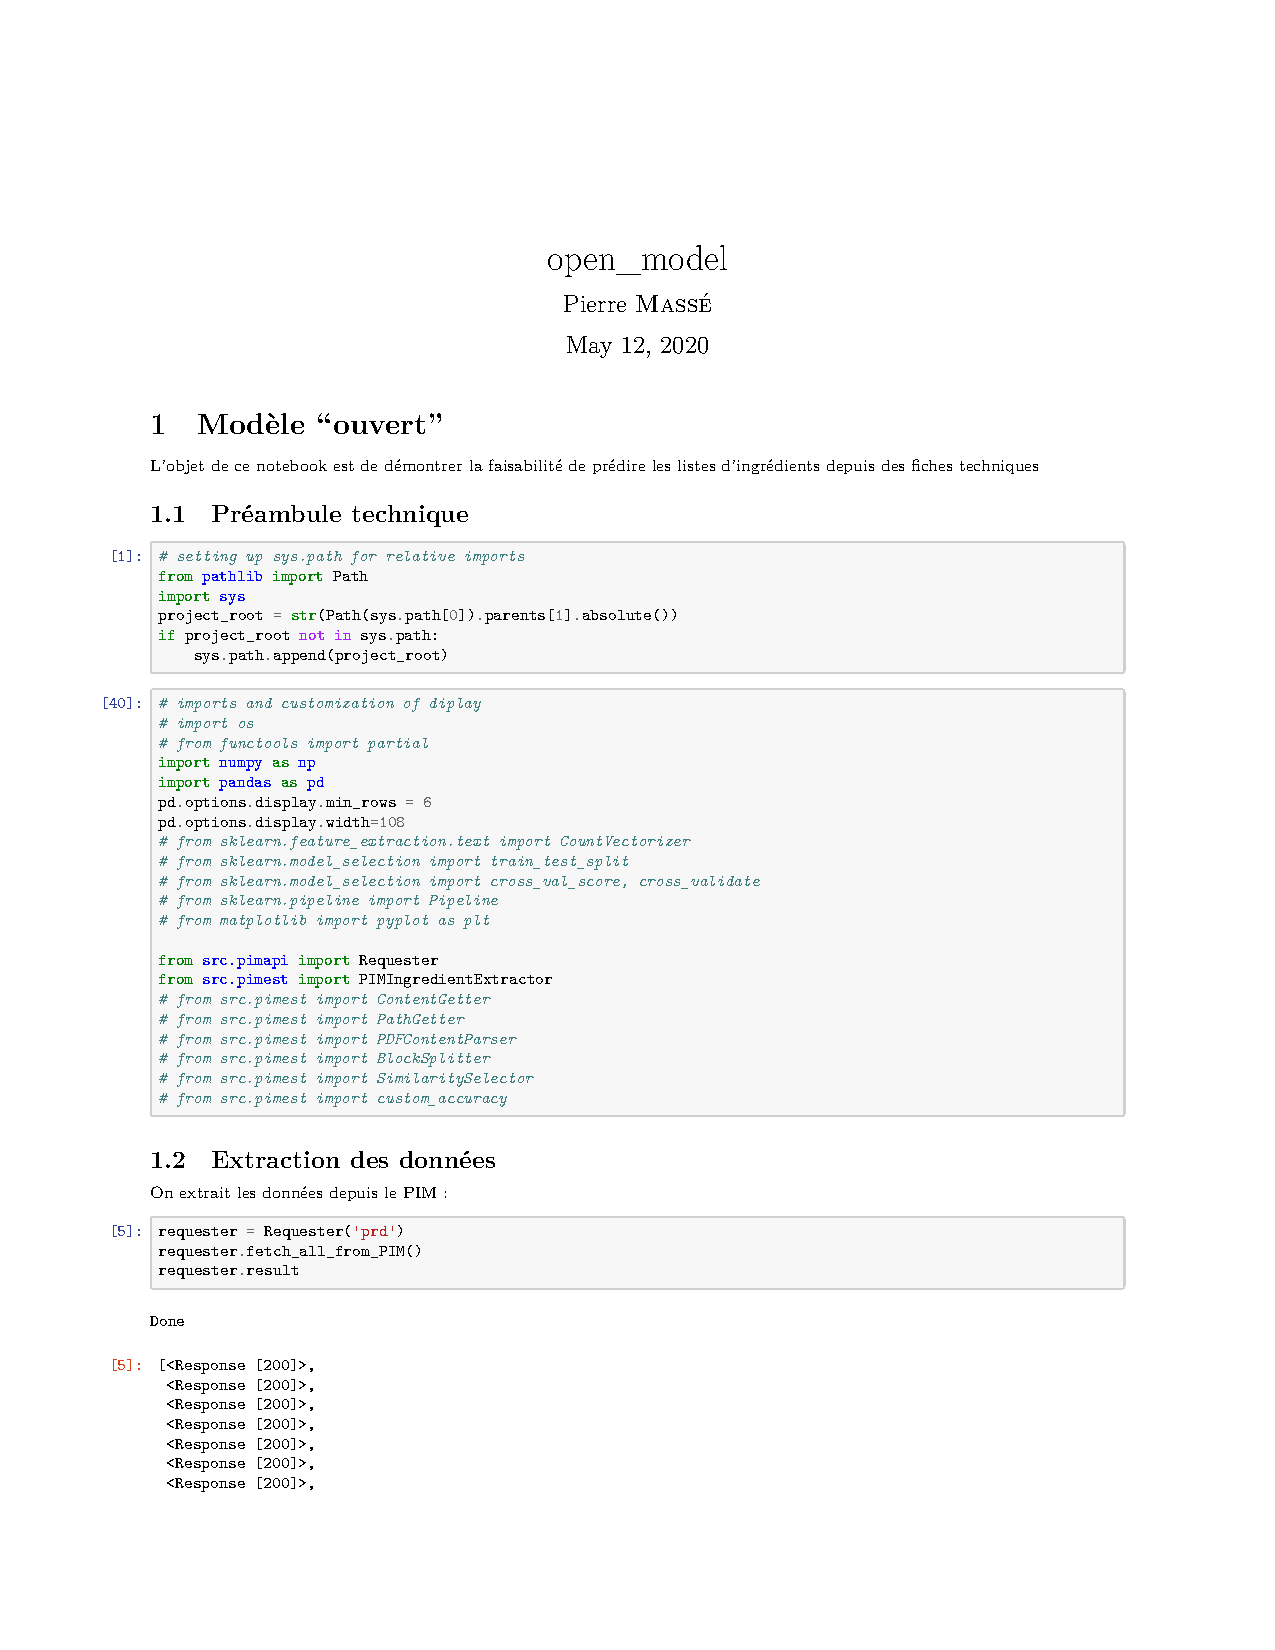
\includepdf[pages=-,
        pagecommand={},
        addtotoc={1, section, 1, Modèle \og ouvert \fg, code:open_model
                    }]
        {notebooks/open_model.pdf}
 
        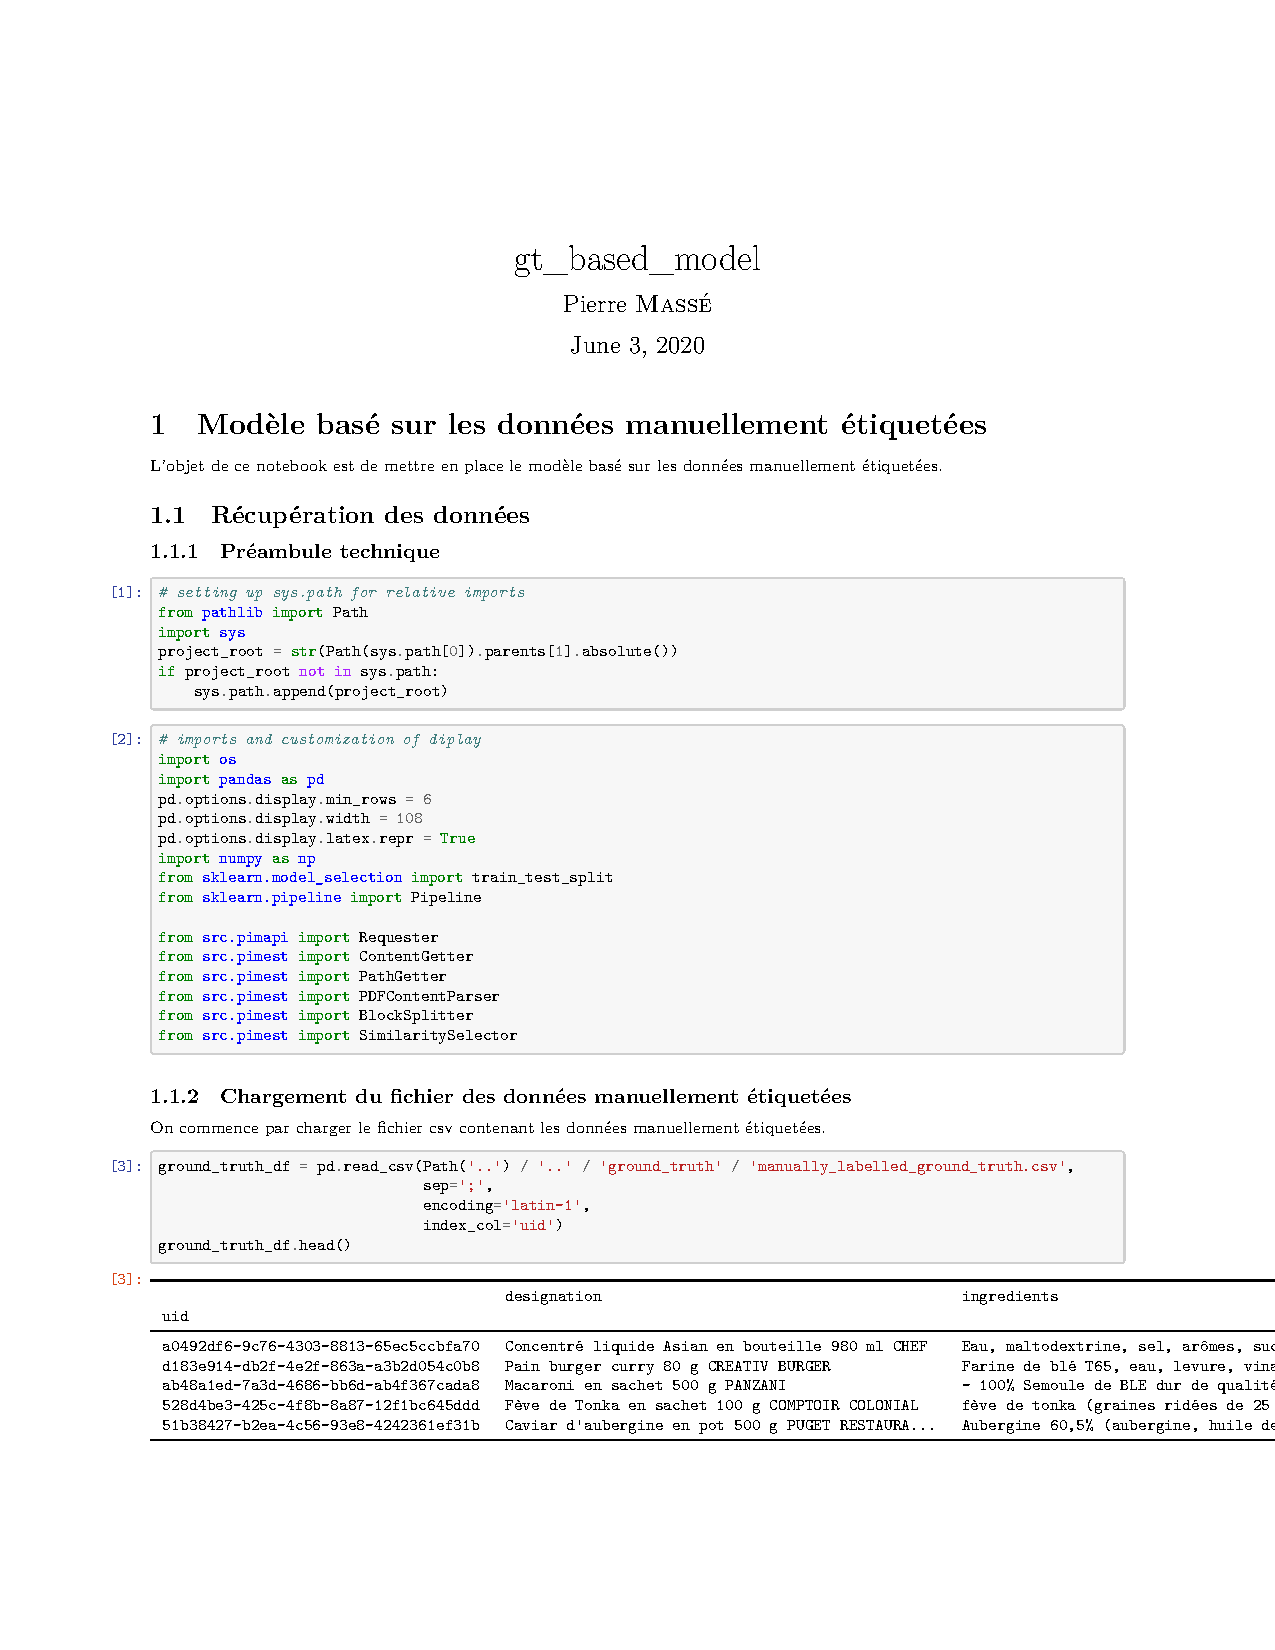
\includepdf[pages=-,
        pagecommand={},
        addtotoc={1, section, 1, Modèle basé sur les données manuellement étiquetées, code:gt_based_model
                    }]
        {notebooks/gt_based_model.pdf}

        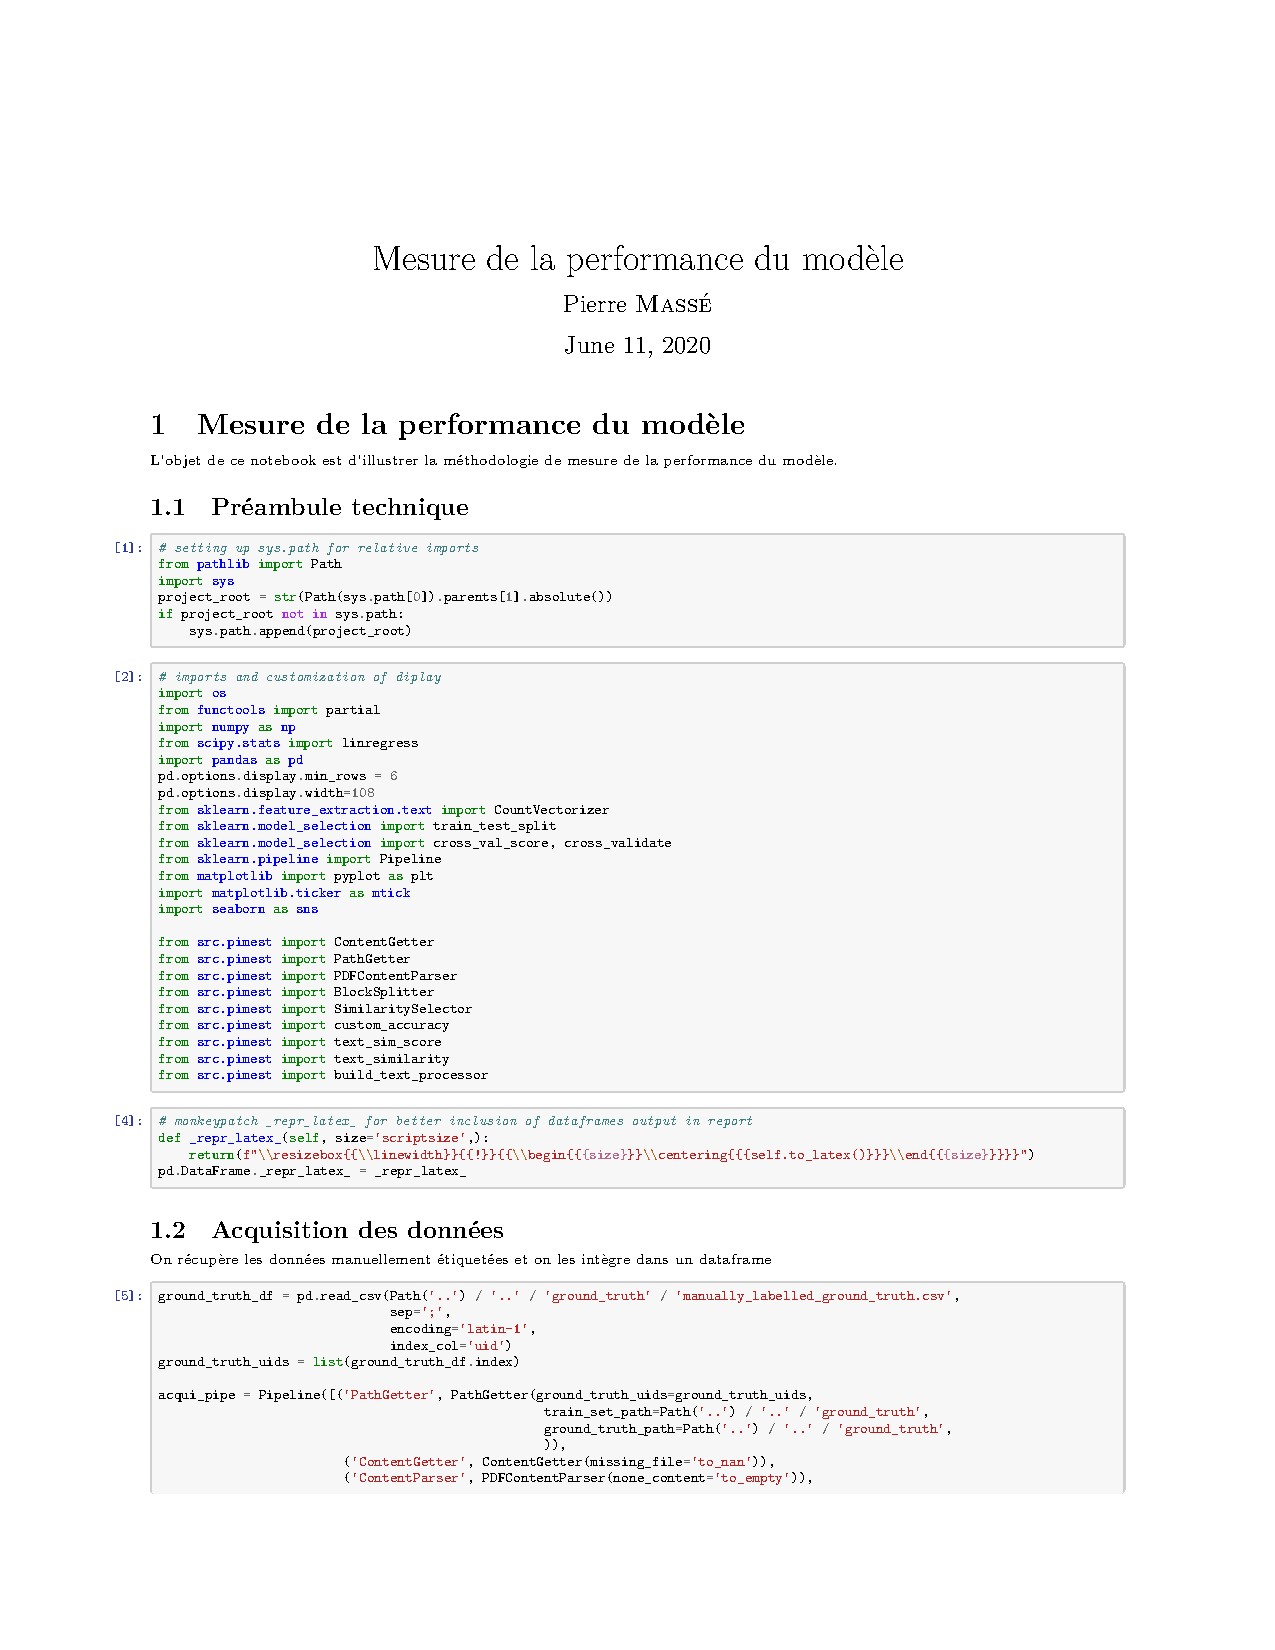
\includepdf[pages=-,
        pagecommand={},
        addtotoc={1, section, 1, Mesure de la performance, code:performance_measurement
                    }]
        {notebooks/Performance_measurement.pdf}        
    
    \chapter{Le code des différents modules}

    \section{Gestion du fichier de configuration - Module conf}
    \label{code:conf}
    Ce petit module a pour but de permettre de gérer les paramètres du progamme dans un fichier de configuration (afin de simplifier la maintenance).
    Il est utilisé dans l'ensemble des autres modules de ce projet.

    \begin{multicols}{2}
    \begin{spacing}{1.0}
        \inputminted[fontsize=\tiny]{python}{../src/conf.py}
    \end{spacing}
    \end{multicols}

    Un exemple de fichier de configuration (dont certains champs ont été anonymisés pour des raisons de confidentialité) est présenté ci-dessous.
    TODO !! Mettre le fichier ici.

    \section{Extraction des données du PIM - Module pimapi}
    \label{code:pimapi}
    \begin{multicols}{2}
    \begin{spacing}{1.0}
    \inputminted[fontsize=\tiny]{python}{../src/pimapi.py}
    \end{spacing}
    \end{multicols}

    \section{Conversion des pièces jointes en textes - Module pimpdf}
    \label{code:pimpdf}
    \begin{multicols}{2}
    \begin{spacing}{1.0}
    \inputminted[fontsize=\tiny]{python}{../src/pimpdf.py}
    \end{spacing}
    \end{multicols}
    
    \section{Transformateurs et estimateurs spécifiques - Module pimest}
    \label{code:pimest}

    Ce module définit divers estimateurs et transformateurs utilisés dans les modèles.
    Les fonctions de scoring, servant à la mesure de la performance, en font également partie.
    Les classes `IngredientExtractor` et `PIMIngredientExtractor` ont été construite au début des travaux sur le sujet, et sont donc plus \og brouillonnes \fg que le reste du code.
    
    \begin{multicols}{2}
    \begin{spacing}{1.0}
    \inputminted[fontsize=\tiny]{python}{../src/pimest.py}
    \end{spacing}
    \end{multicols}

\end{document}